%%%%%%%%%%%%%%%%%%%%%%%%%%%%%%%%%%%%%%%%%%%%%%%%%%%%%%%%%%%%%%%%%%%%%
%
% Complete documentation on the extended LaTeX markup used for Insight
% documentation is available in ``Documenting Insight'', that is part
% of the standard documentation for Insight.  It may be found online
% at:
%
%                    http://www.itk.org
%
%%%%%%%%%%%%%%%%%%%%%%%%%%%%%%%%%%%%%%%%%%%%%%%%%%%%%%%%%%%%%%%%%%%%%

\documentclass{InsightSoftwareGuide}

\usepackage[pdftex]{graphicx}

\usepackage{times,lscape,url}

\usepackage[latin1]{inputenc}

\usepackage{tikz}

\usepackage{color}

\usepackage{xspace}

\usepackage{longtable}

\definecolor{listcomment}{rgb}{0.0,0.5,0.0}
\definecolor{listkeyword}{rgb}{0.0,0.0,0.5}
\definecolor{listnumbers}{gray}{0.65}
\definecolor{listlightgray}{gray}{0.955}
\definecolor{listwhite}{gray}{1.0}

\usepackage{listings}
\newcommand{\lstsetcpp}
{
\lstset{frame = tb,
       framerule = 0.25pt,
       float,
       fontadjust,
       backgroundcolor={\color{listlightgray}},
       basicstyle = {\ttfamily\footnotesize},
       keywordstyle = {\ttfamily\color{listkeyword}\textbf},
       identifierstyle = {\ttfamily},
       commentstyle = {\ttfamily\color{listcomment}\textit},
       stringstyle = {\ttfamily},
       showstringspaces = false,
       showtabs = false,
       numbers = none,
       numbersep = 6pt,
       numberstyle={\ttfamily\color{listnumbers}},
       tabsize = 2,
       language=[ANSI]C++,
       floatplacement=!h
       }
}
\newcommand{\lstsetpython}
{
\lstset{language=Python
        }
}
\newcommand{\lstsetjava}
{
\lstset{language=Java
        }
}


\newif\ifitkFullVersion
\itkFullVersiontrue
%\itkFullVersionfalse

\newif\ifitkPrintedVersion
\itkPrintedVersiontrue
%\itkPrintedVersionfalse


%%%%%%%%%%%%%%%%%%%%%%%%%%%%%%%%%%%%%%%%%%%%%%%%%%%%%%%%%%%%%%%%%%
%
%  hyperref should be the last package to be loaded.
%
%%%%%%%%%%%%%%%%%%%%%%%%%%%%%%%%%%%%%%%%%%%%%%%%%%%%%%%%%%%%%%%%%%
\usepackage[pdftex,
pdftitle={The Orfeo ToolBox Cookbook, a guide for non-developers},
pdfauthor={CNES},
pdfsubject={Remote Sensing, Orfeo, Pleiades, Cosmo Skymed},
pdfkeywords={image processing, Remote sensing, Guide},
pdfpagemode={UseOutlines},
bookmarks,bookmarksopen,
pdfstartview={FitH},
backref,
colorlinks,linkcolor={red},citecolor={blue},urlcolor={blue},
]{hyperref}

\usepackage{amsmath,amssymb,amsfonts}
\usepackage{bbm}

\def\logoCNES{../Art/CNES_nom.pdf}



% Useful macros
\newcommand{\otb}{\textbf{Orfeo ToolBox}\xspace}
\newcommand{\app}{\textbf{OTB Applications}\xspace}
\newcommand{\mont}{\textbf{Monteverdi}\xspace}
\newcommand{\jpg}{\href{http://en.wikipedia.org/wiki/JPEG_2000}{Jpeg2000}\xspace}
\newcommand{\phr}{\href{http://smsc.cnes.fr/PLEIADES/index.htm}{Pleiades}\xspace}
\newcommand{\mmod}[1]{\emph{#1}\index{#1}\xspace}
\newcommand{\application}[1]{\emph{#1}\index{#1}\xspace}
\newcommand{\ossim}{\href{http://www.ossim.org/OSSIM/OSSIM_Home.html}{OSSIM}\xspace}
\newcommand{\sg}{\href{http://orfeo-toolbox.org/SoftwareGuide/}{OTB Software Guide}\xspace}
\newcommand{\dox}{\href{http://orfeo-toolbox.org/doxygen/}{Doxygen}\xspace}
\newcommand{\website}{\href{http://orfeo-toolbox.org}{Orfeo ToolBox website}\xspace}
\newcommand{\qgis}{\href{http://www.qgis.org/}{Quantum GIS}\xspace}
\newcommand{\gdal}{\href{http://www.gdal.org/}{GDAL}\xspace}
\newcommand{\osgeow}{\href{http://trac.osgeo.org/osgeo4w/}{OSGeo4W}\xspace}
\newcommand{\download}{\href{http://sourceforge.net/projects/orfeo-toolbox/}{OTB download
   page}\xspace}
\newcommand{\googleearth}{\textbf{Google Earth\copyright}\xspace}

\newtheorem{algo}{Algorithm}
\newtheorem{defin}{Definition}

\title{The Orfeo ToolBox Cookbook, a guide for non-developers\\ Updated
  for OTB-3.17}

\author{OTB Development Team}

\authoraddress{
  \url{http://www.orfeo-toolbox.org}\\
  e-mail: \email{otb@cnes.fr}
}

\date{\today}


% actually write the .idx file
\makeindex

\setcounter{tocdepth}{3}

%%%%%%%%%%%%%%%%%%%%%%%%%%%%%%%%%%%%%%%%%%%%%%%%%%%%%%%%%%%%%%%%%%%
%
%           Begin Document
%
%%%%%%%%%%%%%%%%%%%%%%%%%%%%%%%%%%%%%%%%%%%%%%%%%%%%%%%%%%%%%%%%%%%

\begin{document}

\ifitkPrintedVersion
\fi

\maketitle

\frontmatter

\hyperbaseurl{http://www.orfeo-toolbox.org}

\lstsetcpp

%%%%%%%%%%%%%%%%%%%%%%%%%%%%%%%%%%%%%%%%%%
%
%  Page with OTB logo
%
%%%%%%%%%%%%%%%%%%%%%%%%%%%%%%%%%%%%%%%%%%
\cleardoublepage

\begin{minipage}[t][10cm][b]{\textwidth}
\center
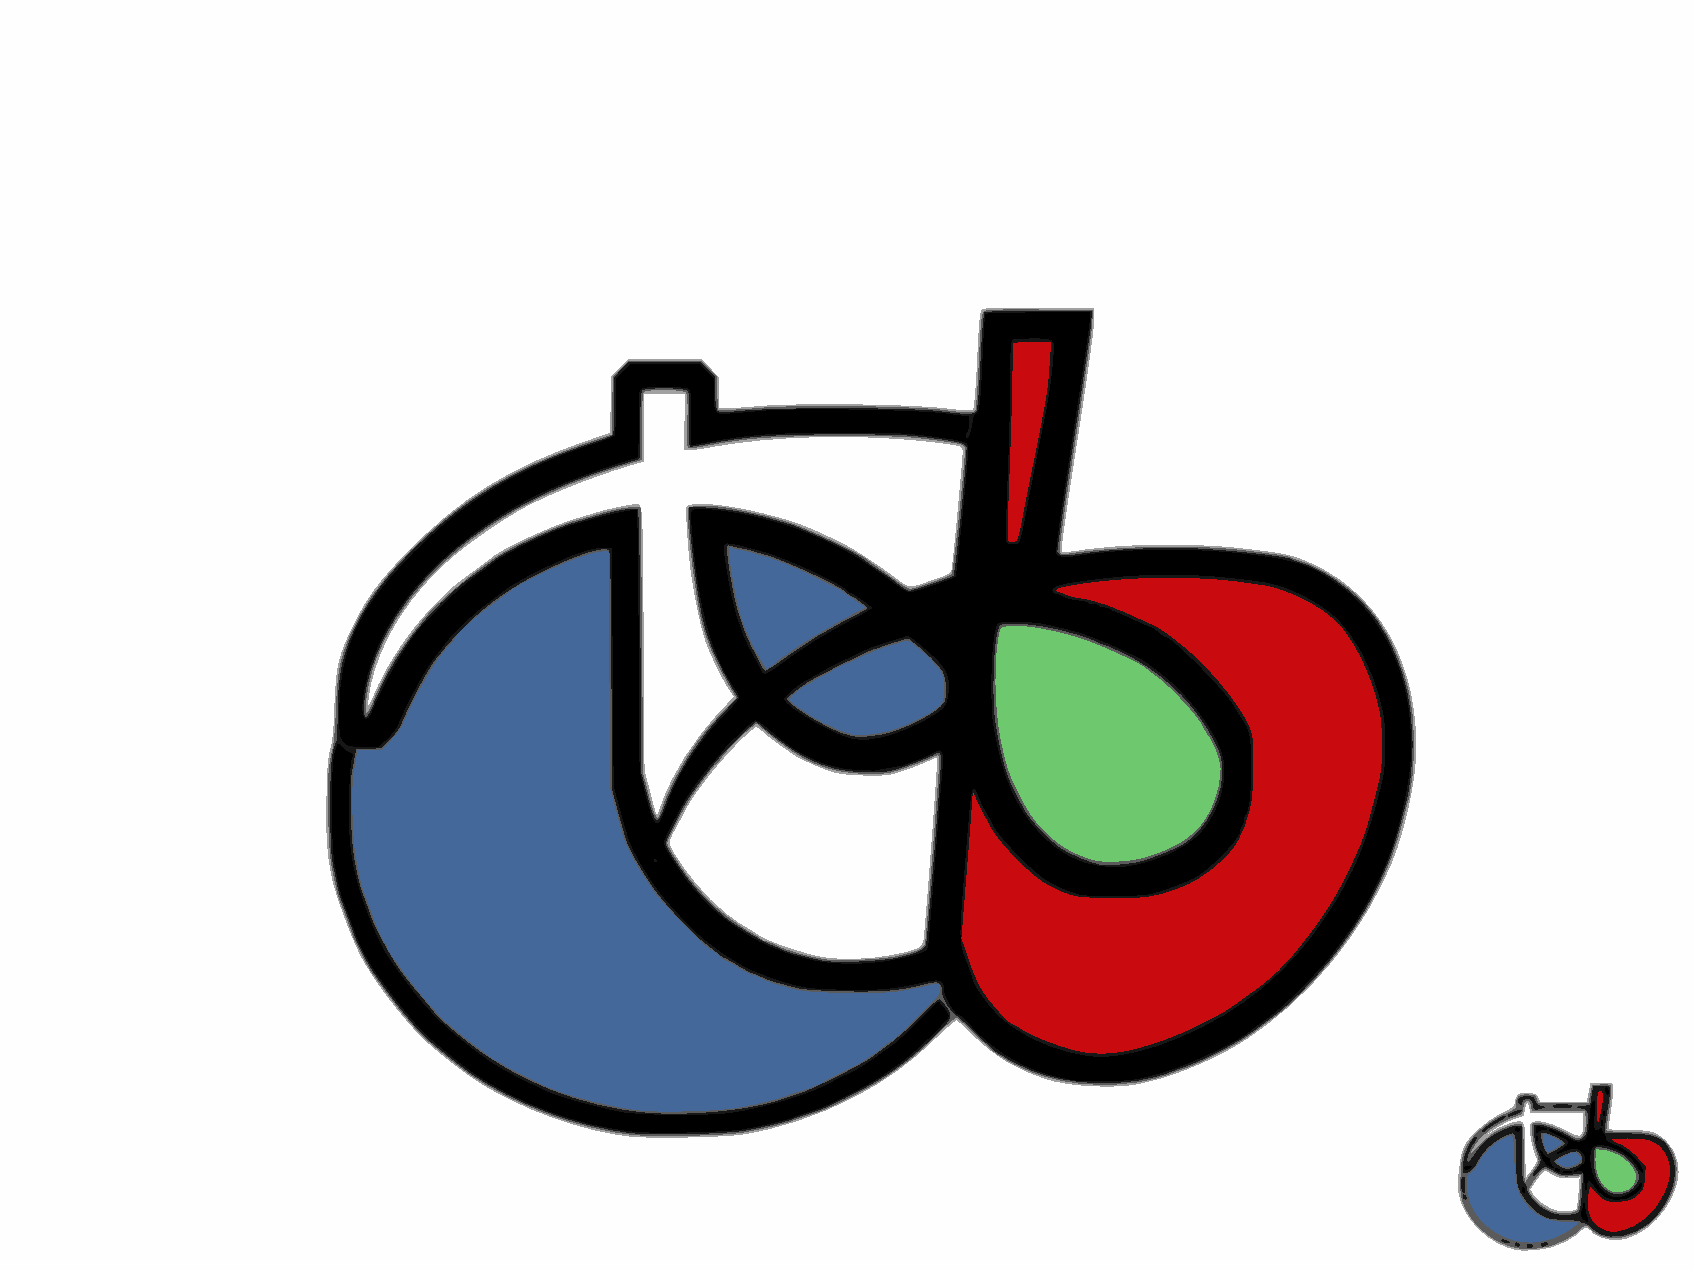
\includegraphics[width=0.5\textwidth]{../Art/logoVectoriel.pdf}
\large
\begin{center}
\emph{The ORFEO Toolbox is not a black box.}\\
\end{center}
\hspace{8cm} Ch.D.
\normalsize
\end{minipage}

%%%%%%%%%%%%%%%%%%%%%%%%%%%%%%%%%%%%%%%%%%%%%%
%
% remove headings from the following material
\pagestyle{plain}
%
%%%%%%%%%%%%%%%%%%%%%%%%%%%%%%%%%%%%%%%%%%%%%%

%%\ifitkPrintedVersion
%% % We want this material to fit on two pages
\small

\chapter*{About the Cover}

Creating the cover image demonstrating the capabilities of the toolkit was a
challenging task.\footnote{The source code for the cover is available from
InsightDocuments/SoftwareGuide/Cover/Source/.} Given that the origins of ITK
are with the Visible Human Project it seemed appropriate to create an image
utilizing the VHP data sets, and it was decided to use the more recently
acquired Visible Woman dataset.  Both the RGB cryosections and the CT scans
were combined in the same scene.

\begin{description}

\item [Removing the Gel.]
The body of the Visible Woman was immersed in a block of gel during the
freezing process. This gel appears as a blue material in the cryogenic data.
To remove the gel, the joint histogram of RGB values was computed. This
resulted in an 3D image of $256\times256\times256$ pixels. The histogram
image was visualized in VolView.\footnote{VolView is a commercial product
from Kitware. It supports ITK plug-ins and is available as a free viewer or
may be licensed with advanced functionality. See
http://www.kitware.com/products/volview.html for information.} The cluster
corresponding to the statistical distribution of blue values was identified
visually, and a separating plane was manually defined in RGB space. The
equation of this plane was subsequently used to discriminate pixels in the
gel from pixels in the anatomical structures. The gel pixels were zeroed out
and the RGB values on the body were preserved.

\item[The Skin.]
The skin was easy to segment once the gel was removed. A simple region
growing algorithm was used requiring seed points in the region previously
occupied by the gel and then set to zero values. An anti-aliasing filter was
applied in order to generate an image of pixel type float where the surface
was represented by the zero set. This data set was exported to VTK where a
contouring filter was used to extract the surface and introduce it in the VTK
visualization pipeline.

\item[The Brain.]
The visible part of the brain represents the surface of the gray matter.  The
brain was segmented using the vector version of the confidence connected
image filter.  This filter implements a region growing algorithm that starts
from a set of seed points and adds neighboring pixels subject to a condition
of homogeneity.

The set of sparse points obtained from the region growing algorithm was
passed through a mathematical morphology dilation in order to close holes and
then through a binary median filter. The binary median filter has the
outstanding characteristic of being very simple in implementation by applying
a sophisticated effect on the image. Qualitatively it is equivalent to a
curvature flow evolution of the iso-contours. In fact the binary median
filter as implemented in ITK is equivalent to the majority filter that
belongs to the family of voting filters classified as a subset of the
\emph{Larger than Life} cellular automata. Finally, the volume resulting from
the median filter was passed through the anti-aliasing image filter. As
before, VTK was used to extract the surface.

\item[The Neck Musculature.]
The neck musculature was not perfectly segmented. Indeed, the resulting
surface is a fusion of muscles, blood vessels and other anatomical
structures. The segmentation was performed by applying the
VectorConfidenceConnectedImageFilter to the cryogenic dataset. Approximately
60 seed points were manually selected and then passed to the filter as
input. The binary mask produced by the filter was dilated with a mathematical
morphology filter and smoothed with the BinaryMedianImageFilter. The
AntiAliasBinaryImageFilter was used at the end to reduce the pixelization
effects prior to the extraction of the iso-surface with vtkContourFilter.

\item[The Skull.]
The skull was segmented from the CT data set and registered to the cryogenic
data. The segmentation was performed by simple thresholding, which was good
enough for the cover image. As a result, most of the bone structures are
actually fused together. This includes the jaw bone and the cervical
vertebrae.

\item[The Eye.] 
The eye is charged with symbolism in this image. This is due in part because
the motivation for the toolkit is the analysis of the Visible Human data,
and in part because the name of the toolkit is \emph{Insight}.

The first step in processing the eye was to extract a sub-image of
$60\times60\times60$ pixels centered around the eyeball from the RGB
cryogenic data set. This small volume was then processed with the vector
gradient anisotropic diffusion filter in order to increase the homogeneity of
the pixels in the eyeball.

The smoothed volume was segmented using the
VectorConfidenceConnectedImageFilter using 10 seed points. The resulting
binary mask was dilated with a mathematical morphology filter with a
structuring element of radius one, then smoothed with a binary mean image
filter (equivalent to majority voting cellular automata). Finally the mask
was processed with the AntiAliasBinaryImageFilter in order to generate a
float image with the eyeball contour embedded as a zero set.

\item[Visualization.]
The visualization of the segmentation was done by passing all the binary
masks through the AntiAliasBinaryImageFilter, generating iso-contours with
VTK filters, and then setting up a VTK Tcl script. The skin surface was
clipped using the vtkClipPolyDataFilter using the implicit function
vtkCylinder. The vtkWindowToImageFilter proved to be quite useful for
generating the final high resolution rendering of the scene ($3000\times3000$
pixels).

\item[Cosmetic Postprocessing.]
We have to confess that we used Adobe Photoshop to post-process the image. In
particular, the background of the image was adjusted using Photoshop's color
selection. The overall composition of the image with the cover text and
graphics was also performed using Photoshop.

\end{description}

\normalsize

%%\fi

%\chapter*{Foreword}
\noindent


Beside the Pleiades (PHR) and Cosmo-Skymed (CSK) systems developments
forming ORFEO, the dual and bilateral system (France - Italy) for
Earth Observation, the ORFEO Accompaniment Program was set up, to
prepare, accompany and promote the use and the exploitation of the
images derived from these sensors.

The creation of a preparatory
program\footnote{http://smsc.cnes.fr/PLEIADES/A\_prog\_accomp.htm} is
needed because of:
\begin{itemize}
\item the new capabilities and performances of the ORFEO systems
  (optical and radar high resolution, access capability, data quality,
  possibility to acquire simultaneously in optic and radar),
\item the implied need of new methodological developments : new
  processing methods, or adaptation of existing methods,
\item the need to realise those new developments in very close
  cooperation with the final users for better integration of new
  products in their systems.

\end{itemize}

This program was initiated by CNES mid-2003 and will last until mid
2013.  It consists in two parts, between which it is necessary to keep
a strong interaction:
\begin{itemize}
\item A Thematic part,
\item A Methodological part.
\end{itemize}

The Thematic part covers a large range of applications (civil and
defence), and aims at specifying and validating value added products
and services required by end users. This part includes consideration
about products integration in the operational systems or processing
chains. It also includes a careful thought on intermediary structures
to be developed to help non-autonomous users. Lastly, this part aims
at raising future users awareness, through practical demonstrations
and validations.

The Methodological part objective is the definition and the
development of tools for the operational exploitation of the
submetric optic and radar images (tridimensional aspects, changes
detection, texture analysis, pattern matching, optic radar
complementarities). It is mainly based on R\&D studies and doctorate
and post-doctorate researches.

In this context, CNES\footnote{http://www.cnes.fr} decided to develop
the \emph{ORFEO ToolBox} (OTB), a set of algorithms encapsulated in a
software library. The goals of the OTB is to capitalise a methological
\textit{savoir faire} in order to adopt an incremental development
approach aiming to efficiently exploit the results obtained in the
frame of methodological R\&D studies.

All the developments are based on FLOSS (Free/Libre Open Source
Software) or existing CNES developments. OTB is distributed under the
C\'eCILL licence,
\url{http://www.cecill.info/licences/Licence_CeCILL_V2-en.html}.

OTB is implemented in C++ and is mainly based on
ITK\footnote{http://www.itk.org} (Insight Toolkit).


%% L'environnement de l'OTB est mis en place par l'outil CMake\footnote{http://www.cmake.org},
%% permettant ainsi de g\'{e}rer les proc\'{e}dures de compilation, g\'{e}n\'{e}ration et d'installation et ce quelque sois la plate forme cible.

%% Dans un souci d'homog\'{e}n\'{e}isation, l'OTB est con\c{c}ue et d\'{e}velopp\'{e}e suivant la philosophie et les principes \'{e}dict\'{e}s
%% par la biblioth\`{e}que ITK (programmation g\'{e}n\'{e}rique, m\'{e}canisme des \emph{Object Factories}, \emph{Smart pointers}, exceptions, \emph{Multi-Threading}, etc...).
%% Ces principes sont pr\'{e}sent\'{e}s dans le paragraphe \emph{3.2 Essential System Concepts} du guide ITK \url{http://www.itk.org/ItkSoftwareGuide.pdf}

%% Enfin, la m\'{e}thodologie de d\'{e}veloppement appliqu\'{e}e s'appuie sur une approche it\'{e}rative bas\'{e}e sur la programmation agile :
%% le sch\'{e}ma de d\'{e}veloppement suit le cycle \'{e}dict\'{e}e par la m\'{e}thodolgie de l'eXtreme Programming (XP)\footnote{http://www.xprogramming.com}.



%% Ce document constitue le guide d'utilisation et de d\'{e}veloppement de l'OTB. La version la plus r\'{e}cente de ce document est accessible \`{a}
%% \url{http://smsc.cnes.fr/PLEIADES/Fr/A_prog_accomp.htm/OTB/otbSoftwareGuide.pdf}.



\chapter*{Foreword}
\noindent
After almost 5 years of development, the \otb has become a
rich library used in many remote sensing context, from research work
to operational systems. The \app and more recently the
Monteverdi tool has helped to broaden the audience of the library,
giving access to its functionalities to non-developers.

Meanwhile, the \sg has grown to more
than 700 pages of documented code examples, which, combined with the
class documentation with the \dox, allows developer users to find
their way through the \otb so as to write code suiting their
needs.

Yet, the documentation available for non-developers users, using
Monteverdi and \app to perform everyday remote sensing tasks, has been
almost inexistent for all these years, and these users had to learn
the software by themselves or ask for help from more experienced
users. This cookbook aims at fulfilling the need for an appropriate
documentation of the applications built upon the \otb: \mont, and
\app, which are now integrated into the main \otb package and provide
several access mode (command-line, QT interface, QGis plugins, other
languages \ldots).

A general introduction to these tools is first presented, along
with installation instructions. Rather than describing all modules and
applications in an exhaustive way, we then decided to focus on very
common remote sensing tasks, detailing how they can be achieved with
either \mont or an application.

For more information on the \otb, please feel free to visit the \website.

%%%%%%%%%%%%%%%%%%%%%%%%%%%%%%%%%%%%%%%%%%%%%%%%%%%%%%%%%
%
% Insert Table of Contents; List of Figures and Tables
%
%%%%%%%%%%%%%%%%%%%%%%%%%%%%%%%%%%%%%%%%%%%%%%%%%%%%%%%%%


%%%%%%%%%%%%%%%%%%%%%%%%%%%%%%%%%%%%%%%%%%%%%%
%
% enable headings from the following material
\pagestyle{normal}
%
%%%%%%%%%%%%%%%%%%%%%%%%%%%%%%%%%%%%%%%%%%%%%%
\small
\tableofcontents
\listoffigures
\listoftables
\normalsize

%%%%%%%%%%%%%%%%%%%%%%%%%%%%%%%%%%%%%%%%%
%
% Begin technical content
%
%%%%%%%%%%%%%%%%%%%%%%%%%%%%%%%%%%%%%%%%%

\mainmatter

\chapter{A brief tour of OTB-Applications}\label{chap:otb-applications}

\section{Introduction}\label{sec:appintro}

OTB-Applications is perhaps the older package of the \otb
suite after the OTB package itself. Since the \otb is a
library providing remote sensing functionalities, the only
applications that were distributed at the beginning were the examples
from the Software Guide and the tests. These applications are very
useful for the developer because their code is very short and only
demonstrates one functionality at a time, but in many cases a real
application would require combining together two or more functions
from the \otb, and providing a higher level interface to
handle parameters, input and output data and communication with the
user nicely.

The \app package was originally designed to provide applications
performing simple remote sensing tasks, more complex than simple
examples from the Software Guide, and with a more user-friendly
interface (either graphical or command-line), to demonstrate the use
of the \otb functions. The most popular applications are maybe the
\application{otbImageViewerManager}, which allows to open a collection
of images and navigate in them, and the
\application{otbSupervisedClassificationApplication}, which allows to
delineate training regions of interest on the image and classify the
image with a SVM classifier trained with these regions. During the
first 3 years of the \otb development, many more applications have
been added to this package, to perform various tasks. Most of them
come with a graphical user interface, apart from some small utilities
that are command-line.  For a complete list of these applications,
please refer to section~\ref{sec:appstruct}.

The development and release of the \mont software (see
chapter~\ref{chap:Monteverdi} at the end of year 2009 changed a lot of
things for the \app package: most of non-developer users were looking
for quite a long time for an applications providing \otb
functionalities under a unified graphical interface. Many applications
from the \app package were integrated to \mont as modules, and the
\app package lost a lot of its usefulness. No more applications were
added to the package and it was barely maintained, as new graphical
tools were directly embedded within \mont.

Then, some people started to regain interest in the \app package. \mont
is a great tool to perform numerous remote sensing and image
processing task in a minute, but it is not well adapted to heavier
(and longer) processing, scripting and batch processing. Therefore, in
2010 the \app package has been revamped: old applications have been
moved to a legacy folder for backward compatibility, and the
development team started to populate the package with compact
command-line tools to perform various heavy processing tasks. The
package is now rich of more than 40 tools, though not very well known
from the users for now. Although for now only the commmand-line
interface is fully functional, a work in progress aims at wrapping these
command-line tools to also offer QT graphical interfaces and integration
with the \qgis software as well as with other environment such as python,
IDL or Matlab (and with \mont).

\section{Installation}\label{sec:appinstall}

Detailed instruction on how to install the whole \otb suite either
from binary packages or from source are available in the \sg. Here, we
will focus only on the installation of the \app package from binary
package.

\subsection{Windows 2000/XP/Vista/Seven}
\label{ssec:app_windows_binaries}

For Windows 2000/XP/Vista/Seven users, an installation program exists
for OTB-Applications. This installers depends on dependencies that can
be installed through \osgeow. The packages that need to be installed
are \emph{gdal, curl, libtiff, libgeotiff, libjpeg, zlib and libpng}.

Remember that the corresponding dlls are to be accessible in the
system path. To ensure so, add the \osgeow bin directory to your
system path.

 Once the dependencies have been properly installed, please go the the
 \download, to get the installer. Double-click on the installer and
 let it guide you through the installation process.

\subsection{MacOS X}
\label{ssec:mac_binaries}

For now, no binary package is available for \app on MacOS X. You can
build the \app from sources by following instruction in the \sg.

\subsection{Linux}

\subsubsection{Ubuntu 10.04, 10.10 and 11.04}
\label{ssec:ubuntu_binaries}
For Unbuntu 10.04 (Lucid Lynx), 10.10 (Maverick Meerkat) and 11.04
(Natty Narwhal), the whole \otb suite is available through APT repositories.

If you are using apt command-line tools, use these command-lines to
add the otb repository to apt sources:
\begin{verbatim}
sudo aptitude install add-apt-repository 
sudo add-apt-repository ppa:otb/orfeotoolbox-stable
\end{verbatim}
Now run:
\begin{verbatim}
sudo aptitude update
sudo aptitude install otbapp
\end{verbatim}

If you are using \emph{Synaptic}, you can add the repositories, update
and install the packages through the graphical interface.

If you want to use OTB with bleeding edge versions of gdal and qgis,
there is an alternate UbuntuGIS repository.  You can add it by using
these command-lines:
\begin{verbatim}
sudo aptitude install add-apt-repository 
sudo apt-add-repository ppa:ubuntugis/ubuntugis-unstable
sudo add-apt-repository ppa:otb/orfeotoolbox-stable-ubuntugis
\end{verbatim}
Now run:
\begin{verbatim}
sudo aptitude update
sudo aptitude install otbapp
\end{verbatim}

Be careful not to add the two repositories, since they may cause
incompatibilities.

For further informations about ubuntu packages go to
href{https://launchpad.net/~otb/+archive/orfeotoolbox-stable}{orfeotoolbox-stable
  launchpad page} and click on \textbf{Read about installing}.

\textbf{apt-add-repository} will try to retrieve the GPG keys of the
repositories to certify the origin of the packages. If you are behind
a http proxy, this step won't work and apt-add-repository will stall
and eventually quit. You can temporarily ignore this error and proceed
with the update step. Following this, aptitude update will issue a
warning about a signature problem. This warning won't prevent you from
installing the packages.

\subsubsection{OpenSuse 11.2 and higher}
\label{ssec:opensuse_binaries}

For OpenSuse 11.2 and higher, the whole \otb suite is available
through \emph{zypper}.

First, you need to add the appropriate repositories with these
command-lines (please replace $11.4$ by your OpenSuse version):
\begin{verbatim}
sudo zypper ar 
http://download.opensuse.org/repositories/games/openSUSE_11.4/ Games
sudo zypper ar 
http://download.opensuse.org/repositories/Application:/Geo/openSUSE_11.4/ GEO
sudo zypper ar 
http://download.opensuse.org/repositories/home:/tzotsos/openSUSE_11.4/ tzotsos
\end{verbatim}

Now run:
\begin{verbatim}
sudo zypper refresh
sudo zypper install Orfeo-Applications
\end{verbatim}

Alternatively you can use the One-Click Installer from the
\href{http://software.opensuse.org/search?q=Orfeo&baseproject=openSUSE\%3A11.4&lang=en&include_home=true&exclude_debug=true}{openSUSE
  Download page} or add the above repositories and install through
Yast Package Management.

In case you wish to test the latest version of the packages, you can run:
\begin{verbatim}
sudo zypper refresh
sudo zypper install Orfeo-Applications-beta
\end{verbatim}

\section{Structure of the package}\label{sec:appstruct}


%\chapter{Using OTB applications}\label{chap:WrappedApplications}

\section{Introduction}\label{sec:wrappedAppliIntro}
The \app package (see \ref{chap:otb-applications}) has brought a nice set of 
applications, along with several tools to launch them (command line, Qt,...).
As for the future of these applications, it has been decided to integrate 
them inside the \otb library. This migration has been an opportunity to 
enhance all the framework around the applications: not only new features have
 been added, but the interface with the developer has also been simplified. 
The new framework has inherited the wrappers from \app, and new ones have been
added. The development philosophy behind these applications is to provide users 
with modular functional blocs for remote sensing, ready to be integrated in any
environment. 

Because the applications are now a part of the library, their installation doesn't
require much effort: when building the \otb library, you can activate the applications 
with the CMake boolean option \code{BUILD\_APPLICATIONS}.

\section{List of applications}\label{sec:wrappedAppliList}
The documentation of the available applications is accessible 
\href{http://orfeo-toolbox.org/Applications}{here}. Most of the old applications have
been migrated. They are sorted by categories.

\section{Available wrappers}\label{sec:wrappedAppliWrappers}

\subsection{Command line}\label{sec:wrappedAppliCmdLine}
By default, the applications can be called with the command line launcher. This launcher
is built in your \code{OTB\_DIR/bin} directory. It needs at least two arguments: the 
application name and the path to the \code{OTB\_DIR/bin} directory. Any additional argument
will be given to the application itself. You can ask the application to print its help
message:
\begin{verbatim}
otbApplicationLauncherCommandLine Rescale OTB_DIR/bin -help
\end{verbatim}
The help message (but also the \href{http://orfeo-toolbox.org/Applications}{documentation})
will give you the list of available parameters. Each parameter must be set by giving the 
corresponding key followed by its value:
\begin{verbatim}
otbApplicationLauncherCommandLine Rescale OTB_DIR/bin -in QB_Toulouse_Ortho_PAN.tif -out QB_Toulouse_rescaled.tif -outmin 0 -outmax 255
\end{verbatim}

If the application has sub-parameters (i.e. parameters contained in other parameters), 
their keys must be prefixed by their full tree path. For instance, the application 
\code{OrthoRectification} has a paramater for bicubic interpolation radius whose key is \code{radius}.
This parameter should be called with the path \code{-interpolator.bco.radius}.

Note that some types of parameters allow you to give several values after the key (they must
be separated with whitespaces).

For example an \emph{InputImageList} key, which can be followed by one or several filenames :

\begin{verbatim}
otbApplicationLauncherCommandLine ConcatenateImages OTB_DIR/bin -il GomaAvant.png GomaApres.png -out otbConcatenateImages.tif
\end{verbatim}


\subsection{Other wrappers}\label{sec:wrappedAppliOtherWrap}
If you want to use the other available wrappers, you have to activate the corresponding CMake 
options when building the library:
\begin{itemize}
  \item Enable \code{WRAP\_QT} to build a Qt application launcher. It opens a GUI which 
  allows you to set the parameters and execute the application. This launcher only needs 
  the same two arguments as the command line:
  \begin{verbatim}
  otbApplicationLauncherQt Rescale OTB\_DIR/bin
  \end{verbatim}
  It displays a window with several tabs. \textbf{[Parameters]} is where you set the parameters and execute the application.
  \textbf{[Logs]} is where you see the informations given by the application during its execution. \textbf{[Progress]} is 
  where you see a progress bar of the execution (not available for all applications). \textbf{[Documentation]} is where you
  find a summary of the application documentation.
   
  \item \code{WRAP\_PYTHON} : \textbf{TODO}
  \item \code{WRAP\_PYQT} : \textbf{TODO}
  \item \code{WRAP\_JAVA} : \textbf{TODO}
\end{itemize}



\chapter{A brief tour of \mont}\label{chap:Monteverdi} 

\section{Introduction}\label{sec:montintro}
The \app package makes available a set of simple software
tools, which were designed to demonstrate what can be done with
\otb. Many users started using these applications for real processing
tasks, so we tried to make them more generic, more robust and easy to
use. \otb users have been asking for an integrated application for a
while, since using several applications for a complete processing
(ortho-rectification, segmentation, classification, etc.) can be a
burden. The OTB team received a request from CNES' Strategy
and Programs Office in order to provide an integrated application for
capacity building activities (teaching, simple image manipulation,
etc.). The specifications included ease of integration of new
processing modules.  


\section{Installation}\label{sec:montinstall}

The application is called \mont, since this is the name of the Orfeo
composer. The application allows you to build interactivelly remote
sensing processes based on the \otb. This is also in
remembering of the great (and once open source) Khoros/Cantata
software.
  
Installation of \mont is very simple. Standard installer packages are available on the main platforms thanks to OTB-Developpers and external users. 
These packages are available few days after the release. Get the latest information on binary packages on the \website in the section download.

We will discribe in the following sections the way to install \mont on:
\begin{itemize}
\item Windows platform (XP/Seven)
\item Ubuntu 14.X and higher
\item MacOSX 10.10
\end{itemize}

If you want to build from source or if we don't provide packages for your system, some informations are available into the \sg, in the section \textbf(Building from Source).
Note that the git repository of \mont is located here : https://git.orfeo-toolbox.org/monteverdi2.git.
In order to get the source of \mont, you will ahve te be placed on the right branch : git checkout 3.0.0-rc1


\subsection{Windows XP/Seven/8.1}
For Windows XP/Seven/8.1 users, there is a classical standalone installation program for \mont, available from the \download after each release. 

It is also possible to get \mont package through \osgeow for Windows XP/Seven users. 
Package for \mont is available directly in the OSGeo4W installer when you select the \textbf{otb-monteverdi} package. 
Follow the instructions in the OSGeo4W installer and select the \textbf{otb-monteverdi}. 
The installer will proceed with the installation of the package and all its dependencies. 
\mont will be directly installed in the OSGeo4W repository and a shortcut will be added to your desktop and in the start menu (in the OSGeo4W folder). 
You can now use directly \mont from your desktop, from the start menu and from an OSGeo4W shell with command \texttt{monteverdi}. 
Currently, you should use the 32bit OSGeo4W installer but we will soon distribute \mont package for 64 bit installer. 

\subsection{MacOS X}
A standard DMG package is available for \mont for MacOS X 10.10. Please go the \download.
Click on the file to launch \mont. 

\subsection{Ubuntu 14.x and higher}
For Ubuntu 14.x and higher, \mont package may be available as Debian package through APT repositories.

You can add it by using these command-lines:
\begin{verbatim}
sudo aptitude install add-apt-repository
sudo apt-add-repository ppa:ubuntugis/ubuntugis-unstable
\end{verbatim}

Now run:
\begin{verbatim}
sudo aptitude install monteverdi
\end{verbatim}

If you are using \emph{Synaptic}, you can add the repository, update and install the package through the
graphical interface.

\textbf{apt-add-repository} will try to retrieve the GPG keys of the
repositories to certify the origin of the packages. If you are behind a http
proxy, this step won't work and apt-add-repository will stall and eventually
quit. You can temporarily ignore this error and proceed with the update
step. Following this, aptitude update will issue a warning about a signature
problem. This warning won't prevent you from installing the packages.


\section{GUI : what does it look like ?}\label{sec:mongui}


\begin{figure}[!h] 
  \center
  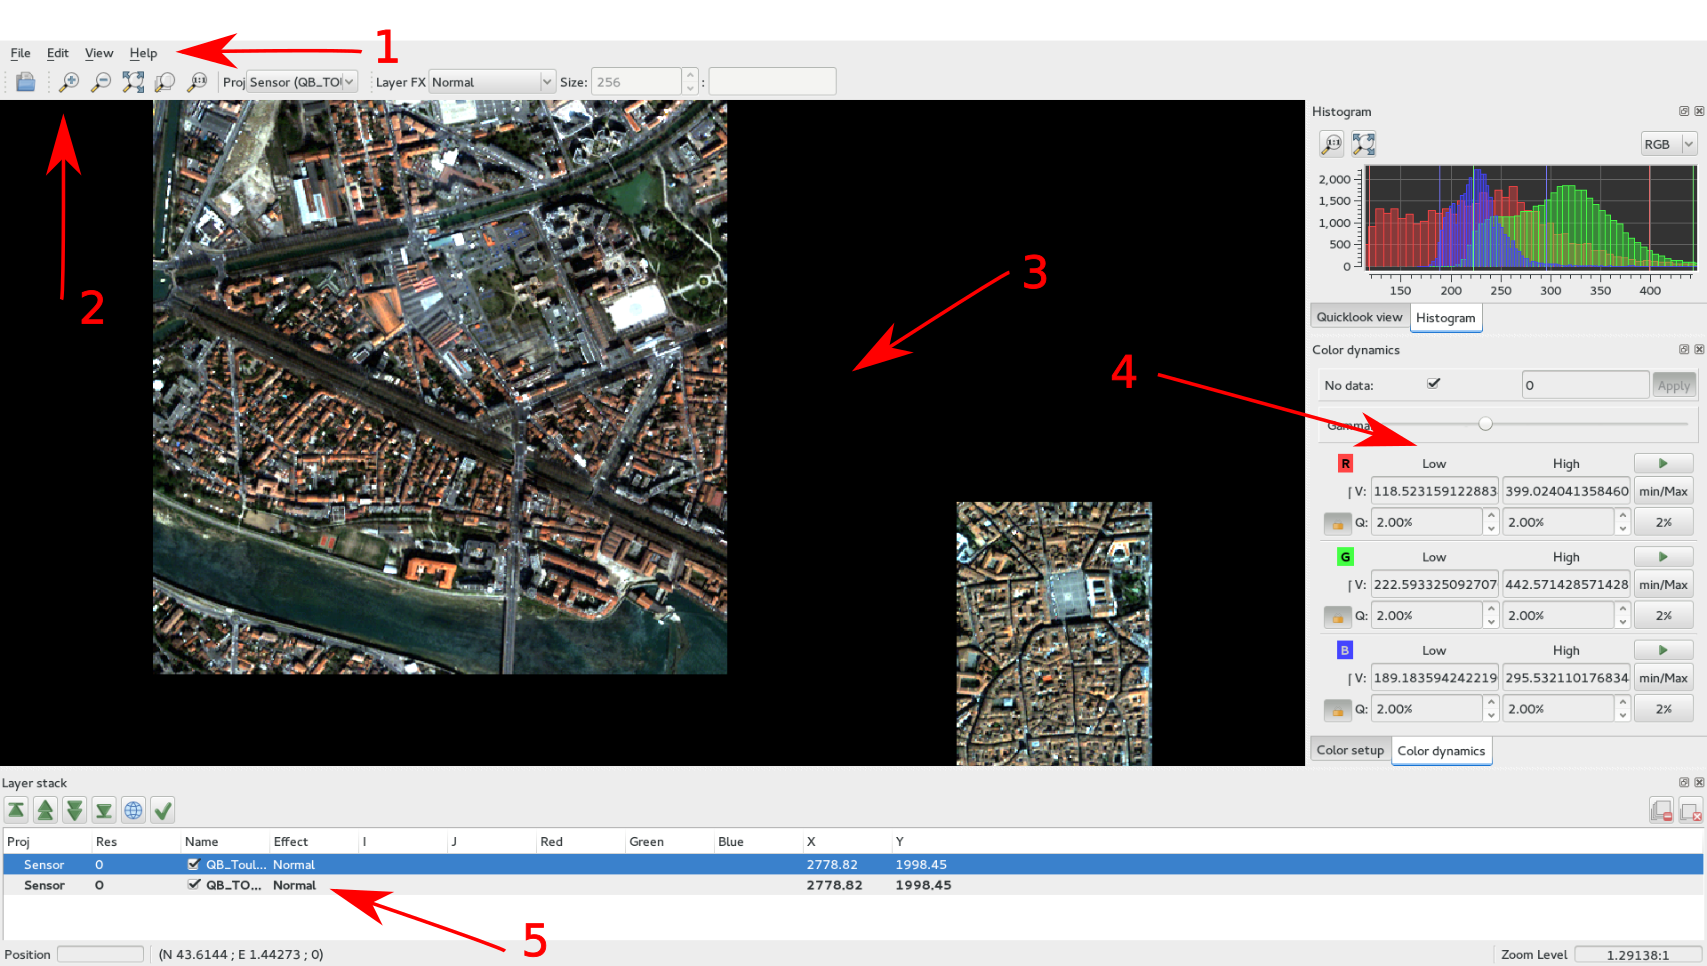
\includegraphics[width=0.95\textwidth]{../Art/MonteverdiImages/gui.png}
  \itkcaption[Monteverdi main window]{\mont's main window.}
  \label{fig:mongui}
\end{figure}

This is \mont's main window (figure ~\ref{fig:mongui}) where the
different functionalities are reachable:

\begin{itemize}
\item 1. Main menu
\item 2. Top toolbar
\item 3. Image displaying
\item 4. Right side dock
\item 5. Stack layer 
\end{itemize}

\subsection{Main menu}
The main menu is made up of four items.
The main one is the File item, from which you can : open a image, load the otb applications, and finally quit \mont.
The Edit item lets the user change his/her preferences. The view item is intended to let the user display or hide different parts of the main window.
Finally, the Help item lets the user know the 'About' information of the software, and also can display an useful keymap.

\subsection{Top toolbar}
The top toolbar is made up of ten icons; from left to right:
\begin{itemize}
\item 1st : open one or more image(s)
\item 2nd : zoom in
\item 3rd : zoom out
\item 4th : zoom to full extent
\item 5th : zoom to layer extent
\item 6th : zoom to full resolution
\item 7th : gives/changes the current projection, used as reference of the view 
\item 8th : selects the effect to be applied to the selected layer : chessboard, local constrast, local translucency, normal, spectral angle, swipe (horizontal and vertical)
\item 9th : a parameter used for the following effects : chessboard, local contrast, local translucency, spectral angle
\item 10th : a parameter used for the following effects :  local constrast, spectral angle
\end{itemize}

\subsection{Image displaying}
This part of the main window is intented to display the images loaded by the user.
There are many nice keyboard shortcuts or mouse tricks that let the user have a better experience in navigating throughout the loaded images.
These shortcuts and tricks are given within the Help item of the main menu, by clicking Keymap; here is a short list of the most useful ones :

The classical ones:
\begin{itemize}
\item CTRL+O = Open file(s)
\item CTRL+Q = Quit application
\end{itemize}

In the image displaying part:
\begin{itemize}
\item Mouse drag = Scroll view
\item CTRL+Mouse drag = Quick scroll view (rending is done after releasing CTRL key)
\item CTRL+Mouse wheel = Zoom in out
\item + or - = Zoom in out
\end{itemize}

In the layer stack part:
\begin{itemize}
\item SHIFT+Page Up = Move layer to top of stack
\item SHIFT+Page Down = Move layer to bottom of stack
\item Delete = Delete selected layer
\item SHIFT+Delete = Delete all layers
\end{itemize}


\subsection{Right side dock}
The dock on the right side is divided into four tabs : 
\begin{itemize}
\item Quicklook : gives the user a degraded view of the whole extent, letting him/her easily select the area to be displayed 
\item Histogram : gives the user information about the value distribution of the selected channels. By clicking the mouse's left button, user can sample their values.
\item Color Setup : lets the user map the image channels to the RGB channels. Also lets him/her set the alpha parameter (translucency).
\item Color dynamics : lets the user change the displaying dynamics of a selected image. For each RGB channel (each mapped to an image channel), the user can decide how the pixel range of a selected image will be shortcut before being rescaled to 0-255 : either by setting the extremal values, or by setting the extremal quantiles.
\end{itemize}

Each tab is represented by the figures below (~\ref{fig:quicklook} ~\ref{fig:histo} ~\ref{fig:colorset} ~\ref{fig:coldyn}).

\begin{figure}[!h] 
  \center
  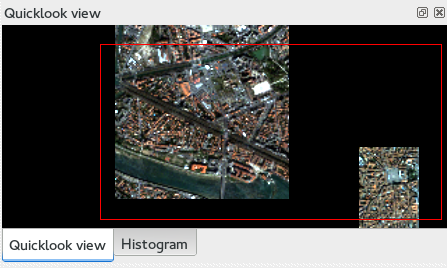
\includegraphics[width=0.6\textwidth]{../Art/MonteverdiImages/quicklook.png}
  \itkcaption[Monteverdi quicklook tab]{Quicklook tab.}
  \label{fig:quicklook}
\end{figure}

\begin{figure}[!h] 
  \center
  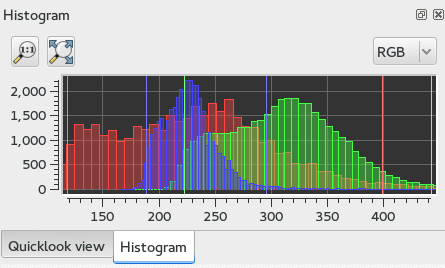
\includegraphics[width=0.6\textwidth]{../Art/MonteverdiImages/histo.png}
  \itkcaption[Monteverdi histogram tab]{Histogram tab.}
  \label{fig:histo}
\end{figure}

\begin{figure}[!h] 
  \center
  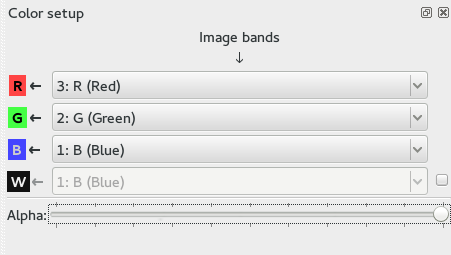
\includegraphics[width=0.6\textwidth]{../Art/MonteverdiImages/colset.png}
  \itkcaption[Monteverdi color setup tab]{Color setup tab.}
  \label{fig:colorset}
\end{figure}

\begin{figure}[!h] 
  \center
  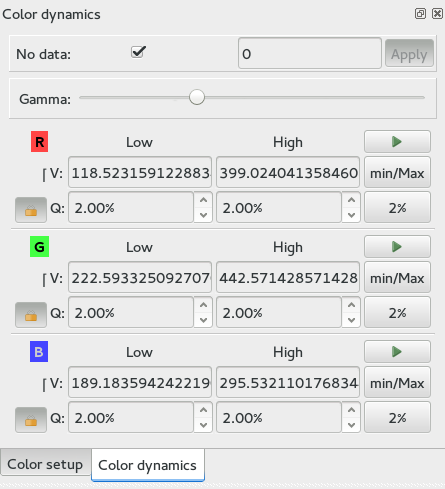
\includegraphics[width=0.6\textwidth]{../Art/MonteverdiImages/coldyn.png}
  \itkcaption[Monteverdi color dyn tab]{Color dynamics tab.}
  \label{fig:coldyn}
\end{figure}


\subsection{Layer stack}

The layer stack is made up of one list of layers located beneath six icons.
The list of layers gives the user some information about the loaded images:
projection, resolution (if available), name, and effect applied to the images (see top toolbar subsection).
If the user moves the mouse over the displayed images, he/she will get more information:

\begin{itemize}
\item (i,j) : pixel index
\item (Red Green Blue) : original image pixel values from channel mapped to the RGB ones.
\item (X,Y) : pixel position
\end{itemize}

Concerning the six icons, from left to right:
\begin{itemize}
\item 1st : moves the selected layer to the top of the stack
\item 2nd : moves the selected layer up within the stack
\item 3rd : moves the selected layer down within the stack
\item 4th : moves the selected layer to the bottom of the stack
\item 5th : use selected layer as projection reference
\item 6th : applies all display settings (color-setup, color-dynamics, shader and so forth) of selected layer to all other layers
\end{itemize}

The layer stack is represented in the figure below (~\ref{fig:layerstack}) :
\begin{figure}[!h] 
  \center
  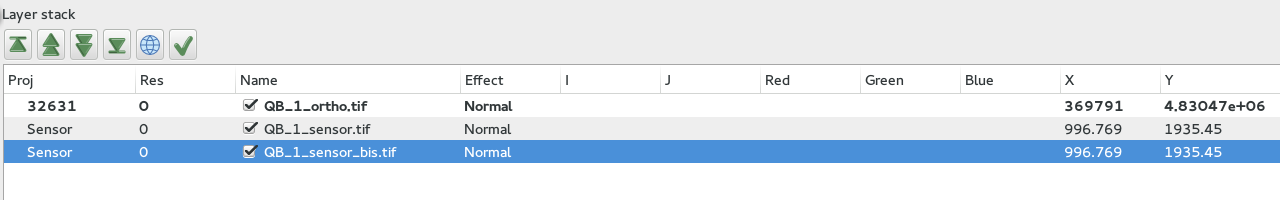
\includegraphics[width=0.95\textwidth]{../Art/MonteverdiImages/layerstack.png}
  \itkcaption[Monteverdi layerstack]{Layer stack.}
  \label{fig:layerstack}
\end{figure}


\section{Examples}\label{sec:monexamples}

With \mont, it is also possible to interactively load otb-applications and use them to process images.
For that purpose, the user just has to load otb-applications by clicking on the Main menu, File/Load OTB-Applications (or by simply using the shorcut CTRL+A).
The figure below (~\ref{fig:applications}) represents the otb-applications loading window. The applications are arranged in thematic functionalities; the user can also quickly find the wanted application by typing its name in the dedicated field
at the top of the loading window.


\begin{figure}[!h] 
  \center
  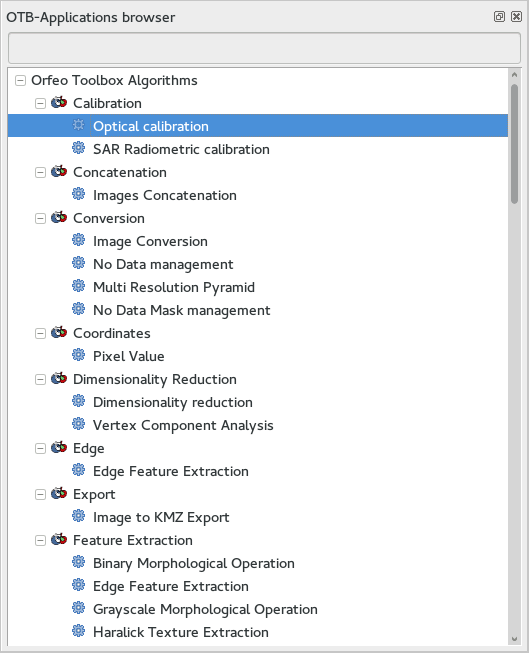
\includegraphics[width=0.6\textwidth]{../Art/MonteverdiImages/applications.png}
  \itkcaption[Monteverdi app]{Applications window.}
  \label{fig:applications}
\end{figure}


\subsection{Optical calibration}\label{ssec:monoptical}

In order to perform an optical calibration, launch the Optical calibration application (shortcut CTRL+A). 
We are going to use this application to perform a TOA (Top Of Atmosphere) conversion, which consists in converting the DN pixel values into spectral radiance (in W/m2/steradians/micrometers).
Once the application is launched, the user must fill the required fields in
(in, out, gainbias.txt -gain and bias values in a txt file-, solarillumination.txt -solar illumination values in watt/m2/micron for each band in a txt file-, and so on... refer to the documentation of the application).
\begin{itemize}
\item Note : if OTB (on which is based \mont) is able to parse the metadata of the image to be calibrated, then some of the fields will be automatically filled in.
\end{itemize}

In the figure below (~\ref{fig:OC}), by taking a look at the layer stack, one can notice that the values of the calibrated image are now expressed in spectral radiance.


\begin{figure}[!h] 
  \center
  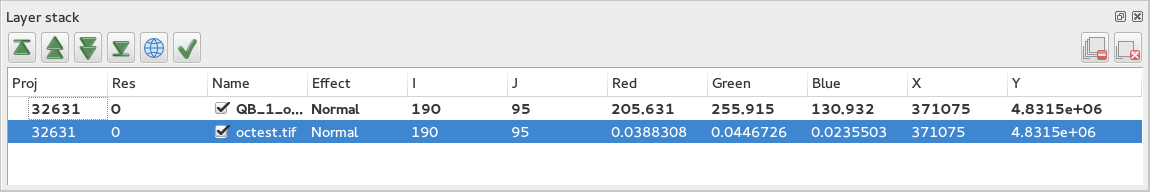
\includegraphics[width=0.6\textwidth]{../Art/MonteverdiImages/OC.png}
  \itkcaption[Monteverdi OC]{Before and after calibration.}
  \label{fig:OC}
\end{figure}



\subsection{BandMath}\label{ssec:monbandmath}

BandMath application is intented to apply mathematical operations on pixels (launch it with shortcut CTRL+A). In this example, we are going to use this application to change the dynamics of an image,
and check the result by looking at histogram tab, in the right side dock. The formula used is the following : im1b1*1000.
In the figures below (~\ref{fig:BM1}, ~\ref{fig:BM2}), one can notice that the mode of the distribution is located at position 356.0935, whereas in the transformed image,
the mode is located at position 354737.1454, that's to say 1000 times farther away approximatelly (the cursors weren't placed exactly at the same position during screenshots).


\begin{figure}[!h] 
  \center
  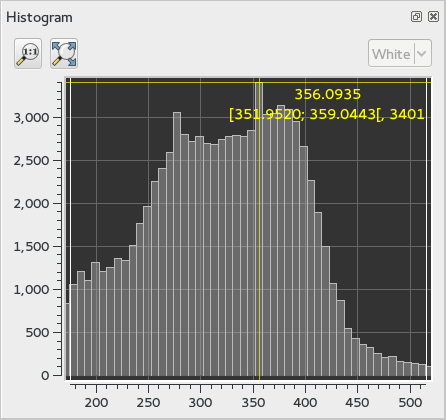
\includegraphics[width=0.6\textwidth]{../Art/MonteverdiImages/BM1.png}
  \itkcaption[Monteverdi BM1]{Before applying BandMath.}
  \label{fig:BM1}
\end{figure}

\begin{figure}[!h] 
  \center
  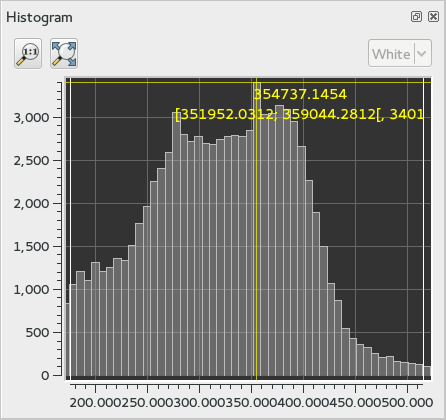
\includegraphics[width=0.6\textwidth]{../Art/MonteverdiImages/BM2.png}
  \itkcaption[Monteverdi BM2]{After applying BandMath.}
  \label{fig:BM2}
\end{figure}


\subsection{Segmentation}\label{ssec:monseg}

Now, let's use the segmentation application (launch it with shortcut CTRL+A). 
We let the user take a look at the application's documentation; let's simply say that as we wish we could display the segmentation with \mont,
we must tell the application to output the segmentation in raster format. Thus, the value of the mode option must be set to raster.
The two following figures (~\ref{fig:seg1} and ~\ref{fig:seg2}) show the original image and the labels image.

\begin{figure}[!h] 
  \center
  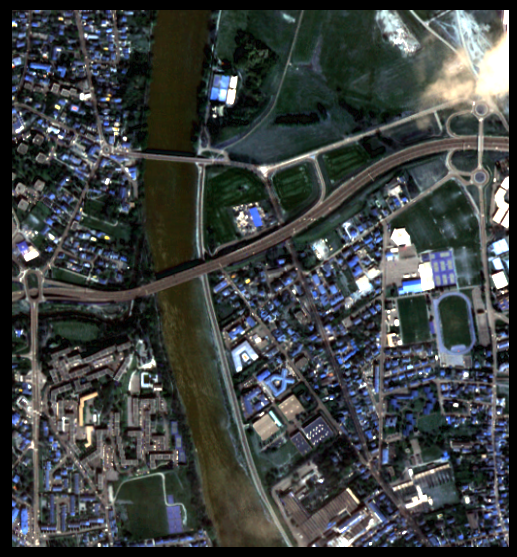
\includegraphics[width=0.6\textwidth]{../Art/MonteverdiImages/seg1.png}
  \itkcaption[Monteverdi seg1]{Original image.}
  \label{fig:seg1}
\end{figure}

\begin{figure}[!h] 
  \center
  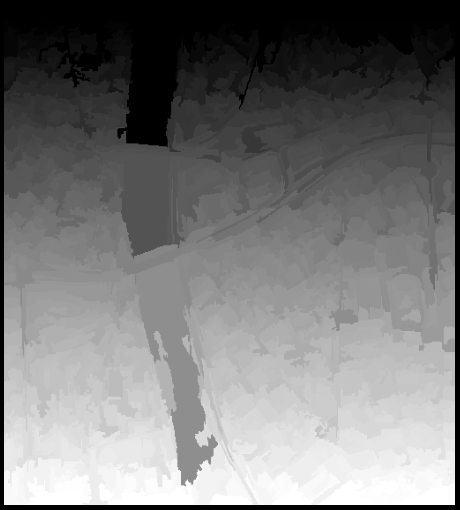
\includegraphics[width=0.6\textwidth]{../Art/MonteverdiImages/seg2.png}
  \itkcaption[Monteverdi seg2]{Labels image.}
  \label{fig:seg2}
\end{figure}

Gray colors aren't very convenient for visualizing a segmentation. That's why we are going to use another application, the ColorMapping one (launch it with the sortcut CTRL+A as usual).
There are many ways to use this application (see the documentation for more details). We wish we could colour the segmentation so that color difference between adjacent regions is maximized.
For this purpose, we can use the method optimal (set the value of this option to optimal). The figure below (~\ref{fig:seg3}) shows the result of such colorization.

\begin{figure}[!h] 
  \center
  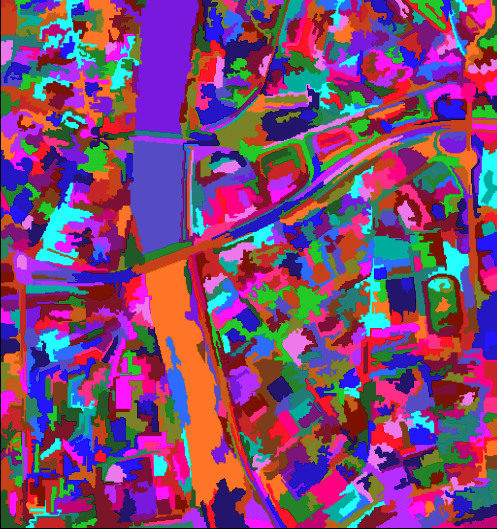
\includegraphics[width=0.6\textwidth]{../Art/MonteverdiImages/seg3.png}
  \itkcaption[Monteverdi seg3]{Optimally colored labels image.}
  \label{fig:seg3}
\end{figure}

Now it should be nice to superimpose this colorization with the original image to assess the quality of the segmentation.
\mont provides the user a very simple way to do it. Once the two images are loaded in \mont and that the original image is placed on the top of the stack, 
the user just has to select the translucency layer effect and set the size of the exploration circle to convenience.
The figure below (~\ref{fig:seg4}) shows the result of such colorization. We encourage the reader to test the other layer effects.

\begin{figure}[!h] 
  \center
  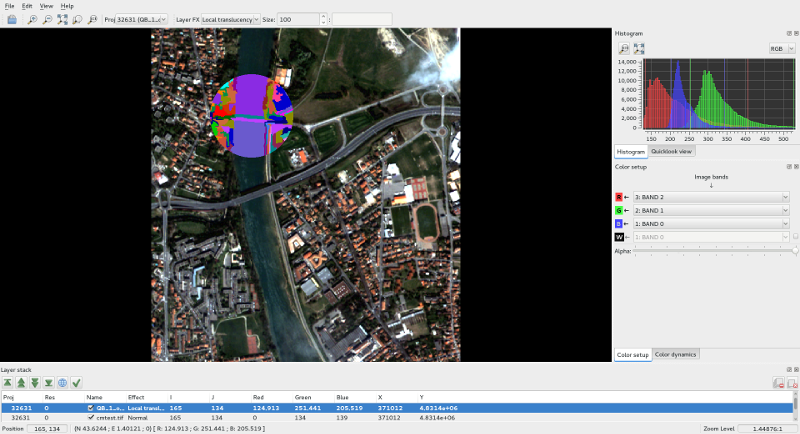
\includegraphics[width=0.95\textwidth]{../Art/MonteverdiImages/seg4.png}
  \itkcaption[Monteverdi seg4]{Nice layer effect, local translucency, to ease the comparison between the original image and its segmentation.}
  \label{fig:seg4}
\end{figure}

\subsection{Polarimetry}\label{ssec:monpolar}
In this example, we are going to use three applications : 
\begin{itemize}
\item the first one is SARDecompositions. This application is used to compute the HaA decomposition. It takes as inputs three complex channels from bands HH HV and VV.
\item the second one is SplitImage. Indeed, the previous application had produced an output image made up of three channels, H a and A, and we wish to focuse on the H parameter (entropy). 
So we let this application split this image into three one-band-images.
\item the last one is ColorMapping. The entropy image has values ranging from 0 to 1, and they can be easily displayed by \mont. But since we have a nice visualizing tool in hand, we wish we could go a little bit further.
Here comes the application ColorMapping. It is going to be used with the following parameter settings:
\begin{itemize}
\item method = continous. This parameters tells the application to use a gradient of colors to represent the entropy image.
\item method.continuous.lut = hot. We specify here the kind of gradient to be used : low values in black, high ones in white, and intermediate ones in red/orange/yellow...
\item method.continuous.min = 0 and method.continuous.max = 1. Here, the gradient of colors must be adjusted to the dynamic of the entropy image (note: it is theoretically known that in HaA decomposition, H ranges from 0 to 1. Generally speaking, the histogram of \mont can also be used for this purpose).
\end{itemize}
\end{itemize}

In the figure below (~\ref{fig:pol1}), we show the obtained result, with the local contrast layer effect.

\begin{figure}[!h] 
  \center
  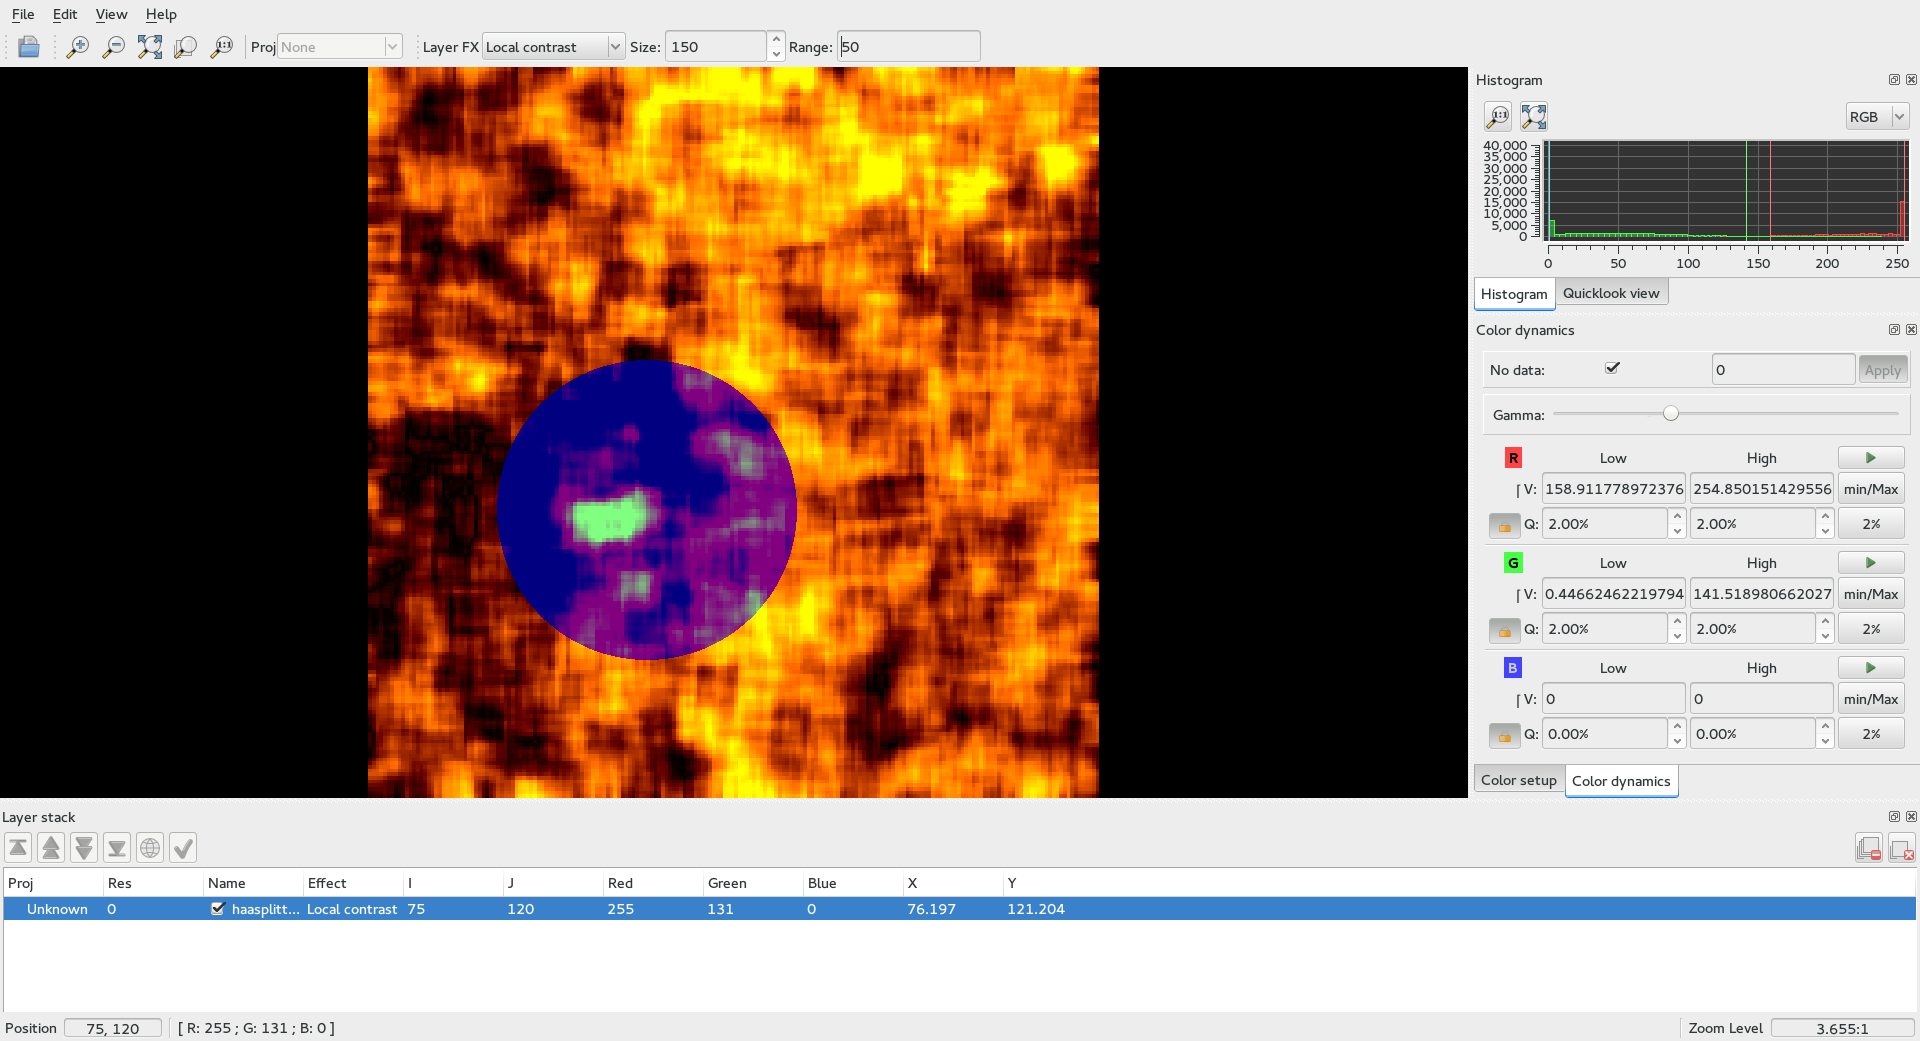
\includegraphics[width=0.95\textwidth]{../Art/MonteverdiImages/pol1.png}
  \itkcaption[Monteverdi pol1]{Entropy image represented in temperature colors; layer effet : local constrast.}
  \label{fig:pol1}
\end{figure}


\subsection{Pansharpening}\label{ssec:monpansh}
Finally, let's try a last example with the Pansharpening application (launch it with shortcut CTRL+A).
The fields are quite easy to fill in : this application needs a panchromatic image, a XS image, and an output image.
These images are represented in the figures below (~\ref{fig:ps1}, ~\ref{fig:ps2} and ~\ref{fig:ps3}):

\begin{figure}[!h] 
  \center
  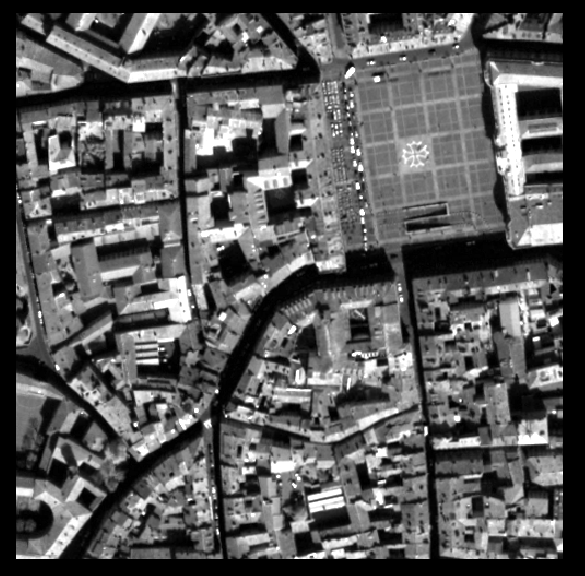
\includegraphics[width=0.6\textwidth]{../Art/MonteverdiImages/ps1.png}
  \itkcaption[Monteverdi ps1]{Panchromatic image.}
  \label{fig:ps1}
\end{figure}

\begin{figure}[!h] 
  \center
  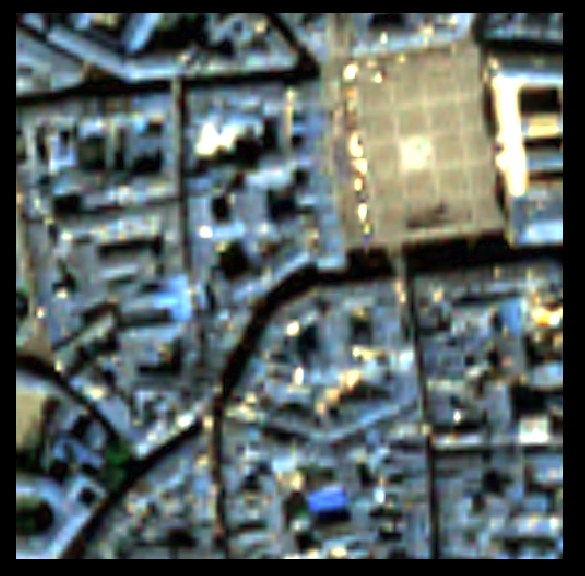
\includegraphics[width=0.6\textwidth]{../Art/MonteverdiImages/ps2.png}
  \itkcaption[Monteverdi ps2]{XS image.}
  \label{fig:ps2}
\end{figure}

\begin{figure}[!h] 
  \center
  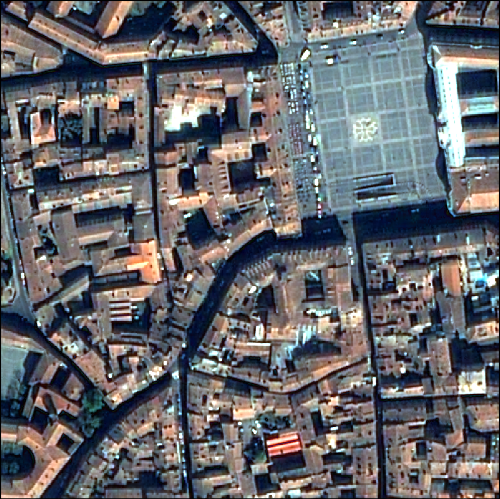
\includegraphics[width=0.6\textwidth]{../Art/MonteverdiImages/ps3.png}
  \itkcaption[Monteverdi ps3]{Pansharpened image.}
  \label{fig:ps3}
\end{figure}

Now, in order to inspect the result properly, these three images are loaded in \mont.
The pansharpened image is placed to the top of the stack layer, and different layer effects are applied to it :
\begin{itemize}
\item in figure ~\ref{fig:ps4} : chessboard effect, to compare the result with the XS image.
\item in figure ~\ref{fig:ps5} : translucency effect, to compare the result with the panchromatic image.
\end{itemize}

\begin{figure}[!h] 
  \center
  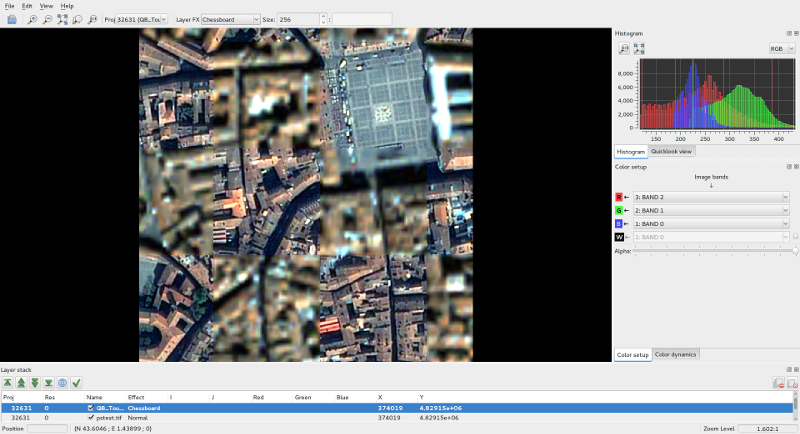
\includegraphics[width=0.95\textwidth]{../Art/MonteverdiImages/ps4.png}
  \itkcaption[Monteverdi ps4]{XS image with panchromatic image; chessboard layer effect.}
  \label{fig:ps4}
\end{figure}

\begin{figure}[!h] 
  \center
  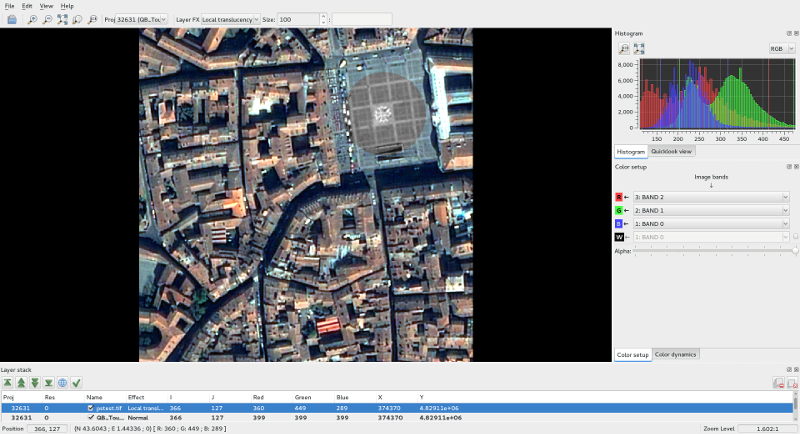
\includegraphics[width=0.95\textwidth]{../Art/MonteverdiImages/ps5.png}
  \itkcaption[Monteverdi ps5]{Pansharpened image with panchromatic image; translucency layer effect.}
  \label{fig:ps5}
\end{figure}





\chapter{Recipes}\label{chap:recipes}

This chapter presents guideline to perform various remote sensing and
image processing tasks with either \app, \mont or both. Its goal is
not to be exhaustive, but rather to help the non-developper user to
get familiar with these two packages, so that he can use and explore
them for his future needs.

\section{Optical pre-processing}\label{sec:optpreproc}

This section present various pre-processing tasks that can be done
using \app or \mont. The tasks are presented in their classical order
in which they can be chained to obtain a calibrated, pan-sharpened 

\subsection{Optical radiometric calibration}\label{ssec:optcal}

In remote sensing imagery, pixel values are called DN (for Digital
Numbers) and can not be physically interpreted and compared: they are
influenced by various factors such as the amount of light flowing
trough the sensor, the gain of the detectors and the analogic to
numeric converter.

Depending on the season, the light and atmospheric conditions, to
position of the sun or the sensor internal parameters, these DN can
drastically change for a given pixel (apart from any ground change
effects). Moreover, these effect are not uniform over the spectrum:
for instance aerosol amount and type has usually more impact on the
blue channel.

Therefore, it is necessary to calibrate the pixel values before any
physical interpretation is made out of them. In particular, this
processing is mandatory before any comparison of pixel spectrum
between several images (from the same sensor), and to train a
classifier without dependence to the atmospheric conditions at the
acquisition time.

Calibrated values are called surface reflectivity, which is a ratio
denoting the fraction of light that is reflected by the underlying
surface in the given spectral range. As such, its values lie in the
range $[0,1]$. For convenience, images are often stored in thousandth
of reflectivity, so that they can be encoded with an integer type.
Two levels of calibration are usually distinguished:

\begin{itemize}
\item The first level is called \emph{Top Of Atmosphere (TOA)}
  reflectivity. It takes into account the sensor gain, sensor spectral
  response and the solar illumination.
\item The second level is called \emph{Top Of Canopy (TOC)}
  reflectivity. In addition to sensor gain and solar illumination, it
  takes into account the optical thickness of the atmosphere, the
  atmospheric pressure, the water vapor amount, the ozone amount, as
  well as the composition and amount of aerosol gasses.
\end{itemize}

This transformation can be done either with \app or with
\mont. Sensor-related parameters such as gain, date, spectral
sensitivity and sensor position are seamlessly read from the image
metadata. Atmospheric parameters can be tuned by the user. Supported
sensors are :
\begin{itemize}
\item SPOT5,
\item QuickBird,
\item Ikonos,
\item WorldView1,
\item WorldView2,
\item Formosat.
\end{itemize}

\subsubsection{Optical calibration with \app}

The \application{otbOpticalCalibration-cli} application from \app
allows to perform command-line optical calibration. The mandatory
parameters are the input and output images and the level of
calibration (either TOA or TOC). All other parameters are
optional. The output images are expressed in thousandth of
reflectivity using a 16 bits unsigned integer type.

A basic TOA calibration task can be performed with the following command :

\begin{verbatim}
otbOpticalCalibration-cli -in  input_image -out output_image -level TOA
\end{verbatim}

A basic TOC calibration task can be performed with the following command :

\begin{verbatim}
otbOpticalCalibration-cli -in  input_image -out output_image -level TOC
\end{verbatim}

\subsubsection{Optical calibration with \mont}

These transformations can also be done in \mont.

The 6S model needs atmospheric parameters to be able to compute
radiative terms to estimate the atmoshperic contributions on the input
signal. Default parameters are available in the module.  For
atmospheric parameters, it is possible to indicate AERONET file. The
AERONET (AErosol RObotic NETwork) program is a federation of
ground-based remote sensing aerosol networks established by NASA and
PHOTONS (Univ. of Lille 1, CNES, and CNRS-INSU) and is greatly
expanded by collaborators from national agencies, institutes,
universities, individual scientists, and partners. The program
provides accessible public domain database of aerosol optical,
mircrophysical and radiative properties.

The module produce four outputs:

\begin{itemize}
\item Luminance image
\item TOA reflectance image
\item TOC reflectance image
\item Difference TOA-TOC image which allows to get the estimation of atmospheric contribution
\end{itemize}

\begin{figure}
  \center
  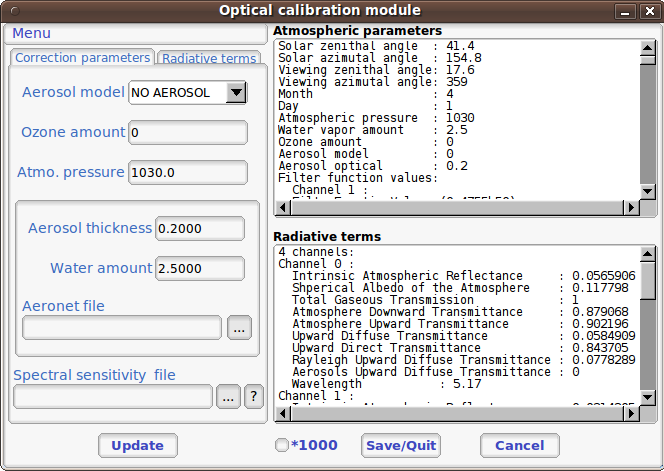
\includegraphics[width=0.6\textwidth]{../Art/MonteverdiImages/monteverdi_optical_calibration.png}
  \itkcaption[GUI of the optical calibration module based on the 6S model]{Optical calibration module.}
  \label{fig:opticalcalibration}
\end{figure}


\begin{figure}
  \center
  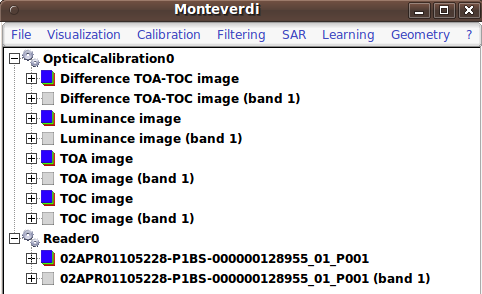
\includegraphics[width=0.6\textwidth]{../Art/MonteverdiImages/monteverdi_optical_calibration_outputs.png}
  \itkcaption[Output of the optical calibration module]{Optical calibration module's outputs.}
  \label{fig:opticalcalibrationoutput}
\end{figure}

\subsection{Pan-sharpening}\label{ssec:pxs}

Because of physical constrains on the sensor design, it is difficult
to achieve high spatial and spectral resolution at the same time : a
better spatial resolution means a smaller detector, which in turns
means lesser optical flow on the detector surface. On the contrary,
spectral bands are obtained through filters applied on the detector
surface, that lowers the optical flow, so that it is necessary to
increase the detector size to achieve an acceptable signal to noise
ratio.

For these reasons, many high resolution satellite payload are composed
of two sets of detectors, which in turns delivers two different kind
of images :

\begin{itemize}
\item The multi-spectral (XS) image, composed of 3 to 8 spectral bands
  containing usually blue, green, red and near infra-red bands at a
  given resolution (usually from 2.8 meters to 2 meters).
\item The panchromatic (PAN) image, which is a grayscale image acquired by a
  detector covering a wider part of the light spectrum, which allows
  to increase the optical flow and thus to reduce pixel
  size. Therefore, resolution of the panchromatic image is usually
  around 4 times lower than the resolution of the multi-spectral image
  (from 46 centimeters to 70 centimeters).
\end{itemize}

It is very frequent that those two images are delivered side by side
by data providers. Such a dataset is called a bundle. A very common
remote sensing processing is to fuse the panchromatic image with the
multi-spectral one so as to get an image combining the spatial
resolution of the panchromatic image with the spectral richness of the
multi-spectral image. This operation is called pan-sharpening.

This fusion operation requires two different steps :
\begin{enumerate}
\item The multi-spectral (XS) image is zoomed and registered to the
  panchromatic image,
\item A pixel-by-pixel fusion operator is applied to the co-registered
  pixels of the multi-spectral and panchromatic image to obtain the
  fused pixels.
\end{enumerate}

Using either an application from \app or modules from \mont, it is
possible to perform both steps in a raw, or step-by-step fusion, as
described in the above sections.

\subsubsection{Pan-sharpening with \app}

The \application{otbBundleToPerfectSensor-cli} application allows to
perform both steps in a raw. Seamless sensor modelling is used to
perform zooming and registration of the multi-spectral image on the
panchromatic image. Then, a simple pan-sharpening is applied,
according to the following formula:

\begin{equation}
PXS(i,j) = \frac{PAN(i,j)}{PAN_{smooth}(i,j)} \cdot XS(i,j)
\end{equation}

Where $i$ and $j$ are pixels indices, $PAN$ is the panchromatic image,
$XS$ is the multi-spectral image and $PAN_{smooth}$ is the
panchromatic image smoothed with a kernel to fit the multi-spectral
image scale.

Here is a simple example of how to use the
\application{otbBundleToPerfectSensor-cli} application:

\begin{verbatim}
otbBundleToPerfectSensor-cli -inP pan_image -inXS xs_image -out output_image
\end{verbatim}

There are two more optional parameters that can be useful for this
tool:
\begin{itemize}
\item The \verb?-dem? option allows to specify a directory containing DEM
  formatted for OTB (see section~\ref{ssec:dem}). Since registration
  and zooming of the multi-spectral image is performed using
  sensor-models, it may happen that the registration is not perfect in
  case of landscape with high elevation variation. Using a DEM in this
  case allows to get better registration (see \ref{ssec:registration}
  to learn about how to lower registration error).
\item The \verb?-lmSpacing? option allows to specify the step of the
  registration grid between the multi-spectral image and panchromatic
  image. This is expressed in amount of panchromatic pixels. A lower
  value gives a more precise registration but implies more computation
  with the sensor models, and thus increase the computation
  time. Default value is 10 pixels, which gives sufficient precision
  in most of the cases.
\end{itemize}

Pan-sharpening is a quite heavy processing requiring a lot of system
resource. The \verb?-ram? option allows you to limit the amount of memory
available for the computation, and to avoid overloading your
computer. Increasing the available amount of RAM may also result in
better computation time, seems it optimises the use of the system
resources. Default value is 256 Mb.


\subsubsection{Pan-sharpening with \mont}

\mont allows to perform step-by-step fusion. The followings screenshots highlight operations needed to perform Pan-Sharpening.

\begin{itemize}
\item Open panchromatic and multispectral images in monteverdi using the \mmod{Open Dataset} module or using the  \verb?-iml? option of the \mont executable.

\item The \mmod{Superimpose} module is used to zoomed and registered
  the multispectral on the panchromatic image. As a result, we get a
  multispectral dataset with the same geographic extension and the
  same resolution as the panchromatic image, cf ~\ref{fig:qbmulsuper}.

\begin{figure}
  \center
  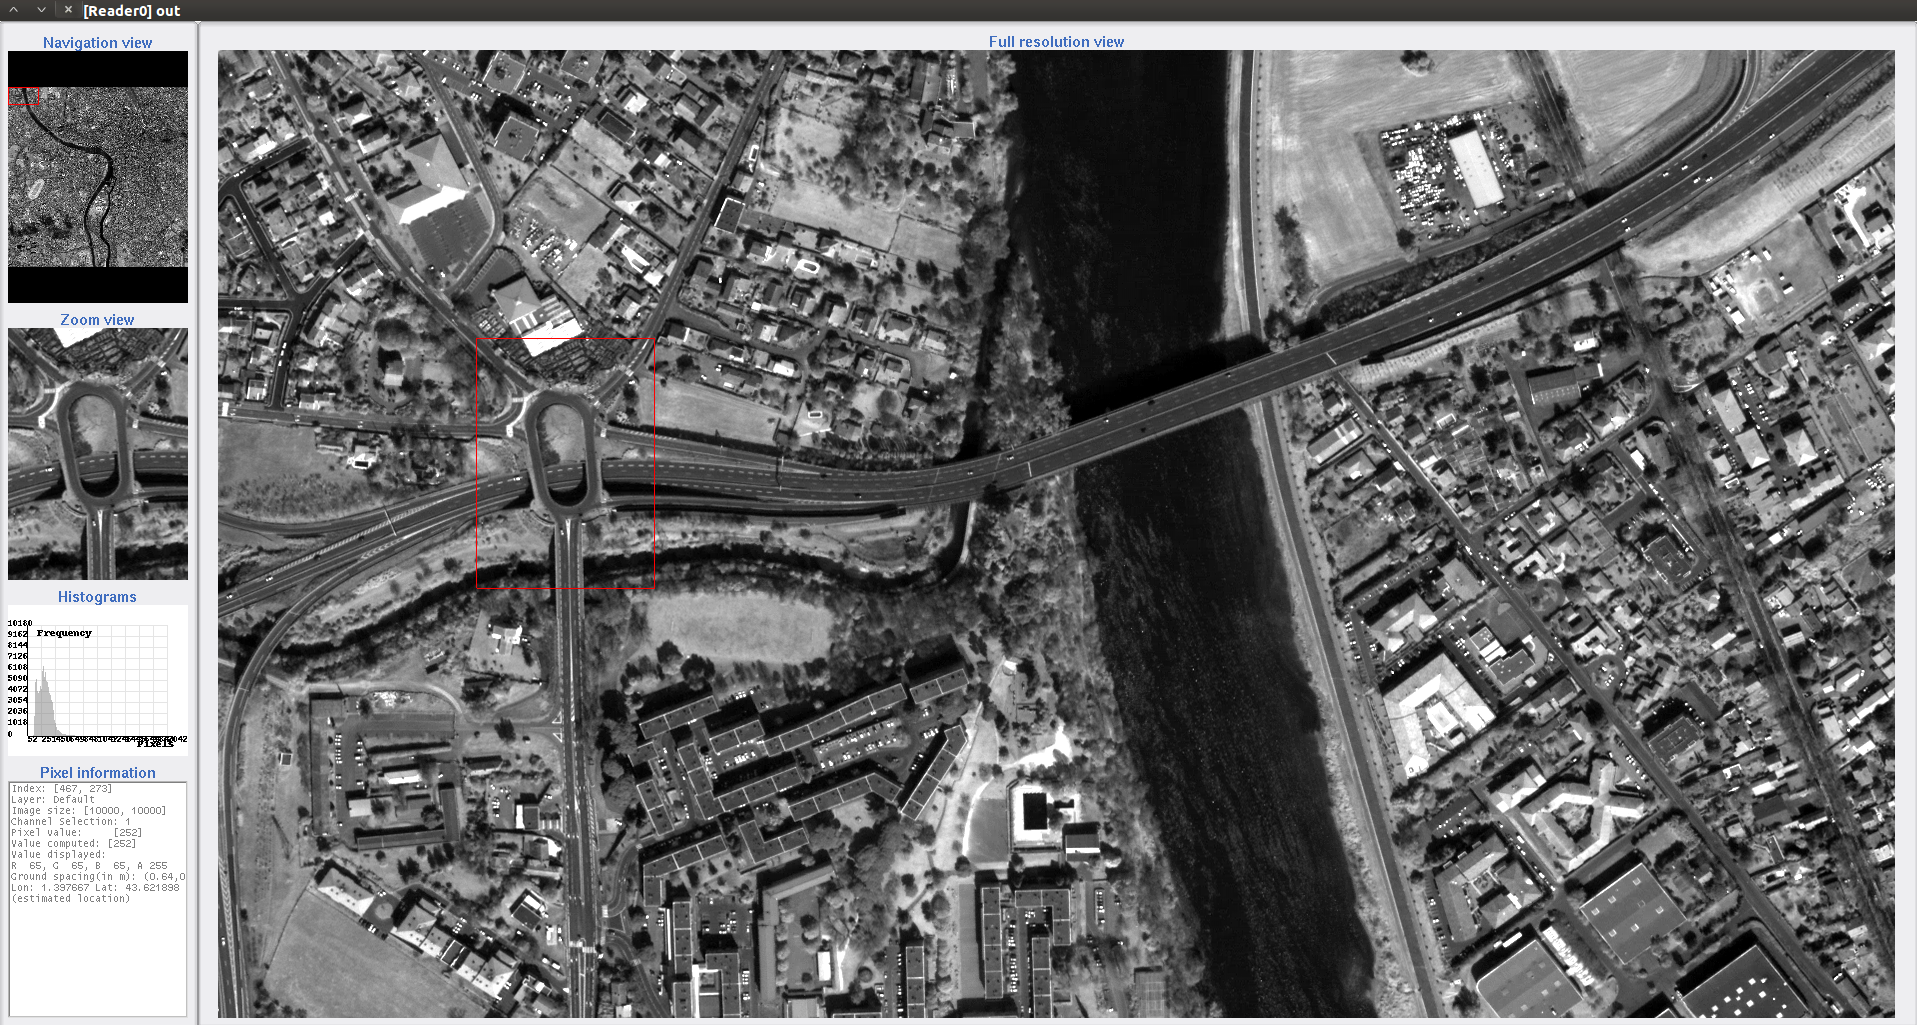
\includegraphics[width=0.45\textwidth]{../Art/MonteverdiImages/monteverdi_QB_PAN_ROI.png}
  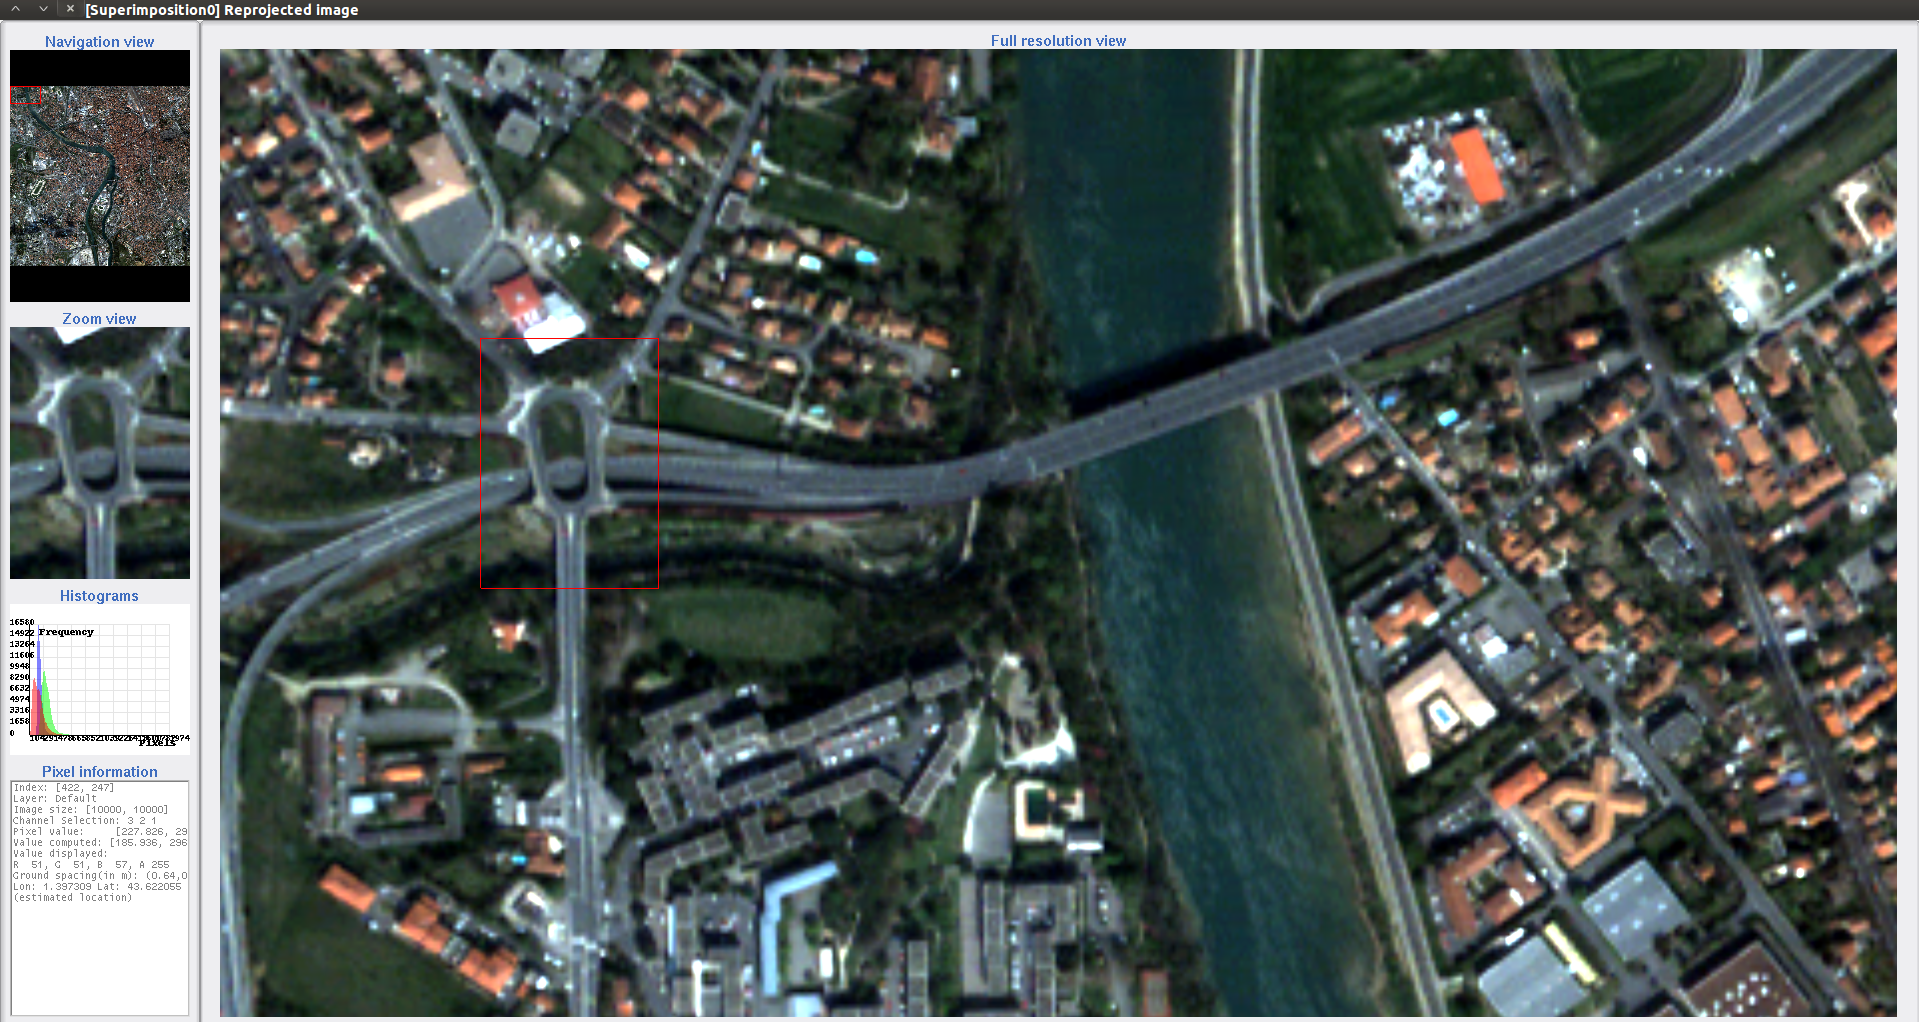
\includegraphics[width=0.45\textwidth]{../Art/MonteverdiImages/monteverdi_QB_MUL_Superimpose.png}
  \itkcaption[Input panchromatic and zoomed and registered multispectral image over it]{Panchromatic and Zoomed and registered Multispectral image.}
  \label{fig:qbmulsuper}
\end{figure}

\item Now the \mmod{Simple RCS pan-sharpening} module can be used using the panchromatic and the multispectral images as inputs. It produces a multispectral image with the same resolution and geographic extension (cf ~\ref{fig:pansharpen}).

\begin{figure}
  \center
  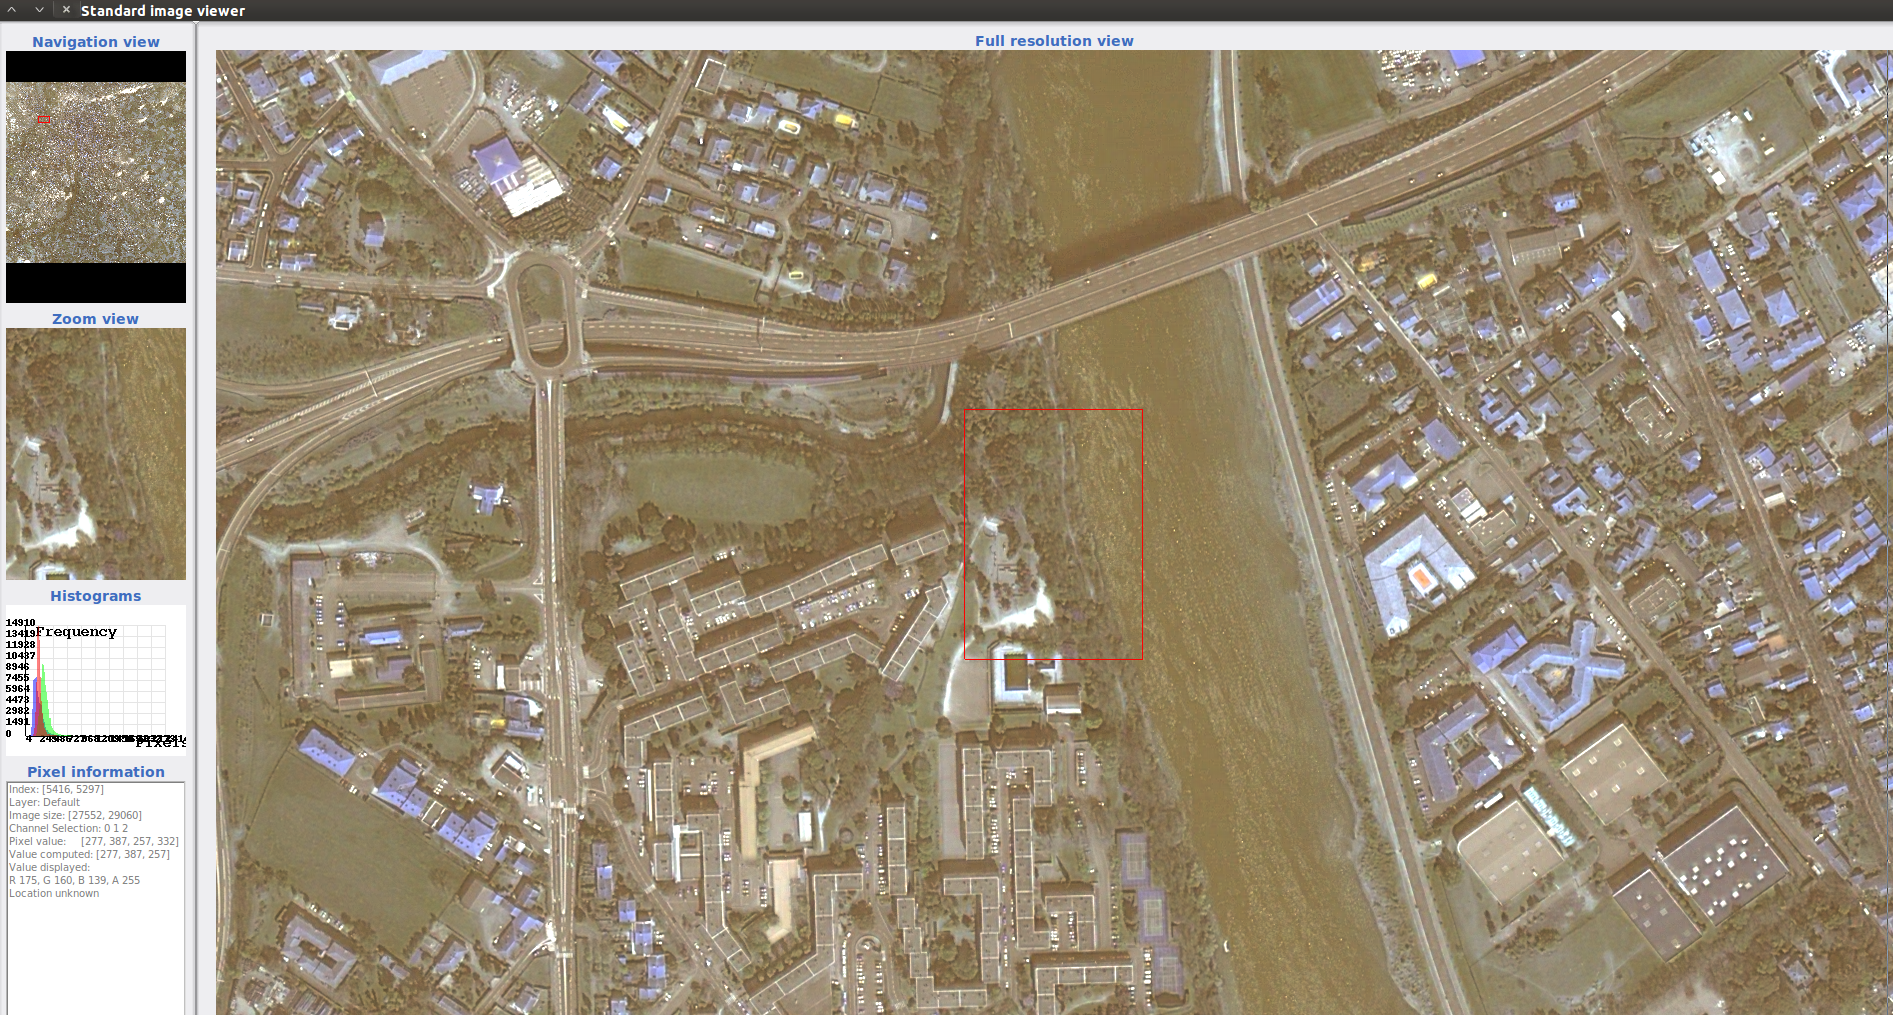
\includegraphics[width=0.6\textwidth]{../Art/MonteverdiImages/monteverdi_QB_XS_pan-sharpened.png}
  \itkcaption[Pan-sharpened image]{Pan-sharpened image using the simple RCS module.}
  \label{fig:pansharpen}
\end{figure}

\end{itemize}


Please also note that since registration and zooming of the
multi-spectral image with the panchromatic image relies on sensor
modelling, this tool will work only for images whose sensor models is
available in \otb (see section~\ref{ssec:ortho} for a detailed
list). It will also work with ortho-ready products in cartographic
projection.

\subsection{Digital Elevation Model management}\label{ssec:dem}

A Digital Elevation Model (DEM) is an georeferenced image (collection
of images) of the elevation. DEM are useful for tasks involving sensor
to ground and ground to sensor coordinate transforms like
ortho-rectification (see section~\ref{ssec:ortho}). In facts, these
transforms need to find the intersection between the line of sight of
the sensor and the earth geoid. If a simple spheroid is used as the
earth model, potentially high localisation errors can be made in areas
where elevation is high or perturbed. Of course, DEM accuracy and
resolution have a great impact on the precision of these transforms.

There exists two main available DEM free of charges with worldwide
cover, which are both delivered as 1-by-1 tiles:
\begin{itemize}
\item \href{http://www2.jpl.nasa.gov/srtm/}{The Shuttle Radar
  topographic Mission (SRTM)} is a 90 meters resolution DEM, obtained
  by radar interferometry during a campaign of the Endeavour space
  shuttle from NASA in 2000. The 
\item The \href{http://www.ersdac.or.jp/GDEM/E/2.html}{Advanced
  Spaceborne Thermal Emission and Reflection Radiometer (ASTER)} is a
  30 meters resolution DEM obtained by stereoscopic processing of the
  archive of the ASTER instrument.
\end{itemize}

The \otb suite relies on \ossim capabilities for sensor modelling and
DEM handling. Tiles of a given DEM are supposed to be located within a
single directory. Whenever some application from \app or module from
\mont requires a DEM, there is an option or a field to set the DEM
directory.

\subsubsection{Making DEM files usable in \otb suite using \app}

Georeferenced files containing elevation data (including file from
SRTM and ASTER) need to be converted to a specific file format before
being compatible with \ossim and \otb. The
\application{otbDEMConvert-cli} application allows to perform this
conversion with the following command:

\begin{verbatim}
otbDEMConvert-cli -in input_image -out output_image
\end{verbatim}

The output image can then be placed in the directory containing DEM
files.

\subsubsection{Extract the DEM image corresponding to your image using
  \mont}


\subsection{Ortho-rectification and map projections}\label{ssec:ortho}

There are several level of products available on the remote sensing
imagery market. The most basic level often provide the geometry of
acquisition (sometimes called the raw geometry). In this case, pixel
coordinates can not be directly used as geographical positions. For
most sensors (but not for all), the different lines corresponds to
different acquisition times and thus different sensor positions, and
different rows correspond to different cells of the detector.

The mapping of a raw image so as to be registered to a cartographic
grid is called ortho-rectification, and consist in inverting the
following effects (at least):
\begin{itemize}
\item In most cases, lines are orthogonal to the sensor trajectory,
 which is not exactly (and in some case not at all) following a
 north-south axis,
\item Depending on the sensor, the line of sight may be different from
  a Nadir (ground position of the sensor), and thus a projective
  warping may appear,
\item The variation of height in the landscape may result in severe
  warping of the image.
\end{itemize}

Moreover, depending on the area of the world the image has been
acquired on, different map projections should be used.

The ortho-rectification process is as follows: once an appropriate map
projection has been defined, a localisation grid is computed to map
pixels from the raw image to the ortho-rectified one. Pixels from the
raw image are then interpolated according to this grid in order to
fill the ortho-rectified pixels.

Ortho-rectification can be performed either with \app or \mont. Sensor
parameters and image meta-data are seamlessly read from the image
files without needing any user interaction, provided that all
auxiliary files are available. The sensor for which \otb
supports ortho-rectification of raw products are the following:
\begin{itemize}
\item SPOT5,
\item Ikonos,
\item Quickbird,
\item GeoEye,
\item WorldView.
\end{itemize}

In addition, GeoTiff and other file format with geographical
information are seamlessly read by OTB, and the ortho-rectification
tools can be used to re-sample these images in another map projection.

\subsubsection{Ortho-rectification with \app}

The \application{otbOrthoRectification-cli} application allows to
perform ortho-recification and map re-projection. The simplest way to
use it is the following:
\begin{verbatim}
otbOrthoRectification-cli -in input_image -out output_image
\end{verbatim}

In this case, the tool will automatically estimates all the necessary
parameters:
\begin{itemize}
\item The map projection is set to UTM (a worldwide map projection)
  and the UTM zone is automatically estimated,
\item The ground sampling distance of the output image is computed to
  fit the image resolution,
\item The region of interest (upper-left corner and size of the image)
  is estimated so as to contain the whole input image extent.
\end{itemize}

In order to use a Digital Elevation Model (see section~\ref{ssec:dem})
for better localisation performances, one can pass the directory
containing the DEM tiles to the application:

\begin{verbatim}
otbOrthoRectification-cli -in input_image -out output_image -dem dem_dir
\end{verbatim}

If one wants to use a different map projection, the \emph{-mapProj}
option may be used (example with \emph{Lambert93} map projection):

\begin{verbatim}

otbOrthoRectification-cli -in input_image -out output_image -dem
dem_dir -mapProj projection parameters

\end{verbatim}

Map projections handled by the application are the following
(parameters should be passed as demonstrated, please note that the
ellipsoid is always WGS84):
\begin{itemize}
\item UTM, emisphere is either north (N) or south (S): \begin{verbatim} -mapProj UTM zone emisphere \end{verbatim}
\item Lambert Conformal Conic: \begin{verbatim}-mapProj LAMBERT std_parallel1 std_parallel2 false_easting false_northing \end{verbatim}
\item Lambert 2 etendu: \begin{verbatim}-mapProj LAMBERT2 \end{verbatim}
\item Lambert 93: \begin{verbatim}-mapProj LAMBERT93 \end{verbatim}
\item Sinusoidal : \begin{verbatim}-mapProj SINUS false_easting false_northing \end{verbatim}
\item Eckert 4: \begin{verbatim}-mapProj ECKERT4 false_easting false_northing\end{verbatim}
\item TransMercator: \begin{verbatim}-mapProj TRANSMERCATOR false_easting false_northing scale \end{verbatim}
\item Mollweid: \begin{verbatim}-mapProj MOLLWEID false_easting false_northing scale \end{verbatim}
\end{itemize}

The ground spacing of the output image can be specified as follows:

\begin{verbatim}

otbOrthoRectification-cli -in input_image -out output_image -dem
dem_dir -mapProj projection parameters -spacing xspacing yspacing

\end{verbatim}

Please note that since the y axis of the image is bottom oriented, the
y spacing should be negative to avoid switching north and south direction.

A user-defined region of interest to ortho-rectify can be specified as
follows:

\begin{verbatim}

otbOrthoRectification-cli -in input_image -out output_image -dem
dem_dir -mapProj projection parameters -spacing xspacing yspacing -ul
ul_x_coord ul_y_coord -size x_size y_size

\end{verbatim}

Where the \verb?-ul? option allows to specify the coordinate of the
upper-left corner coordinates of the output image, and the
\verb?-size? option allows to specify the size of the output image.

A few more interesting options are available:
\begin{itemize}
\item The \verb?-rpc? option allows to use an estimated RPC model
  instead of the rigorous SPOT5 model, which speeds-up the processing,
\item The \verb?-lmSpacing? option allows to define the spacing of the
  localisation grid used for ortho-rectification. A coarser grid
  results in speeding-up the processing, but with potential loss of
  accuracy. Default value is 10 times the ground spacing of the output
  image.
\item The \verb?-interp? option allows to change the interpolation
  algorithm. Default is bi-cubic interpolation, which should be the
  best option for most of the cases.
\item The \verb?-ram? option allows to specify the amount of memory
  available for the processing (in Mb). Default is 256 Mb. Increasing
  this value to fit the available memory on your computer might
  speed-up the processing.
\end{itemize}

\subsubsection{Ortho-rectification with \mont}

todo

\subsection{Residual registration}\label{ssec:registration}

todo.

\newpage
\section{SAR processing}

This section describes how to use the applications related to SAR processing.

\subsection{Calibration}

The application SarRadiometricCalibration can deal with the calibration of data from four radar sensors:
RadarSat2, Sentinel1, COSMO-SkyMed and TerraSAR-X.

Examples :

If SARimg.tif is a TerraSAR-X or a COSMO-SkyMed image :

\begin{verbatim} 
otbcli_SarRadiometricCalibration -in SARimg.tif 
                                 -out SARimg-calibrated.tif 
\end{verbatim}
									  
If SARimg.tif is a RadarSat2 or a Sentinel1 image, it 's possible to specify the look-up table 
(automatically found in the metadata provided with such image) :

\begin{verbatim} 
otbcli_SarRadiometricCalibration -in SARimg.tif 
                                 -lut gamma
	                         -out SARimg-calibrated.tif 
\end{verbatim}

For TerraSAR-X (and soon for RadarSat2 and Sentinel1), it is also possible
to use a noise LUT to derive calibrated noise profiles :

\begin{verbatim} 
otbcli_SarRadiometricCalibration -in SARimg.tif 
                                 -lut gamma -noise 1
                                 -out SARimg-calibrated.tif 
\end{verbatim}

\subsection{Despeckle}
SAR images are generally corrupted by speckle noise. To suppress speckle and
improve the radar image analysis lots of filtering techniques have been
proposed.  The module implements to well-known despeckle methods: Frost, Lee,
Gamma-MAP and Kuan.

Figure (\ref{ffig:S1VVdespeckledextract} shows an extract of a SLC Sentinel1
image, band VV, taken over Cape Verde and the result of the Gamma filter. The
following commands were used to produce the despeckled extract :

First, the original image is converted into an intensity one (real part
corresponds to band 1, and imaginary part to band 2):

\begin{verbatim} 
otbcli_BandMath -il S1-VV-extract.tif 
                -exp im1b1^2+im1b2^2 
                -out S1-VV-extract-int.tif 
\end{verbatim}

Then the intensity image is despeckled with the Gamma-MAP filter :

\begin{verbatim} 
otbcli_Despeckle -in S1-VV-extract-int.tif 
                 -filter.gammamap.rad 5
                 -filter.gammamap.nblooks 1 
                 -out S1-VV-despeckled-extract.tif 
\end{verbatim}

The produced images were then rescaled to intensities ranging from 0 to 255 in
order to be displayed.

\begin{figure}[!h]
  \center
  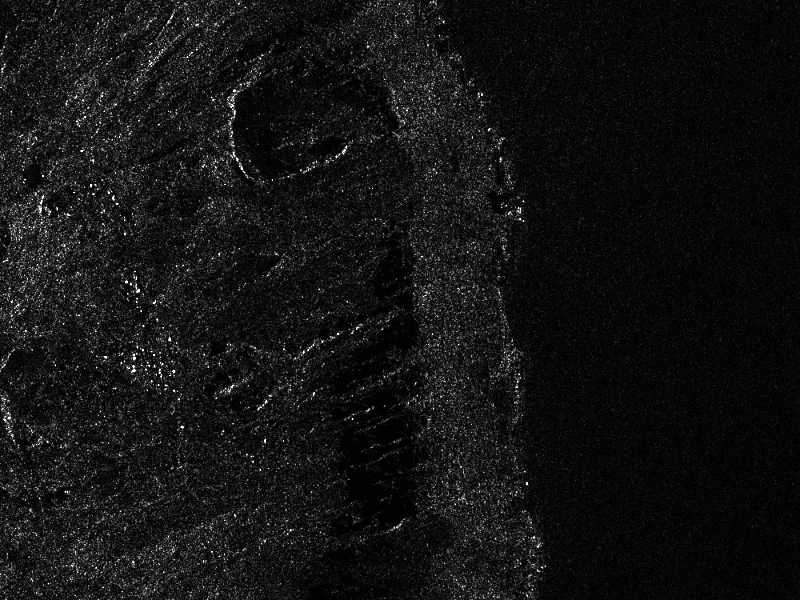
\includegraphics[width=0.45\textwidth]{../Art/S1-VV-extract-int.png}
  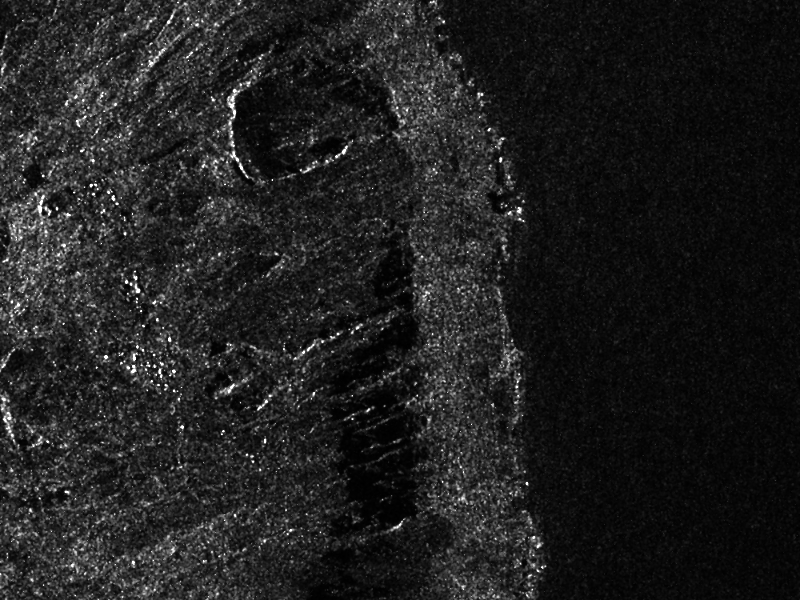
\includegraphics[width=0.45\textwidth]{../Art/S1-VV-despeckled-extract.png}
  \itkcaption[ExampleEpipolar]{Intensity image from a SLC-VV Sentinel1 image and
  result of Gamma filter.}
  \label{fig:S1VVdespeckledextract}
\end{figure}

\subsection{Polarimetry}

In conventional imaging radar the measurement is a scalar which is proportional
to the received back-scattered power at a particular combination of linear
polarization (HH, HV, VH or VV). 
Polarimetry is the measurement and interpretation of the polarization of this
measurement which allows to measure various optical properties of a material.
In polarimetry the basic measurement is a $2x2$ complex scattering matrix
yielding an eight dimensional measurement space (Sinclair matrix). For
reciprocal targets where $HV=VH$, this space is compressed to five dimensions:
three amplitudes ($|HH|$, $|HV|$, and $|VV|$); and two phase measurements,
(co-pol: HH-VV, and cross-pol:
HH-HV). (see \href{http://www.grss-ieee.org/technical-briefs/imaging-radar-polarimetry}{grss-ieee}).

\subsubsection{Matrix conversions}

This applications allows converting classical polarimetric matrices to each
other.  For instance, it is possible to get the coherency matrix from the
Sinclair one, or the Mueller matrix from the coherency one.  The figure below
(\ref{fig:polconv}) shows the workflow used in this application.

\begin{figure}[!h]
  \centering
   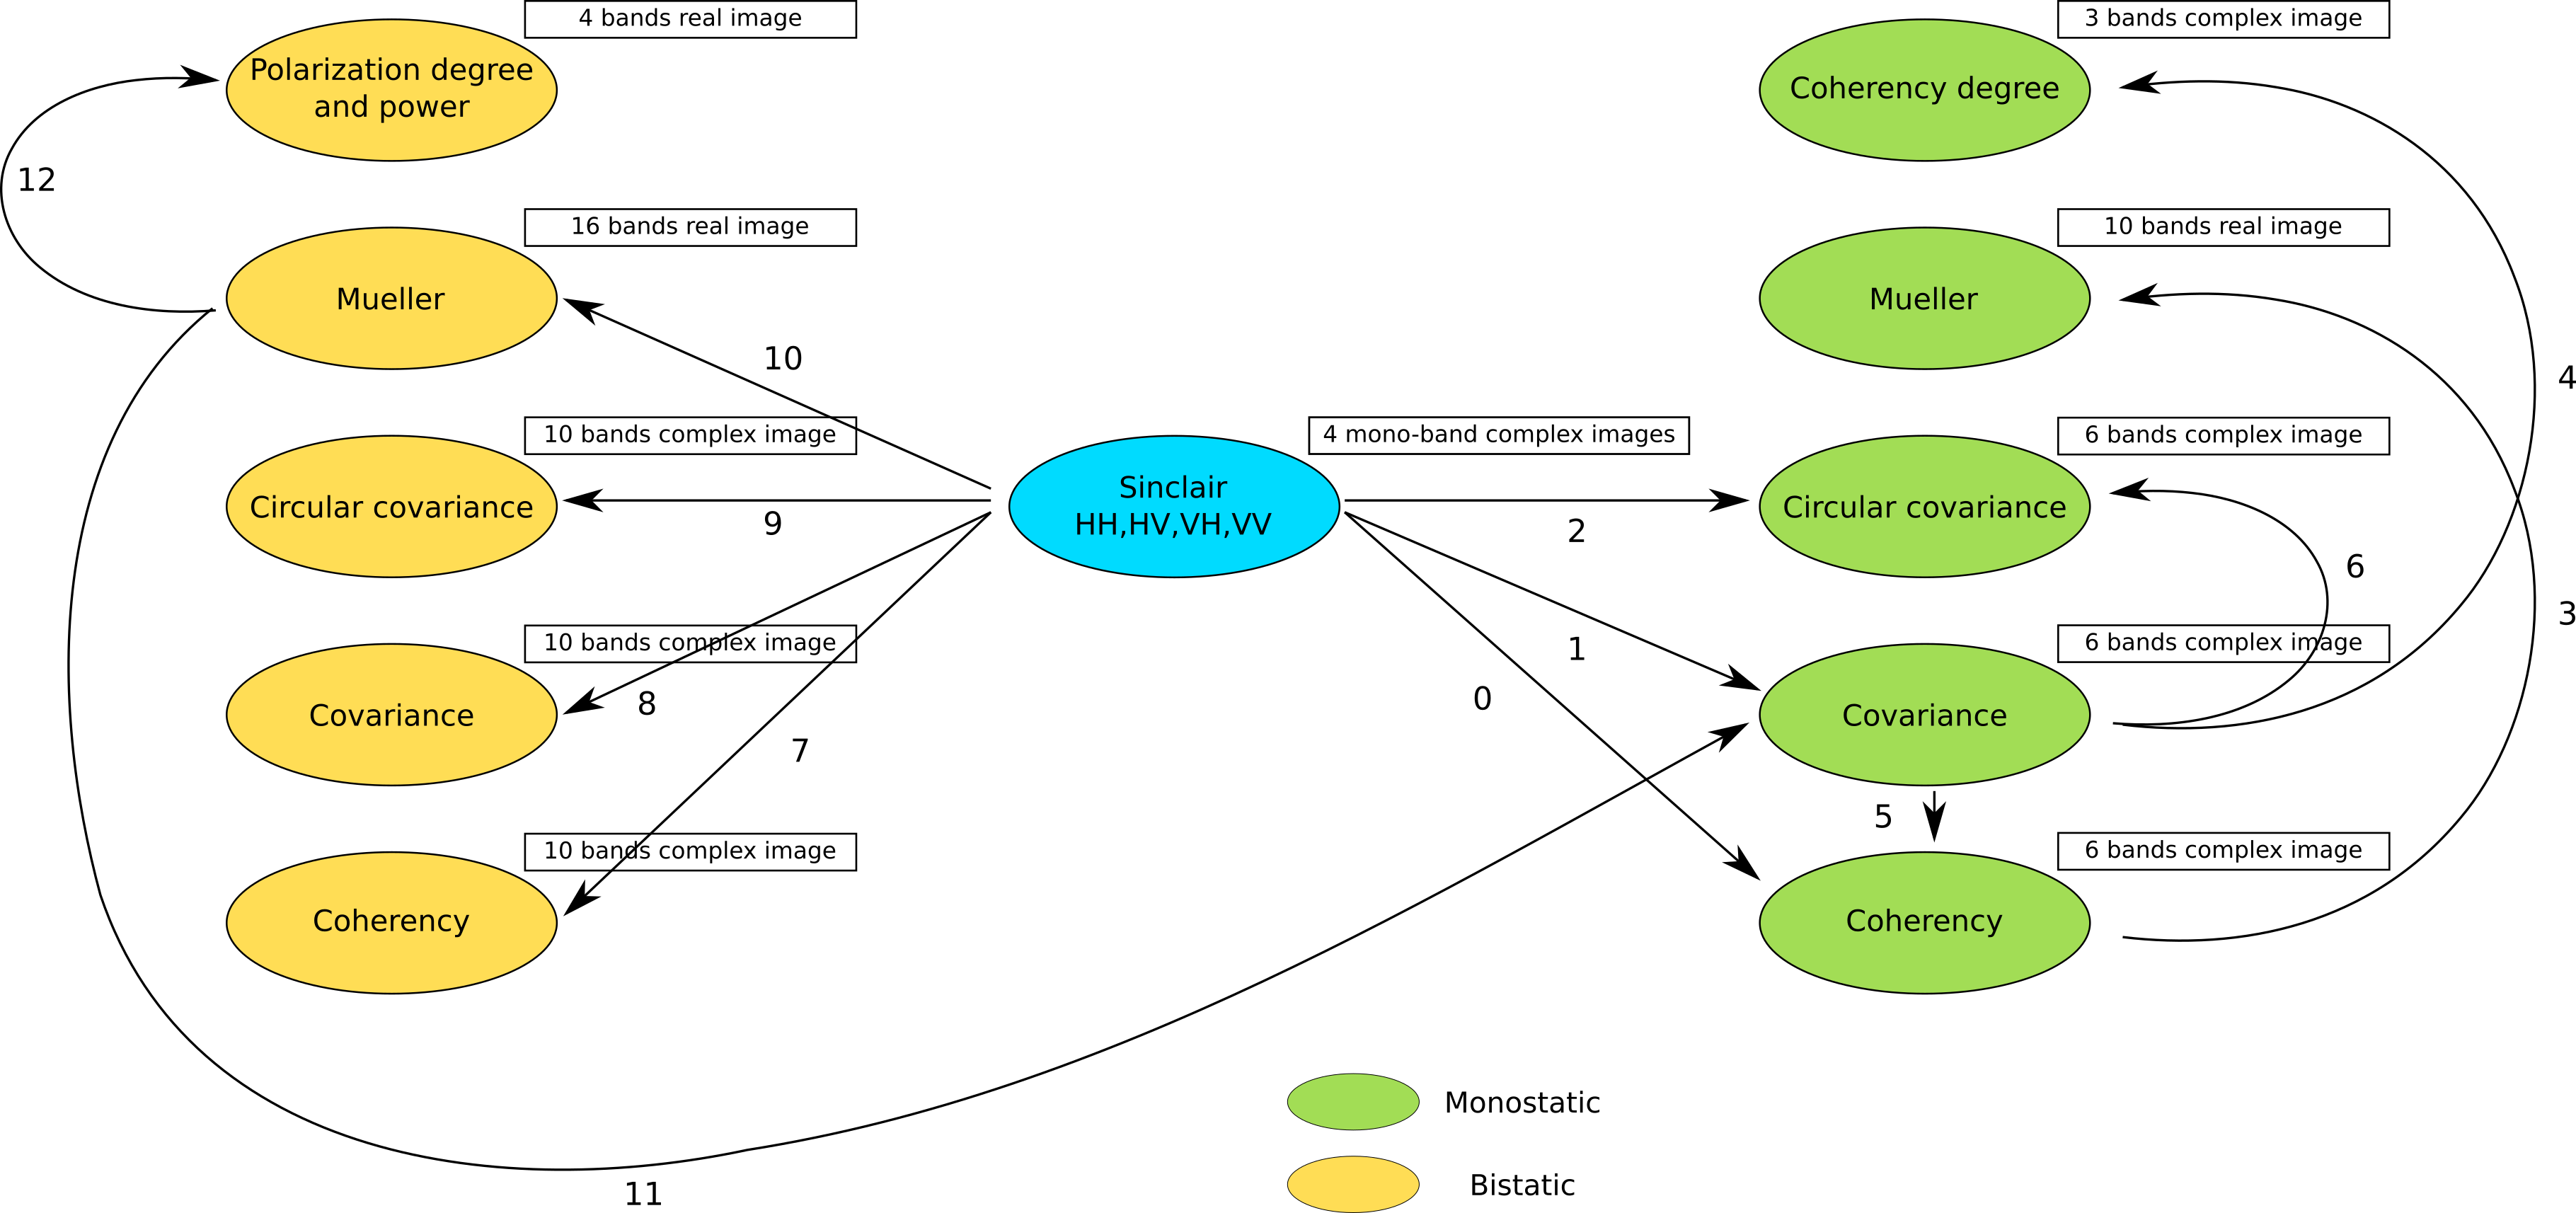
\includegraphics[width=\textwidth]{../Art/sarpol_conversion_schema.png}
  \itkcaption[SAR polarimetry conversion]{SAR polarimetry conversion application.}
  \label{fig:polconv}
\end{figure}

The filters used in this application never handle matrices, but images where
each band is related to their elements.  As most of the time SAR polarimetry
handles symmetric matrices, only the relevant elements are stored, so that the
images representing them have a minimal number of bands.  For instance, the
coherency matrix size is 3x3 in the monostatic case, and 4x4 in the bistatic
case : it will thus be stored in a 6-band or a 10-band complex image (the
diagonal and the upper elements of the matrix).

The Sinclair matrix is a special case : it is always represented as 3 or 4
one-band complex images (for mono- or bistatic case).

There are 13 available conversions, each one being related to the following  parameters:
\begin{enumerate}
\item msinclairtocoherency
\item msinclairtocovariance
\item msinclairtocircovariance
\item mcoherencytomueller
\item mcovariancetocoherencydegree
\item mcovariancetocoherency
\item mlinearcovariancetocircularcovariance
\item muellertomcovariance
\item bsinclairtocoherency
\item bsinclairtocovariance
\item bsinclairtocircovariance
\item sinclairtomueller
\item muellertopoldegandpower
\end{enumerate}

For each option parameter, the list below gives the formula used.

--- Monostatic case ---

\begin{enumerate}
\renewcommand{\labelenumii}{Channel \arabic{enumii} : }
\item msinclairtocoherency (SinclairToReciprocalCoherencyMatrixFunctor)
\begin{enumerate}
\item $ 0.5 . (S_{hh}+S_{vv}).(S_{hh}+S_{vv})^{*} $
\item $ 0.5 . (S_{hh}+S_{vv}).(S_{hh}-S_{vv})^{*} $
\item $ 0.5 . (S_{hh}+S_{vv}).(2 S_{hv})^{*} $
\item $ 0.5 . (S_{hh}-S_{vv}).(S_{hh}-S_{vv})^{*} $
\item $ 0.5 . (S_{hh}-S_{vv}).(2 S_{hv})^{*} $
\item $ 0.5 . (2 S_{hv}).(2 S_{hv})^{*} $
\end{enumerate}
 
\item msinclairtocovariance (SinclairToReciprocalCovarianceMatrixFunctor)
\begin{enumerate}
\item $ S_{hh}.S_{hh}^{*} $ 
\item $ \sqrt{2}.S_{hh}.S_{hv}^{*} $ 
\item $ S_{hh}.S_{vv}^{*} $ 
\item $ 2.S_{hv}.S_{hv}^{*} $ 
\item $ \sqrt{2}.S_{hv}.S_{vv}^{*} $ 
\item $ S_{vv}.S_{vv}^{*} $
\end{enumerate}
 
\item msinclairtocircovariance (SinclairToReciprocalCircularCovarianceMatrixFunctor)
\begin{enumerate}
\item $ S_{ll}.S_{ll}^{*} $ 
\item $ S_{ll}.S_{lr}^{*} $ 
\item $ S_{ll}.S_{rr}^{*} $ 
\item $ S_{lr}.S_{lr}^{*} $ 
\item $ S_{lr}.S_{rr}^{*} $ 
\item $ S_{rr}.S_{rr}^{*} $
\end{enumerate}

With:
\begin{itemize} 
\item $ S_{ll} = 0.5(S_{hh}+2j S_{hv}-S_{vv}) $ 
\item $ S_{lr} = 0.5(j S_{hh}+j S_{vv}) $  
\item $ S_{rr} = 0.5(-S_{hh}+2j S_{hv}+S_{vv}) $ 
\end{itemize}
 
\item mcoherencytomueller (ReciprocalCoherencyToReciprocalMuellerFunctor)
\begin{enumerate}
\item $ 0.5*( C_{11}+C_{22}+C_{33} ) $ 
\item $ Re(C_{12}) + Im(C_{22}) $ 
\item $ Re(C_{13}) $ 
\item $ Im(C_{23}) $ 
\item $ Re(C_{12}) $ 
\item $ 0.5*( C_{11}+C_{22}-C_{33} ) $ 
\item $ Re(C_{23}) $ 
\item $ Im(C_{13}) $ 
\item $ -Re(C_{13}) $ 
\item $ -Re(C_{23}) $
\item $ 0.5.Re(VAL1) $
\item $ 0.5.Im(VAL0) $
\item $ Im(C_{23}) $
\item $ Im(C_{13}) $
\item $ 0.5.Im(VAL1^{*}) $
\item $ 0.5.Re(VAL0) $
\end{enumerate}

With:
\begin{itemize} 
\item $ VAL0 = C_{33}+C_{12}-C_{11}-(C_{12}-C_{22})^{*}  $ 
\item $ VAL1 = -C_{33}+C_{12}-C_{11}-(C_{12}-C_{22})^{*} $ 
\end{itemize}

Where $C_{ij}$ are related to the elements of the reciprocal coherence matrix.
 
 
\item mcovariancetocoherencydegree (ReciprocalCovarianceToCoherencyDegreeFunctor)
\begin{enumerate}
\item $ abs(S_{hh}.S_{vv}^{*}) / sqrt(S_{hh}.S_{hh}^{*}) / sqrt(S_{vv}.S_{vv}^{*}) $ 
\item $ abs(S_{hv}.S_{vv}^{*}) / sqrt(S_{hv}.S_{hv}^{*}) / sqrt(S_{vv}.S_{vv}^{*}) $ 
\item $ abs(S_{hh}.S_{hv}^{*}) / sqrt(S_{hh}.S_{hh}^{*}) / sqrt(S_{hv}.S_{hv}^{*}) $
\end{enumerate}
 
\item mcovariancetocoherency (ReciprocalCovarianceToReciprocalCoherencyFunctor)
\begin{enumerate}
\item $ 0.5 . ( C_{33} + C_{13} + C_{13}^{*} + C_{11} ) $ 
\item $ 0.5 . ( -C_{33} - C_{13} + C_{13}^{*} + C_{11} ) $ 
\item $ 0.5 . ( \sqrt{2}.C_{12} + \sqrt{2}.C_{23}^{*} ) $ 
\item $ 0.5 . ( C_{33} - C_{13} - C_{13}^{*} + C_{11} ) $ 
\item $ 0.5 . ( \sqrt{2}.C_{12} - \sqrt{2}.C_{23}^{*} ) $ 
\item $ 0.5 . ( 2 . C_{22} ) $
\end{enumerate}

Where $C_{ij}$ are related to the elements of the reciprocal linear covariance
matrix.
 
\item mlinearcovariancetocircularcovariance (ReciprocalLinearCovarianceToReciprocalCircularCovarianceFunctor)
\begin{enumerate}
\item $ 0.25 . ( C_{33}-i.\sqrt{2}.C_{23}-C_{13}+i.\sqrt{2}.C_{23}^{*}-C_{13}^{*}+2.C_{22}-i.\sqrt{2}.C_{12}+i.\sqrt{2}.C_{12}^{*}+C_{11} ) $ 
\item $ 0.25 . ( i.\sqrt{2}.C_{33}+2.C_{23}-i.\sqrt{2}.C_{13}+i.\sqrt{2}.C_{13}^{*}+2.C_{12}^{*}-i.\sqrt{2}.C_{11} ) $ 
\item $ 0.25 . ( -C_{33}+i.\sqrt{2}.C_{23}+C_{13}+i.\sqrt{2}.C_{23}^{*}+C_{13}^{*}+2.C_{22}-i.\sqrt{2}.C_{12}-i.\sqrt{2}.C_{12}^{*}-C_{11} ) $ 
\item $ 0.25 . ( 2.C_{33}+2.C_{13}+2.C_{13}^{*}+2.C_{11} ) $ 
\item $ 0.25 . ( i.\sqrt{2}.C_{33}+i.\sqrt{2}.C_{13}+2.C_{23}^{*}-i.\sqrt{2}.C_{13}^{*}+2.C_{12}-i.\sqrt{2}.C_{11} ) $ 
\item $ 0.25 . ( C_{33}+i.\sqrt{2}.C_{23}-C_{13}-i.\sqrt{2}.C_{23}^{*}-C_{13}^{*}+2.C_{22}+i.\sqrt{2}.C_{12}-i.\sqrt{2}.C_{12}^{*}+C_{11} ) $
\end{enumerate}

Where $C_{ij}$ are related to the elements of the reciprocal linear covariance
matrix.

\item muellertomcovariance (MuellerToReciprocalCovarianceFunctor)
\begin{enumerate}
\item $ 0.5.(M_{11}+M_{22}+2.M_{12}) $ 
\item $ 0.5.\sqrt{2}.[(M_{13}+M_{23}) + j.(M_{14}+M_{24})] $ 
\item $ -0.5.(M_{33}+M_{44}) - j.M_{34} $ 
\item $ M_{11}-M_{22} $ 
\item $ 0.5.\sqrt{2}.[(M_{13}-M_{23}) + j.(M_{14}-M_{24})] $ 
\item $ 0.5.(M_{11}+M_{22}-2.M_{12}) $
\end{enumerate}

\end{enumerate}

--- Bistatic case ---

\begin{enumerate}
\renewcommand{\labelenumii}{Channel \arabic{enumii} : }
\setcounter{enumi}{8}

\item bsinclairtocoherency (SinclairToCoherencyMatrixFunctor)
\begin{enumerate}
\item $ (S_{hh}+S_{vv}).(S_{hh}+S_{vv})^{*} $ 
\item $ (S_{hh}+S_{vv}).(S_{hh}-S_{vv})^{*} $ 
\item $ (S_{hh}+S_{vv}).(S_{hv}+S_{vh})^{*} $ 
\item $ (S_{hh}+S_{vv}).( j (S_{hv}-S_{vh}))^{*} $ 
\item $ (S_{hh}-S_{vv}).(S_{hh}-S_{vv})^{*} $ 
\item $ (S_{hh}-S_{vv}).(S_{hv}+S_{vh})^{*} $ 
\item $ (S_{hh}-S_{vv}).( j (S_{hv}-S_{vh}))^{*} $ 
\item $ (S_{hv}+S_{vh}).(S_{hv}+S_{vh})^{*} $ 
\item $ (S_{hv}+S_{vh}).( j (S_{hv}-S_{vh}))^{*} $ 
\item $ j (S_{hv}-S_{vh}).( j (S_{hv}-S_{vh}))^{*} $
\end{enumerate}
 
\item bsinclairtocovariance (SinclairToCovarianceMatrixFunctor)
\begin{enumerate}
\item $ S_{hh}.S_{hh}^{*} $ 
\item $ S_{hh}.S_{hv}^{*} $ 
\item $ S_{hh}.S_{vh}^{*} $ 
\item $ S_{hh}.S_{vv}^{*} $ 
\item $ S_{hv}.S_{hv}^{*} $ 
\item $ S_{hv}.S_{vh}^{*} $ 
\item $ S_{hv}.S_{vv}^{*} $ 
\item $ S_{vh}.S_{vh}^{*} $ 
\item $ S_{vh}.S_{vv}^{*} $ 
\item $ S_{vv}.S_{vv}^{*} $
\end{enumerate}
 
\item bsinclairtocircovariance (SinclairToCircularCovarianceMatrixFunctor)
\begin{enumerate}
\item $ S_{ll}.S_{ll}^{*} $ 
\item $ S_{ll}.S_{lr}^{*} $ 
\item $ S_{ll}.S_{rl}^{*} $ 
\item $ S_{ll}.S_{rr}^{*} $ 
\item $ S_{lr}.S_{lr}^{*} $ 
\item $ S_{lr}.S_{rl}^{*} $ 
\item $ S_{lr}.S_{rr}^{*} $ 
\item $ S_{rl}.S_{rl}^{*} $ 
\item $ S_{rl}.S_{rr}^{*} $ 
\item $ S_{rr}.S_{rr}^{*} $ 
\end{enumerate}

With:
\begin{itemize} 
\item $ S_{ll} = 0.5(S_{hh}+j S_{hv}+j S_{vh}-S_{vv}) $ 
\item $ S_{lr} = 0.5(j S_{hh}+S_{hv}-S_{vh}+j S_{vv}) $ 
\item $ S_{rl} = 0.5(j S_{hh}-S_{hv}+ S_{vh}+j S_{vv}) $ 
\item $ S_{rr} = 0.5(-S_{hh}+j S_{hv}+j S_{vh}+S_{vv}) $ 
\end{itemize}

--- Both cases ---

\item sinclairtomueller (SinclairToMueller)
\begin{enumerate} 
\item $ 0.5 Re( T_{xx}.T_{xx}^{*} + T_{xy}.T_{xy}^{*} + T_{yx}.T_{yx}^{*} + T_{yy}.T_{yy}^{*} ) $ 
\item $ 0.5 Re( T_{xx}.T_{xx}^{*} - T_{xy}.T_{xy}^{*} + T_{yx}.T_{yx}^{*} - T_{yy}.T_{yy}^{*} ) $ 
\item $ Re( T_{xx}.T_{xy}^{*} + T_{yx}.T_{yy}^{*} ) $ 
\item $ Im( T_{xx}.T_{xy}^{*} + T_{yx}.T_{yy}^{*} ) $ 
\item $ 0.5 Re( T_{xx}.T_{xx}^{*} + T_{xy}.T_{xy}^{*} - T_{yx}.T_{yx}^{*} - T_{yy}.T_{yy}^{*} ) $ 
\item $ 0.5 Re( T_{xx}.T_{xx}^{*} - T_{xy}.T_{xy}^{*} - T_{yx}.T_{yx}^{*} + T_{yy}.T_{yy}^{*} ) $ 
\item $ Re( T_{xx}.T_{xy}^{*} - T_{yx}.T_{yy}^{*} ) $ 
\item $ Im( T_{xx}.T_{xy}^{*} - T_{yx}.T_{yy}^{*} ) $ 
\item $ Re( T_{xx}.T_{yx}^{*} + T_{xy}.T_{yy}^{*} ) $ 
\item $ Im( T_{xx}.T_{yx}^{*} - T_{xy}.T_{yy}^{*} ) $ 
\item $ Re( T_{xx}.T_{yy}^{*} + T_{xy}.T_{yx}^{*} ) $ 
\item $ Im( T_{xx}.T_{yy}^{*} - T_{xy}.T_{yx}^{*} ) $ 
\item $ Re( T_{xx}.T_{yx}^{*} + T_{xy}.T_{yy}^{*} ) $ 
\item $ Im( T_{xx}.T_{yx}^{*} - T_{xy}.T_{yy}^{*} ) $ 
\item $ Re( T_{xx}.T_{yy}^{*} + T_{xy}.T_{yx}^{*} ) $ 
\item $ Im( T_{xx}.T_{yy}^{*} - T_{xy}.T_{yx}^{*} ) $
\end{enumerate}

With :
\begin{itemize}
\item $ T_{xx} = -S_{hh} $ 
\item $ T_{xy} = -S_{hv} $ 
\item $ T_{yx} = S_{vh} $ 
\item $ T_{yy} = S_{vv} $ 
\end{itemize}
 
\item muellertopoldegandpower (MuellerToPolarisationDegreeAndPowerFunctor)
\begin{enumerate}
\item $ P_{min} $ 
\item $ P_{max} $ 
\item $ DegP_{min} $ 
\item $ DegP_{max} $
\end{enumerate}

\end{enumerate}

Examples :

\begin{enumerate}
\item 
\begin{verbatim} 
otbcli_SARPolarMatrixConvert -inhh imageryC_HH.tif 
                             -inhv imageryC_HV.tif 
                             -invv imageryC_VV.tif
                             -conv msinclairtocoherency
                             -outc coherency.tif 
\end{verbatim}
									  
\item 
\begin{verbatim} 
otbcli_SARPolarMatrixConvert -inhh imageryC_HH.tif 
                             -inhv imageryC_HV.tif 
                             -invv imageryC_VV.tif
		             -conv msinclairtocovariance
                             -outc covariance.tif 
\end{verbatim}
									  
\item 
\begin{verbatim} 
otbcli_SARPolarMatrixConvert -inhh imageryC_HH.tif 
                             -inhv imageryC_HV.tif 
                             -invv imageryC_VV.tif
	                     -conv msinclairtocircovariance
                             -outc circ_covariance.tif 
\end{verbatim}
									  
\item 
\begin{verbatim} 
otbcli_SARPolarMatrixConvert -inc coherency.tif 
		             -conv mcoherencytomueller
                             -outf mueller.tif 
\end{verbatim}
									  
\item 
\begin{verbatim} 
otbcli_SARPolarMatrixConvert -inc covariance.tif 
		             -conv mcovariancetocoherencydegree
                             -outc coherency_degree.tif 
\end{verbatim}
									  
\item 
\begin{verbatim} 
otbcli_SARPolarMatrixConvert -inc covariance.tif 
			     -conv mcovariancetocoherency
                             -outc coherency.tif 
\end{verbatim}
									  
\item 
\begin{verbatim} 
otbcli_SARPolarMatrixConvert -inc covariance.tif 
			     -conv mlinearcovariancetocircularcovariance
                             -outc circ_covariance.tif 
\end{verbatim}	
									  			
\item 
\begin{verbatim} 
otbcli_SARPolarMatrixConvert -inf mueller.tif 
			     -conv muellertomcovariance
                             -outc covariance.tif 
\end{verbatim}	
									  								  
\item 
\begin{verbatim} 
otbcli_SARPolarMatrixConvert -inhh imageryC_HH.tif 
                             -inhv imageryC_HV.tif 
                             -invh imageryC_VH.tif 
                             -invv imageryC_VV.tif
			     -conv bsinclairtocoherency
                             -outc bcoherency.tif 
\end{verbatim}
									  
\item 
\begin{verbatim} 
otbcli_SARPolarMatrixConvert -inhh imageryC_HH.tif 
                             -inhv imageryC_HV.tif 
                             -invh imageryC_VH.tif 
                             -invv imageryC_VV.tif 
			     -conv bsinclairtocovariance
                             -outc bcovariance.tif 
\end{verbatim}
									  
\item 
\begin{verbatim} 
otbcli_SARPolarMatrixConvert -inhh imageryC_HH.tif 
                             -inhv imageryC_HV.tif 
                             -invh imageryC_VH.tif 
                             -invv imageryC_VV.tif
		             -conv bsinclairtocircovariance
                             -outc circ_bcovariance.tif 
\end{verbatim}
									  
									  
\item 
\begin{verbatim} 
otbcli_SARPolarMatrixConvert -inhh imageryC_HH.tif 
                             -inhv imageryC_HV.tif 
                             -invh imageryC_VH.tif 
                             -invv imageryC_VV.tif 
			     -conv sinclairtomueller
                             -outf mueller.tif 
\end{verbatim}
									  
\item 
\begin{verbatim} 
otbcli_SARPolarMatrixConvert -inf mueller.tif 
		             -conv muellertopoldegandpower
                             -outf degreepower.tif 
\end{verbatim}
									  
\end{enumerate}

\subsubsection{Polarimetric decompositions}

From one-band complex images (HH, HV, VH, VV), returns the selected
decomposition.  The H-alpha-A decomposition is currently the only one available;
it is implemented for the monostatic case (transmitter and receiver are
co-located).  User must provide three one-band complex images HH, HV or VH, and
VV (HV = VH in monostatic case).  The H-alpha-A decomposition consists in
averaging 3x3 complex coherency matrices (incoherent analysis) : The user must
provide the size of the averaging window, thanks to the parameter
inco.kernelsize.  The applications returns a float vector image, made of three
channels : H(entropy), Alpha, A(Anisotropy).

Here are the formula used (refer to the previous section about how the coherence
matrix is obtained from the Sinclair one):
\begin{enumerate}
\renewcommand{\labelenumii}{Channel \arabic{enumii} : }
\item $ entropy = -\sum_{i=0}^{2} \frac{p[i].\log{p[i]}}{\log{3}} $
\item $ \alpha = \sum_{i=0}^{2} p[i].\alpha_{i} $
\item $ anisotropy = \frac {SortedEigenValues[1] - SortedEigenValues[2]}{SortedEigenValues[1] + SortedEigenValues[2]} $
\end{enumerate}

Where:
\begin{itemize}
\item $ p[i] = max(SortedEigenValues[i], 0) / \sum_{i=0}^{2, SortedEigenValues[i]>0} SortedEigenValues[i] $
\item $ \alpha_{i} = \left| SortedEigenVector[i] \right|* \frac{180}{\pi}$
\end{itemize}


Example :

We first extract a ROI from the original image (not required). 
Here imagery\_HH.tif represents the element HH of the Sinclair matrix (and so forth).

\begin{itemize}
\item 
\begin{verbatim} 
otbcli_ExtractROI -in imagery_HH.tif -out imagery_HH_extract.tif  
		  -startx 0 -starty 0 
                  -sizex 1000 -sizey 1000 
\end{verbatim}
									  
\item 
\begin{verbatim} 
otbcli_ExtractROI -in imagery_HV.tif -out imagery_HV_extract.tif  
		  -startx 0 -starty 0
                  -sizex 1000 -sizey 1000 
\end{verbatim}
									  
\item 
\begin{verbatim} 
otbcli_ExtractROI -in imagery_VV.tif -out imagery_VV_extract.tif  
		  -startx 0 -starty 0
                  -sizex 1000 -sizey 1000 
\end{verbatim}
\end{itemize}

Next we apply the H-alpha-A decomposition:

\begin{verbatim} 
otbcli_SARDecompositions -inhh imagery_HH_extract.tif 
                         -inhv imagery_HV_extract.tif 
                         -invv imagery_VV_extract.tif 
			 -decomp haa -inco.kernelsize 5 
                         -out haa_extract.tif 
\end{verbatim}

The result has three bands : entropy (0..1) - alpha (0..90) - anisotropy
(0..1). It is splitted into 3 mono-band images thanks to following command :

\begin{verbatim} 
otbcli_SplitImage -in haa_extract.tif -out haa_extract_splitted.tif 
\end{verbatim}

Each image is then colored thanks to a color look-up table 'hot'. 
Notice how minimum and maximum values are provided for each polarimetric variable.

\begin{itemize}
\item 
\begin{verbatim} 
otbcli_ColorMapping -in haa_extract_splitted_0.tif 
                    -method continuous -method.continuous.lut hot 
                    -method.continuous.min 0 
                    -method.continuous.max 1
                    -out entropy_hot.tif uint8 
\end{verbatim}
									  
\item 
\begin{verbatim} 
otbcli_ColorMapping -in haa_extract_splitted_1.tif -method continuous 
    -method.continuous.lut hot -method.continuous.min 0 -method.continuous.max
    90 -out alpha_hot.tif uint8 
\end{verbatim}
									  
\item 
\begin{verbatim} 
otbcli_ColorMapping -in haa_extract_splitted_2.tif 
                    -method continuous -method.continuous.lut hot 
                    -method.continuous.min 0 
                    -method.continuous.max 1
                    -out anisotropy_hot.tif uint8 
\end{verbatim}
\end{itemize}

The results are shown in the figures below (\ref{fig:entropyimage}
, \ref{fig:alphaimage} and \ref{fig:anisotropyimage}).
\begin{figure}[!h]
\center
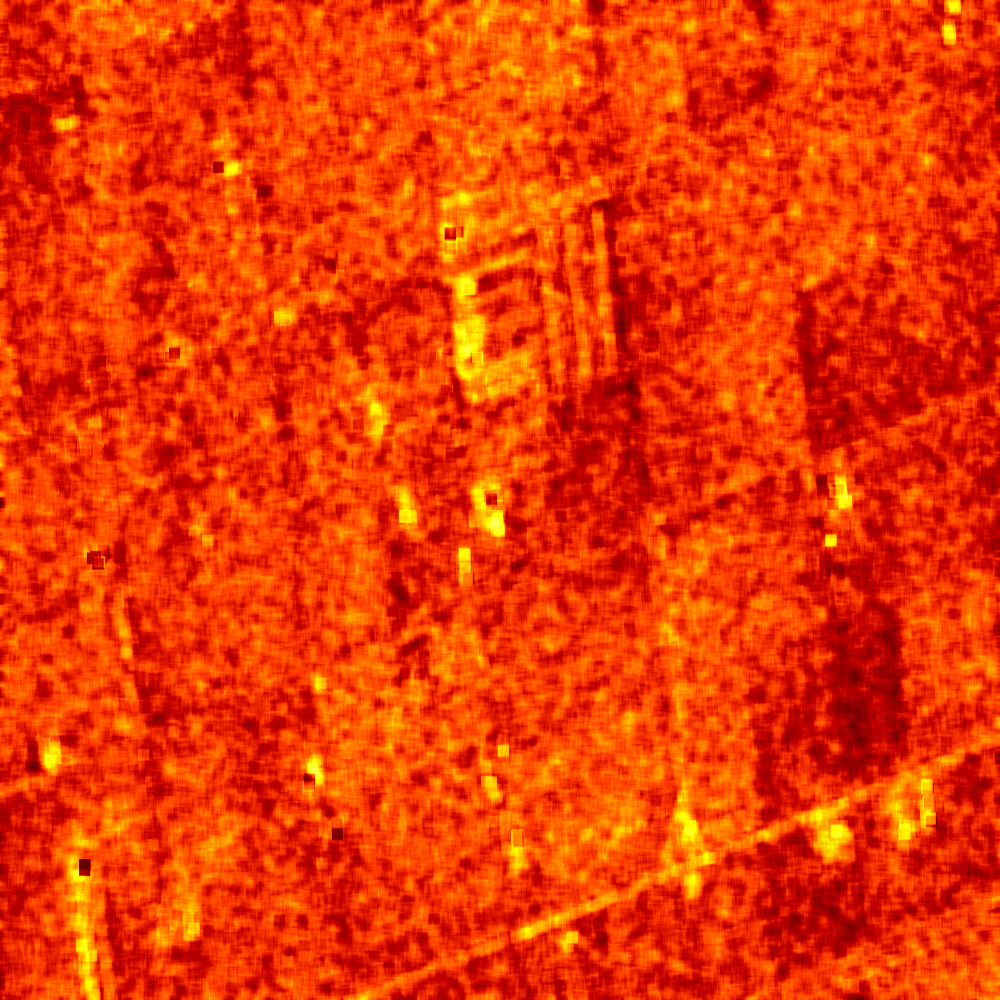
\includegraphics[width=0.7\textwidth]{../Art/entropyhot.png}
\itkcaption[SAR decomp]{Entropy image.}
\label{fig:entropyimage}
\end{figure}

\begin{figure}[!h]
\center
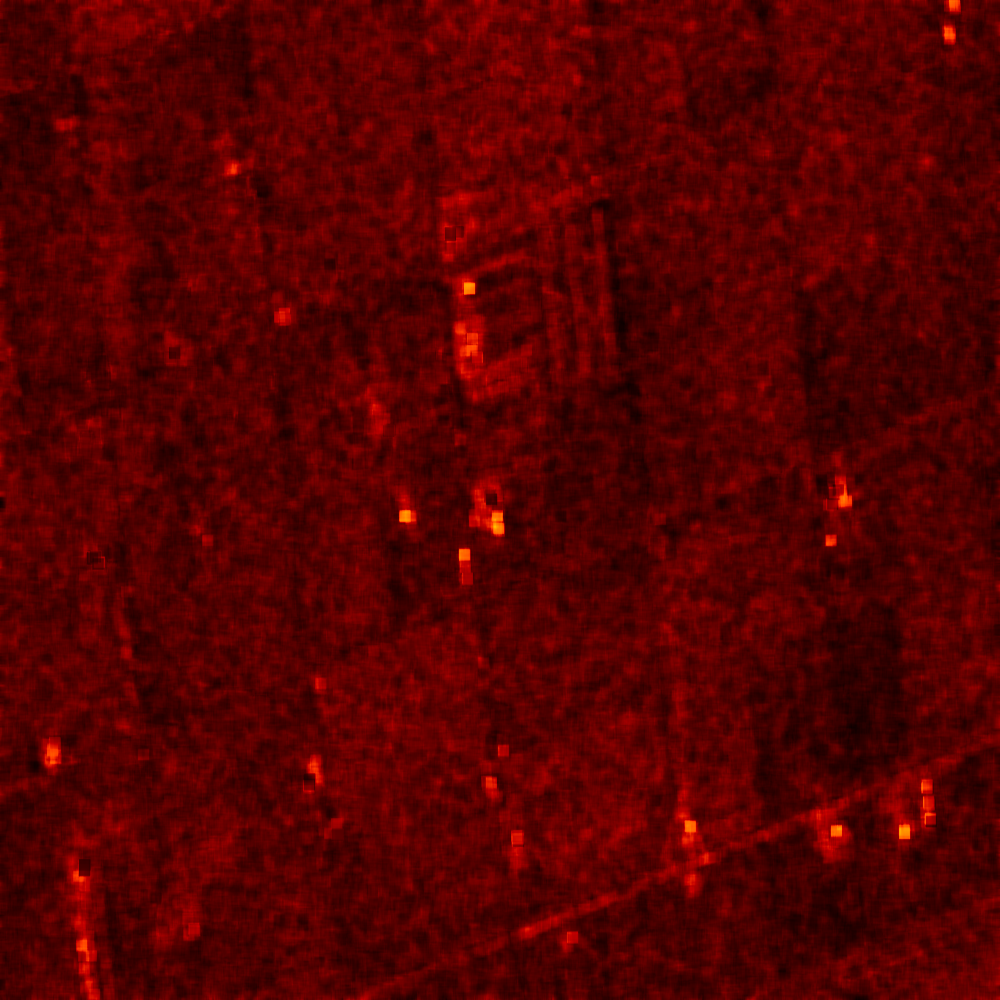
\includegraphics[width=0.7\textwidth]{../Art/alphahot.png}
\itkcaption[SAR decomp]{Alpha image.}
\label{fig:alphaimage}
\end{figure}

\begin{figure}[!h]
\center
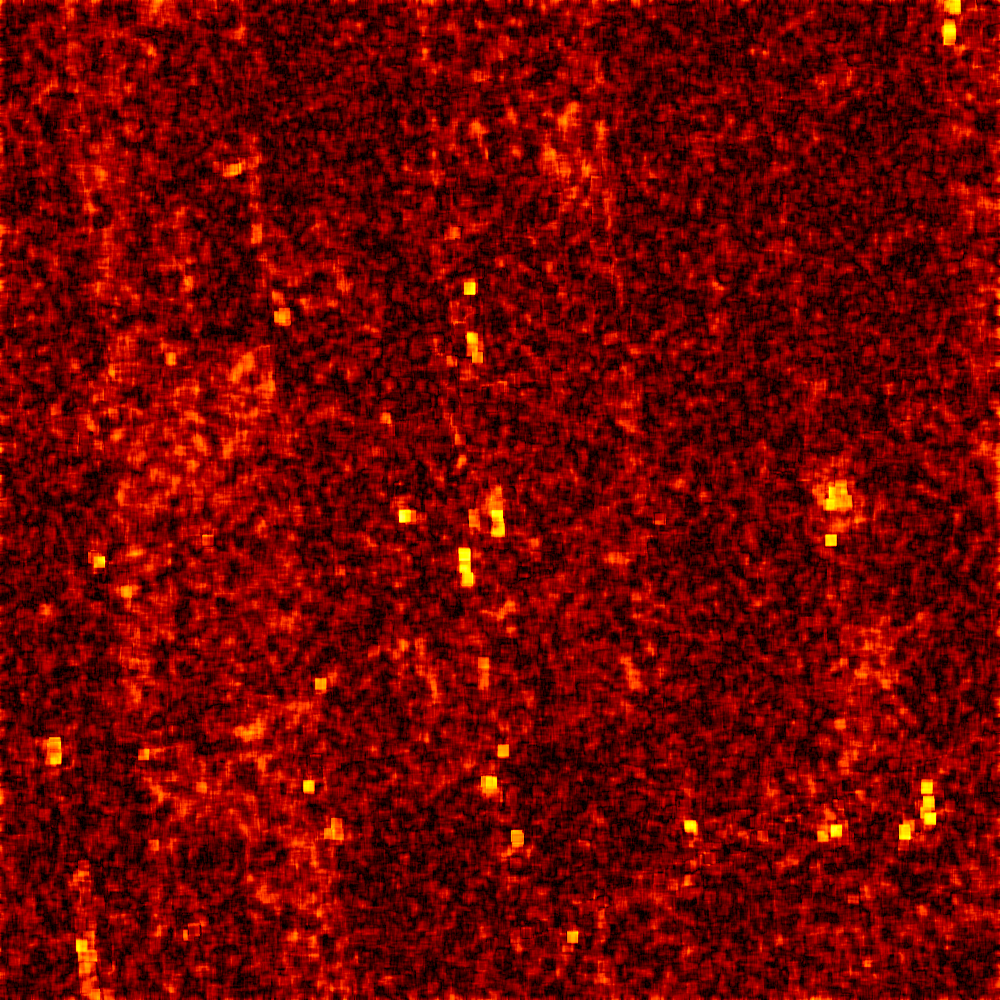
\includegraphics[width=0.7\textwidth]{../Art/anisotropyhot.png}
\itkcaption[SAR decomp]{Anisotropy image.}
\label{fig:anisotropyimage}
\end{figure}

\subsubsection{Polarimetric synthetis}

This application gives, for each pixel, the power that would have been received
by a SAR system with a basis different from the classical (H,V) one
(polarimetric synthetis).  The new basis are indicated through two Jones
vectors, defined by the user thanks to orientation (psi) and ellipticity (khi)
parameters.  These parameters are namely psii, khii, psir and khir. The suffixes
(i) and (r) refer to the transmitting antenna and the receiving antenna
respectively.  Orientations and ellipticity are given in degrees, and are
between -90/90 degrees and -45/45 degrees respectively.

Four polarization architectures can be processed :
\begin{enumerate}
\item HH\_HV\_VH\_VV : full polarization, general bistatic case.
\item HH\_HV\_VV or HH\_VH\_VV : full polarization, monostatic case (transmitter
and receiver are co-located).
\item HH\_HV : dual polarization.
\item VH\_VV : dual polarization.
\end{enumerate}
The application takes a complex vector image as input, where each band
correspond to a particular emission/reception polarization scheme.  User must
comply with the band order given above, since the bands are used to build the
Sinclair matrix.

In order to determine the architecture, the application first relies on the
number of bands of the input image.
\begin{enumerate}
\item Architecture HH\_HV\_VH\_VV is the only one with four bands, there is no
possible confusion.
\item Concerning HH\_HV\_VV and HH\_VH\_VV architectures, both correspond to a
three channels image. But they are processed in the same way, as the Sinclair
matrix is symmetric in the monostatic case.
\item Finally, the two last architectures (dual-polarization), can't be
distinguished only by the number of bands of the input image. User must then use
the parameters emissionh and emissionv to indicate the architecture of the
system : emissionh=1 and emissionv=0 for HH\_HV, emissionh=0 and emissionv=1 for
VH\_VV.
\end{enumerate}
Note : if the architecture is HH\_HV, khii and psii are automatically set to 0/0
degrees; if the architecture is VH\_VV, khii and psii are automatically set to
0/90 degrees.

It is also possible to force the calculation to co-polar or cross-polar modes.
In the co-polar case, values for psir and khir will be ignored and forced to
psii and khii; same as the cross-polar mode, where khir and psir will be forced
to psii + 90 degrees and -khii.

Finally, the result of the polarimetric synthesis is expressed in the power
domain, through a one-band scalar image.
 
The final formula is thus : $P=\mid B^T.[S].A\mid^2$ , where A ans B are two
Jones vectors and S is a Sinclair matrix.
 
The two figures below (\ref{fig:polsynthll} and \ref{fig:polsynthlr}) show the
two images obtained with the basis LL and LR (L for left circular polarization
and R for right polarization), from a Radarsat-2 image taken over
Vancouver, Canada. Once the four two-band images imagery\_HH imagery\_HV imagery\_VH
imagery\_VV were merged into a single four complex band image
imageryC\_HH\_HV\_VH\_VV.tif, the following commands were used to produce the LL
and LR images :

\begin{verbatim} 
otbcli_SARPolarSynth -in imageryC_HH_HV_VH_VV.tif 
		     -psii 0 -khii 45 -mode co 
                     -out test-LL.tif 
\end{verbatim}
\begin{verbatim} 
otbcli_SARPolarSynth -in imageryC_HH_HV_VH_VV.tif
                     -psii 0 -khii 45 -mode cross 
                     -out test-LR.tif 
\end{verbatim}

The produced images were then rescaled to intensities ranging from 0 to 255 in
order to be displayed.

\begin{figure}[!h]
\center
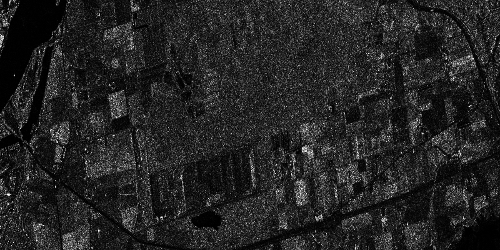
\includegraphics[width=0.7\textwidth]{../Art/test-left-co-2.png}
\itkcaption[SAR polarimetry conversion]{Image LL (sensor : RADARSAT-2).}
\label{fig:polsynthll}
\end{figure}

\begin{figure}[!h]
\center
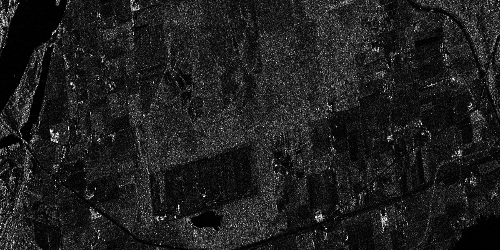
\includegraphics[width=0.7\textwidth]{../Art/test-left-cross-2.png}
\itkcaption[SAR polarimetry conversion]{Image LR (sensor : RADARSAT-2).}
\label{fig:polsynthlr}
\end{figure}

\subsubsection{Polarimetric data visualization}

Finally, let's talk about polarimetric data visualization. There is a strong
link between polarimetric data visualization and the way they can be decomposed
into significant physical processes.  Indeed, by setting the results (or
combinations) of such decompositions to RGB channels that help in interpreting
SAR polarimetric images.

There is no specific dedicated application yet, but it is possible to use a
combination of different applications as a replacement.  Let's do it with a
RADARSAT-2 acquisition over the famous place of the Golden Gate Bridge, San
Francisco, California.

We first make an extract from the original image (not mandatory). 

\begin{itemize}
\item 
\begin{verbatim} 
otbcli_ExtractROI -in imagery_HH.tif -out imagery_HH_extract.tif 
                  -startx 0 -starty 6300 
                  -sizex 2790 -sizey 2400 
\end{verbatim}
									  
\item 
\begin{verbatim} 
otbcli_ExtractROI -in imagery_HV.tif -out imagery_HV_extract.tif 
                  -startx 0 -starty 6300 
                  -sizex 2790 -sizey 2400 
\end{verbatim}
									  
\item 
\begin{verbatim} 
otbcli_ExtractROI -in imagery_VV.tif -out imagery_VV_extract.tif 
                  -startx 0 -starty 6300 
                  -sizex 2790 -sizey 2400 
\end{verbatim}
\end{itemize}

Then we compute the amplitude of each band using the \textbf{BandMath}
application:

\begin{itemize}
\item 
\begin{verbatim} 
otbcli_BandMath -il imagery_HH_extract.tif -out HH.tif 
                -exp "sqrt(im1b1^2+im1b2^2)" 
\end{verbatim}
									  
\item 
\begin{verbatim} 
otbcli_BandMath -il imagery_HV_extract.tif -out HV.tif
                -exp "sqrt(im1b1^2+im1b2^2)" 
\end{verbatim}
									  
\item 
\begin{verbatim} 
otbcli_BandMath -il imagery_VV_extract.tif -out VV.tif
                -exp "sqrt(im1b1^2+im1b2^2)" 
\end{verbatim}
\end{itemize}

Note that BandMath application interprets the image 'imagery\_XX\_extract.tif'
as an image made of two bands, where the first one is related to the real part
of the signal, and where the second one is related to the imaginary part (that's
why the modulus is obtained by the expressions $im1b1^2+im1b2^2$).

Then, we rescale the produced images to intensities ranging from 0 to 255:

\begin{itemize}
\item 
\begin{verbatim} 
otbcli_Rescale -in HH.tif -out HH_res.png uint8 
\end{verbatim}
									  
\item 
\begin{verbatim} 
otbcli_Rescale -in HV.tif -out HV_res.png uint8 
\end{verbatim}
									  
\item 
\begin{verbatim} 
otbcli_Rescale -in VV.tif -out VV_res.png uint8 
\end{verbatim}
\end{itemize}

Figures below (\ref{fig:hhfrisco} , \ref{fig:hvfrisco} and \ref{fig:vvfrisco}) show the images obtained :
\begin{figure}[!h]
\center
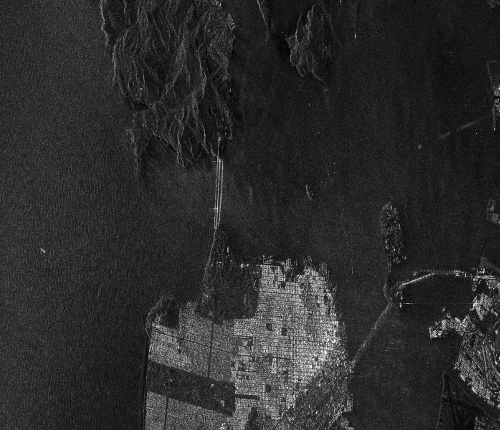
\includegraphics[width=0.7\textwidth]{../Art/RSAT2_HH_Frisco.png}
\itkcaption[SAR polarimetry visu]{Band HH in amplitude (sensor : RADARSAT2).}
\label{fig:hhfrisco}
\end{figure}

\begin{figure}[!h]
\center
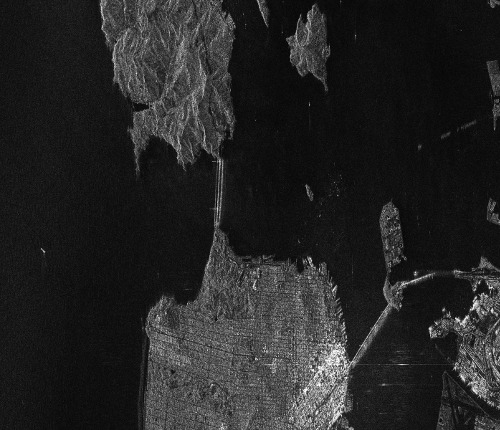
\includegraphics[width=0.7\textwidth]{../Art/RSAT2_HV_Frisco.png}
\itkcaption[SAR polarimetry visu]{Band HV in amplitude (sensor : RADARSAT2).}
\label{fig:hvfrisco}
\end{figure}

\begin{figure}[!h]
\center
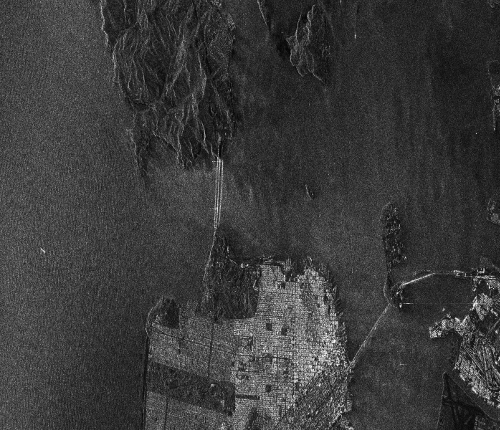
\includegraphics[width=0.7\textwidth]{../Art/RSAT2_VV_Frisco.png}
\itkcaption[SAR polarimetry visu]{Band VV in amplitude (sensor : RADARSAT2).}
\label{fig:vvfrisco}
\end{figure}

Now the most interesting step. In order to get a friendly coloration of these
data, we are going to use the Pauli decomposition, defined as follows :

\begin{itemize}
\item  $a=\frac{|S_{HH}-S_{VV}|}{\sqrt{2}}$ 
									  
\item  $b=\sqrt{2}.|S_{HV}|$ 
									  
\item  $c=\frac{|S_{HH}+S_{VV}|}{\sqrt{2}}$ 
\end{itemize}

We use the BandMath application again:

\begin{itemize}
\item 
\begin{verbatim} 
otbcli_BandMath -il imagery_HH_extract.tif imagery_HV_extract.tif
                    imagery_VV_extract.tif 
                -out Channel1.tif 
                -exp "sqrt(((im1b1-im3b1)^2+(im1b2-im3b2)^2))" 
\end{verbatim}
									  
\item 
\begin{verbatim} 
otbcli_BandMath -il imagery_HH_extract.tif imagery_HV_extract.tif 
                imagery_VV_extract.tif 
                -out Channel2.tif 
                -exp "sqrt(im2b1^2+im2b2^2)" 
\end{verbatim}
									  
\item 
\begin{verbatim} 
otbcli_BandMath -il imagery_HH_extract.tif imagery_HV_extract.tif
imagery_VV_extract.tif 
                -out Channel3.tif 
                -exp "sqrt(((im1b1+im3b1)^2+(im1b2+im3b2)^2))" 
\end{verbatim}
\end{itemize}

Note that sqrt(2) factors have been omitted purposely, since their effects will
be canceled by the rescaling step. Then, we rescale the produced images to
intensities ranging from 0 to 255 :

\begin{itemize}
\item 
\begin{verbatim} 
otbcli_Rescale -in Channel1.tif -out Channel1_res.tif uint8 
\end{verbatim}
									  
\item 
\begin{verbatim} 
otbcli_Rescale -in Channel2.tif -out Channel2_res.tif uint8 
\end{verbatim}
									  
\item 
\begin{verbatim} 
otbcli_Rescale -in Channel3.tif -out Channel3_res.tif uint8 
\end{verbatim}
\end{itemize}

And finally, we merge the three bands into a single RGB image.

\begin{verbatim} 
otbcli_ConcatenateImages -il Channel1_res.tif Channel2_res.tif Channel3_res.tif
-out visuPauli.png 
\end{verbatim}

The result is shown in the figure below (\ref{fig:colorfrisco}).

\begin{figure}[h!]
\center
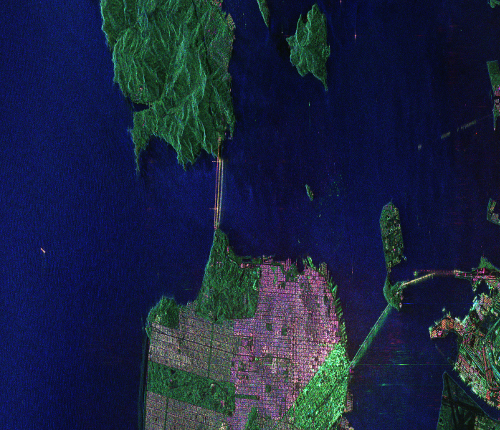
\includegraphics[width=0.7\textwidth]{../Art/visuPauli.png}
\itkcaption[SAR polarimetry visu]{RGB image obtained from Pauli decomposition (sensor : RADARSAT2).}
\label{fig:colorfrisco}
\end{figure}

\section{Image processing and information extraction}\label{sec:improc}

\subsection{Simple calculus with channels}\label{ssec:calculus}

The Band Math application, \textbf{otbBandMath-cli}, provides a simple and efficient way to perform band operations. The command line application and the corresponding Monteverdi module (shown in the section \ref{Band_math module}) are based on the same standards. It computes a band wise operation according to a user defined mathematical expression. The following code computes the absolute difference between first bands of two images:

\begin{verbatim}
otbBandMath-cli -ims input_image_1 input_image_2 
                -exp "abs(im1b1 - im2b1)"
                -out output_image
\end{verbatim}

The naming convention "im[x]b[y]" designates the yth band of the xth input image.

The Band Math application embeds built-in operators and functions (listed \href{http://muparser.sourceforge.net/mup_features.html#idDef2}{here}), allowing a vast choice of possible operations. 

\subsection{Classification}\label{ssec:classification}

The aim of the new SVM classification framework is to provide a supervised pixel-wise classification chain based on learning from multiple images. It supports huge images through streaming and multi-threading.
The classification chain will perform a SVM training step based on the intensities of each pixel as features. Please note that the images will have the same number of bands to be comparable.

\subsubsection{Statistics estimation}
In order to make these features comparable between each images, the first step is to estimate the input images statistics. These statistics will be used to center and reduce the intensities (mean of 0, standard deviation of 1) of samples based on the vector data produced by the user. To do so, the \textbf{otbEstimateImagesStatistics} tool can be used :

\begin{verbatim}
otbEstimateImagesStatistics-cli -in  list_of_input_images 
                                -out statistics.xml
\end{verbatim}

This tool will compute each band mean, compute the standard deviation based on pooled variance of each band and finally export them to an XML file.

The features statistics XML file will be an input of the following tools. 

\subsubsection{Building a training data set}

The chain is supervised : one has to build a training set with positive examples of different objects of interest. This can be done with Monteverdi Vectorization module (Fig.\ref{fig:vectoModuleDataSetCreation}), by building a VectorData containing polygons centered on occurrences of the different objects of interest. This operation will be reproduced on each image used as input of the training function.

Please note that the positive examples in the vector data should have a Class field with a label higher than 1 and coherent in each different images. 

\begin{figure}
  \center
  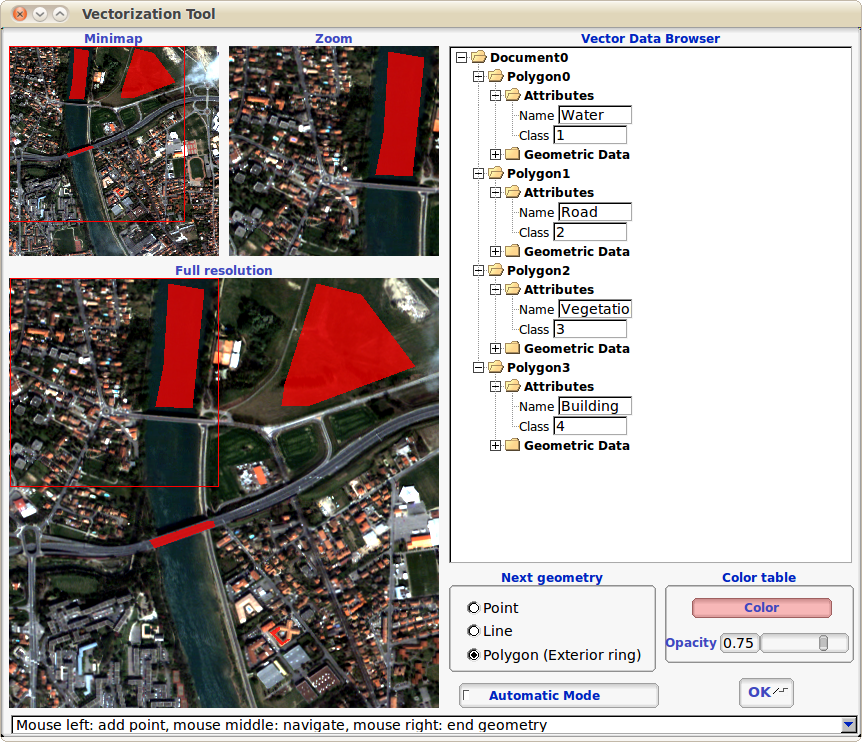
\includegraphics[width=1\textwidth]{../Art/MonteverdiImages/monteverdi_vectorization_module_for_classification.png}
  \itkcaption[GUI of the vectorization module with data for classification chain]{A training data set builded with the vectorization monteverdi module.}
  \label{fig:vectoModuleDataSetCreation}
\end{figure}

You can generate the vector data set with QGIS software for example. The \app should be able to transform the vectordata into the image coordinate system. 

\subsubsection{Training data set}

Once images statistics have been estimated, the learning scheme is the following:
\begin{enumerate}
  \item For each input image:
  \begin{enumerate}
    \item Read the region of interest (ROI) inside the shapefile,
    \item Generate validation and training data within the ROI,
    \item Add the vectors respectively to the training samples set and the validation samples set.
  \end{enumerate}
  \item Increase the size of the training samples set and balance it by generating new noisy samples from the previous ones,
  \item SVM learning with this training set
  \item Performances estimation of the SVM classifier on the validation samples set (confusion matrix, precision, recall).
\end{enumerate}

These steps can be performed by the \textbf{otbTrainImagesClassifier} command-line using the following:

\begin{verbatim}
otbTrainImagesClassifier-cli -is  images_statistics.xml 
                             -in  list_of_input_images 
                             -vd  list_of_positive_examples_shapefiles
                             -out model.svm
                             -b
\end{verbatim}

Some options are available:
\begin{itemize}
\item -dem \textit{a DEM directory to keep accurate the vectordata reprojection}
\item -m   \textit{margin value}
\item -k   \textit{svm kernel (0 = LINEAR (default), 1 = RBF,  2 = POLY, 3 = SIGMOID) }
\item -opt \textit{use svm parameters optimization}
\item -mt  \textit{maximum training samples size} 
\item -mv  \textit{maximum validation samples size}
\item -vrt \textit{ratio validation training}
\end{itemize}

\subsubsection{Validate the classification model}
It is also possible to estimate the SVM model performance with a new validation sample set and another image with the following application.
It will compute the global confusion matrix and precision, recall and F-score of each class based on the \href{http://www.orfeo-toolbox.org/doxygen-current/classotb_1_1ConfusionMatrixCalculator.html}{ConfusionMatrixCalculator} class.
It is done by \textbf{otbValidateImagesClassifier}:

\begin{verbatim}
otbValidateImagesClassifier-cli -is  images_statistics.xml
                                -svm model.svm
                                -in  input_image
                                -vd  list_of_positive_examples_shapefiles
\end{verbatim}

You can save these results with the option -out output filename. You can also set a DEM repository (-dem) to keep the vectordata reprojection accurate.

\subsubsection{Using the classification model} 
Once the classifier has been trained, one can apply the model to classify pixel inside defined classes on a new image using the \textbf{otbImageSVMClassifier} tool:

\begin{verbatim}
 otbImageSVMClassifier-cli -is  images_statistics.xml
                           -svm model.svm 
                           -in  input_image
                           -out labeled_image
\end{verbatim}

You can set an input mask to limit the classification to the mask area with value \textgreater 0.

\subsubsection{Fancy classification results}

In order to get an RGB classification map instead of greylevel labels, one can use the \textbf{otbLabeledImageColorMapping} tool. This tool will replace each label with an 8-bits RGB color specificied in a mapping file. The mapping file should look like this :

\begin{verbatim}
# Lines beginning with a # are ignored
1 255 0 0
\end{verbatim}

In the previous example, 1 is the label and 255 0 0 is a RGB color (this one will be rendered as red). To use the mapping tool, enter the following :

\begin{verbatim}
otbLabeledImageColorMapping-cli -in  labeled_image 
                                -out color_image
                                -ct  mapping_file
\end{verbatim}

\subsubsection{Example}
We take 4 classes: water, roads, vegetation and buildings with red roof.
Data are available in the OTB-Data \href{http://hg.orfeo-toolbox.org/OTB-Data/file/0fed8f4f035c/Input/Classification}{repository} and this image is produced with the commands inside this \href{http://hg.orfeo-toolbox.org/OTB-Applications/file/3ce975605013/Testing/Classification/CMakeLists.txt}{file}. 

\begin{figure}[!h]
  \center
  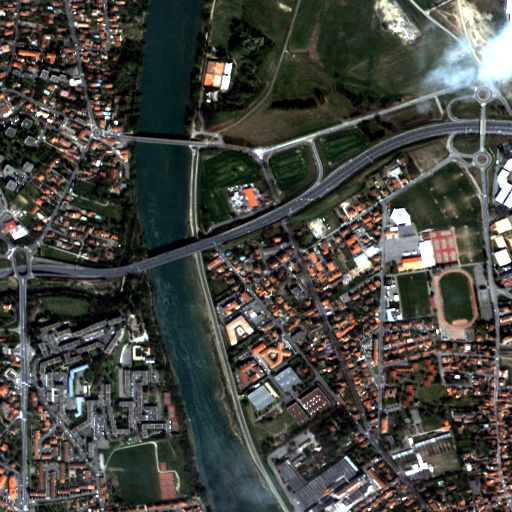
\includegraphics[width=0.3\textwidth]{../Art/MonteverdiImages/classification_chain_inputimage.jpg}
  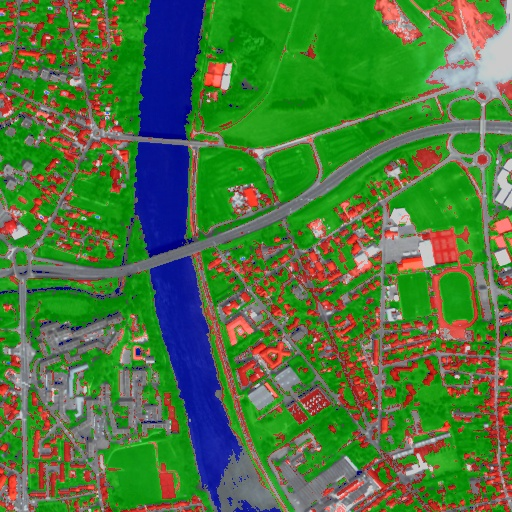
\includegraphics[width=0.3\textwidth]{../Art/MonteverdiImages/classification_chain_fancyclassif_fusion.jpg}
  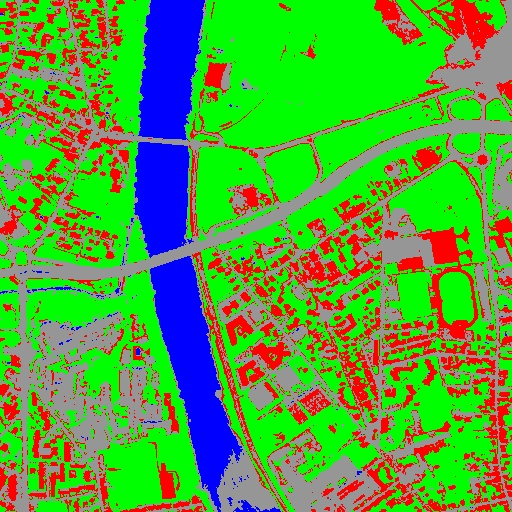
\includegraphics[width=0.3\textwidth]{../Art/MonteverdiImages/classification_chain_fancyclassif.jpg}}
  \itkcaption[ExampleSVMCalssif]{From left to right: Original image, result image with fusion (with monteverdi viewer) of original image and fancy classification and input image with fancy color classification from labeled image.}
  \label{fig:MeanShiftVectorImageFilter}
\end{figure}



%\subsection{Segmentation}\label{ssec:segmentation}
%todo.

%\subsection{Change detection}\label{ssec:changedetection}
%todo.

%\subsection{Object-based image analysis}\label{ssec:obia}
%todo.

\subsection{Dempster Shafer based Classifier Fusion}\label{ssec:classifierfusion}

This framework is dedicated to, starting from the result of a detection (for example a road extraction), enhance the results fiability by using a classifier fusion based validation algorithm. Using a set of descriptors, the processing chain validates or invalidates the input geometrical features.

\subsubsection{Prequel: Road Extraction}

The first step of this recipe is to produce an interesting and adapted input. The \textbf{otbRoadExtractionApplication},  included in the \app package, provides a set of geometrical features that can be used as input of the following process. This is only an example, the Dempster-Shafer framework was not designed specificaly to be used with \textbf{otbRoadExtractionApplication} but it is a good example of what the input should be like.

\subsubsection{Fuzzy Model (requisite)}

Perform the fuzzy model estimation (once by use case: descriptor set / Belief support / Plausibility support).
Inputs:
\begin{itemize}
\item a vector data of positive samples enriched according to the "Compute Descriptors" part
\item a vector data of negative samples enriched according to the "Compute Descriptors" part
\item a support for the Belief computation
\item a support for the Plausibility computation
\item a initialization model (xml file) or a descriptor name list (listing the descriptors to be included in the model)
\end{itemize}
Output:
\begin{itemize}
\item a FuzzyModel.xml file containing the model
\end{itemize}
Usage:

\begin{verbatim}
 otbDSFuzzyModelEstimation-cli -psin     PosSamples.shp 
                               -nsin     NegSamples.shp 
                               -BelSup   "ROADSA" 
                               -PlaSup   "NONDVI" "ROADSA" "NOBUIL" 
                               -DescList "NONDVI" "ROADSA" "NOBUIL" 
                               -out      FuzzyModel.xml
\end{verbatim}

FuzzyModel.xml contains the optimal model to perform the classifier fusion.

\subsubsection{First Step: Compute Descriptors}

The First step in the classifier fusion based validation is to compute, for every studied polyline, the choosen descriptors. In this context, the \textbf{otbComputePolylineFeatureFromImage} application can be used for a large panel of descriptors.
Inputs:
\begin{itemize}
\item an image (of the sudied scene) corresponding to the choosen descriptor (NDVI, building Mask\dots)
\item a vector data containing polyline of interest
\item a formula ("b1 \textgreater 0.4", "b1 == 0") where b1 is the standard name of input image first band
\item a field name corresponding to the descriptor codename (NONDVI, ROADSA...)
\end{itemize}
Output:
\begin{itemize}
\item a vector data containing polylines with a new field containing the descriptor value
\end{itemize}
Usage: To add the "NONDVI" descriptor to an input VectorData ("inVD.shp") corresponding to the percentage of pixel along a polyline that verifies the formula that have a NDVI \textgreater 0.4 :

\begin{verbatim}
 otbComputePolylineFeatureFromImage-cli -img   NDVI.TIF 
                                        -vdin  inVD.shp 
                                        -expr  "b1 > 0.4" 
                                        -field "NONDVI" 
                                        -out   VD_NONDVI.shp
\end{verbatim}

where NDVI.TIF is the ndvi mono band image of the studied scene.
This step must be repeated for each choosen descriptor

\begin{verbatim}
 otbComputePolylineFeatureFromImage-cli -img   roadSpectralAngle.TIF  
                                        -vdin  VD_NONDVI.shp 
                                        -expr  "b1 > 0.24"
                                        -field "ROADSA" 
                                        -out   VD_NONDVI_ROADSA.shp
\end{verbatim}

\begin{verbatim}
 otbComputePolylineFeatureFromImage-cli -img   Buildings.TIF 
                                        -vdin  VD_NONDVI_ROADSA.shp 
                                        -expr  "b1 == 0" 
                                        -field "NOBUILDING" 
                                        -out   VD_NONDVI_ROADSA_NOBUIL.shp
\end{verbatim}

Both NDVI.TIF and roadSpectralAngle.TIF can be produced using Monteverdi Feature Extraction capabilites, and Buildings.TIF can be generated using Monteverdi Rasterization module.
From now on, VD\_NONDVI\_ROADSA\_NOBUIL.shp contains three descriptor fields. It will be used in the following parts.

\subsubsection{Second Step: Feature Validation}

The final application which, using the Dempster-Shafer theory, will validate or unvalidate the studied samples
Inputs:
\begin{itemize}
\item an enriched vector data VD\_NONDVI\_ROADSA\_NOBUIL.shp
\item a support for the Belief computation
\item a support for the Plausibility computation
\item a fuzzy model FuzzyModel.xml
\end{itemize}
Output:
\begin{itemize}
\item a vector data containing only the validated samples
\end{itemize}
\begin{verbatim}
 otbVectorDataDSValidation-cli -in      extractedRoads_enriched.shp 
                               -descMod FuzzyModel.xml 
                               -out     validatedSamples.shp
\end{verbatim}


\section{Classification}\label{sec:classification}

\subsection{Pixel based classification}\label{ssec:pbclassif}

The classification in the application framework provides a supervised pixel-wise
classification chain based on learning from multiple images, and using one 
specified machine learning method like SVM, Bayes, KNN, Random Forests, Artificial 
Neural Network, and others...(see application help of 
\application{TrainImagesClassifier} for further details about all the available 
classifiers). It supports huge images through streaming and multi-threading. The 
classification chain performs a training step based on the intensities of each 
pixel as features. Please note that all the input images must have the same number 
of bands to be comparable.

\subsubsection{Statistics estimation}
In order to make these features comparable between each training images, the first 
step consists in estimating the input images statistics. These statistics will be 
used to center and reduce the intensities (mean of 0 and standard deviation of 1) 
of samples based on the vector data produced by the user. To do so, the
\application{ComputeImagesStatistics} tool can be used:

\begin{verbatim}
otbcli_ComputeImagesStatistics -il  im1.tif im2.tif im3.tif
                               -out images_statistics.xml
\end{verbatim}

This tool will compute each band mean, compute the standard deviation based on
pooled variance of each band and finally export them to an XML file.
The features statistics XML file will be an input of the following tools.

\subsubsection{Building the training data set}

As the chain is supervised, we first need to build a training set with
positive examples of different objects of interest. This can be done
with Monteverdi Vectorization module
(Fig.\ref{fig:vectoModuleDataSetCreation}).
These polygons must be saved in OGR vector format supported
by GDAL like ESRI shapefile for example.

This operation will be reproduced on each image used as input of the training
function.

Please note that the positive examples in the vector data should have a ``Class``
field with a label value higher than 1 and coherent in each images.

\begin{figure}
  \center
  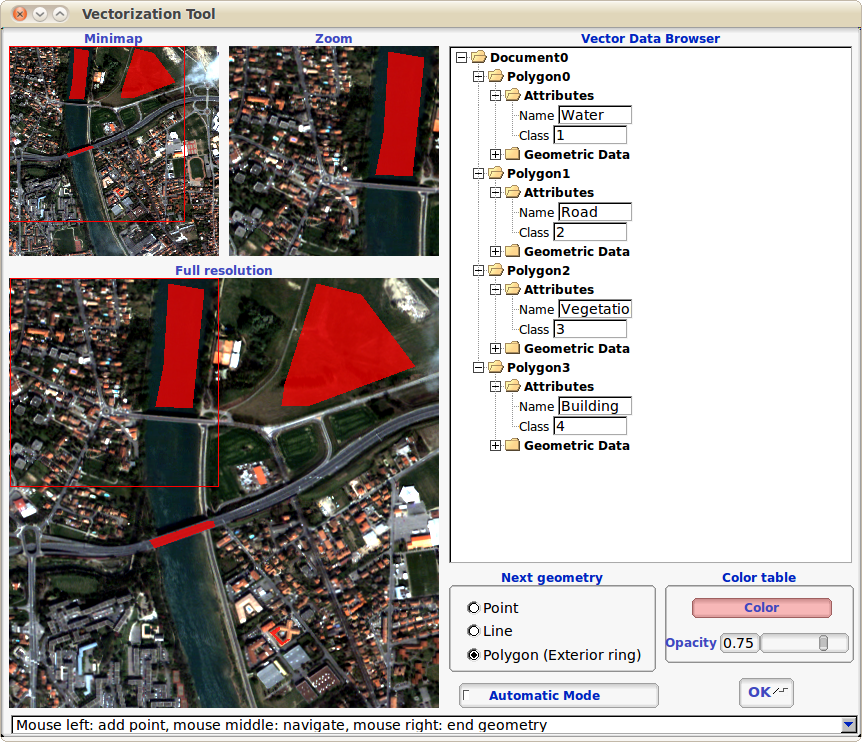
\includegraphics[width=1\textwidth]{../Art/MonteverdiImages/monteverdi_vectorization_module_for_classification.png}
  \itkcaption[GUI of the vectorization module with data for classification chain]{A training data set builded with the vectorization monteverdi module.}
  \label{fig:vectoModuleDataSetCreation}
\end{figure}

You can generate the vector data set with \qgis software for
example and save it in an OGR vector format supported by \gdal (ESRI
sphapefile for example). \app should be able to transform the
vector data into the image coordinate system.

\subsubsection{Performing the learning scheme}

Once images statistics have been estimated, the learning scheme is the following:
\begin{enumerate}
  \item For each input image:
  \begin{enumerate}
    \item Read the region of interest (ROI) inside the shapefile,
    \item Generate validation and training data within the ROI,
    \item Add vectors respectively to the training samples set and the validation
    samples set.
  \end{enumerate}
  \item Increase the size of the training samples set and balance it by
  generating new noisy samples from the previous ones,
  \item Perform the learning with this training set
  \item Estimate performances of the classifier on the validation samples set
  (confusion matrix, precision, recall and F-Score).
\end{enumerate}

Let us consider a SVM classification. These steps can be performed by the 
\application{TrainImagesClassifier} command-line using the following:

\begin{verbatim}
otbcli_TrainImagesClassifier -io.il      im1.tif im2.tif im3.tif
                             -io.vd      vd1.shp vd2.shp vd3.shp
                             -io.imstat  images_statistics.xml
                             -classifier svm (classifier_for_the_training)
                             -io.out     model.svm
\end{verbatim}

Additional groups of parameters are also available (see application help for
more details):
\begin{itemize}
\item \verb?-elev? Handling of elevation (DEM or average elevation)
\item \verb?-sample? Group of parameters for sampling
\item \verb?-classifier? Classifiers to use for the training, and their corresponding groups of parameters
\end{itemize}


\subsubsection{Using the classification model}
Once the classifier has been trained, one can apply the model to classify
pixel inside defined classes on a new image using the
\application{ImageClassifier} application:

\begin{verbatim}
otbcli_ImageClassifier -in     image.tif
                       -imstat images_statistics.xml
                       -model  model.svm
                       -out    labeled_image.tif
\end{verbatim}

You can set an input mask to limit the classification to the mask area with
value \textgreater 0.


\subsubsection{Validating the classification model}
The performance of the model generated by the \application{TrainImagesClassifier} 
application is directly estimated by the application itself, which displays the 
precision, recall and F-score of each class, and can generate the global confusion 
matrix as an output *.CSV file.
 
With the \application{ConputeConfusionMatrix} application, it is also possible to 
estimate the performance of a model from a classification map generated with the 
\application{ImageClassifier} application. 
This labeled image is compared to positive reference samples (either represented as 
a raster labeled image or as a vector data containing the reference classes). It 
will compute the confusion matrix and precision, recall and F-score of each class 
too, based on the 
\href{http://www.orfeo-toolbox.org/doxygen-current/classotb_1_1ConfusionMatrixCalculator.html}{ConfusionMatrixCalculator} 
class.

\begin{verbatim}
otbcli_ComputeConfusionMatrix -in                labeled_image.tif
                              -ref               vector
                              -ref.vector.in     vectordata.shp
                              -ref.vector.field  Class (name_of_label_field)
                              -out               confusion_matrix.csv
\end{verbatim}


%You can also set a DEM repository (-dem) to keep the vectordata reprojection accurate.

\subsubsection{Fancy classification results}
\label{ssec:classificationcolormapping}
Color mapping can be used to apply color transformations on the final
graylevel label image. It allows to get an RGB classification map
by re-mapping the image values to be suitable for display purposes.
One can use the \application{ColorMapping} application. This tool will
replace each label with an 8-bits RGB color specificied in a mapping
file. The mapping file should look like this :

\begin{verbatim}
# Lines beginning with a # are ignored
1 255 0 0
\end{verbatim}

In the previous example, 1 is the label and 255 0 0 is a RGB color
(this one will be rendered as red). To use the mapping tool, enter
the following :

\begin{verbatim}
otbcli_ColorMapping -in                labeled_image.tif
                    -method            custom
                    -method.custom.lut lut_mapping_file.txt
                    -out               RGB_color_image.tif
\end{verbatim}

Other look-up tables (LUT) are available : standard continuous LUT,
optimal LUT, and LUT computed over a support image.

\subsubsection{Example}

We consider 4 classes: water, roads, vegetation and buildings with red roofs.
Data is available in the OTB-Data
\href{http://hg.orfeo-toolbox.org/OTB-Data/file/0fed8f4f035c/Input/Classification}{repository}
and this image is produced with the commands inside this
\href{http://hg.orfeo-toolbox.org/OTB-Applications/file/3ce975605013/Testing/Classification/CMakeLists.txt}{file}.

\begin{figure}[!h]
  \center
  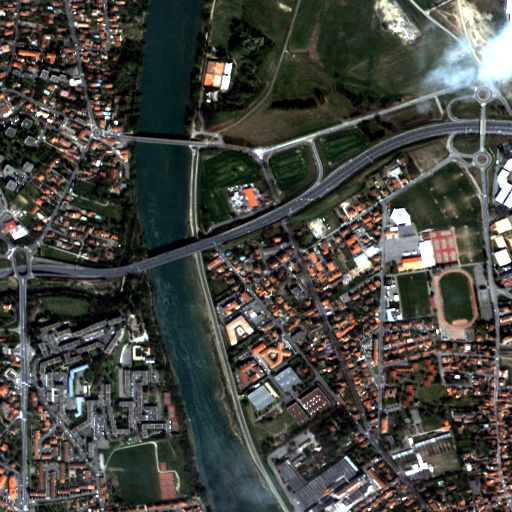
\includegraphics[width=0.3\textwidth]{../Art/MonteverdiImages/classification_chain_inputimage.jpg}
  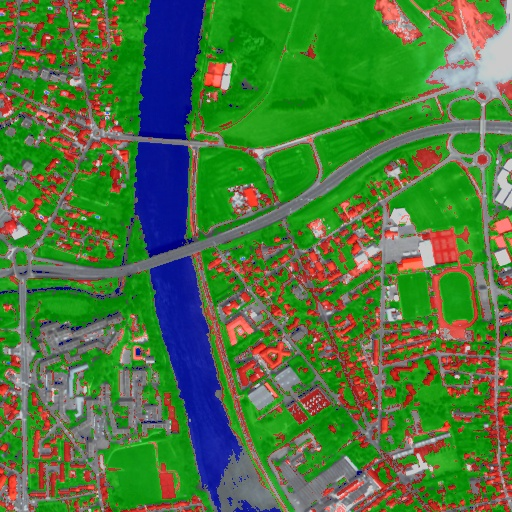
\includegraphics[width=0.3\textwidth]{../Art/MonteverdiImages/classification_chain_fancyclassif_fusion.jpg}
  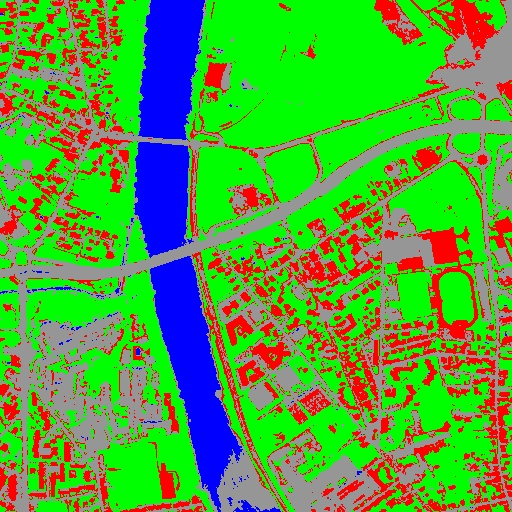
\includegraphics[width=0.3\textwidth]{../Art/MonteverdiImages/classification_chain_fancyclassif.jpg}
  \itkcaption[ExampleSVMClassif]{From left to right: Original image,
    result image with fusion (with monteverdi viewer) of original
    image and fancy classification and input image with fancy color
    classification from labeled image.}
  \label{fig:MeanShiftVectorImageFilter}
\end{figure}




\subsection{Fusion of classification maps}\label{ssec:fusionofclassifications}

After having processed several classifications of the same input image but from 
different models or methods (SVM, KNN, Random Forest,...), it is possible to make a 
fusion of these classification maps with the \application{FusionOfClassifications} 
application which uses either majority voting or the Demspter Shafer framework to 
handle this fusion. The Fusion of Classifications generates a single more robust and 
precise classification map which combines the information extracted from the input 
list of labeled images. 

The \application{FusionOfClassifications} application has the following input parameters :
\begin{itemize}
\item \verb?-il? list of input labeled classification images to fuse
\item \verb?-out? the output labeled image resulting from the fusion of the input classification images
\item \verb?-method? the fusion method (either by majority voting or by Dempster Shafer)
\item \verb?-nodatalabel? label for the no data class (default value = 0)
\item \verb?-undecidedlabel? label for the undecided class (default value = 0)
\end{itemize}


The input pixels with the nodata class label are simply ignored by the fusion process. 
Moreover, the output pixels for which the fusion process does not result in a unique 
class label, are set to the undecided value.

\subsubsection{Majority voting for the fusion of classifications}

In the Majority Voting method implemented in the \application{FusionOfClassifications} 
application, the value of each output pixel is equal to the more frequent class 
label of the same pixel in the input classification maps. However, it may happen 
that the more frequent class labels are not unique in individual pixels. In that 
case, the undecided label is attributed to the output pixels.


The application can be used like this:
\begin{verbatim}
otbcli_FusionOfClassifications  -il             cmap1.tif cmap2.tif cmap3.tif
                                -method         majorityvoting
                                -nodatalabel    0
                                -undecidedlabel 10
                                -out            MVFusedClassificationMap.tif
\end{verbatim}


Let us consider 6 independent classification maps of the same input image (Cf. left 
image in Fig. \ref{fig:MeanShiftVectorImageFilter}) generated from 6 different SVM 
models. The Fig. \ref{fig:ClassificationMapFusionApplication} represents them after 
a color mapping by the same LUT. Thus, 4 classes (water: blue, roads: gray, 
vegetation: green, buildings with red roofs: red) are observable on each of them.


\begin{figure}[!h]
  \center
  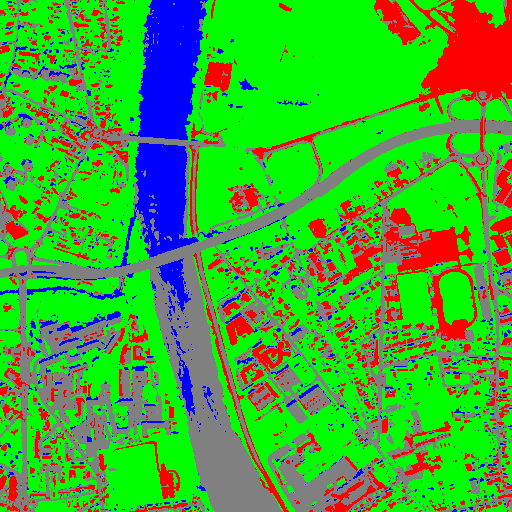
\includegraphics[width=0.3\textwidth]{../Art/MonteverdiImages/QB_1_ortho_C1_CM.png}
  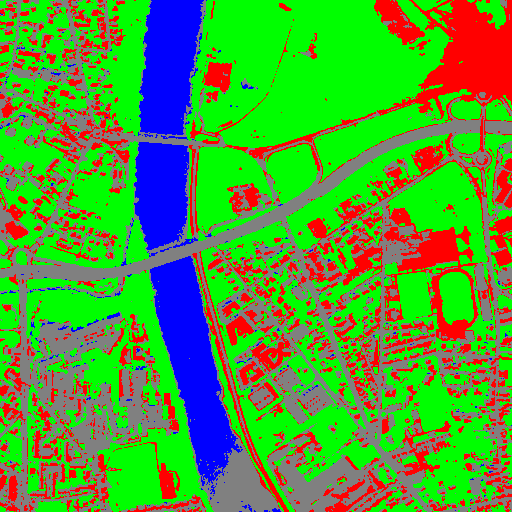
\includegraphics[width=0.3\textwidth]{../Art/MonteverdiImages/QB_1_ortho_C2_CM.png}
  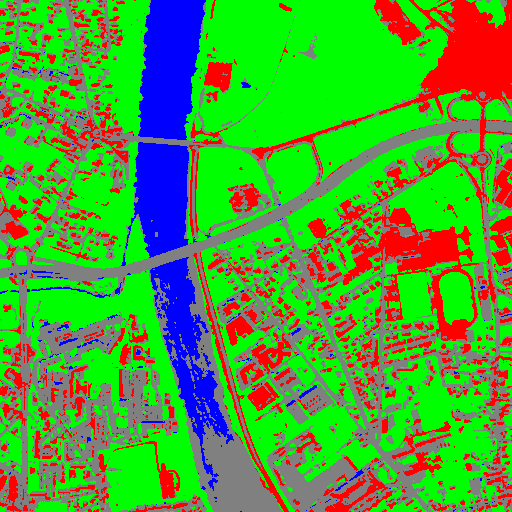
\includegraphics[width=0.3\textwidth]{../Art/MonteverdiImages/QB_1_ortho_C3_CM.png}
  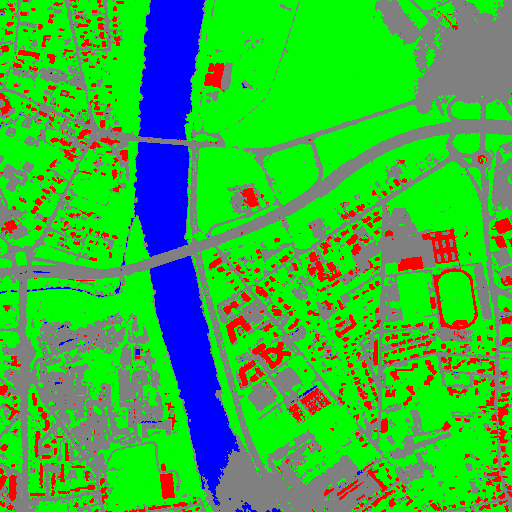
\includegraphics[width=0.3\textwidth]{../Art/MonteverdiImages/QB_1_ortho_C4_CM.png}
  \includegraphics[width=0.3\textwidth]{../Art/MonteverdiImages/QB_1_ortho_C5_CM.png}
  \includegraphics[width=0.3\textwidth]{../Art/MonteverdiImages/QB_1_ortho_C6_CM.png}
  \itkcaption[ExampleSVMClassifFusion]{Six fancy colored classified images to be fused, generated from 6 different SVM models.}
  \label{fig:ClassificationMapFusionApplication}
\end{figure}


As an example of the \application{FusionOfClassifications} application by 
\emph{majority voting}, the fusion of the six input classification maps 
represented in Fig. \ref{fig:ClassificationMapFusionApplication} leads to the 
classification map illustrated on the right in Fig. \ref{fig:ClassificationMapFusionApplicationMV}. 
Thus, it appears that this fusion highlights the more relevant classes among the six  
different input classifications. The white parts of the fused image correspond to 
the undecided class labels, i.e. to pixels for which there is not a unique 
majority voting.


\begin{figure}[!h]
  \center
  \includegraphics[width=0.3\textwidth]{../Art/MonteverdiImages/classification_chain_inputimage.jpg}
  \includegraphics[width=0.3\textwidth]{../Art/MonteverdiImages/QB_1_ortho_MV_C123456_CM.png}
  \itkcaption[ExampleSVMClassifFusionMV]{From left to right: Original image, and fancy colored classified image obtained by a 
  majority voting fusion of the 6 classification maps represented in Fig. \ref{fig:ClassificationMapFusionApplication} (water: blue, roads: gray, 
vegetation: green, buildings with red roofs: red, undecided: white).}
  \label{fig:ClassificationMapFusionApplicationMV}
\end{figure}


\subsubsection{Dempster Shafer framework for the fusion of classifications}

The \application{FusionOfClassifications} application, handles another method to 
compute the fusion: the Dempster Shafer framework. 
In the \href{http://en.wikipedia.org/wiki/Dempster-Shafer\_theory}{Dempster-Shafer theory}, 
the performance of each classifier resulting in the classification maps to fuse are 
evaluated with the help of the so-called \emph{belief function} of each class label, 
which measures the degree of belief that the corresponding label is correctly assigned 
to a pixel. For each classifier, and for each class label, these belief
functions are estimated from another parameter called the \emph{mass of belief} of each class label, 
which measures the confidence that the user can have in each classifier according to 
the resulting labels.

In the Dempster Shafer framework for the fusion of classification maps, the fused 
class label for each pixel is the one with the maximal belief function. In case of 
multiple class labels maximizing the belief functions, the output fused pixels are 
set to the undecided value.

In order to estimate the confidence level in each classification map, each of them 
should be confronted with a ground truth. For this purpose, the masses of belief of 
the class labels resulting from a classifier are estimated from its confusion 
matrix, which is itself exported as a *.CSV file with the help of the 
\application{ComputeConfusionMatrix} application. Thus, using the Dempster Shafer 
method to fuse classification maps needs an additional input list of such *.CSV files 
corresponding to their respective confusion matrices.

The application can be used like this:
\begin{verbatim}
otbcli_FusionOfClassifications  -il             cmap1.tif cmap2.tif cmap3.tif
                                -method         dempstershafer
                                -method.dempstershafer.cmfl
                                                cmat1.csv cmat2.csv cmat3.csv
                                -nodatalabel    0
                                -undecidedlabel 10
                                -out            DSFusedClassificationMap.tif
\end{verbatim}



As an example of the \application{FusionOfClassifications} application by 
\emph{Dempster Shafer}, the fusion of the six input classification maps 
represented in Fig. \ref{fig:ClassificationMapFusionApplication} leads to the 
classification map illustrated on the right in Fig. \ref{fig:ClassificationMapFusionApplicationDS}. 
Thus, it appears that this fusion gives access to a more precise and robust 
classification map based on the confidence level in each classifier.


\begin{figure}[!h]
  \center
  \includegraphics[width=0.3\textwidth]{../Art/MonteverdiImages/classification_chain_inputimage.jpg}
  \includegraphics[width=0.3\textwidth]{../Art/MonteverdiImages/QB_1_ortho_DS_V_P_C123456_CM.png}
  \itkcaption[ExampleSVMClassifFusionDS]{From left to right: Original image, and fancy colored classified image obtained by a 
  Dempster Shafer fusion of the 6 classification maps represented in Fig. \ref{fig:ClassificationMapFusionApplication} (water: blue, roads: gray, 
vegetation: green, buildings with red roofs: red, undecided: white).}
  \label{fig:ClassificationMapFusionApplicationDS}
\end{figure}
 

\subsubsection{Recommandations to properly use the fusion of classification maps}

In order to properly use the \application{FusionOfClassifications} application, 
some points should be considered. First, the \verb?list_of_input_images? and 
\verb?OutputFusedClassificationImage? are single band labeled images, which means 
that the value of each pixel corresponds to the class label it belongs to, and 
labels in each classification map must represent the same class. Secondly, the 
undecided label value must be different from existing labels in the input images in 
order to avoid any ambiguity in the interpretation of the \verb?OutputFusedClassificationImage?.





\subsection{Majority voting based classification map regularization}\label{ssec:classificationmapregularization}

Resulting classification maps can be regularized in order to smoothen irregular classes. Such a regularization process
improves classification results by making more homogeneous areas which are easier to handle.

\subsubsection{Majority voting for the classification map regularization}

The \application{ClassificationMapRegularization} application performs a regularization of a labeled input image
based on the Majority Voting method in a specified ball shaped neighborhood. For each center pixel, Majority Voting takes the
more representative value of all the pixels identified by the structuring element and then sets the output center pixel
to this majority label value. The ball shaped neighborhood is identified by its radius expressed in pixels.


\subsubsection{Handling ambiguity and not classified pixels in the majority voting based regularization}

Since, the Majority Voting regularization may lead to not unique majority labels in the neighborhood, it is important to define
which behaviour the filter must have in this case. For this purpose, a Boolean parameter (called ip.suvbool) is used in the
\application{ClassificationMapRegularization} application to choose whether pixels with more than one majority class are set to
Undecided (true), or to their Original labels (false = default value).

Moreover, it may happen that pixels in the input image do not belong to any of the considered class. Such pixels are
assumed to belong to the NoData class, the label of which is specified as an input parameter for the regularization. Therefore,
those NoData input pixels are invariant and keep their NoData label in the output regularized image.
 
The \application{ClassificationMapRegularization} application has the following input parameters :
\begin{itemize}
\item \verb?-io.in? labeled input image resulting from a previous classification process
\item \verb?-io.out? output labeled image corresponding to the regularization of the input image
\item \verb?-ip.radius? integer corresponding to the radius of the ball shaped structuring element (default value = 1 pixel)
\item \verb?-ip.suvbool? boolean parameter used to choose whether pixels with more than one majority class are set to Undecided (true),
or to their Original labels (false = default value). Please note that the Undecided value must be different from existing labels in the input image
\item \verb?-ip.nodatalabel? label for the NoData class. Such input pixels keep their NoData label in the output image (default value = 0)
\item \verb?-ip.undecidedlabel? label for the Undecided class (default value = 0).
\end{itemize}


The application can be used like this:
\begin{verbatim}
otbcli_ClassificationMapRegularization  -io.in              labeled_image.tif
                                        -ip.radius          3
                                        -ip.suvbool         true
                                        -ip.nodatalabel     10
                                        -ip.undecidedlabel  7
                                        -io.out             regularized.tif
\end{verbatim}
 

\subsubsection{Recommandations to properly use the majority voting based regularization}

In order to properly use the \application{ClassificationMapRegularization} application, some points should be considered.
First, both \verb?InputLabeledImage? and \verb?OutputLabeledImage? are single band labeled images, which means that the
value of each pixel corresponds to the class label it belongs to. The \verb?InputLabeledImage? is commonly an image generated
with a classification algorithm such as the SVM classification. Remark: both
\verb?InputLabeledImage? and \verb?OutputLabeledImage? are not necessarily of the same datatype. Secondly, if ip.suvbool == true,
the Undecided label value must be different from existing labels in the input labeled image in order to avoid any ambiguity in the
interpretation of the regularized \verb?OutputLabeledImage?. Finally, the structuring element radius must have a minimum value equal to 1 pixel,
which is its default value. Both NoData and Undecided labels have a default value equal to 0.


\subsubsection{Example}

Resulting from the \application{ColorMapping} application presented in section \ref{ssec:classificationcolormapping}, and illustrated in
Fig. \ref{fig:MeanShiftVectorImageFilter}, the Fig. \ref{fig:ClassificationMapRegularizationApplication} shows a regularization of a classification
map composed of 4 classes: water, roads, vegetation and buildings with red roofs. The radius of the ball shaped structuring element is equal to 3 pixels,
which corresponds to a ball included in a 7 x 7 pixels square. Pixels with more than one majority class keep their original labels.

\begin{figure}[!h]
  \center
  \includegraphics[width=0.3\textwidth]{../Art/MonteverdiImages/classification_chain_inputimage.jpg}
  \includegraphics[width=0.3\textwidth]{../Art/MonteverdiImages/classification_chain_fancyclassif_CMR_input.png}
  \includegraphics[width=0.3\textwidth]{../Art/MonteverdiImages/classification_chain_fancyclassif_CMR_3.png}
  \itkcaption[ExampleSVMClassifCMR]{From left to right: Original image, fancy colored classified image and regularized classification map with radius equal to 3 pixels.}
  \label{fig:ClassificationMapRegularizationApplication}
\end{figure}


\section{Feature extraction}\label{sec:featextract}

As described in the OTB Software Guide, the term {\em Feature Extraction} refers to
techniques aiming at extracting added value information from images. These
extracted items named {\em features} can be local statistical moments, edges,
radiometric indices, morphological and textural properties. For example, such
features can be used as input data for other image processing methods like
{\em Segmentation} and {\em Classification}.

\subsection{Local statistics extraction}\label{ssec:localstatextraction}

This application computes the 4 local statistical moments on every pixel in the
selected channel of the input image, over a specified neighborhood. The output
image is multi band with one statistical moment (feature) per band. Thus, the 4
output features are the Mean, the Variance, the Skewness and the Kurtosis. They are
provided in this exact order in the output image.


The \application{LocalStatisticExtraction} application has the following input parameters:
\begin{itemize}
\item \verb?-in? the input image to compute the features on
\item \verb?-channel? the selected channel index in the input image to be processed (default value is 1)
\item \verb?-radius? the computational window radius (default value is 3 pixels)
\item \verb?-out? the output image containing the local statistical moments
\end{itemize}


The application can be used like this:
\begin{verbatim}
otbcli_LocalStatisticExtraction  -in        InputImage
                                 -channel   1
                                 -radius    3
                                 -out       OutputImage
\end{verbatim}



\subsection{Edge extraction}\label{ssec:edgeextraction}

This application Computes edge features on every pixel in the selected channel
of the input image.

The \application{EdgeExtraction} application has the following input parameters:
\begin{itemize}
\item \verb?-in? the input image to compute the features on
\item \verb?-channel? the selected channel index in the input image to be processed (default value is 1)
\item \verb?-filter? the choice of edge detection method (gradient/sobel/touzi) (default value is gradient)
~~\\
\item \verb?(-filter.touzi.xradius)? the X Radius of the Touzi processing neighborhood (only if filter==touzi) (default value is 1 pixel)
\item \verb?(-filter.touzi.yradius)? the Y Radius of the Touzi processing neighborhood (only if filter==touzi) (default value is 1 pixel)
~~\\
\item \verb?-out? the output mono band image containing the edge features
\end{itemize}


The application can be used like this:
\begin{verbatim}
otbcli_EdgeExtraction  -in        InputImage
                       -channel   1
                       -filter    sobel
                       -out       OutputImage
\end{verbatim}

or like this if filter==touzi:

\begin{verbatim}
otbcli_EdgeExtraction  -in                    InputImage
                       -channel               1
                       -filter                touzi
                       -filter.touzi.xradius  2
                       -filter.touzi.yradius  2 
                       -out                   OutputImage
\end{verbatim}




\subsection{Radiometric indices extraction}\label{ssec:Radiomindextraction}

This application computes radiometric indices using the channels of the input
image. The output is a multi band image into which each channel is one of
the selected indices.


The \application{RadiometricIndices} application has the following input parameters:
\begin{itemize}
\item \verb?-in? the input image to compute the features on
\item \verb?-out? the output image containing the radiometric indices
\item \verb?-channels.blue? the Blue channel index in the input image (default value is 1)
\item \verb?-channels.green? the Green channel index in the input image (default value is 1)
\item \verb?-channels.red? the Red channel index in the input image (default value is 1)
\item \verb?-channels.nir? the Near Infrared channel index in the input image (default value is 1)
\item \verb?-channels.mir? the Mid-Infrared channel index in the input image (default value is 1)
\item \verb?-list? the list of available radiometric indices (default value is Vegetation:NDVI)
\end{itemize}

The available radiometric indices to be listed into -list with their relevant
channels in brackets are:

\begin{verbatim}
Vegetation:NDVI - Normalized difference vegetation index (Red, NIR)
Vegetation:TNDVI - Transformed normalized difference vegetation index (Red, NIR)
Vegetation:RVI - Ratio vegetation index (Red, NIR)
Vegetation:SAVI - Soil adjusted vegetation index (Red, NIR)
Vegetation:TSAVI - Transformed soil adjusted vegetation index (Red, NIR)
Vegetation:MSAVI - Modified soil adjusted vegetation index (Red, NIR)
Vegetation:MSAVI2 - Modified soil adjusted vegetation index 2 (Red, NIR)
Vegetation:GEMI - Global environment monitoring index (Red, NIR)
Vegetation:IPVI - Infrared percentage vegetation index (Red, NIR)

Water:NDWI - Normalized difference water index (Gao 1996) (NIR, MIR)
Water:NDWI2 - Normalized difference water index (Mc Feeters 1996) (Green, NIR)
Water:MNDWI - Modified normalized difference water index (Xu 2006) (Green, MIR)
Water:NDPI - Normalized difference pond index (Lacaux et al.) (MIR, Green)
Water:NDTI - Normalized difference turbidity index (Lacaux et al.) (Red, Green)

Soil:RI - Redness index (Red, Green)
Soil:CI - Color index (Red, Green)
Soil:BI - Brightness index (Red, Green)
Soil:BI2 - Brightness index 2 (NIR, Red, Green)
\end{verbatim}

The application can be used like this, which leads to an output image with 3 bands,
respectively with the Vegetation:NDVI, Vegetation:RVI and Vegetation:IPVI
radiometric indices in this exact order:

\begin{verbatim}
otbcli_RadiometricIndices -in             InputImage
                          -out            OutputImage
                          -channels.red   3
                          -channels.green 2
                          -channels.nir   4
                          -list           Vegetation:NDVI Vegetation:RVI
                                          Vegetation:IPVI 
\end{verbatim}


or like this, which leads to a single band output image with the Water:NDWI2 radiometric indice:
\begin{verbatim}
otbcli_RadiometricIndices -in             InputImage
                          -out            OutputImage
                          -channels.red   3
                          -channels.green 2
                          -channels.nir   4
                          -list           Water:NDWI2 
\end{verbatim}

        




\subsection{Morphological features extraction}\label{ssec:morphofeatextraction}

Morphological features can be highlighted by using image filters based on
mathematical morphology either on binary or gray scale images.

\subsubsection{Binary morphological operations}

This application performs binary morphological operations (dilation, erosion,
opening and closing) on a mono band image with a specific structuring element (a
ball or a cross) having one radius along X and another one along Y. NB: the cross
shaped structuring element has a fixed radius equal to 1 pixel in both X and Y
directions.

The \application{BinaryMorphologicalOperation} application has the following input parameters:
\begin{itemize}
\item \verb?-in? the input image to be filtered
\item \verb?-channel? the selected channel index in the input image to be processed (default value is 1)
\item \verb?-structype? the choice of the structuring element type (ball/cross) (default value is ball)
\item \verb?(-structype.ball.xradius)? the ball structuring element X Radius (only if structype==ball) (default value is 5 pixels)
\item \verb?(-structype.ball.yradius)? the ball structuring element Y Radius (only if structype==ball) (default value is 5 pixels)
\item \verb?-filter? the choice of the morphological operation (dilate/erode/opening/closing) (default value is dilate)
\item \verb?(-filter.dilate.foreval)? the foreground value for the dilation (idem for filter.erode/opening/closing) (default value is 1)
\item \verb?(-filter.dilate.backval)? the background value for the dilation (idem for filter.erode/opening/closing) (default value is 0)
\item \verb?-out? the output filtered image
\end{itemize}


The application can be used like this:
\begin{verbatim}
otbcli_BinaryMorphologicalOperation  -in                     InputImage
                                     -channel                1
                                     -structype              ball
                                     -structype.ball.xradius 10
                                     -structype.ball.yradius 5
                                     -filter                 opening
                                     -filter.opening.foreval 1.0
                                     -filter.opening.backval 0.0
                                     -out                    OutputImage
\end{verbatim}





\subsubsection{Gray scale morphological operations}

This application performs morphological operations (dilation, erosion,
opening and closing) on a gray scale mono band image with a specific structuring
element (a ball or a cross) having one radius along X and another one along Y. NB:
the cross shaped structuring element has a fixed radius equal to 1 pixel in both X
and Y directions.

The \application{GrayScaleMorphologicalOperation} application has the following input parameters:
\begin{itemize}
\item \verb?-in? the input image to be filtered
\item \verb?-channel? the selected channel index in the input image to be processed (default value is 1)
\item \verb?-structype? the choice of the structuring element type (ball/cross) (default value is ball)
\item \verb?(-structype.ball.xradius)? the ball structuring element X Radius (only if structype==ball) (default value is 5 pixels)
\item \verb?(-structype.ball.yradius)? the ball structuring element Y Radius (only if structype==ball) (default value is 5 pixels)
\item \verb?-filter? the choice of the morphological operation (dilate/erode/opening/closing) (default value is dilate)
\item \verb?-out? the output filtered image
\end{itemize}


The application can be used like this:
\begin{verbatim}
otbcli_GrayScaleMorphologicalOperation  -in                     InputImage
                                        -channel                1
                                        -structype              ball
                                        -structype.ball.xradius 10
                                        -structype.ball.yradius 5
                                        -filter                 opening
                                        -out                    OutputImage
\end{verbatim}



\subsection{Textural features extraction}\label{ssec:texturefeatextraction}

Texture features can be extracted with the help of image filters based on
texture analysis methods like Haralick and structural feature set (SFS).

\subsubsection{Haralick texture features}

This application computes Haralick, advanced and higher order texture features on
every pixel in the selected channel of the input image. The output image is multi
band with a feature per band.

The \application{HaralickTextureExtraction} application has the following input parameters:
\begin{itemize}
\item \verb?-in? the input image to compute the features on
\item \verb?-channel? the selected channel index in the input image to be processed (default value is 1)
\item \verb?-texture? the texture set selection [simple/advanced/higher] (default value is simple)
\item \verb?-parameters.min? the input image minimum (default value is 0) 
\item \verb?-parameters.max? the input image maximum (default value is 255)
\item \verb?-parameters.xrad? the X Radius of the processing neighborhood (default value is 2 pixels)
\item \verb?-parameters.yrad? the Y Radius of the processing neighborhood (default value is 2 pixels)
\item \verb?-parameters.xoff? the $\Delta$X Offset for the co-occurrence computation (default value is 1 pixel)
\item \verb?-parameters.yoff? the $\Delta$Y Offset for the co-occurrence computation (default value is 1 pixel)
\item \verb?-parameters.nbbin? the number of bin per axis for histogram generation (default value is 8)
\item \verb?-out? the output multi band image containing the selected texture features (one feature per band)
\end{itemize}


The available values for -texture with their relevant features are:

\begin{itemize}
\item \verb?-texture=simple:?
In this case, 8 local Haralick textures features will be processed.
The 8 output image channels are: Energy, Entropy, Correlation, Inverse Difference
Moment, Inertia, Cluster Shade, Cluster Prominence and Haralick Correlation. They
are provided in this exact order in the output image. Thus, this application
computes the following Haralick textures over a sliding windows with user defined
radius: (where $ g(i, j) $ is the element in cell i, j of a normalized Gray Level
Co-occurrence Matrix (GLCM)):

"Energy" $ = f_1 = \sum_{i, j}g(i, j)^2 $

"Entropy" $ = f_2 = -\sum_{i, j}g(i, j) \log_2 g(i, j)$, or 0 if $g(i, j) = 0$

"Correlation" $ = f_3 = \sum_{i, j}\frac{(i - \mu)(j - \mu)g(i, j)}{\sigma^2} $

"Inverse Difference Moment" $= f_4 = \sum_{i, j}\frac{1}{1 + (i - j)^2}g(i, j) $

"Inertia" $ = f_5 = \sum_{i, j}(i - j)^2g(i, j) $ (sometimes called "contrast")

"Cluster Shade" $ = f_6 = \sum_{i, j}((i - \mu) + (j - \mu))^3 g(i, j) $

"Cluster Prominence" $ = f_7 = \sum_{i, j}((i - \mu) + (j - \mu))^4 g(i, j) $

"Haralick's Correlation" $ = f_8 = \frac{\sum_{i, j}(i, j) g(i, j) -\mu_t^2}{\sigma_t^2} $
where $\mu_t$ and $\sigma_t$ are the mean and standard deviation of the row (or
column, due to symmetry) sums.

Above, $ \mu = $ (weighted pixel average) $ = \sum_{i, j}i \cdot g(i, j) = \sum_{i, j}j \cdot g(i, j) $
(due to matrix symmetry), and $ \sigma = $ (weighted pixel variance) $ = \sum_{i, j}(i - \mu)^2 \cdot g(i, j) = \sum_{i, j}(j - \mu)^2 \cdot g(i, j) $
(due to matrix symmetry).

\item \verb?-texture=advanced:?
In this case, 9 advanced texture features will be processed. The 9 output image
channels are: Mean, Variance, Sum Average, Sum Variance, Sum Entropy, Difference of
Entropies, Difference of Variances, IC1 and IC2. They are provided in this exact
order in the output image.

\item \verb?-texture=higher:?
In this case, 11 local higher order statistics texture coefficients based on the
grey level run-length matrix will be processed. The 11 output image channels are:
Short Run Emphasis, Long Run Emphasis, Grey-Level Nonuniformity, Run Length
Nonuniformity, Run Percentage, Low Grey-Level Run Emphasis, High Grey-Level Run
Emphasis, Short Run Low Grey-Level Emphasis, Short Run High Grey-Level Emphasis,
Long Run Low Grey-Level Emphasis and Long Run High Grey-Level Emphasis. They are
provided in this exact order in the output image. Thus, this application computes
the following Haralick textures over a sliding window with user defined radius:
(where $ p(i, j) $ is the element in cell i, j of a normalized Run Length Matrix,
$n_r$ is the total number of runs and $n_p$ is the total number of pixels):

"Short Run Emphasis" $ = SRE = \frac{1}{n_r} \sum_{i, j}\frac{p(i, j)}{j^2} $

"Long Run Emphasis" $ = LRE = \frac{1}{n_r} \sum_{i, j}p(i, j) * j^2 $

"Grey-Level Nonuniformity" $ = GLN = \frac{1}{n_r} \sum_{i} \left( \sum_{j}{p(i, j)} \right)^2 $

"Run Length Nonuniformity" $ = RLN = \frac{1}{n_r} \sum_{j} \left( \sum_{i}{p(i, j)} \right)^2 $

"Run Percentage" $ = RP = \frac{n_r}{n_p} $

"Low Grey-Level Run Emphasis" $ = LGRE = \frac{1}{n_r} \sum_{i, j}\frac{p(i, j)}{i^2} $

"High Grey-Level Run Emphasis" $ = HGRE = \frac{1}{n_r} \sum_{i, j}p(i, j) * i^2 $

"Short Run Low Grey-Level Emphasis" $ = SRLGE = \frac{1}{n_r} \sum_{i, j}\frac{p(i, j)}{i^2 j^2} $

"Short Run High Grey-Level Emphasis" $ = SRHGE = \frac{1}{n_r} \sum_{i, j}\frac{p(i, j) * i^2}{j^2} $

"Long Run Low Grey-Level Emphasis" $ = LRLGE = \frac{1}{n_r} \sum_{i, j}\frac{p(i, j) * j^2}{i^2} $

"Long Run High Grey-Level Emphasis" $ = LRHGE = \frac{1}{n_r} \sum_{i, j} p(i, j) i^2 j^2 $

\end{itemize}




The application can be used like this:
\begin{verbatim}
otbcli_HaralickTextureExtraction  -in             InputImage
                                  -channel        1
                                  -texture        simple
                                  -parameters.min 0
                                  -parameters.max 255
                                  -out            OutputImage
\end{verbatim}





\subsubsection{SFS texture extraction}

This application computes Structural Feature Set textures on every pixel in the
selected channel of the input image. The output image is multi band with a feature
per band. The 6 output texture features are SFS'Length, SFS'Width, SFS'PSI,
SFS'W-Mean, SFS'Ratio and SFS'SD. They are provided in this exact order in the
output image.

It is based on line direction estimation and described in the following
publication. Please refer to Xin Huang, Liangpei Zhang and Pingxiang Li
publication, Classification and Extraction of Spatial Features in Urban Areas Using
High-Resolution Multispectral Imagery. IEEE Geoscience and Remote Sensing Letters,
vol. 4, n. 2, 2007, pp 260-264.

The texture is computed for each pixel using its neighborhood. User can set the
spatial threshold that is the max line length, the spectral threshold that is the
max difference authorized between a pixel of the line and the center pixel of the
current neighborhood. The adjustement constant alpha and the ratio Maximum
Consideration Number, which describes the shape contour around the central pixel,
are used to compute the $w - mean$ value.


The \application{SFSTextureExtraction} application has the following input parameters:
\begin{itemize}
\item \verb?-in? the input image to compute the features on
\item \verb?-channel? the selected channel index in the input image to be processed (default value is 1)
\item \verb?-parameters.spethre? the spectral threshold (default value is 50) 
\item \verb?-parameters.spathre? the spatial threshold (default value is 100 pixels)
\item \verb?-parameters.nbdir? the number of directions (default value is 20)
\item \verb?-parameters.alpha? the alpha value (default value is 1)
\item \verb?-parameters.maxcons? the ratio Maximum Consideration Number (default value is 5)
\item \verb?-out? the output multi band image containing the selected texture features (one feature per band)
\end{itemize}
 

The application can be used like this:
\begin{verbatim}
otbcli_SFSTextureExtraction -in             InputImage
                            -channel        1
                            -out            OutputImage
\end{verbatim}

\subsection{Stereo reconstruction from VHR optical image pair}\label{sec:stereoreconstruction}

This section describes how to convert pair of images into elevation information.

\subsubsection{First step: estimate epipolar geometry transformation}\label{ssec:epipolar}
The aim of this application is to generate resampling grids to transform images
in epipolar geometry.  Epipolar geometry is the geometry of stereo vision (see
\href{http://en.wikipedia.org/wiki/Epipolar_geometry}). The operation of stereo
rectification determines a transformation of each image plane such that pairs of
conjugate epipolar lines become collinear and parallel to one of the image axes.

After applying this transformation, it reduces the problem of elevation (or
stereo correspondences determination) to a 1-D problem.  We've got two images
image1 and image2 over the same area (the stereo pair) and we assume that we
know the localization functions (forward and inverse) associated for each of
these images.

The forward function allows to go from the image referential to the geographic
referential:
\begin{equation}
  (long,lat) = f^{forward}_{image1}(i,j,h)
\end{equation}

where h is the elevation hypothesis, (i, j) are the pixel coordinates in image1
and (long,lat) are geographic coordinates.  As you can imagine, the inverse
function allows to go from geographic coordinates to the image geometry.

For the second image:

\begin{equation}
   (long,lat,h) = f^{inverse}_{image2}(i,j)
\end{equation}

Using jointly the forward and inverse functions from the image pair, we can
construct a co-localization function $f_{image1 \rightarrow image2}$ between a
the position of a pixel in the first and its position in the second one:

\begin{equation}
(i_{image2},j_{image2}) = f_{image1 \rightarrow image2} (i_{image1} , j_{image1} , h)
\end{equation}

The expression of this function is:

\begin{equation}
f_{image1 \rightarrow image2} (i_{image1} , j_{image1} , h) =  f^{inverse}_{image2} f^{forward}_{image1}((i_{image1} , j_{image1}), h)
\end{equation}

The expression is not really important, what we need to understand is that if we
are now able to determine for a given pixel in image1 the corresponding pixel in
image2.  As we know the expression of co-localization function between images,
we've got the information about the elevation (variable h in the equation)!

We've got now the mathematical basis to understand how 3-D information can be
extracted by examination of the relative positions of objects in the two 2-D
images.

The construction of the two epipolar grids is a little bit more complicated in
case of VHR optical images.That's because most of passive remote sensing from
space use a push broom sensor, which corresponds to a line of sensors arranged
perpendicular to the flight direction of the spacecraft. This acquisition
configuration implies a slightly different strategy for stereo-rectification
(see details here :
\href{http://en.wikipedia.org/wiki/Epipolar_geometry#Epipolar_geometry_of_pushbroom_sensor}).

Let's examine now how to use the \application{StereoRectificationGridGenerator}
application to produce two images which are \textgreater{deformation grids} for
image1 and image2.

\begin{verbatim}
otbcli_StereoRectificationGridGenerator -io.inleft image1.tif
                                        -io.inright image1.tif
                                        -epi.elevation.avg.value 100
                                        -epi.step 10
                                        -io.outimage1 outimage1_grid.tif
                                        -io.outright outimage1_grid.tif
\end{verbatim}

The application estimates a displacement to apply for each pixel in the two
input images to obtain epipolar geometry.You can see that the application can
accept a `step' parameter to estimate displacements on a coarser grid. Here we
estimate the displacements every 10 pixel. That's because in most cases with a
pair of VHR and a small angle between the two images, this grid is almost
regular.  Moreover, the implementation is not \textit{streamable} and use potentially a
lot of memory. So that, it is generally a good idea to estimate the displacement
grid at a coarser resolution.

The application outputs the size of the output image in epipolar
geometry. \textbf{Note these values}, we will use it at the next step to
resample the two images in epipolar geometry.

In my case, I've got:

\begin{verbatim}
Output parameters value:
epi.rectsizex: 4464
epi.rectsizey: 2958
epi.baseline: 4.772260666
\end{verbatim}

Moreover the epi.baseline parameter provides the mean value, in meters, of the
baseline to sensor altitude ratio. It can be used to convert disparities to
physical elevation, since a disparity of one pixel will correspond to an
elevation offset of this value with respect to the mean elevation.

Let's move forward to the resampling in epipolar geometry.

\subsubsection{Resample images in epipolar geometry}

The prior application generates two grids of displacements. The
\application{GridBasedImageResampling} allows to resample the two input images
in the epipolar geometry using these grids.  These grids are intermediary result
not really useful as it in most cases. This second step \textit{only} consists in
applying the transformation and resample both images but this application can be
useful in a lot of other cases.

The two commands to generate epipolar images are:
\begin{verbatim}
otbcli_GridBasedImageResampling -io.in image1.tif
                                -io.out image1_epipolar.tif
                                -grid.in outimage1_grid.tif
                                -out.sizex 4464
                                -out.sizey 2958
\end{verbatim}

\begin{verbatim}
otbcli_GridBasedImageResampling -io.in image2.tif
                                -io.out image2_epipolar.tif
                                -grid.in outimage2_grid.tif
                                -out.sizex 4464
                                -out.sizey 2958
\end{verbatim}

As you can see, we set sizex and sizey parameters using output values given by
the \application{StereoRectificationGridGenerator} application to set the size
of the output epipolar images.

\begin{figure}[!h]
  \center
  \includegraphics[width=0.45\textwidth]{../Art/MonteverdiImages/stereo_image1_epipolar.png}
  \includegraphics[width=0.45\textwidth]{../Art/MonteverdiImages/stereo_image2_epipolar.png}
  \itkcaption[ExampleEpipolar]{Extract of resample image1 and image2 in epipolar geometry over Pyramids of
Cheops.}
  \label{fig:MeanShiftVectorImageFilter}
\end{figure}

\subsubsection{Disparity estimation: Block matching on epipolar lines}

Finally, we can begin the stereo correspondences! Things become a little are
more complicated but lets describe now the powerfulness of the
\application{BlockMatching} application.  To correlate block from the first
image with a block in the second image, we've got two epipolar data where the
use of epipolar lines allows us to constrain the search along a 1-dimensional
line as opposed to the entire 2-dimensional image. Moreover, block matching is
used, as opposed to single point matching, because of the obvious advantage that
correlating blocks is much more likely to reflect a true match.

For each point in the first image (the \textit{baseline}), we can search for the
corresponding pixel in the second image and use the co-localization function
describes in \ref{ssec:epipolar}.

An almost complete spectrum of stereo correspondence algorithms has been
published and it is still augmented at a significant rate!See for example
\href{http://en.wikipedia.org/wiki/Block-matching_algorithm} for example. The
\otb implements different strategies for block matching:

\begin{itemize}
\item Sum of Square Distances block-matching (SSD)
\item Normalized Cross-Correlation (NCC)
\item Lp pseudo-norm (LP)
\end{itemize}

An other important mandatory parameter of the application is the range of
disparities. In theory, the block matching can perform a blind exploration and
search for a infinite range of disparities between the stereo pair. We need now
to evaluate the range of disparities where the block (from the deepest point on
Earth, the Challenger Deep (\url{http://en.wikipedia.org/wiki/Challenger_Deep})
to the Everest summit!  I deliberately exaggerated but you can imagine that with
a smaller range you can imagine that the block matching algorithm can take a lot
of time.  That's why these parameters are mandatory for the application and as
consequence we need to estimate them manually. That's pretty simple using the
two epipolar images.

In my case, I take one point on a flat area. The image coordinate in $image_{1}$
is $[1970,1525]$ and in $image_{2}$ is $[1970,1526]$ I take after that a second
point on a higher region (in my case a point near the top of the Pyramid of
Cheops!). The image coordinate of this pixel in $image_{1}$ is $[1661,1299]$ and
in $image_{2}$ is $[1633,1300]$.  So you see for the vertical exploration, I
must set the minimum value to a minimum -30 (the convention for the sign of the
disparity range is from image1 to image2).

Note that, this estimation can be facilitate using an external DEM in the
\application{StereoRectificationGridGenerator} application.Concerning the
vertical disparity, in the first step we said that we reduce the problem of 3D
extraction to a 1D problem, that's not completely true in general cases. In our
case, there are small disparities in the vertical direction which are due to
parallax errors (i.e. epipolar lines exhibit a small shift in the vertical
direction, around 1 pixel). So that, exploration in the vertical direction of
disparities are so typically smaller than horizontal one. You can also estimate
them on the epipolar couple (in my case I use a range of -1 to 1).

One more time take care of the sign of this minimum and this maximum for
disparities (always from image1 to image2).

The command line for the \application{BlockMatching} application is :
\begin{verbatim}
otbcli_BlockMatching -io.inleft image1_epipolar.tif
                     -io.inright image2_epipolar.tif
                     -io.out disparity_map_ncc.tif
                     -bm.minhd -50
                     -bm.maxhd 20
                     -bm.minvd 1
                     -bm.maxvd 1
                     -mask.nodata 0
                     -mask.variancet 10
                     -ram 2048
                     -io.outmetric 1
                     -bm.metric ncc
\end{verbatim}

The application creates by default a two bands image : the horizontal disparity
and vertical disparity.

The \application{BlockMatching} application gives access to a lot of other
powerful functionalities to improve the quality of the disparity.

Let's describe now these functionalities:

\begin{itemize}
\item -io.outmetric : Output the metric:if the optimal metric values image is
  activated, it will be concatenated it to the output image (which will then
  have three bands : horizontal disparity, vertical disparity and metric value)
\item -bm.subpixel : Perform sub-pixel estimation of disparities
\item -mask.nodata 0 : as a consequence, you can specify a no-data value which
  will discard pixels with this value (for example the epipolar geometry can
  generate large part of images with black pixel)
\item -mask.variancet : The block matching algorithm have difficulties to find
  matches on uniform zone. We can use the variance threshold to discard those
  regions and speed-up again computation time.
\end{itemize}

Of course all these parameters can be combine to improve the disparity map.

\subsubsection{From disparity to Digital Elevation Model}

With the previous application, we've evaluated disparities between images. The
next and last step is now to transform the disparity map in an elevation
information and produce an elevation map.  It uses as input the disparity map
(horizontal and vertical) to produce a Digital Elevation Model (DEM) with a
regular sampling. The elevation values is computed from the triangulation of the
"left-right" pairs of pixels matched and when several elevations are possible on
a DEM cell, the highest is kept.

Firstly important point is that its often a good idea to refine your disparity
map given by the \application{BlockMatching} application to only keep relevant
disparities. For this, we use the output optimal metric image and threshold
disparities among this value.

For example, if you've used Normalized Cross-Correlation (NCC), you can only
keep disparities where optimal metric is superior to $0.9$. Other evaluated
disparities can be consider as inaccurate and will not be used to compute
elevation information.

This refinement can be easily done with \app.

We use first the \application{BandMath} application to threshold disparity.

\begin{verbatim}
otbcli_BandMath -il disparity_map_ncc.tif
                -out thres_hdisparity.tif
                -exp "if(im1b3>00.9,im1b1,0)"
\end{verbatim}

\begin{verbatim}
otbcli_BandMath -il disparity_map_ncc.tif
                -out thres_vdisparity.tif
                -exp "if(im1b3>00.9,im1b2,0)"
\end{verbatim}

And then, concatenate threshold disparities using the \application{ConcatenateImages}:

\begin{verbatim}
otbcli_ConcatenateImages -il thres_hdisparity.tif  thres_vdisparity.tif
                         -out thres_hvdisparity.tif
\end{verbatim}

Now we can use the \application{DisparityMapToElevationMap} application to
compute the elevation map from the refined disparity maps.

\begin{verbatim}
otbcli_DisparityMapToElevationMap -io.in thres_hvdisparity.tif
                                  -io.left image1.tif
                                  -io.right image2.tif
                                  -io.lgrid outimage1_pyramid.tif
                                  -io.rgrid outimage2_pyramid.tif
                                  -io.out disparity_map_ssd_to_elevation.tif
                                  -hmin 14
                                  -hmax 230
                                  -elev.average.value 100
                                  -ram 2048
\end{verbatim}

It produces the elevation map on the ground area covered by the stereo pair.

%----------------------------------------------------------------------------------------
%	PACKAGES & THEMES
%----------------------------------------------------------------------------------------

\documentclass[8pt]{beamer}

\usepackage{etex}
\mode<presentation> {

\usetheme{Vilanova}
}



\usepackage[english]{babel}
\usepackage[utf8]{inputenc}
\usepackage{array}
\usepackage{chronology}
\let\CHRONOLOGY\chronology
\let\endCHRONOLOGY\endchronology
\def\chronology{\shorthandoff{;}\CHRONOLOGY}
\def\endchronology{\endCHRONOLOGY\shorthandon{;}}
\usepackage{pstricks}
\usepackage{graphicx}
\usepackage{booktabs}
\usepackage{amsmath,amssymb,amsthm}
\usepackage{xcolor}
\usepackage{textpos}
\usepackage{tikz}
\usepackage{xmpincl}
\usetikzlibrary{arrows}
\usepackage{pifont}

\usepackage{listings,color}

\definecolor{listcomment}{rgb}{0.0,0.5,0.0}
\definecolor{listkeyword}{rgb}{0.0,0.0,0.5}
\definecolor{listnumbers}{gray}{0.65}
\definecolor{listlightgray}{gray}{0.955}
\definecolor{listwhite}{gray}{1.0}


%% \setbeamertemplate{background canvas}{\includegraphics
%%    [width=\paperwidth,height=\paperheight]{./images/title.pdf}}

\AtBeginSection[]
{
\addtocounter{framenumber}{-1}
\begin{frame}
\frametitle{Sommaire}
\tableofcontents[currentsection]
\end{frame}}

%----------------------------------------------------------------------------------------
%	PAGE TITRE
%----------------------------------------------------------------------------------------
\title{Orfeo ToolBox users meeting and hackfest 2015}
\includexmp{images/cc}
\subtitle{Third parties policy and SuperBuild}
\author{OTB development team}% date and event here
\date{3 - 5 june 2015, Toulouse}

\pgfdeclareimage[height=96mm,width=128mm]{background}{images/fondsClairSansLogo}
\pgfdeclareimage[height=0.2cm]{cc}{images/CC-licence.png}
\setbeamertemplate{background}{\pgfuseimage{background}}
\pgfdeclareimage[height=0.6cm]{logoIncrust}{images/logoIncrust}
\logo{
\begin{tabular}{p{0.22\textwidth}p{0.58\textwidth}p{0.1\textwidth}p{0.1\textwidth}}
\href{http://creativecommons.org/licenses/by-sa/3.0/}{\pgfuseimage{cc}}
& \vspace{-0.03\textwidth} \scriptsize{} % date and event here
&  & \href{http://www.orfeo-toolbox.org}{\pgfuseimage{logoIncrust}}\\
\end{tabular}
}

\begin{document}
\begin{frame}
\titlepage
\end{frame}

\begin{frame}
\frametitle{Variables}

\begin{itemize}
\item im1 =  a pixel from first input, made of n components (n bands) = Vector
\item im1bj = jth component of a pixel from first input (first band is indexed by 1) = Scalar
\item im1PhyX and im1PhyY = spacing of first input in X and Y directions (horizontal and vertical) = Scalar 
\item idxX and idxY = represent the indices of the current pixel (scalars) = Scalar
\item im1bjMean  im1bjMin  im1bjMax  im1bjSum  im1bjVar  = mean,  min,  max,  sum,  variance  of  jth band from first input (global statistics) = Scalar
\item im1bjNkxp = a neighbourhood (’N’) of pixels of the jth component from first input, of size kxp = Matrix 
\end{itemize}

\begin{center} 
\begin{tabular}{|c|c|c|}
\hline
.	& .	& . \\
\hline
.	& .	& . \\
\hline
.	& .	& . \\
\hline
.	& .	& . \\
\hline
.	& .	& . \\
\hline
\end{tabular}
\end{center}
\begin{center} 
\caption{Neighborhood of 3x5. k/p = horizontal/vertical direction. k and p must be odd numbers.}
\end{center}

\end{frame}


\begin{frame}
\frametitle{Some examples #1}

\begin{itemize}
\item Always keep in mind that a pixel of an otb::VectorImage is always represented as a row vector inside the muParserX framework
\item MuParserX only addresses mathematically well-defined formulas
\end{itemize}

\begin{center}
\begin{tabular}{c | c}
Formula & Status \\
\hline \\
im1 + im2 & correct only if the two first inputs have the same number of bands (Note : batch mode)\\
im1 + 1  & incorrect even if im1 represents a one-band pixel  \\
im1 + \{1\} & much better ! \\
im1 + \{1,1,1,...,1\} & correct if im1 is made of n bands \\

\end{tabular}
\end{center}




\end{frame}

\begin{frame}
\frametitle{Some examples #2}


\begin{itemize}
\item Always keep in mind that a pixel of an otb::VectorImage is always represented as a row vector inside the muParserX framework
\item MuParserX only addresses mathematically well-defined formulas
\end{itemize}


\begin{center}
\begin{tabular}{c | c}
Formula & Status \\
\hline \\
im1b1 + 1 & correct  \\
\{im1b1\} + \{1\} & correct  \\
im1b1 + \{1\} & incorrect \\
\{im1b1\} + 1 & incorrect \\
im1 + \{im2b1,im2b2\}  &  correct if im1 represents a pixel of two components \\

\end{tabular}
\end{center}


\end{frame}


\begin{frame}
\frametitle{Some examples #3}


\begin{itemize}
\item Always keep in mind that a pixel of an otb::VectorImage is always represented as a row vector inside the muParserX framework
\item MuParserX only addresses mathematically well-defined formulas
\end{itemize}


\begin{center}
\begin{tabular}{c | c}
Formula & Status \\
\hline \\
\{im2b1,im2b2\}*\{1,2\} & incorrect  \\
\{im2b1,im2b2\}*\{1,2\}' & correct  \\
im2*\{1,2\}' & correct if im2 represents a pixel of two components \\

\end{tabular}
\end{center}


\end{frame}


\begin{frame}
\frametitle{New operators and functions}

New operators and functions have been implemented within BandMathX application. These ones can be divided into two categories.

\begin{itemize}
\item adaptation of existing operators/functions, that were not originally defined for vectors and matrices (for instance cos, sin, ...). These new operators/ functions keep the original names to which we add the prefix ”v” for vector (vcos, vsin, ...). 
\item truly new operators/functions.
\end{itemize}



\end{frame}



\end{frame}


\begin{frame}
\frametitle{New operators and functions}


\begin{itemize}
\item div (element-wise division) and dv (division by a scalar)
\item mult (element-wise multiplication) and mlt (multiplication by a scalar)
\item mult (element-wise exponentiation) and mlt (exponentiation by a scalar)
\end{itemize}


\begin{center}
\begin{tabular}{c | c | c}
Operator/function & ex. 1 & ex. 2 \\
\hline \\
div and dv & im1 ~ div ~ im2 &  m1 ~ dv ~ 2.0 \\
mult and mlt & im1 ~  mult ~ im2 & im1 ~  mlt ~ 2.0  \\
pow and pw & im1 ~ pow ~ im2 & im1 ~ pw ~ 2.0
\end{tabular}
\end{center}


\end{frame}


\begin{frame}
\frametitle{New operators and functions}


\begin{itemize}
\item dotpr : This function allows the dot product between two vectors or matrices (actually in our case, a kernel and a neighbourhood of pixels)


\sum_{(i,j)} m_1(i,j)*m_2(i,j)


\item For instance: dotpr(kernel1,im1b1N3x5) is correct provided that kernel1 and im1b1N3x5 have the same dimensions. 
\item The function can take as many neighbourhoods as needed in inputs. Thus, if n neighbourhoods must be processed, the output will consist in a row vector of n values. This behaviour is typical of the functions implemented in the BandMathX application.
\end{itemize}


\end{frame}


\begin{frame}
\frametitle{New operators and functions}


\begin{itemize}
\item mean   : mean value of a given vector or neighborhood 
\item var    : variance value of a given vector or neighborhood 
\item median : median value of a given vector or neighborhood 
\item corr   : correlation between two vectors or matrices of the same dimensions (the function takes two inputs)
\item maj    : compute the most represented element within a vector or a matrix 
\item vmin and vmax : min or max value of a given vector or neighborhood 
\end{itemize}


\begin{center}
\begin{tabular}{c | c }
Operator/function & example \\
\hline \\
mean (*) & mean(im1b1N3x3,im1b2N3x3,im1b3N3x3,im1b4N3x3) \\
var (*) & var(im1b1N3x3) \\
median (*) & median(im1b1N3x3) \\
corr (two inputs) & corr(im1b1N3x3,im1b2N3x3) \\
maj (*) & maj(im1b1N3x3,im1b2N3x3) \\
vmin and vmax (one input) & (vmax(im3b1N3x5)+vmin(im3b1N3x5)) ~ div ~ \{2.0\} \\
\end{tabular}
\end{center}

(*) : the function can take as many inputs as needed; one mean value is computed per input
\end{frame}

\begin{frame}
\frametitle{New operators and functions}


\begin{itemize}
\item car    : This function allows to concatenate the results of several expressions into a multidimensional vector, whatever their respective dimensions (the function can take
as many inputs as needed)
\item band   : This function allows to select specific bands from an image, and/or to rearrange them in a new vector.
\end{itemize}


\begin{center}
\begin{tabular}{c | c }
Operator/function & example \\
\hline \\
cat & cat(im3b1,vmin(im3b1N3x5),median(im3b1N3x5),vmax(im3b1N3x5)) \\
band & bands(im1,\{1,2,1,1\}) \\
\end{tabular}
\end{center}

Note about cat function : the user should prefer the use of semi-colons (;) when setting expressions, instead of directly use this function.
The application will call the function 'cat' automatically.
\end{frame}


\begin{frame}
\frametitle{Filter : example 1}


\begin{itemize}
\item #include "otbBandMathXImageFilter.h"
\item ....
\item typedef otb::BandMathXImageFilter<ImageType>                  FilterType;
\item ...
\item FilterType::Pointer filter = FilterType::New();
\item ...
\item filter-\>SetExpression("im1-mean(im1b1N5x5,im1b2N5x5,im1b3N5x5,im1b4N5x5)");
\item filter-\>SetNthInput(0,reader->GetOutput()); ou filter->SetNthInput(0, reader->GetOutput(),"imageA");
\item writer-\>SetInput(filter->GetOutput()); 
\item writer-\>Update();
\end{itemize}

\end{frame}


\begin{frame}
\frametitle{Filter : example 2}


\begin{itemize}
\item filter-\>SetMatrix("kernel","{ 0.1 , 0.1 , 0.1; 0.1 , 0.2 , 0.1; 0.1 , 0.1 , 0.1 }");
\item filter-\>SetConstant("cst",1.0);
\item filter-\>SetExpression("bands(im1,{1,2,3})-dotpr(kernel,im1b1N3x3,im1b2N3x3,im1b3N3x3) + {cst,cst,cst}");  
\item filter-\>ExportContext(argv[4]);
\item filter-\>ImportContext(argv[4]);
\end{itemize}

Note : concatenation of the results of several expressions into a multidimensional vector is possible.
For this purpose, use semi-colons (;) as separators between expressions.

\end{frame}




\begin{frame}
\frametitle{Context}

#F expo 1.1
#M kernel1 { 0.1 , 0.2 , 0.3; 0.4 , 0.5 , 0.6; 0.7 , 0.8 , 0.9; 1 , 1.1 , 1.2; 1.3 , 1.4 , 1.5}
#E cat(dotpr(kernel1,imageAb1N3x5,imageAb2N3x5), im2b1^expo, vcos(canal3), mean(imageAb2N3x3), var(imageAb2N3x3), median(imageAb2N3x3))

\end{frame}


\end{document}

%\section{Exporting and publishing}\label{sec:export}
%todo.

%\subsection{Continuous color mapping}\label{ssec:colormapping}
%todo.

%\subsection{Classes color mapping}\label{ssec:classesmapping}
%todo.

%\subsection{Exporting to $Google Earth^{\copyright}$ and MapServer}\label{ssec:ge}
%todo.



%%%%%%%%%%%%%%%%%%%%%%%%%%%%%%%%%%%%%%%%%%%%%%%%%%%%%%%%%%%%%%%%%%%%%%
%
% Complete documentation on the extended LaTeX markup used for Insight
% documentation is available in ``Documenting Insight'', that is part
% of the standard documentation for Insight.  It may be found online
% at:
%
%                    http://www.itk.org
%
%%%%%%%%%%%%%%%%%%%%%%%%%%%%%%%%%%%%%%%%%%%%%%%%%%%%%%%%%%%%%%%%%%%%%

\documentclass{InsightSoftwareGuide}

\usepackage[pdftex]{graphicx}

\usepackage{times,lscape,url}

\usepackage[latin1]{inputenc}

\usepackage{tikz}

\usepackage{color}

\usepackage{xspace}

\definecolor{listcomment}{rgb}{0.0,0.5,0.0}
\definecolor{listkeyword}{rgb}{0.0,0.0,0.5}
\definecolor{listnumbers}{gray}{0.65}
\definecolor{listlightgray}{gray}{0.955}
\definecolor{listwhite}{gray}{1.0}

\usepackage{listings}
\newcommand{\lstsetcpp}
{
\lstset{frame = tb,
       framerule = 0.25pt,
       float,
       fontadjust,
       backgroundcolor={\color{listlightgray}},
       basicstyle = {\ttfamily\footnotesize},
       keywordstyle = {\ttfamily\color{listkeyword}\textbf},
       identifierstyle = {\ttfamily},
       commentstyle = {\ttfamily\color{listcomment}\textit},
       stringstyle = {\ttfamily},
       showstringspaces = false,
       showtabs = false,
       numbers = none,
       numbersep = 6pt,
       numberstyle={\ttfamily\color{listnumbers}},
       tabsize = 2,
       language=[ANSI]C++,
       floatplacement=!h
       }
}
\newcommand{\lstsetpython}
{
\lstset{language=Python
        }
}
\newcommand{\lstsetjava}
{
\lstset{language=Java
        }
}


\newif\ifitkFullVersion
\itkFullVersiontrue
%\itkFullVersionfalse

\newif\ifitkPrintedVersion
\itkPrintedVersiontrue
%\itkPrintedVersionfalse


%%%%%%%%%%%%%%%%%%%%%%%%%%%%%%%%%%%%%%%%%%%%%%%%%%%%%%%%%%%%%%%%%%
%
%  hyperref should be the last package to be loaded.
%
%%%%%%%%%%%%%%%%%%%%%%%%%%%%%%%%%%%%%%%%%%%%%%%%%%%%%%%%%%%%%%%%%%
\usepackage[pdftex,
pdftitle={The Orfeo ToolBox Cookbook, a guide for non-developers},
pdfauthor={CNES},
pdfsubject={Remote Sensing, Orfeo, Pleiades, Cosmo Skymed},
pdfkeywords={image processing, Remote sensing, Guide},
pdfpagemode={UseOutlines},
bookmarks,bookmarksopen,
pdfstartview={FitH},
backref,
colorlinks,linkcolor={red},citecolor={blue},urlcolor={blue},
]{hyperref}

\usepackage{amsmath,amssymb,amsfonts}
\usepackage{bbm}

\def\logoCNES{../Art/CNES_nom.pdf}



% Useful macros
\newcommand{\otb}{\textbf{Orfeo ToolBox}\xspace}
\newcommand{\app}{\textbf{OTB-Applications}\xspace}
\newcommand{\mont}{\textbf{Monteverdi}\xspace}
\newcommand{\mmod}[1]{\emph{#1}\index{#1}\xspace}
\newcommand{\application}[1]{\emph{#1}\index{#1}\xspace}
\newcommand{\ossim}{\href{http://www.ossim.org/OSSIM/OSSIM_Home.html}{OSSIM}\xspace}
\newcommand{\sg}{\href{http://orfeo-toolbox.org/SoftwareGuide/}{OTB Software Guide}\xspace}
\newcommand{\dox}{\href{http://orfeo-toolbox.org/doxygen/}{Doxygen}\xspace}
\newcommand{\website}{\href{http://orfeo-toolbox.org}{Orfeo ToolBox website}\xspace}
\newcommand{\qgis}{\href{http://www.qgis.org/}{Quantum GIS}\xspace}
\newcommand{\gdal}{\href{http://www.gdal.org/}{GDAL}\xspace}
\newcommand{\osgeow}{\href{http://trac.osgeo.org/osgeo4w/}{OSGeo4W}\xspace}
\newcommand{\download}{\href{http://sourceforge.net/projects/orfeo-toolbox/}{OTB download
   page}\xspace}
\newcommand{\googleearth}{\textbf{Google Earth\copyright}\xspace}

\newtheorem{algo}{Algorithm}
\newtheorem{defin}{Definition}

\title{The Orfeo ToolBox Cookbook, a guide for non-developers\\ Updated
  for OTB-3.11}

\author{OTB Development Team}

\authoraddress{
  \url{http://www.orfeo-toolbox.org}\\
  e-mail: \email{otb@cnes.fr}
}

\date{\today}


% actually write the .idx file
\makeindex

\setcounter{tocdepth}{3}

%%%%%%%%%%%%%%%%%%%%%%%%%%%%%%%%%%%%%%%%%%%%%%%%%%%%%%%%%%%%%%%%%%%
%
%           Begin Document
%
%%%%%%%%%%%%%%%%%%%%%%%%%%%%%%%%%%%%%%%%%%%%%%%%%%%%%%%%%%%%%%%%%%%

\begin{document}

\ifitkPrintedVersion
\fi

\maketitle

\frontmatter

\hyperbaseurl{http://www.orfeo-toolbox.org}

\lstsetcpp

%%%%%%%%%%%%%%%%%%%%%%%%%%%%%%%%%%%%%%%%%%
%
%  Page with OTB logo
%
%%%%%%%%%%%%%%%%%%%%%%%%%%%%%%%%%%%%%%%%%%
\cleardoublepage

\begin{minipage}[t][10cm][b]{\textwidth}
\center
\includegraphics[width=0.5\textwidth]{../Art/logoVectoriel.pdf}
\large
\begin{center}
\emph{The ORFEO Toolbox is not a black box.}\\
\end{center}
\hspace{8cm} Ch.D.
\normalsize
\end{minipage}

%%%%%%%%%%%%%%%%%%%%%%%%%%%%%%%%%%%%%%%%%%%%%%
%
% remove headings from the following material
\pagestyle{plain}
%
%%%%%%%%%%%%%%%%%%%%%%%%%%%%%%%%%%%%%%%%%%%%%%

%%\ifitkPrintedVersion
%% % We want this material to fit on two pages
\small

\chapter*{About the Cover}

Creating the cover image demonstrating the capabilities of the toolkit was a
challenging task.\footnote{The source code for the cover is available from
InsightDocuments/SoftwareGuide/Cover/Source/.} Given that the origins of ITK
are with the Visible Human Project it seemed appropriate to create an image
utilizing the VHP data sets, and it was decided to use the more recently
acquired Visible Woman dataset.  Both the RGB cryosections and the CT scans
were combined in the same scene.

\begin{description}

\item [Removing the Gel.]
The body of the Visible Woman was immersed in a block of gel during the
freezing process. This gel appears as a blue material in the cryogenic data.
To remove the gel, the joint histogram of RGB values was computed. This
resulted in an 3D image of $256\times256\times256$ pixels. The histogram
image was visualized in VolView.\footnote{VolView is a commercial product
from Kitware. It supports ITK plug-ins and is available as a free viewer or
may be licensed with advanced functionality. See
http://www.kitware.com/products/volview.html for information.} The cluster
corresponding to the statistical distribution of blue values was identified
visually, and a separating plane was manually defined in RGB space. The
equation of this plane was subsequently used to discriminate pixels in the
gel from pixels in the anatomical structures. The gel pixels were zeroed out
and the RGB values on the body were preserved.

\item[The Skin.]
The skin was easy to segment once the gel was removed. A simple region
growing algorithm was used requiring seed points in the region previously
occupied by the gel and then set to zero values. An anti-aliasing filter was
applied in order to generate an image of pixel type float where the surface
was represented by the zero set. This data set was exported to VTK where a
contouring filter was used to extract the surface and introduce it in the VTK
visualization pipeline.

\item[The Brain.]
The visible part of the brain represents the surface of the gray matter.  The
brain was segmented using the vector version of the confidence connected
image filter.  This filter implements a region growing algorithm that starts
from a set of seed points and adds neighboring pixels subject to a condition
of homogeneity.

The set of sparse points obtained from the region growing algorithm was
passed through a mathematical morphology dilation in order to close holes and
then through a binary median filter. The binary median filter has the
outstanding characteristic of being very simple in implementation by applying
a sophisticated effect on the image. Qualitatively it is equivalent to a
curvature flow evolution of the iso-contours. In fact the binary median
filter as implemented in ITK is equivalent to the majority filter that
belongs to the family of voting filters classified as a subset of the
\emph{Larger than Life} cellular automata. Finally, the volume resulting from
the median filter was passed through the anti-aliasing image filter. As
before, VTK was used to extract the surface.

\item[The Neck Musculature.]
The neck musculature was not perfectly segmented. Indeed, the resulting
surface is a fusion of muscles, blood vessels and other anatomical
structures. The segmentation was performed by applying the
VectorConfidenceConnectedImageFilter to the cryogenic dataset. Approximately
60 seed points were manually selected and then passed to the filter as
input. The binary mask produced by the filter was dilated with a mathematical
morphology filter and smoothed with the BinaryMedianImageFilter. The
AntiAliasBinaryImageFilter was used at the end to reduce the pixelization
effects prior to the extraction of the iso-surface with vtkContourFilter.

\item[The Skull.]
The skull was segmented from the CT data set and registered to the cryogenic
data. The segmentation was performed by simple thresholding, which was good
enough for the cover image. As a result, most of the bone structures are
actually fused together. This includes the jaw bone and the cervical
vertebrae.

\item[The Eye.] 
The eye is charged with symbolism in this image. This is due in part because
the motivation for the toolkit is the analysis of the Visible Human data,
and in part because the name of the toolkit is \emph{Insight}.

The first step in processing the eye was to extract a sub-image of
$60\times60\times60$ pixels centered around the eyeball from the RGB
cryogenic data set. This small volume was then processed with the vector
gradient anisotropic diffusion filter in order to increase the homogeneity of
the pixels in the eyeball.

The smoothed volume was segmented using the
VectorConfidenceConnectedImageFilter using 10 seed points. The resulting
binary mask was dilated with a mathematical morphology filter with a
structuring element of radius one, then smoothed with a binary mean image
filter (equivalent to majority voting cellular automata). Finally the mask
was processed with the AntiAliasBinaryImageFilter in order to generate a
float image with the eyeball contour embedded as a zero set.

\item[Visualization.]
The visualization of the segmentation was done by passing all the binary
masks through the AntiAliasBinaryImageFilter, generating iso-contours with
VTK filters, and then setting up a VTK Tcl script. The skin surface was
clipped using the vtkClipPolyDataFilter using the implicit function
vtkCylinder. The vtkWindowToImageFilter proved to be quite useful for
generating the final high resolution rendering of the scene ($3000\times3000$
pixels).

\item[Cosmetic Postprocessing.]
We have to confess that we used Adobe Photoshop to post-process the image. In
particular, the background of the image was adjusted using Photoshop's color
selection. The overall composition of the image with the cover text and
graphics was also performed using Photoshop.

\end{description}

\normalsize

%%\fi

%\chapter*{Foreword}
\noindent


Beside the Pleiades (PHR) and Cosmo-Skymed (CSK) systems developments
forming ORFEO, the dual and bilateral system (France - Italy) for
Earth Observation, the ORFEO Accompaniment Program was set up, to
prepare, accompany and promote the use and the exploitation of the
images derived from these sensors.

The creation of a preparatory
program\footnote{http://smsc.cnes.fr/PLEIADES/A\_prog\_accomp.htm} is
needed because of:
\begin{itemize}
\item the new capabilities and performances of the ORFEO systems
  (optical and radar high resolution, access capability, data quality,
  possibility to acquire simultaneously in optic and radar),
\item the implied need of new methodological developments : new
  processing methods, or adaptation of existing methods,
\item the need to realise those new developments in very close
  cooperation with the final users for better integration of new
  products in their systems.

\end{itemize}

This program was initiated by CNES mid-2003 and will last until mid
2013.  It consists in two parts, between which it is necessary to keep
a strong interaction:
\begin{itemize}
\item A Thematic part,
\item A Methodological part.
\end{itemize}

The Thematic part covers a large range of applications (civil and
defence), and aims at specifying and validating value added products
and services required by end users. This part includes consideration
about products integration in the operational systems or processing
chains. It also includes a careful thought on intermediary structures
to be developed to help non-autonomous users. Lastly, this part aims
at raising future users awareness, through practical demonstrations
and validations.

The Methodological part objective is the definition and the
development of tools for the operational exploitation of the
submetric optic and radar images (tridimensional aspects, changes
detection, texture analysis, pattern matching, optic radar
complementarities). It is mainly based on R\&D studies and doctorate
and post-doctorate researches.

In this context, CNES\footnote{http://www.cnes.fr} decided to develop
the \emph{ORFEO ToolBox} (OTB), a set of algorithms encapsulated in a
software library. The goals of the OTB is to capitalise a methological
\textit{savoir faire} in order to adopt an incremental development
approach aiming to efficiently exploit the results obtained in the
frame of methodological R\&D studies.

All the developments are based on FLOSS (Free/Libre Open Source
Software) or existing CNES developments. OTB is distributed under the
C\'eCILL licence,
\url{http://www.cecill.info/licences/Licence_CeCILL_V2-en.html}.

OTB is implemented in C++ and is mainly based on
ITK\footnote{http://www.itk.org} (Insight Toolkit).


%% L'environnement de l'OTB est mis en place par l'outil CMake\footnote{http://www.cmake.org},
%% permettant ainsi de g\'{e}rer les proc\'{e}dures de compilation, g\'{e}n\'{e}ration et d'installation et ce quelque sois la plate forme cible.

%% Dans un souci d'homog\'{e}n\'{e}isation, l'OTB est con\c{c}ue et d\'{e}velopp\'{e}e suivant la philosophie et les principes \'{e}dict\'{e}s
%% par la biblioth\`{e}que ITK (programmation g\'{e}n\'{e}rique, m\'{e}canisme des \emph{Object Factories}, \emph{Smart pointers}, exceptions, \emph{Multi-Threading}, etc...).
%% Ces principes sont pr\'{e}sent\'{e}s dans le paragraphe \emph{3.2 Essential System Concepts} du guide ITK \url{http://www.itk.org/ItkSoftwareGuide.pdf}

%% Enfin, la m\'{e}thodologie de d\'{e}veloppement appliqu\'{e}e s'appuie sur une approche it\'{e}rative bas\'{e}e sur la programmation agile :
%% le sch\'{e}ma de d\'{e}veloppement suit le cycle \'{e}dict\'{e}e par la m\'{e}thodolgie de l'eXtreme Programming (XP)\footnote{http://www.xprogramming.com}.



%% Ce document constitue le guide d'utilisation et de d\'{e}veloppement de l'OTB. La version la plus r\'{e}cente de ce document est accessible \`{a}
%% \url{http://smsc.cnes.fr/PLEIADES/Fr/A_prog_accomp.htm/OTB/otbSoftwareGuide.pdf}.



\chapter*{Foreword}
\noindent
After almost 5 years of development, the \otb has become a
rich library used in many remote sensing context, from research work
to operational systems. The OTB-Applications and more recently the
Monteverdi tool has helped to broaden the audience of the library,
giving access to its functionalities to non-developers.

Meanwhile, the \sg has grown to more
than 700 pages of documented code examples, which, combined with the
class documentation with the \dox, allows developer users to find
their way through the \otb so as to write code suiting their
needs.

Yet, the documentation available for non-developers users, using
Monteverdi and \app to perform everyday remote sensing tasks, has been
almost inexistent for all these years, and these users had to learn
the software by themselves or ask for help from more experienced
users. This cookbook aims at fulfilling the need for an appropriate
documentation of the applications built upon the \otb: \mont, and
the \app.

A general introduction of these two softwares is first presented, along
with installation instructions. Rather than describing all modules and
applications in an exhaustive way, we then decided to focus on very
common remote sensing tasks, detailing how they can be achieved with
either \mont, \app or both.

For more information on the \otb, please feel free to visit the \website.

%%%%%%%%%%%%%%%%%%%%%%%%%%%%%%%%%%%%%%%%%%%%%%%%%%%%%%%%%
%
% Insert Table of Contents; List of Figures and Tables
%
%%%%%%%%%%%%%%%%%%%%%%%%%%%%%%%%%%%%%%%%%%%%%%%%%%%%%%%%%


%%%%%%%%%%%%%%%%%%%%%%%%%%%%%%%%%%%%%%%%%%%%%%
%
% enable headings from the following material
\pagestyle{normal}
%
%%%%%%%%%%%%%%%%%%%%%%%%%%%%%%%%%%%%%%%%%%%%%%
\small
\tableofcontents
\listoffigures
\listoftables
\normalsize

%%%%%%%%%%%%%%%%%%%%%%%%%%%%%%%%%%%%%%%%%
%
% Begin technical content
%
%%%%%%%%%%%%%%%%%%%%%%%%%%%%%%%%%%%%%%%%%

\mainmatter

\chapter{A brief tour of OTB-Applications}\label{chap:otb-applications}

\section{Introduction}\label{sec:appintro}

OTB-Applications is perhaps the older package of the \otb
suite after the OTB package itself. Since the \otb is a
library providing remote sensing functionalities, the only
applications that were distributed at the beginning were the examples
from the Software Guide and the tests. These applications are very
useful for the developer because their code is very short and only
demonstrates one functionality at a time, but in many cases a real
application would require combining together two or more functions
from the \otb, and providing a higher level interface to
handle parameters, input and output data and communication with the
user nicely.

The \app package was originally designed to provide applications
performing simple remote sensing tasks, more complex than simple
examples from the Software Guide, and with a more user-friendly
interface (either graphical or command-line), to demonstrate the use
of the \otb functions. The most popular applications are maybe the
\application{otbImageViewerManager}, which allows to open a collection
of images and navigate in them, and the
\application{otbSupervisedClassificationApplication}, which allows to
delineate training regions of interest on the image and classify the
image with a SVM classifier trained with these regions. During the
first 3 years of the \otb development, many more applications have
been added to this package, to perform various tasks. Most of them
come with a graphical user interface, apart from some small utilities
that are command-line.  For a complete list of these applications,
please refer to section~\ref{sec:appstruct}.

The development and release of the \mont software (see
chapter~\ref{chap:Monteverdi} at the end of year 2009 changed a lot of
things for the \app package: most of non-developer users were looking
for quite a long time for an applications providing \otb
functionalities under a unified graphical interface. Many applications
from the \app package were integrated to \mont as modules, and the
\app package lost a lot of its usefulness. No more applications were
added to the package and it was barely maintained, as new graphical
tools were directly embedded within \mont.

Then, some people started to regain interest in the \app package. \mont
is a great tool to perform numerous remote sensing and image
processing task in a minute, but it is not well adapted to heavier
(and longer) processing, scripting and batch processing. Therefore, in
2010 the \app package has been revamped: old applications have been
moved to a legacy folder for backward compatibility, and the
development team started to populate the package with compact
command-line tools to perform various heavy processing tasks. The
package is now rich of more than 40 tools, though not very well known
from the users for now. Although for now only the commmand-line
interface is fully functional, a work in progress aims at wrapping these
command-line tools to also offer QT graphical interfaces and integration
with the \qgis software as well as with other environment such as python,
IDL or Matlab (and with \mont).

\section{Installation}\label{sec:appinstall}

Detailed instruction on how to install the whole \otb suite either
from binary packages or from source are available in the \sg. Here, we
will focus only on the installation of the \app package from binary
package.

\subsection{Windows 2000/XP/Vista/Seven}
\label{ssec:app_windows_binaries}

For Windows 2000/XP/Vista/Seven users, an installation program exists
for OTB-Applications. This installers depends on dependencies that can
be installed through \osgeow. The packages that need to be installed
are \emph{gdal, curl, libtiff, libgeotiff, libjpeg, zlib and libpng}.

Remember that the corresponding dlls are to be accessible in the
system path. To ensure so, add the \osgeow bin directory to your
system path.

 Once the dependencies have been properly installed, please go the the
 \download, to get the installer. Double-click on the installer and
 let it guide you through the installation process.

\subsection{MacOS X}
\label{ssec:mac_binaries}

For now, no binary package is available for \app on MacOS X. You can
build the \app from sources by following instruction in the \sg.

\subsection{Linux}

\subsubsection{Ubuntu 10.04, 10.10 and 11.04}
\label{ssec:ubuntu_binaries}
For Unbuntu 10.04 (Lucid Lynx), 10.10 (Maverick Meerkat) and 11.04
(Natty Narwhal), the whole \otb suite is available through APT repositories.

If you are using apt command-line tools, use these command-lines to
add the otb repository to apt sources:
\begin{verbatim}
sudo aptitude install add-apt-repository 
sudo add-apt-repository ppa:otb/orfeotoolbox-stable
\end{verbatim}
Now run:
\begin{verbatim}
sudo aptitude update
sudo aptitude install otbapp
\end{verbatim}

If you are using \emph{Synaptic}, you can add the repositories, update
and install the packages through the graphical interface.

If you want to use OTB with bleeding edge versions of gdal and qgis,
there is an alternate UbuntuGIS repository.  You can add it by using
these command-lines:
\begin{verbatim}
sudo aptitude install add-apt-repository 
sudo apt-add-repository ppa:ubuntugis/ubuntugis-unstable
sudo add-apt-repository ppa:otb/orfeotoolbox-stable-ubuntugis
\end{verbatim}
Now run:
\begin{verbatim}
sudo aptitude update
sudo aptitude install otbapp
\end{verbatim}

Be careful not to add the two repositories, since they may cause
incompatibilities.

For further informations about ubuntu packages go to
href{https://launchpad.net/~otb/+archive/orfeotoolbox-stable}{orfeotoolbox-stable
  launchpad page} and click on \textbf{Read about installing}.

\textbf{apt-add-repository} will try to retrieve the GPG keys of the
repositories to certify the origin of the packages. If you are behind
a http proxy, this step won't work and apt-add-repository will stall
and eventually quit. You can temporarily ignore this error and proceed
with the update step. Following this, aptitude update will issue a
warning about a signature problem. This warning won't prevent you from
installing the packages.

\subsubsection{OpenSuse 11.2 and higher}
\label{ssec:opensuse_binaries}

For OpenSuse 11.2 and higher, the whole \otb suite is available
through \emph{zypper}.

First, you need to add the appropriate repositories with these
command-lines (please replace $11.4$ by your OpenSuse version):
\begin{verbatim}
sudo zypper ar 
http://download.opensuse.org/repositories/games/openSUSE_11.4/ Games
sudo zypper ar 
http://download.opensuse.org/repositories/Application:/Geo/openSUSE_11.4/ GEO
sudo zypper ar 
http://download.opensuse.org/repositories/home:/tzotsos/openSUSE_11.4/ tzotsos
\end{verbatim}

Now run:
\begin{verbatim}
sudo zypper refresh
sudo zypper install Orfeo-Applications
\end{verbatim}

Alternatively you can use the One-Click Installer from the
\href{http://software.opensuse.org/search?q=Orfeo&baseproject=openSUSE\%3A11.4&lang=en&include_home=true&exclude_debug=true}{openSUSE
  Download page} or add the above repositories and install through
Yast Package Management.

In case you wish to test the latest version of the packages, you can run:
\begin{verbatim}
sudo zypper refresh
sudo zypper install Orfeo-Applications-beta
\end{verbatim}

\section{Structure of the package}\label{sec:appstruct}


\chapter{A brief tour of \mont}\label{chap:Monteverdi} 

\section{Introduction}\label{sec:montintro}
The \app package makes available a set of simple software
tools, which were designed to demonstrate what can be done with
\otb. Many users started using these applications for real processing
tasks, so we tried to make them more generic, more robust and easy to
use. \otb users have been asking for an integrated application for a
while, since using several applications for a complete processing
(ortho-rectification, segmentation, classification, etc.) can be a
burden. The OTB team received a request from CNES' Strategy
and Programs Office in order to provide an integrated application for
capacity building activities (teaching, simple image manipulation,
etc.). The specifications included ease of integration of new
processing modules.  


\section{Installation}\label{sec:montinstall}

The application is called \mont, since this is the name of the Orfeo
composer. The application allows you to build interactivelly remote
sensing processes based on the \otb. This is also in
remembering of the great (and once open source) Khoros/Cantata
software.
  
Installation of \mont is very simple. Standard installer packages are available on the main platforms thanks to OTB-Developpers and external users. 
These packages are available few days after the release. Get the latest information on binary packages on the \website in the section download.

We will discribe in the following sections the way to install \mont on:
\begin{itemize}
\item Windows platform (XP/Seven)
\item Ubuntu 14.X and higher
\item MacOSX 10.10
\end{itemize}

If you want to build from source or if we don't provide packages for your system, some informations are available into the \sg, in the section \textbf(Building from Source).
Note that the git repository of \mont is located here : https://git.orfeo-toolbox.org/monteverdi2.git.
In order to get the source of \mont, you will ahve te be placed on the right branch : git checkout 3.0.0-rc1


\subsection{Windows XP/Seven/8.1}
For Windows XP/Seven/8.1 users, there is a classical standalone installation program for \mont, available from the \download after each release. 

It is also possible to get \mont package through \osgeow for Windows XP/Seven users. 
Package for \mont is available directly in the OSGeo4W installer when you select the \textbf{otb-monteverdi} package. 
Follow the instructions in the OSGeo4W installer and select the \textbf{otb-monteverdi}. 
The installer will proceed with the installation of the package and all its dependencies. 
\mont will be directly installed in the OSGeo4W repository and a shortcut will be added to your desktop and in the start menu (in the OSGeo4W folder). 
You can now use directly \mont from your desktop, from the start menu and from an OSGeo4W shell with command \texttt{monteverdi}. 
Currently, you should use the 32bit OSGeo4W installer but we will soon distribute \mont package for 64 bit installer. 

\subsection{MacOS X}
A standard DMG package is available for \mont for MacOS X 10.10. Please go the \download.
Click on the file to launch \mont. 

\subsection{Ubuntu 14.x and higher}
For Ubuntu 14.x and higher, \mont package may be available as Debian package through APT repositories.

You can add it by using these command-lines:
\begin{verbatim}
sudo aptitude install add-apt-repository
sudo apt-add-repository ppa:ubuntugis/ubuntugis-unstable
\end{verbatim}

Now run:
\begin{verbatim}
sudo aptitude install monteverdi
\end{verbatim}

If you are using \emph{Synaptic}, you can add the repository, update and install the package through the
graphical interface.

\textbf{apt-add-repository} will try to retrieve the GPG keys of the
repositories to certify the origin of the packages. If you are behind a http
proxy, this step won't work and apt-add-repository will stall and eventually
quit. You can temporarily ignore this error and proceed with the update
step. Following this, aptitude update will issue a warning about a signature
problem. This warning won't prevent you from installing the packages.


\section{GUI : what does it look like ?}\label{sec:mongui}


\begin{figure}[!h] 
  \center
  \includegraphics[width=0.95\textwidth]{../Art/MonteverdiImages/gui.png}
  \itkcaption[Monteverdi main window]{\mont's main window.}
  \label{fig:mongui}
\end{figure}

This is \mont's main window (figure ~\ref{fig:mongui}) where the
different functionalities are reachable:

\begin{itemize}
\item 1. Main menu
\item 2. Top toolbar
\item 3. Image displaying
\item 4. Right side dock
\item 5. Stack layer 
\end{itemize}

\subsection{Main menu}
The main menu is made up of four items.
The main one is the File item, from which you can : open a image, load the otb applications, and finally quit \mont.
The Edit item lets the user change his/her preferences. The view item is intended to let the user display or hide different parts of the main window.
Finally, the Help item lets the user know the 'About' information of the software, and also can display an useful keymap.

\subsection{Top toolbar}
The top toolbar is made up of ten icons; from left to right:
\begin{itemize}
\item 1st : open one or more image(s)
\item 2nd : zoom in
\item 3rd : zoom out
\item 4th : zoom to full extent
\item 5th : zoom to layer extent
\item 6th : zoom to full resolution
\item 7th : gives/changes the current projection, used as reference of the view 
\item 8th : selects the effect to be applied to the selected layer : chessboard, local constrast, local translucency, normal, spectral angle, swipe (horizontal and vertical)
\item 9th : a parameter used for the following effects : chessboard, local contrast, local translucency, spectral angle
\item 10th : a parameter used for the following effects :  local constrast, spectral angle
\end{itemize}

\subsection{Image displaying}
This part of the main window is intented to display the images loaded by the user.
There are many nice keyboard shortcuts or mouse tricks that let the user have a better experience in navigating throughout the loaded images.
These shortcuts and tricks are given within the Help item of the main menu, by clicking Keymap; here is a short list of the most useful ones :

The classical ones:
\begin{itemize}
\item CTRL+O = Open file(s)
\item CTRL+Q = Quit application
\end{itemize}

In the image displaying part:
\begin{itemize}
\item Mouse drag = Scroll view
\item CTRL+Mouse drag = Quick scroll view (rending is done after releasing CTRL key)
\item CTRL+Mouse wheel = Zoom in out
\item + or - = Zoom in out
\end{itemize}

In the layer stack part:
\begin{itemize}
\item SHIFT+Page Up = Move layer to top of stack
\item SHIFT+Page Down = Move layer to bottom of stack
\item Delete = Delete selected layer
\item SHIFT+Delete = Delete all layers
\end{itemize}


\subsection{Right side dock}
The dock on the right side is divided into four tabs : 
\begin{itemize}
\item Quicklook : gives the user a degraded view of the whole extent, letting him/her easily select the area to be displayed 
\item Histogram : gives the user information about the value distribution of the selected channels. By clicking the mouse's left button, user can sample their values.
\item Color Setup : lets the user map the image channels to the RGB channels. Also lets him/her set the alpha parameter (translucency).
\item Color dynamics : lets the user change the displaying dynamics of a selected image. For each RGB channel (each mapped to an image channel), the user can decide how the pixel range of a selected image will be shortcut before being rescaled to 0-255 : either by setting the extremal values, or by setting the extremal quantiles.
\end{itemize}

Each tab is represented by the figures below (~\ref{fig:quicklook} ~\ref{fig:histo} ~\ref{fig:colorset} ~\ref{fig:coldyn}).

\begin{figure}[!h] 
  \center
  \includegraphics[width=0.6\textwidth]{../Art/MonteverdiImages/quicklook.png}
  \itkcaption[Monteverdi quicklook tab]{Quicklook tab.}
  \label{fig:quicklook}
\end{figure}

\begin{figure}[!h] 
  \center
  \includegraphics[width=0.6\textwidth]{../Art/MonteverdiImages/histo.png}
  \itkcaption[Monteverdi histogram tab]{Histogram tab.}
  \label{fig:histo}
\end{figure}

\begin{figure}[!h] 
  \center
  \includegraphics[width=0.6\textwidth]{../Art/MonteverdiImages/colset.png}
  \itkcaption[Monteverdi color setup tab]{Color setup tab.}
  \label{fig:colorset}
\end{figure}

\begin{figure}[!h] 
  \center
  \includegraphics[width=0.6\textwidth]{../Art/MonteverdiImages/coldyn.png}
  \itkcaption[Monteverdi color dyn tab]{Color dynamics tab.}
  \label{fig:coldyn}
\end{figure}


\subsection{Layer stack}

The layer stack is made up of one list of layers located beneath six icons.
The list of layers gives the user some information about the loaded images:
projection, resolution (if available), name, and effect applied to the images (see top toolbar subsection).
If the user moves the mouse over the displayed images, he/she will get more information:

\begin{itemize}
\item (i,j) : pixel index
\item (Red Green Blue) : original image pixel values from channel mapped to the RGB ones.
\item (X,Y) : pixel position
\end{itemize}

Concerning the six icons, from left to right:
\begin{itemize}
\item 1st : moves the selected layer to the top of the stack
\item 2nd : moves the selected layer up within the stack
\item 3rd : moves the selected layer down within the stack
\item 4th : moves the selected layer to the bottom of the stack
\item 5th : use selected layer as projection reference
\item 6th : applies all display settings (color-setup, color-dynamics, shader and so forth) of selected layer to all other layers
\end{itemize}

The layer stack is represented in the figure below (~\ref{fig:layerstack}) :
\begin{figure}[!h] 
  \center
  \includegraphics[width=0.95\textwidth]{../Art/MonteverdiImages/layerstack.png}
  \itkcaption[Monteverdi layerstack]{Layer stack.}
  \label{fig:layerstack}
\end{figure}


\section{Examples}\label{sec:monexamples}

With \mont, it is also possible to interactively load otb-applications and use them to process images.
For that purpose, the user just has to load otb-applications by clicking on the Main menu, File/Load OTB-Applications (or by simply using the shorcut CTRL+A).
The figure below (~\ref{fig:applications}) represents the otb-applications loading window. The applications are arranged in thematic functionalities; the user can also quickly find the wanted application by typing its name in the dedicated field
at the top of the loading window.


\begin{figure}[!h] 
  \center
  \includegraphics[width=0.6\textwidth]{../Art/MonteverdiImages/applications.png}
  \itkcaption[Monteverdi app]{Applications window.}
  \label{fig:applications}
\end{figure}


\subsection{Optical calibration}\label{ssec:monoptical}

In order to perform an optical calibration, launch the Optical calibration application (shortcut CTRL+A). 
We are going to use this application to perform a TOA (Top Of Atmosphere) conversion, which consists in converting the DN pixel values into spectral radiance (in W/m2/steradians/micrometers).
Once the application is launched, the user must fill the required fields in
(in, out, gainbias.txt -gain and bias values in a txt file-, solarillumination.txt -solar illumination values in watt/m2/micron for each band in a txt file-, and so on... refer to the documentation of the application).
\begin{itemize}
\item Note : if OTB (on which is based \mont) is able to parse the metadata of the image to be calibrated, then some of the fields will be automatically filled in.
\end{itemize}

In the figure below (~\ref{fig:OC}), by taking a look at the layer stack, one can notice that the values of the calibrated image are now expressed in spectral radiance.


\begin{figure}[!h] 
  \center
  \includegraphics[width=0.6\textwidth]{../Art/MonteverdiImages/OC.png}
  \itkcaption[Monteverdi OC]{Before and after calibration.}
  \label{fig:OC}
\end{figure}



\subsection{BandMath}\label{ssec:monbandmath}

BandMath application is intented to apply mathematical operations on pixels (launch it with shortcut CTRL+A). In this example, we are going to use this application to change the dynamics of an image,
and check the result by looking at histogram tab, in the right side dock. The formula used is the following : im1b1*1000.
In the figures below (~\ref{fig:BM1}, ~\ref{fig:BM2}), one can notice that the mode of the distribution is located at position 356.0935, whereas in the transformed image,
the mode is located at position 354737.1454, that's to say 1000 times farther away approximatelly (the cursors weren't placed exactly at the same position during screenshots).


\begin{figure}[!h] 
  \center
  \includegraphics[width=0.6\textwidth]{../Art/MonteverdiImages/BM1.png}
  \itkcaption[Monteverdi BM1]{Before applying BandMath.}
  \label{fig:BM1}
\end{figure}

\begin{figure}[!h] 
  \center
  \includegraphics[width=0.6\textwidth]{../Art/MonteverdiImages/BM2.png}
  \itkcaption[Monteverdi BM2]{After applying BandMath.}
  \label{fig:BM2}
\end{figure}


\subsection{Segmentation}\label{ssec:monseg}

Now, let's use the segmentation application (launch it with shortcut CTRL+A). 
We let the user take a look at the application's documentation; let's simply say that as we wish we could display the segmentation with \mont,
we must tell the application to output the segmentation in raster format. Thus, the value of the mode option must be set to raster.
The two following figures (~\ref{fig:seg1} and ~\ref{fig:seg2}) show the original image and the labels image.

\begin{figure}[!h] 
  \center
  \includegraphics[width=0.6\textwidth]{../Art/MonteverdiImages/seg1.png}
  \itkcaption[Monteverdi seg1]{Original image.}
  \label{fig:seg1}
\end{figure}

\begin{figure}[!h] 
  \center
  \includegraphics[width=0.6\textwidth]{../Art/MonteverdiImages/seg2.png}
  \itkcaption[Monteverdi seg2]{Labels image.}
  \label{fig:seg2}
\end{figure}

Gray colors aren't very convenient for visualizing a segmentation. That's why we are going to use another application, the ColorMapping one (launch it with the sortcut CTRL+A as usual).
There are many ways to use this application (see the documentation for more details). We wish we could colour the segmentation so that color difference between adjacent regions is maximized.
For this purpose, we can use the method optimal (set the value of this option to optimal). The figure below (~\ref{fig:seg3}) shows the result of such colorization.

\begin{figure}[!h] 
  \center
  \includegraphics[width=0.6\textwidth]{../Art/MonteverdiImages/seg3.png}
  \itkcaption[Monteverdi seg3]{Optimally colored labels image.}
  \label{fig:seg3}
\end{figure}

Now it should be nice to superimpose this colorization with the original image to assess the quality of the segmentation.
\mont provides the user a very simple way to do it. Once the two images are loaded in \mont and that the original image is placed on the top of the stack, 
the user just has to select the translucency layer effect and set the size of the exploration circle to convenience.
The figure below (~\ref{fig:seg4}) shows the result of such colorization. We encourage the reader to test the other layer effects.

\begin{figure}[!h] 
  \center
  \includegraphics[width=0.95\textwidth]{../Art/MonteverdiImages/seg4.png}
  \itkcaption[Monteverdi seg4]{Nice layer effect, local translucency, to ease the comparison between the original image and its segmentation.}
  \label{fig:seg4}
\end{figure}

\subsection{Polarimetry}\label{ssec:monpolar}
In this example, we are going to use three applications : 
\begin{itemize}
\item the first one is SARDecompositions. This application is used to compute the HaA decomposition. It takes as inputs three complex channels from bands HH HV and VV.
\item the second one is SplitImage. Indeed, the previous application had produced an output image made up of three channels, H a and A, and we wish to focuse on the H parameter (entropy). 
So we let this application split this image into three one-band-images.
\item the last one is ColorMapping. The entropy image has values ranging from 0 to 1, and they can be easily displayed by \mont. But since we have a nice visualizing tool in hand, we wish we could go a little bit further.
Here comes the application ColorMapping. It is going to be used with the following parameter settings:
\begin{itemize}
\item method = continous. This parameters tells the application to use a gradient of colors to represent the entropy image.
\item method.continuous.lut = hot. We specify here the kind of gradient to be used : low values in black, high ones in white, and intermediate ones in red/orange/yellow...
\item method.continuous.min = 0 and method.continuous.max = 1. Here, the gradient of colors must be adjusted to the dynamic of the entropy image (note: it is theoretically known that in HaA decomposition, H ranges from 0 to 1. Generally speaking, the histogram of \mont can also be used for this purpose).
\end{itemize}
\end{itemize}

In the figure below (~\ref{fig:pol1}), we show the obtained result, with the local contrast layer effect.

\begin{figure}[!h] 
  \center
  \includegraphics[width=0.95\textwidth]{../Art/MonteverdiImages/pol1.png}
  \itkcaption[Monteverdi pol1]{Entropy image represented in temperature colors; layer effet : local constrast.}
  \label{fig:pol1}
\end{figure}


\subsection{Pansharpening}\label{ssec:monpansh}
Finally, let's try a last example with the Pansharpening application (launch it with shortcut CTRL+A).
The fields are quite easy to fill in : this application needs a panchromatic image, a XS image, and an output image.
These images are represented in the figures below (~\ref{fig:ps1}, ~\ref{fig:ps2} and ~\ref{fig:ps3}):

\begin{figure}[!h] 
  \center
  \includegraphics[width=0.6\textwidth]{../Art/MonteverdiImages/ps1.png}
  \itkcaption[Monteverdi ps1]{Panchromatic image.}
  \label{fig:ps1}
\end{figure}

\begin{figure}[!h] 
  \center
  \includegraphics[width=0.6\textwidth]{../Art/MonteverdiImages/ps2.png}
  \itkcaption[Monteverdi ps2]{XS image.}
  \label{fig:ps2}
\end{figure}

\begin{figure}[!h] 
  \center
  \includegraphics[width=0.6\textwidth]{../Art/MonteverdiImages/ps3.png}
  \itkcaption[Monteverdi ps3]{Pansharpened image.}
  \label{fig:ps3}
\end{figure}

Now, in order to inspect the result properly, these three images are loaded in \mont.
The pansharpened image is placed to the top of the stack layer, and different layer effects are applied to it :
\begin{itemize}
\item in figure ~\ref{fig:ps4} : chessboard effect, to compare the result with the XS image.
\item in figure ~\ref{fig:ps5} : translucency effect, to compare the result with the panchromatic image.
\end{itemize}

\begin{figure}[!h] 
  \center
  \includegraphics[width=0.95\textwidth]{../Art/MonteverdiImages/ps4.png}
  \itkcaption[Monteverdi ps4]{XS image with panchromatic image; chessboard layer effect.}
  \label{fig:ps4}
\end{figure}

\begin{figure}[!h] 
  \center
  \includegraphics[width=0.95\textwidth]{../Art/MonteverdiImages/ps5.png}
  \itkcaption[Monteverdi ps5]{Pansharpened image with panchromatic image; translucency layer effect.}
  \label{fig:ps5}
\end{figure}





\chapter{Recipes}\label{chap:recipes}

This chapter presents guideline to perform various remote sensing and
image processing tasks with either \app, \mont or both. Its goal is
not to be exhaustive, but rather to help the non-developper user to
get familiar with these two packages, so that he can use and explore
them for his future needs.

\section{Optical pre-processing}\label{sec:optpreproc}

This section present various pre-processing tasks that can be done
using \app or \mont. The tasks are presented in their classical order
in which they can be chained to obtain a calibrated, pan-sharpened 

\subsection{Optical radiometric calibration}\label{ssec:optcal}

In remote sensing imagery, pixel values are called DN (for Digital
Numbers) and can not be physically interpreted and compared: they are
influenced by various factors such as the amount of light flowing
trough the sensor, the gain of the detectors and the analogic to
numeric converter.

Depending on the season, the light and atmospheric conditions, to
position of the sun or the sensor internal parameters, these DN can
drastically change for a given pixel (apart from any ground change
effects). Moreover, these effect are not uniform over the spectrum:
for instance aerosol amount and type has usually more impact on the
blue channel.

Therefore, it is necessary to calibrate the pixel values before any
physical interpretation is made out of them. In particular, this
processing is mandatory before any comparison of pixel spectrum
between several images (from the same sensor), and to train a
classifier without dependence to the atmospheric conditions at the
acquisition time.

Calibrated values are called surface reflectivity, which is a ratio
denoting the fraction of light that is reflected by the underlying
surface in the given spectral range. As such, its values lie in the
range $[0,1]$. For convenience, images are often stored in thousandth
of reflectivity, so that they can be encoded with an integer type.
Two levels of calibration are usually distinguished:

\begin{itemize}
\item The first level is called \emph{Top Of Atmosphere (TOA)}
  reflectivity. It takes into account the sensor gain, sensor spectral
  response and the solar illumination.
\item The second level is called \emph{Top Of Canopy (TOC)}
  reflectivity. In addition to sensor gain and solar illumination, it
  takes into account the optical thickness of the atmosphere, the
  atmospheric pressure, the water vapor amount, the ozone amount, as
  well as the composition and amount of aerosol gasses.
\end{itemize}

This transformation can be done either with \app or with
\mont. Sensor-related parameters such as gain, date, spectral
sensitivity and sensor position are seamlessly read from the image
metadata. Atmospheric parameters can be tuned by the user. Supported
sensors are :
\begin{itemize}
\item SPOT5,
\item QuickBird,
\item Ikonos,
\item WorldView1,
\item WorldView2,
\item Formosat.
\end{itemize}

\subsubsection{Optical calibration with \app}

The \application{otbOpticalCalibration-cli} application from \app
allows to perform command-line optical calibration. The mandatory
parameters are the input and output images and the level of
calibration (either TOA or TOC). All other parameters are
optional. The output images are expressed in thousandth of
reflectivity using a 16 bits unsigned integer type.

A basic TOA calibration task can be performed with the following command :

\begin{verbatim}
otbOpticalCalibration-cli -in  input_image -out output_image -level TOA
\end{verbatim}

A basic TOC calibration task can be performed with the following command :

\begin{verbatim}
otbOpticalCalibration-cli -in  input_image -out output_image -level TOC
\end{verbatim}

\subsubsection{Optical calibration with \mont}

These transformations can also be done in \mont.

The 6S model needs atmospheric parameters to be able to compute
radiative terms to estimate the atmoshperic contributions on the input
signal. Default parameters are available in the module.  For
atmospheric parameters, it is possible to indicate AERONET file. The
AERONET (AErosol RObotic NETwork) program is a federation of
ground-based remote sensing aerosol networks established by NASA and
PHOTONS (Univ. of Lille 1, CNES, and CNRS-INSU) and is greatly
expanded by collaborators from national agencies, institutes,
universities, individual scientists, and partners. The program
provides accessible public domain database of aerosol optical,
mircrophysical and radiative properties.

The module produce four outputs:

\begin{itemize}
\item Luminance image
\item TOA reflectance image
\item TOC reflectance image
\item Difference TOA-TOC image which allows to get the estimation of atmospheric contribution
\end{itemize}

\begin{figure}
  \center
  \includegraphics[width=0.6\textwidth]{../Art/MonteverdiImages/monteverdi_optical_calibration.png}
  \itkcaption[GUI of the optical calibration module based on the 6S model]{Optical calibration module.}
  \label{fig:opticalcalibration}
\end{figure}


\begin{figure}
  \center
  \includegraphics[width=0.6\textwidth]{../Art/MonteverdiImages/monteverdi_optical_calibration_outputs.png}
  \itkcaption[Output of the optical calibration module]{Optical calibration module's outputs.}
  \label{fig:opticalcalibrationoutput}
\end{figure}

\subsection{Pan-sharpening}\label{ssec:pxs}

Because of physical constrains on the sensor design, it is difficult
to achieve high spatial and spectral resolution at the same time : a
better spatial resolution means a smaller detector, which in turns
means lesser optical flow on the detector surface. On the contrary,
spectral bands are obtained through filters applied on the detector
surface, that lowers the optical flow, so that it is necessary to
increase the detector size to achieve an acceptable signal to noise
ratio.

For these reasons, many high resolution satellite payload are composed
of two sets of detectors, which in turns delivers two different kind
of images :

\begin{itemize}
\item The multi-spectral (XS) image, composed of 3 to 8 spectral bands
  containing usually blue, green, red and near infra-red bands at a
  given resolution (usually from 2.8 meters to 2 meters).
\item The panchromatic (PAN) image, which is a grayscale image acquired by a
  detector covering a wider part of the light spectrum, which allows
  to increase the optical flow and thus to reduce pixel
  size. Therefore, resolution of the panchromatic image is usually
  around 4 times lower than the resolution of the multi-spectral image
  (from 46 centimeters to 70 centimeters).
\end{itemize}

It is very frequent that those two images are delivered side by side
by data providers. Such a dataset is called a bundle. A very common
remote sensing processing is to fuse the panchromatic image with the
multi-spectral one so as to get an image combining the spatial
resolution of the panchromatic image with the spectral richness of the
multi-spectral image. This operation is called pan-sharpening.

This fusion operation requires two different steps :
\begin{enumerate}
\item The multi-spectral (XS) image is zoomed and registered to the
  panchromatic image,
\item A pixel-by-pixel fusion operator is applied to the co-registered
  pixels of the multi-spectral and panchromatic image to obtain the
  fused pixels.
\end{enumerate}

Using either an application from \app or modules from \mont, it is
possible to perform both steps in a raw, or step-by-step fusion, as
described in the above sections.

\subsubsection{Pan-sharpening with \app}

The \application{otbBundleToPerfectSensor-cli} application allows to
perform both steps in a raw. Seamless sensor modelling is used to
perform zooming and registration of the multi-spectral image on the
panchromatic image. Then, a simple pan-sharpening is applied,
according to the following formula:

\begin{equation}
PXS(i,j) = \frac{PAN(i,j)}{PAN_{smooth}(i,j)} \cdot XS(i,j)
\end{equation}

Where $i$ and $j$ are pixels indices, $PAN$ is the panchromatic image,
$XS$ is the multi-spectral image and $PAN_{smooth}$ is the
panchromatic image smoothed with a kernel to fit the multi-spectral
image scale.

Here is a simple example of how to use the
\application{otbBundleToPerfectSensor-cli} application:

\begin{verbatim}
otbBundleToPerfectSensor-cli -inP pan_image -inXS xs_image -out output_image
\end{verbatim}

There are two more optional parameters that can be useful for this
tool:
\begin{itemize}
\item The \verb?-dem? option allows to specify a directory containing DEM
  formatted for OTB (see section~\ref{ssec:dem}). Since registration
  and zooming of the multi-spectral image is performed using
  sensor-models, it may happen that the registration is not perfect in
  case of landscape with high elevation variation. Using a DEM in this
  case allows to get better registration (see \ref{ssec:registration}
  to learn about how to lower registration error).
\item The \verb?-lmSpacing? option allows to specify the step of the
  registration grid between the multi-spectral image and panchromatic
  image. This is expressed in amount of panchromatic pixels. A lower
  value gives a more precise registration but implies more computation
  with the sensor models, and thus increase the computation
  time. Default value is 10 pixels, which gives sufficient precision
  in most of the cases.
\end{itemize}

Pan-sharpening is a quite heavy processing requiring a lot of system
resource. The \verb?-ram? option allows you to limit the amount of memory
available for the computation, and to avoid overloading your
computer. Increasing the available amount of RAM may also result in
better computation time, seems it optimises the use of the system
resources. Default value is 256 Mb.


\subsubsection{Pan-sharpening with \mont}

\mont allows to perform step-by-step fusion. The followings screenshots highlight operations needed to perform Pan-Sharpening.

\begin{itemize}
\item Open panchromatic and multispectral images in monteverdi using the \mmod{Open Dataset} module or using the  \verb?-iml? option of the \mont executable.

\item The \mmod{Superimpose} module is used to zoomed and registered
  the multispectral on the panchromatic image. As a result, we get a
  multispectral dataset with the same geographic extension and the
  same resolution as the panchromatic image, cf ~\ref{fig:qbmulsuper}.

\begin{figure}
  \center
  \includegraphics[width=0.45\textwidth]{../Art/MonteverdiImages/monteverdi_QB_PAN_ROI.png}
  \includegraphics[width=0.45\textwidth]{../Art/MonteverdiImages/monteverdi_QB_MUL_Superimpose.png}
  \itkcaption[Input panchromatic and zoomed and registered multispectral image over it]{Panchromatic and Zoomed and registered Multispectral image.}
  \label{fig:qbmulsuper}
\end{figure}

\item Now the \mmod{Simple RCS pan-sharpening} module can be used using the panchromatic and the multispectral images as inputs. It produces a multispectral image with the same resolution and geographic extension (cf ~\ref{fig:pansharpen}).

\begin{figure}
  \center
  \includegraphics[width=0.6\textwidth]{../Art/MonteverdiImages/monteverdi_QB_XS_pan-sharpened.png}
  \itkcaption[Pan-sharpened image]{Pan-sharpened image using the simple RCS module.}
  \label{fig:pansharpen}
\end{figure}

\end{itemize}


Please also note that since registration and zooming of the
multi-spectral image with the panchromatic image relies on sensor
modelling, this tool will work only for images whose sensor models is
available in \otb (see section~\ref{ssec:ortho} for a detailed
list). It will also work with ortho-ready products in cartographic
projection.

\subsection{Digital Elevation Model management}\label{ssec:dem}

A Digital Elevation Model (DEM) is an georeferenced image (collection
of images) of the elevation. DEM are useful for tasks involving sensor
to ground and ground to sensor coordinate transforms like
ortho-rectification (see section~\ref{ssec:ortho}). In facts, these
transforms need to find the intersection between the line of sight of
the sensor and the earth geoid. If a simple spheroid is used as the
earth model, potentially high localisation errors can be made in areas
where elevation is high or perturbed. Of course, DEM accuracy and
resolution have a great impact on the precision of these transforms.

There exists two main available DEM free of charges with worldwide
cover, which are both delivered as 1-by-1 tiles:
\begin{itemize}
\item \href{http://www2.jpl.nasa.gov/srtm/}{The Shuttle Radar
  topographic Mission (SRTM)} is a 90 meters resolution DEM, obtained
  by radar interferometry during a campaign of the Endeavour space
  shuttle from NASA in 2000. The 
\item The \href{http://www.ersdac.or.jp/GDEM/E/2.html}{Advanced
  Spaceborne Thermal Emission and Reflection Radiometer (ASTER)} is a
  30 meters resolution DEM obtained by stereoscopic processing of the
  archive of the ASTER instrument.
\end{itemize}

The \otb suite relies on \ossim capabilities for sensor modelling and
DEM handling. Tiles of a given DEM are supposed to be located within a
single directory. Whenever some application from \app or module from
\mont requires a DEM, there is an option or a field to set the DEM
directory.

\subsubsection{Making DEM files usable in \otb suite using \app}

Georeferenced files containing elevation data (including file from
SRTM and ASTER) need to be converted to a specific file format before
being compatible with \ossim and \otb. The
\application{otbDEMConvert-cli} application allows to perform this
conversion with the following command:

\begin{verbatim}
otbDEMConvert-cli -in input_image -out output_image
\end{verbatim}

The output image can then be placed in the directory containing DEM
files.

\subsubsection{Extract the DEM image corresponding to your image using
  \mont}


\subsection{Ortho-rectification and map projections}\label{ssec:ortho}

There are several level of products available on the remote sensing
imagery market. The most basic level often provide the geometry of
acquisition (sometimes called the raw geometry). In this case, pixel
coordinates can not be directly used as geographical positions. For
most sensors (but not for all), the different lines corresponds to
different acquisition times and thus different sensor positions, and
different rows correspond to different cells of the detector.

The mapping of a raw image so as to be registered to a cartographic
grid is called ortho-rectification, and consist in inverting the
following effects (at least):
\begin{itemize}
\item In most cases, lines are orthogonal to the sensor trajectory,
 which is not exactly (and in some case not at all) following a
 north-south axis,
\item Depending on the sensor, the line of sight may be different from
  a Nadir (ground position of the sensor), and thus a projective
  warping may appear,
\item The variation of height in the landscape may result in severe
  warping of the image.
\end{itemize}

Moreover, depending on the area of the world the image has been
acquired on, different map projections should be used.

The ortho-rectification process is as follows: once an appropriate map
projection has been defined, a localisation grid is computed to map
pixels from the raw image to the ortho-rectified one. Pixels from the
raw image are then interpolated according to this grid in order to
fill the ortho-rectified pixels.

Ortho-rectification can be performed either with \app or \mont. Sensor
parameters and image meta-data are seamlessly read from the image
files without needing any user interaction, provided that all
auxiliary files are available. The sensor for which \otb
supports ortho-rectification of raw products are the following:
\begin{itemize}
\item SPOT5,
\item Ikonos,
\item Quickbird,
\item GeoEye,
\item WorldView.
\end{itemize}

In addition, GeoTiff and other file format with geographical
information are seamlessly read by OTB, and the ortho-rectification
tools can be used to re-sample these images in another map projection.

\subsubsection{Ortho-rectification with \app}

The \application{otbOrthoRectification-cli} application allows to
perform ortho-recification and map re-projection. The simplest way to
use it is the following:
\begin{verbatim}
otbOrthoRectification-cli -in input_image -out output_image
\end{verbatim}

In this case, the tool will automatically estimates all the necessary
parameters:
\begin{itemize}
\item The map projection is set to UTM (a worldwide map projection)
  and the UTM zone is automatically estimated,
\item The ground sampling distance of the output image is computed to
  fit the image resolution,
\item The region of interest (upper-left corner and size of the image)
  is estimated so as to contain the whole input image extent.
\end{itemize}

In order to use a Digital Elevation Model (see section~\ref{ssec:dem})
for better localisation performances, one can pass the directory
containing the DEM tiles to the application:

\begin{verbatim}
otbOrthoRectification-cli -in input_image -out output_image -dem dem_dir
\end{verbatim}

If one wants to use a different map projection, the \emph{-mapProj}
option may be used (example with \emph{Lambert93} map projection):

\begin{verbatim}

otbOrthoRectification-cli -in input_image -out output_image -dem
dem_dir -mapProj projection parameters

\end{verbatim}

Map projections handled by the application are the following
(parameters should be passed as demonstrated, please note that the
ellipsoid is always WGS84):
\begin{itemize}
\item UTM, emisphere is either north (N) or south (S): \begin{verbatim} -mapProj UTM zone emisphere \end{verbatim}
\item Lambert Conformal Conic: \begin{verbatim}-mapProj LAMBERT std_parallel1 std_parallel2 false_easting false_northing \end{verbatim}
\item Lambert 2 etendu: \begin{verbatim}-mapProj LAMBERT2 \end{verbatim}
\item Lambert 93: \begin{verbatim}-mapProj LAMBERT93 \end{verbatim}
\item Sinusoidal : \begin{verbatim}-mapProj SINUS false_easting false_northing \end{verbatim}
\item Eckert 4: \begin{verbatim}-mapProj ECKERT4 false_easting false_northing\end{verbatim}
\item TransMercator: \begin{verbatim}-mapProj TRANSMERCATOR false_easting false_northing scale \end{verbatim}
\item Mollweid: \begin{verbatim}-mapProj MOLLWEID false_easting false_northing scale \end{verbatim}
\end{itemize}

The ground spacing of the output image can be specified as follows:

\begin{verbatim}

otbOrthoRectification-cli -in input_image -out output_image -dem
dem_dir -mapProj projection parameters -spacing xspacing yspacing

\end{verbatim}

Please note that since the y axis of the image is bottom oriented, the
y spacing should be negative to avoid switching north and south direction.

A user-defined region of interest to ortho-rectify can be specified as
follows:

\begin{verbatim}

otbOrthoRectification-cli -in input_image -out output_image -dem
dem_dir -mapProj projection parameters -spacing xspacing yspacing -ul
ul_x_coord ul_y_coord -size x_size y_size

\end{verbatim}

Where the \verb?-ul? option allows to specify the coordinate of the
upper-left corner coordinates of the output image, and the
\verb?-size? option allows to specify the size of the output image.

A few more interesting options are available:
\begin{itemize}
\item The \verb?-rpc? option allows to use an estimated RPC model
  instead of the rigorous SPOT5 model, which speeds-up the processing,
\item The \verb?-lmSpacing? option allows to define the spacing of the
  localisation grid used for ortho-rectification. A coarser grid
  results in speeding-up the processing, but with potential loss of
  accuracy. Default value is 10 times the ground spacing of the output
  image.
\item The \verb?-interp? option allows to change the interpolation
  algorithm. Default is bi-cubic interpolation, which should be the
  best option for most of the cases.
\item The \verb?-ram? option allows to specify the amount of memory
  available for the processing (in Mb). Default is 256 Mb. Increasing
  this value to fit the available memory on your computer might
  speed-up the processing.
\end{itemize}

\subsubsection{Ortho-rectification with \mont}

todo

\subsection{Residual registration}\label{ssec:registration}

todo.

\newpage
\section{SAR processing}

This section describes how to use the applications related to SAR processing.

\subsection{Calibration}

The application SarRadiometricCalibration can deal with the calibration of data from four radar sensors:
RadarSat2, Sentinel1, COSMO-SkyMed and TerraSAR-X.

Examples :

If SARimg.tif is a TerraSAR-X or a COSMO-SkyMed image :

\begin{verbatim} 
otbcli_SarRadiometricCalibration -in SARimg.tif 
                                 -out SARimg-calibrated.tif 
\end{verbatim}
									  
If SARimg.tif is a RadarSat2 or a Sentinel1 image, it 's possible to specify the look-up table 
(automatically found in the metadata provided with such image) :

\begin{verbatim} 
otbcli_SarRadiometricCalibration -in SARimg.tif 
                                 -lut gamma
	                         -out SARimg-calibrated.tif 
\end{verbatim}

For TerraSAR-X (and soon for RadarSat2 and Sentinel1), it is also possible
to use a noise LUT to derive calibrated noise profiles :

\begin{verbatim} 
otbcli_SarRadiometricCalibration -in SARimg.tif 
                                 -lut gamma -noise 1
                                 -out SARimg-calibrated.tif 
\end{verbatim}

\subsection{Despeckle}
SAR images are generally corrupted by speckle noise. To suppress speckle and
improve the radar image analysis lots of filtering techniques have been
proposed.  The module implements to well-known despeckle methods: Frost, Lee,
Gamma-MAP and Kuan.

Figure (\ref{ffig:S1VVdespeckledextract} shows an extract of a SLC Sentinel1
image, band VV, taken over Cape Verde and the result of the Gamma filter. The
following commands were used to produce the despeckled extract :

First, the original image is converted into an intensity one (real part
corresponds to band 1, and imaginary part to band 2):

\begin{verbatim} 
otbcli_BandMath -il S1-VV-extract.tif 
                -exp im1b1^2+im1b2^2 
                -out S1-VV-extract-int.tif 
\end{verbatim}

Then the intensity image is despeckled with the Gamma-MAP filter :

\begin{verbatim} 
otbcli_Despeckle -in S1-VV-extract-int.tif 
                 -filter.gammamap.rad 5
                 -filter.gammamap.nblooks 1 
                 -out S1-VV-despeckled-extract.tif 
\end{verbatim}

The produced images were then rescaled to intensities ranging from 0 to 255 in
order to be displayed.

\begin{figure}[!h]
  \center
  \includegraphics[width=0.45\textwidth]{../Art/S1-VV-extract-int.png}
  \includegraphics[width=0.45\textwidth]{../Art/S1-VV-despeckled-extract.png}
  \itkcaption[ExampleEpipolar]{Intensity image from a SLC-VV Sentinel1 image and
  result of Gamma filter.}
  \label{fig:S1VVdespeckledextract}
\end{figure}

\subsection{Polarimetry}

In conventional imaging radar the measurement is a scalar which is proportional
to the received back-scattered power at a particular combination of linear
polarization (HH, HV, VH or VV). 
Polarimetry is the measurement and interpretation of the polarization of this
measurement which allows to measure various optical properties of a material.
In polarimetry the basic measurement is a $2x2$ complex scattering matrix
yielding an eight dimensional measurement space (Sinclair matrix). For
reciprocal targets where $HV=VH$, this space is compressed to five dimensions:
three amplitudes ($|HH|$, $|HV|$, and $|VV|$); and two phase measurements,
(co-pol: HH-VV, and cross-pol:
HH-HV). (see \href{http://www.grss-ieee.org/technical-briefs/imaging-radar-polarimetry}{grss-ieee}).

\subsubsection{Matrix conversions}

This applications allows converting classical polarimetric matrices to each
other.  For instance, it is possible to get the coherency matrix from the
Sinclair one, or the Mueller matrix from the coherency one.  The figure below
(\ref{fig:polconv}) shows the workflow used in this application.

\begin{figure}[!h]
  \centering
   \includegraphics[width=\textwidth]{../Art/sarpol_conversion_schema.png}
  \itkcaption[SAR polarimetry conversion]{SAR polarimetry conversion application.}
  \label{fig:polconv}
\end{figure}

The filters used in this application never handle matrices, but images where
each band is related to their elements.  As most of the time SAR polarimetry
handles symmetric matrices, only the relevant elements are stored, so that the
images representing them have a minimal number of bands.  For instance, the
coherency matrix size is 3x3 in the monostatic case, and 4x4 in the bistatic
case : it will thus be stored in a 6-band or a 10-band complex image (the
diagonal and the upper elements of the matrix).

The Sinclair matrix is a special case : it is always represented as 3 or 4
one-band complex images (for mono- or bistatic case).

There are 13 available conversions, each one being related to the following  parameters:
\begin{enumerate}
\item msinclairtocoherency
\item msinclairtocovariance
\item msinclairtocircovariance
\item mcoherencytomueller
\item mcovariancetocoherencydegree
\item mcovariancetocoherency
\item mlinearcovariancetocircularcovariance
\item muellertomcovariance
\item bsinclairtocoherency
\item bsinclairtocovariance
\item bsinclairtocircovariance
\item sinclairtomueller
\item muellertopoldegandpower
\end{enumerate}

For each option parameter, the list below gives the formula used.

--- Monostatic case ---

\begin{enumerate}
\renewcommand{\labelenumii}{Channel \arabic{enumii} : }
\item msinclairtocoherency (SinclairToReciprocalCoherencyMatrixFunctor)
\begin{enumerate}
\item $ 0.5 . (S_{hh}+S_{vv}).(S_{hh}+S_{vv})^{*} $
\item $ 0.5 . (S_{hh}+S_{vv}).(S_{hh}-S_{vv})^{*} $
\item $ 0.5 . (S_{hh}+S_{vv}).(2 S_{hv})^{*} $
\item $ 0.5 . (S_{hh}-S_{vv}).(S_{hh}-S_{vv})^{*} $
\item $ 0.5 . (S_{hh}-S_{vv}).(2 S_{hv})^{*} $
\item $ 0.5 . (2 S_{hv}).(2 S_{hv})^{*} $
\end{enumerate}
 
\item msinclairtocovariance (SinclairToReciprocalCovarianceMatrixFunctor)
\begin{enumerate}
\item $ S_{hh}.S_{hh}^{*} $ 
\item $ \sqrt{2}.S_{hh}.S_{hv}^{*} $ 
\item $ S_{hh}.S_{vv}^{*} $ 
\item $ 2.S_{hv}.S_{hv}^{*} $ 
\item $ \sqrt{2}.S_{hv}.S_{vv}^{*} $ 
\item $ S_{vv}.S_{vv}^{*} $
\end{enumerate}
 
\item msinclairtocircovariance (SinclairToReciprocalCircularCovarianceMatrixFunctor)
\begin{enumerate}
\item $ S_{ll}.S_{ll}^{*} $ 
\item $ S_{ll}.S_{lr}^{*} $ 
\item $ S_{ll}.S_{rr}^{*} $ 
\item $ S_{lr}.S_{lr}^{*} $ 
\item $ S_{lr}.S_{rr}^{*} $ 
\item $ S_{rr}.S_{rr}^{*} $
\end{enumerate}

With:
\begin{itemize} 
\item $ S_{ll} = 0.5(S_{hh}+2j S_{hv}-S_{vv}) $ 
\item $ S_{lr} = 0.5(j S_{hh}+j S_{vv}) $  
\item $ S_{rr} = 0.5(-S_{hh}+2j S_{hv}+S_{vv}) $ 
\end{itemize}
 
\item mcoherencytomueller (ReciprocalCoherencyToReciprocalMuellerFunctor)
\begin{enumerate}
\item $ 0.5*( C_{11}+C_{22}+C_{33} ) $ 
\item $ Re(C_{12}) + Im(C_{22}) $ 
\item $ Re(C_{13}) $ 
\item $ Im(C_{23}) $ 
\item $ Re(C_{12}) $ 
\item $ 0.5*( C_{11}+C_{22}-C_{33} ) $ 
\item $ Re(C_{23}) $ 
\item $ Im(C_{13}) $ 
\item $ -Re(C_{13}) $ 
\item $ -Re(C_{23}) $
\item $ 0.5.Re(VAL1) $
\item $ 0.5.Im(VAL0) $
\item $ Im(C_{23}) $
\item $ Im(C_{13}) $
\item $ 0.5.Im(VAL1^{*}) $
\item $ 0.5.Re(VAL0) $
\end{enumerate}

With:
\begin{itemize} 
\item $ VAL0 = C_{33}+C_{12}-C_{11}-(C_{12}-C_{22})^{*}  $ 
\item $ VAL1 = -C_{33}+C_{12}-C_{11}-(C_{12}-C_{22})^{*} $ 
\end{itemize}

Where $C_{ij}$ are related to the elements of the reciprocal coherence matrix.
 
 
\item mcovariancetocoherencydegree (ReciprocalCovarianceToCoherencyDegreeFunctor)
\begin{enumerate}
\item $ abs(S_{hh}.S_{vv}^{*}) / sqrt(S_{hh}.S_{hh}^{*}) / sqrt(S_{vv}.S_{vv}^{*}) $ 
\item $ abs(S_{hv}.S_{vv}^{*}) / sqrt(S_{hv}.S_{hv}^{*}) / sqrt(S_{vv}.S_{vv}^{*}) $ 
\item $ abs(S_{hh}.S_{hv}^{*}) / sqrt(S_{hh}.S_{hh}^{*}) / sqrt(S_{hv}.S_{hv}^{*}) $
\end{enumerate}
 
\item mcovariancetocoherency (ReciprocalCovarianceToReciprocalCoherencyFunctor)
\begin{enumerate}
\item $ 0.5 . ( C_{33} + C_{13} + C_{13}^{*} + C_{11} ) $ 
\item $ 0.5 . ( -C_{33} - C_{13} + C_{13}^{*} + C_{11} ) $ 
\item $ 0.5 . ( \sqrt{2}.C_{12} + \sqrt{2}.C_{23}^{*} ) $ 
\item $ 0.5 . ( C_{33} - C_{13} - C_{13}^{*} + C_{11} ) $ 
\item $ 0.5 . ( \sqrt{2}.C_{12} - \sqrt{2}.C_{23}^{*} ) $ 
\item $ 0.5 . ( 2 . C_{22} ) $
\end{enumerate}

Where $C_{ij}$ are related to the elements of the reciprocal linear covariance
matrix.
 
\item mlinearcovariancetocircularcovariance (ReciprocalLinearCovarianceToReciprocalCircularCovarianceFunctor)
\begin{enumerate}
\item $ 0.25 . ( C_{33}-i.\sqrt{2}.C_{23}-C_{13}+i.\sqrt{2}.C_{23}^{*}-C_{13}^{*}+2.C_{22}-i.\sqrt{2}.C_{12}+i.\sqrt{2}.C_{12}^{*}+C_{11} ) $ 
\item $ 0.25 . ( i.\sqrt{2}.C_{33}+2.C_{23}-i.\sqrt{2}.C_{13}+i.\sqrt{2}.C_{13}^{*}+2.C_{12}^{*}-i.\sqrt{2}.C_{11} ) $ 
\item $ 0.25 . ( -C_{33}+i.\sqrt{2}.C_{23}+C_{13}+i.\sqrt{2}.C_{23}^{*}+C_{13}^{*}+2.C_{22}-i.\sqrt{2}.C_{12}-i.\sqrt{2}.C_{12}^{*}-C_{11} ) $ 
\item $ 0.25 . ( 2.C_{33}+2.C_{13}+2.C_{13}^{*}+2.C_{11} ) $ 
\item $ 0.25 . ( i.\sqrt{2}.C_{33}+i.\sqrt{2}.C_{13}+2.C_{23}^{*}-i.\sqrt{2}.C_{13}^{*}+2.C_{12}-i.\sqrt{2}.C_{11} ) $ 
\item $ 0.25 . ( C_{33}+i.\sqrt{2}.C_{23}-C_{13}-i.\sqrt{2}.C_{23}^{*}-C_{13}^{*}+2.C_{22}+i.\sqrt{2}.C_{12}-i.\sqrt{2}.C_{12}^{*}+C_{11} ) $
\end{enumerate}

Where $C_{ij}$ are related to the elements of the reciprocal linear covariance
matrix.

\item muellertomcovariance (MuellerToReciprocalCovarianceFunctor)
\begin{enumerate}
\item $ 0.5.(M_{11}+M_{22}+2.M_{12}) $ 
\item $ 0.5.\sqrt{2}.[(M_{13}+M_{23}) + j.(M_{14}+M_{24})] $ 
\item $ -0.5.(M_{33}+M_{44}) - j.M_{34} $ 
\item $ M_{11}-M_{22} $ 
\item $ 0.5.\sqrt{2}.[(M_{13}-M_{23}) + j.(M_{14}-M_{24})] $ 
\item $ 0.5.(M_{11}+M_{22}-2.M_{12}) $
\end{enumerate}

\end{enumerate}

--- Bistatic case ---

\begin{enumerate}
\renewcommand{\labelenumii}{Channel \arabic{enumii} : }
\setcounter{enumi}{8}

\item bsinclairtocoherency (SinclairToCoherencyMatrixFunctor)
\begin{enumerate}
\item $ (S_{hh}+S_{vv}).(S_{hh}+S_{vv})^{*} $ 
\item $ (S_{hh}+S_{vv}).(S_{hh}-S_{vv})^{*} $ 
\item $ (S_{hh}+S_{vv}).(S_{hv}+S_{vh})^{*} $ 
\item $ (S_{hh}+S_{vv}).( j (S_{hv}-S_{vh}))^{*} $ 
\item $ (S_{hh}-S_{vv}).(S_{hh}-S_{vv})^{*} $ 
\item $ (S_{hh}-S_{vv}).(S_{hv}+S_{vh})^{*} $ 
\item $ (S_{hh}-S_{vv}).( j (S_{hv}-S_{vh}))^{*} $ 
\item $ (S_{hv}+S_{vh}).(S_{hv}+S_{vh})^{*} $ 
\item $ (S_{hv}+S_{vh}).( j (S_{hv}-S_{vh}))^{*} $ 
\item $ j (S_{hv}-S_{vh}).( j (S_{hv}-S_{vh}))^{*} $
\end{enumerate}
 
\item bsinclairtocovariance (SinclairToCovarianceMatrixFunctor)
\begin{enumerate}
\item $ S_{hh}.S_{hh}^{*} $ 
\item $ S_{hh}.S_{hv}^{*} $ 
\item $ S_{hh}.S_{vh}^{*} $ 
\item $ S_{hh}.S_{vv}^{*} $ 
\item $ S_{hv}.S_{hv}^{*} $ 
\item $ S_{hv}.S_{vh}^{*} $ 
\item $ S_{hv}.S_{vv}^{*} $ 
\item $ S_{vh}.S_{vh}^{*} $ 
\item $ S_{vh}.S_{vv}^{*} $ 
\item $ S_{vv}.S_{vv}^{*} $
\end{enumerate}
 
\item bsinclairtocircovariance (SinclairToCircularCovarianceMatrixFunctor)
\begin{enumerate}
\item $ S_{ll}.S_{ll}^{*} $ 
\item $ S_{ll}.S_{lr}^{*} $ 
\item $ S_{ll}.S_{rl}^{*} $ 
\item $ S_{ll}.S_{rr}^{*} $ 
\item $ S_{lr}.S_{lr}^{*} $ 
\item $ S_{lr}.S_{rl}^{*} $ 
\item $ S_{lr}.S_{rr}^{*} $ 
\item $ S_{rl}.S_{rl}^{*} $ 
\item $ S_{rl}.S_{rr}^{*} $ 
\item $ S_{rr}.S_{rr}^{*} $ 
\end{enumerate}

With:
\begin{itemize} 
\item $ S_{ll} = 0.5(S_{hh}+j S_{hv}+j S_{vh}-S_{vv}) $ 
\item $ S_{lr} = 0.5(j S_{hh}+S_{hv}-S_{vh}+j S_{vv}) $ 
\item $ S_{rl} = 0.5(j S_{hh}-S_{hv}+ S_{vh}+j S_{vv}) $ 
\item $ S_{rr} = 0.5(-S_{hh}+j S_{hv}+j S_{vh}+S_{vv}) $ 
\end{itemize}

--- Both cases ---

\item sinclairtomueller (SinclairToMueller)
\begin{enumerate} 
\item $ 0.5 Re( T_{xx}.T_{xx}^{*} + T_{xy}.T_{xy}^{*} + T_{yx}.T_{yx}^{*} + T_{yy}.T_{yy}^{*} ) $ 
\item $ 0.5 Re( T_{xx}.T_{xx}^{*} - T_{xy}.T_{xy}^{*} + T_{yx}.T_{yx}^{*} - T_{yy}.T_{yy}^{*} ) $ 
\item $ Re( T_{xx}.T_{xy}^{*} + T_{yx}.T_{yy}^{*} ) $ 
\item $ Im( T_{xx}.T_{xy}^{*} + T_{yx}.T_{yy}^{*} ) $ 
\item $ 0.5 Re( T_{xx}.T_{xx}^{*} + T_{xy}.T_{xy}^{*} - T_{yx}.T_{yx}^{*} - T_{yy}.T_{yy}^{*} ) $ 
\item $ 0.5 Re( T_{xx}.T_{xx}^{*} - T_{xy}.T_{xy}^{*} - T_{yx}.T_{yx}^{*} + T_{yy}.T_{yy}^{*} ) $ 
\item $ Re( T_{xx}.T_{xy}^{*} - T_{yx}.T_{yy}^{*} ) $ 
\item $ Im( T_{xx}.T_{xy}^{*} - T_{yx}.T_{yy}^{*} ) $ 
\item $ Re( T_{xx}.T_{yx}^{*} + T_{xy}.T_{yy}^{*} ) $ 
\item $ Im( T_{xx}.T_{yx}^{*} - T_{xy}.T_{yy}^{*} ) $ 
\item $ Re( T_{xx}.T_{yy}^{*} + T_{xy}.T_{yx}^{*} ) $ 
\item $ Im( T_{xx}.T_{yy}^{*} - T_{xy}.T_{yx}^{*} ) $ 
\item $ Re( T_{xx}.T_{yx}^{*} + T_{xy}.T_{yy}^{*} ) $ 
\item $ Im( T_{xx}.T_{yx}^{*} - T_{xy}.T_{yy}^{*} ) $ 
\item $ Re( T_{xx}.T_{yy}^{*} + T_{xy}.T_{yx}^{*} ) $ 
\item $ Im( T_{xx}.T_{yy}^{*} - T_{xy}.T_{yx}^{*} ) $
\end{enumerate}

With :
\begin{itemize}
\item $ T_{xx} = -S_{hh} $ 
\item $ T_{xy} = -S_{hv} $ 
\item $ T_{yx} = S_{vh} $ 
\item $ T_{yy} = S_{vv} $ 
\end{itemize}
 
\item muellertopoldegandpower (MuellerToPolarisationDegreeAndPowerFunctor)
\begin{enumerate}
\item $ P_{min} $ 
\item $ P_{max} $ 
\item $ DegP_{min} $ 
\item $ DegP_{max} $
\end{enumerate}

\end{enumerate}

Examples :

\begin{enumerate}
\item 
\begin{verbatim} 
otbcli_SARPolarMatrixConvert -inhh imageryC_HH.tif 
                             -inhv imageryC_HV.tif 
                             -invv imageryC_VV.tif
                             -conv msinclairtocoherency
                             -outc coherency.tif 
\end{verbatim}
									  
\item 
\begin{verbatim} 
otbcli_SARPolarMatrixConvert -inhh imageryC_HH.tif 
                             -inhv imageryC_HV.tif 
                             -invv imageryC_VV.tif
		             -conv msinclairtocovariance
                             -outc covariance.tif 
\end{verbatim}
									  
\item 
\begin{verbatim} 
otbcli_SARPolarMatrixConvert -inhh imageryC_HH.tif 
                             -inhv imageryC_HV.tif 
                             -invv imageryC_VV.tif
	                     -conv msinclairtocircovariance
                             -outc circ_covariance.tif 
\end{verbatim}
									  
\item 
\begin{verbatim} 
otbcli_SARPolarMatrixConvert -inc coherency.tif 
		             -conv mcoherencytomueller
                             -outf mueller.tif 
\end{verbatim}
									  
\item 
\begin{verbatim} 
otbcli_SARPolarMatrixConvert -inc covariance.tif 
		             -conv mcovariancetocoherencydegree
                             -outc coherency_degree.tif 
\end{verbatim}
									  
\item 
\begin{verbatim} 
otbcli_SARPolarMatrixConvert -inc covariance.tif 
			     -conv mcovariancetocoherency
                             -outc coherency.tif 
\end{verbatim}
									  
\item 
\begin{verbatim} 
otbcli_SARPolarMatrixConvert -inc covariance.tif 
			     -conv mlinearcovariancetocircularcovariance
                             -outc circ_covariance.tif 
\end{verbatim}	
									  			
\item 
\begin{verbatim} 
otbcli_SARPolarMatrixConvert -inf mueller.tif 
			     -conv muellertomcovariance
                             -outc covariance.tif 
\end{verbatim}	
									  								  
\item 
\begin{verbatim} 
otbcli_SARPolarMatrixConvert -inhh imageryC_HH.tif 
                             -inhv imageryC_HV.tif 
                             -invh imageryC_VH.tif 
                             -invv imageryC_VV.tif
			     -conv bsinclairtocoherency
                             -outc bcoherency.tif 
\end{verbatim}
									  
\item 
\begin{verbatim} 
otbcli_SARPolarMatrixConvert -inhh imageryC_HH.tif 
                             -inhv imageryC_HV.tif 
                             -invh imageryC_VH.tif 
                             -invv imageryC_VV.tif 
			     -conv bsinclairtocovariance
                             -outc bcovariance.tif 
\end{verbatim}
									  
\item 
\begin{verbatim} 
otbcli_SARPolarMatrixConvert -inhh imageryC_HH.tif 
                             -inhv imageryC_HV.tif 
                             -invh imageryC_VH.tif 
                             -invv imageryC_VV.tif
		             -conv bsinclairtocircovariance
                             -outc circ_bcovariance.tif 
\end{verbatim}
									  
									  
\item 
\begin{verbatim} 
otbcli_SARPolarMatrixConvert -inhh imageryC_HH.tif 
                             -inhv imageryC_HV.tif 
                             -invh imageryC_VH.tif 
                             -invv imageryC_VV.tif 
			     -conv sinclairtomueller
                             -outf mueller.tif 
\end{verbatim}
									  
\item 
\begin{verbatim} 
otbcli_SARPolarMatrixConvert -inf mueller.tif 
		             -conv muellertopoldegandpower
                             -outf degreepower.tif 
\end{verbatim}
									  
\end{enumerate}

\subsubsection{Polarimetric decompositions}

From one-band complex images (HH, HV, VH, VV), returns the selected
decomposition.  The H-alpha-A decomposition is currently the only one available;
it is implemented for the monostatic case (transmitter and receiver are
co-located).  User must provide three one-band complex images HH, HV or VH, and
VV (HV = VH in monostatic case).  The H-alpha-A decomposition consists in
averaging 3x3 complex coherency matrices (incoherent analysis) : The user must
provide the size of the averaging window, thanks to the parameter
inco.kernelsize.  The applications returns a float vector image, made of three
channels : H(entropy), Alpha, A(Anisotropy).

Here are the formula used (refer to the previous section about how the coherence
matrix is obtained from the Sinclair one):
\begin{enumerate}
\renewcommand{\labelenumii}{Channel \arabic{enumii} : }
\item $ entropy = -\sum_{i=0}^{2} \frac{p[i].\log{p[i]}}{\log{3}} $
\item $ \alpha = \sum_{i=0}^{2} p[i].\alpha_{i} $
\item $ anisotropy = \frac {SortedEigenValues[1] - SortedEigenValues[2]}{SortedEigenValues[1] + SortedEigenValues[2]} $
\end{enumerate}

Where:
\begin{itemize}
\item $ p[i] = max(SortedEigenValues[i], 0) / \sum_{i=0}^{2, SortedEigenValues[i]>0} SortedEigenValues[i] $
\item $ \alpha_{i} = \left| SortedEigenVector[i] \right|* \frac{180}{\pi}$
\end{itemize}


Example :

We first extract a ROI from the original image (not required). 
Here imagery\_HH.tif represents the element HH of the Sinclair matrix (and so forth).

\begin{itemize}
\item 
\begin{verbatim} 
otbcli_ExtractROI -in imagery_HH.tif -out imagery_HH_extract.tif  
		  -startx 0 -starty 0 
                  -sizex 1000 -sizey 1000 
\end{verbatim}
									  
\item 
\begin{verbatim} 
otbcli_ExtractROI -in imagery_HV.tif -out imagery_HV_extract.tif  
		  -startx 0 -starty 0
                  -sizex 1000 -sizey 1000 
\end{verbatim}
									  
\item 
\begin{verbatim} 
otbcli_ExtractROI -in imagery_VV.tif -out imagery_VV_extract.tif  
		  -startx 0 -starty 0
                  -sizex 1000 -sizey 1000 
\end{verbatim}
\end{itemize}

Next we apply the H-alpha-A decomposition:

\begin{verbatim} 
otbcli_SARDecompositions -inhh imagery_HH_extract.tif 
                         -inhv imagery_HV_extract.tif 
                         -invv imagery_VV_extract.tif 
			 -decomp haa -inco.kernelsize 5 
                         -out haa_extract.tif 
\end{verbatim}

The result has three bands : entropy (0..1) - alpha (0..90) - anisotropy
(0..1). It is splitted into 3 mono-band images thanks to following command :

\begin{verbatim} 
otbcli_SplitImage -in haa_extract.tif -out haa_extract_splitted.tif 
\end{verbatim}

Each image is then colored thanks to a color look-up table 'hot'. 
Notice how minimum and maximum values are provided for each polarimetric variable.

\begin{itemize}
\item 
\begin{verbatim} 
otbcli_ColorMapping -in haa_extract_splitted_0.tif 
                    -method continuous -method.continuous.lut hot 
                    -method.continuous.min 0 
                    -method.continuous.max 1
                    -out entropy_hot.tif uint8 
\end{verbatim}
									  
\item 
\begin{verbatim} 
otbcli_ColorMapping -in haa_extract_splitted_1.tif -method continuous 
    -method.continuous.lut hot -method.continuous.min 0 -method.continuous.max
    90 -out alpha_hot.tif uint8 
\end{verbatim}
									  
\item 
\begin{verbatim} 
otbcli_ColorMapping -in haa_extract_splitted_2.tif 
                    -method continuous -method.continuous.lut hot 
                    -method.continuous.min 0 
                    -method.continuous.max 1
                    -out anisotropy_hot.tif uint8 
\end{verbatim}
\end{itemize}

The results are shown in the figures below (\ref{fig:entropyimage}
, \ref{fig:alphaimage} and \ref{fig:anisotropyimage}).
\begin{figure}[!h]
\center
\includegraphics[width=0.7\textwidth]{../Art/entropyhot.png}
\itkcaption[SAR decomp]{Entropy image.}
\label{fig:entropyimage}
\end{figure}

\begin{figure}[!h]
\center
\includegraphics[width=0.7\textwidth]{../Art/alphahot.png}
\itkcaption[SAR decomp]{Alpha image.}
\label{fig:alphaimage}
\end{figure}

\begin{figure}[!h]
\center
\includegraphics[width=0.7\textwidth]{../Art/anisotropyhot.png}
\itkcaption[SAR decomp]{Anisotropy image.}
\label{fig:anisotropyimage}
\end{figure}

\subsubsection{Polarimetric synthetis}

This application gives, for each pixel, the power that would have been received
by a SAR system with a basis different from the classical (H,V) one
(polarimetric synthetis).  The new basis are indicated through two Jones
vectors, defined by the user thanks to orientation (psi) and ellipticity (khi)
parameters.  These parameters are namely psii, khii, psir and khir. The suffixes
(i) and (r) refer to the transmitting antenna and the receiving antenna
respectively.  Orientations and ellipticity are given in degrees, and are
between -90/90 degrees and -45/45 degrees respectively.

Four polarization architectures can be processed :
\begin{enumerate}
\item HH\_HV\_VH\_VV : full polarization, general bistatic case.
\item HH\_HV\_VV or HH\_VH\_VV : full polarization, monostatic case (transmitter
and receiver are co-located).
\item HH\_HV : dual polarization.
\item VH\_VV : dual polarization.
\end{enumerate}
The application takes a complex vector image as input, where each band
correspond to a particular emission/reception polarization scheme.  User must
comply with the band order given above, since the bands are used to build the
Sinclair matrix.

In order to determine the architecture, the application first relies on the
number of bands of the input image.
\begin{enumerate}
\item Architecture HH\_HV\_VH\_VV is the only one with four bands, there is no
possible confusion.
\item Concerning HH\_HV\_VV and HH\_VH\_VV architectures, both correspond to a
three channels image. But they are processed in the same way, as the Sinclair
matrix is symmetric in the monostatic case.
\item Finally, the two last architectures (dual-polarization), can't be
distinguished only by the number of bands of the input image. User must then use
the parameters emissionh and emissionv to indicate the architecture of the
system : emissionh=1 and emissionv=0 for HH\_HV, emissionh=0 and emissionv=1 for
VH\_VV.
\end{enumerate}
Note : if the architecture is HH\_HV, khii and psii are automatically set to 0/0
degrees; if the architecture is VH\_VV, khii and psii are automatically set to
0/90 degrees.

It is also possible to force the calculation to co-polar or cross-polar modes.
In the co-polar case, values for psir and khir will be ignored and forced to
psii and khii; same as the cross-polar mode, where khir and psir will be forced
to psii + 90 degrees and -khii.

Finally, the result of the polarimetric synthesis is expressed in the power
domain, through a one-band scalar image.
 
The final formula is thus : $P=\mid B^T.[S].A\mid^2$ , where A ans B are two
Jones vectors and S is a Sinclair matrix.
 
The two figures below (\ref{fig:polsynthll} and \ref{fig:polsynthlr}) show the
two images obtained with the basis LL and LR (L for left circular polarization
and R for right polarization), from a Radarsat-2 image taken over
Vancouver, Canada. Once the four two-band images imagery\_HH imagery\_HV imagery\_VH
imagery\_VV were merged into a single four complex band image
imageryC\_HH\_HV\_VH\_VV.tif, the following commands were used to produce the LL
and LR images :

\begin{verbatim} 
otbcli_SARPolarSynth -in imageryC_HH_HV_VH_VV.tif 
		     -psii 0 -khii 45 -mode co 
                     -out test-LL.tif 
\end{verbatim}
\begin{verbatim} 
otbcli_SARPolarSynth -in imageryC_HH_HV_VH_VV.tif
                     -psii 0 -khii 45 -mode cross 
                     -out test-LR.tif 
\end{verbatim}

The produced images were then rescaled to intensities ranging from 0 to 255 in
order to be displayed.

\begin{figure}[!h]
\center
\includegraphics[width=0.7\textwidth]{../Art/test-left-co-2.png}
\itkcaption[SAR polarimetry conversion]{Image LL (sensor : RADARSAT-2).}
\label{fig:polsynthll}
\end{figure}

\begin{figure}[!h]
\center
\includegraphics[width=0.7\textwidth]{../Art/test-left-cross-2.png}
\itkcaption[SAR polarimetry conversion]{Image LR (sensor : RADARSAT-2).}
\label{fig:polsynthlr}
\end{figure}

\subsubsection{Polarimetric data visualization}

Finally, let's talk about polarimetric data visualization. There is a strong
link between polarimetric data visualization and the way they can be decomposed
into significant physical processes.  Indeed, by setting the results (or
combinations) of such decompositions to RGB channels that help in interpreting
SAR polarimetric images.

There is no specific dedicated application yet, but it is possible to use a
combination of different applications as a replacement.  Let's do it with a
RADARSAT-2 acquisition over the famous place of the Golden Gate Bridge, San
Francisco, California.

We first make an extract from the original image (not mandatory). 

\begin{itemize}
\item 
\begin{verbatim} 
otbcli_ExtractROI -in imagery_HH.tif -out imagery_HH_extract.tif 
                  -startx 0 -starty 6300 
                  -sizex 2790 -sizey 2400 
\end{verbatim}
									  
\item 
\begin{verbatim} 
otbcli_ExtractROI -in imagery_HV.tif -out imagery_HV_extract.tif 
                  -startx 0 -starty 6300 
                  -sizex 2790 -sizey 2400 
\end{verbatim}
									  
\item 
\begin{verbatim} 
otbcli_ExtractROI -in imagery_VV.tif -out imagery_VV_extract.tif 
                  -startx 0 -starty 6300 
                  -sizex 2790 -sizey 2400 
\end{verbatim}
\end{itemize}

Then we compute the amplitude of each band using the \textbf{BandMath}
application:

\begin{itemize}
\item 
\begin{verbatim} 
otbcli_BandMath -il imagery_HH_extract.tif -out HH.tif 
                -exp "sqrt(im1b1^2+im1b2^2)" 
\end{verbatim}
									  
\item 
\begin{verbatim} 
otbcli_BandMath -il imagery_HV_extract.tif -out HV.tif
                -exp "sqrt(im1b1^2+im1b2^2)" 
\end{verbatim}
									  
\item 
\begin{verbatim} 
otbcli_BandMath -il imagery_VV_extract.tif -out VV.tif
                -exp "sqrt(im1b1^2+im1b2^2)" 
\end{verbatim}
\end{itemize}

Note that BandMath application interprets the image 'imagery\_XX\_extract.tif'
as an image made of two bands, where the first one is related to the real part
of the signal, and where the second one is related to the imaginary part (that's
why the modulus is obtained by the expressions $im1b1^2+im1b2^2$).

Then, we rescale the produced images to intensities ranging from 0 to 255:

\begin{itemize}
\item 
\begin{verbatim} 
otbcli_Rescale -in HH.tif -out HH_res.png uint8 
\end{verbatim}
									  
\item 
\begin{verbatim} 
otbcli_Rescale -in HV.tif -out HV_res.png uint8 
\end{verbatim}
									  
\item 
\begin{verbatim} 
otbcli_Rescale -in VV.tif -out VV_res.png uint8 
\end{verbatim}
\end{itemize}

Figures below (\ref{fig:hhfrisco} , \ref{fig:hvfrisco} and \ref{fig:vvfrisco}) show the images obtained :
\begin{figure}[!h]
\center
\includegraphics[width=0.7\textwidth]{../Art/RSAT2_HH_Frisco.png}
\itkcaption[SAR polarimetry visu]{Band HH in amplitude (sensor : RADARSAT2).}
\label{fig:hhfrisco}
\end{figure}

\begin{figure}[!h]
\center
\includegraphics[width=0.7\textwidth]{../Art/RSAT2_HV_Frisco.png}
\itkcaption[SAR polarimetry visu]{Band HV in amplitude (sensor : RADARSAT2).}
\label{fig:hvfrisco}
\end{figure}

\begin{figure}[!h]
\center
\includegraphics[width=0.7\textwidth]{../Art/RSAT2_VV_Frisco.png}
\itkcaption[SAR polarimetry visu]{Band VV in amplitude (sensor : RADARSAT2).}
\label{fig:vvfrisco}
\end{figure}

Now the most interesting step. In order to get a friendly coloration of these
data, we are going to use the Pauli decomposition, defined as follows :

\begin{itemize}
\item  $a=\frac{|S_{HH}-S_{VV}|}{\sqrt{2}}$ 
									  
\item  $b=\sqrt{2}.|S_{HV}|$ 
									  
\item  $c=\frac{|S_{HH}+S_{VV}|}{\sqrt{2}}$ 
\end{itemize}

We use the BandMath application again:

\begin{itemize}
\item 
\begin{verbatim} 
otbcli_BandMath -il imagery_HH_extract.tif imagery_HV_extract.tif
                    imagery_VV_extract.tif 
                -out Channel1.tif 
                -exp "sqrt(((im1b1-im3b1)^2+(im1b2-im3b2)^2))" 
\end{verbatim}
									  
\item 
\begin{verbatim} 
otbcli_BandMath -il imagery_HH_extract.tif imagery_HV_extract.tif 
                imagery_VV_extract.tif 
                -out Channel2.tif 
                -exp "sqrt(im2b1^2+im2b2^2)" 
\end{verbatim}
									  
\item 
\begin{verbatim} 
otbcli_BandMath -il imagery_HH_extract.tif imagery_HV_extract.tif
imagery_VV_extract.tif 
                -out Channel3.tif 
                -exp "sqrt(((im1b1+im3b1)^2+(im1b2+im3b2)^2))" 
\end{verbatim}
\end{itemize}

Note that sqrt(2) factors have been omitted purposely, since their effects will
be canceled by the rescaling step. Then, we rescale the produced images to
intensities ranging from 0 to 255 :

\begin{itemize}
\item 
\begin{verbatim} 
otbcli_Rescale -in Channel1.tif -out Channel1_res.tif uint8 
\end{verbatim}
									  
\item 
\begin{verbatim} 
otbcli_Rescale -in Channel2.tif -out Channel2_res.tif uint8 
\end{verbatim}
									  
\item 
\begin{verbatim} 
otbcli_Rescale -in Channel3.tif -out Channel3_res.tif uint8 
\end{verbatim}
\end{itemize}

And finally, we merge the three bands into a single RGB image.

\begin{verbatim} 
otbcli_ConcatenateImages -il Channel1_res.tif Channel2_res.tif Channel3_res.tif
-out visuPauli.png 
\end{verbatim}

The result is shown in the figure below (\ref{fig:colorfrisco}).

\begin{figure}[h!]
\center
\includegraphics[width=0.7\textwidth]{../Art/visuPauli.png}
\itkcaption[SAR polarimetry visu]{RGB image obtained from Pauli decomposition (sensor : RADARSAT2).}
\label{fig:colorfrisco}
\end{figure}

\section{Image processing and information extraction}\label{sec:improc}

\subsection{Simple calculus with channels}\label{ssec:calculus}

The Band Math application, \textbf{otbBandMath-cli}, provides a simple and efficient way to perform band operations. The command line application and the corresponding Monteverdi module (shown in the section \ref{Band_math module}) are based on the same standards. It computes a band wise operation according to a user defined mathematical expression. The following code computes the absolute difference between first bands of two images:

\begin{verbatim}
otbBandMath-cli -ims input_image_1 input_image_2 
                -exp "abs(im1b1 - im2b1)"
                -out output_image
\end{verbatim}

The naming convention "im[x]b[y]" designates the yth band of the xth input image.

The Band Math application embeds built-in operators and functions (listed \href{http://muparser.sourceforge.net/mup_features.html#idDef2}{here}), allowing a vast choice of possible operations. 

\subsection{Classification}\label{ssec:classification}

The aim of the new SVM classification framework is to provide a supervised pixel-wise classification chain based on learning from multiple images. It supports huge images through streaming and multi-threading.
The classification chain will perform a SVM training step based on the intensities of each pixel as features. Please note that the images will have the same number of bands to be comparable.

\subsubsection{Statistics estimation}
In order to make these features comparable between each images, the first step is to estimate the input images statistics. These statistics will be used to center and reduce the intensities (mean of 0, standard deviation of 1) of samples based on the vector data produced by the user. To do so, the \textbf{otbEstimateImagesStatistics} tool can be used :

\begin{verbatim}
otbEstimateImagesStatistics-cli -in  list_of_input_images 
                                -out statistics.xml
\end{verbatim}

This tool will compute each band mean, compute the standard deviation based on pooled variance of each band and finally export them to an XML file.

The features statistics XML file will be an input of the following tools. 

\subsubsection{Building a training data set}

The chain is supervised : one has to build a training set with positive examples of different objects of interest. This can be done with Monteverdi Vectorization module (Fig.\ref{fig:vectoModuleDataSetCreation}), by building a VectorData containing polygons centered on occurrences of the different objects of interest. This operation will be reproduced on each image used as input of the training function.

Please note that the positive examples in the vector data should have a Class field with a label higher than 1 and coherent in each different images. 

\begin{figure}
  \center
  \includegraphics[width=1\textwidth]{../Art/MonteverdiImages/monteverdi_vectorization_module_for_classification.png}
  \itkcaption[GUI of the vectorization module with data for classification chain]{A training data set builded with the vectorization monteverdi module.}
  \label{fig:vectoModuleDataSetCreation}
\end{figure}

You can generate the vector data set with QGIS software for example. The \app should be able to transform the vectordata into the image coordinate system. 

\subsubsection{Training data set}

Once images statistics have been estimated, the learning scheme is the following:
\begin{enumerate}
  \item For each input image:
  \begin{enumerate}
    \item Read the region of interest (ROI) inside the shapefile,
    \item Generate validation and training data within the ROI,
    \item Add the vectors respectively to the training samples set and the validation samples set.
  \end{enumerate}
  \item Increase the size of the training samples set and balance it by generating new noisy samples from the previous ones,
  \item SVM learning with this training set
  \item Performances estimation of the SVM classifier on the validation samples set (confusion matrix, precision, recall).
\end{enumerate}

These steps can be performed by the \textbf{otbTrainImagesClassifier} command-line using the following:

\begin{verbatim}
otbTrainImagesClassifier-cli -is  images_statistics.xml 
                             -in  list_of_input_images 
                             -vd  list_of_positive_examples_shapefiles
                             -out model.svm
                             -b
\end{verbatim}

Some options are available:
\begin{itemize}
\item -dem \textit{a DEM directory to keep accurate the vectordata reprojection}
\item -m   \textit{margin value}
\item -k   \textit{svm kernel (0 = LINEAR (default), 1 = RBF,  2 = POLY, 3 = SIGMOID) }
\item -opt \textit{use svm parameters optimization}
\item -mt  \textit{maximum training samples size} 
\item -mv  \textit{maximum validation samples size}
\item -vrt \textit{ratio validation training}
\end{itemize}

\subsubsection{Validate the classification model}
It is also possible to estimate the SVM model performance with a new validation sample set and another image with the following application.
It will compute the global confusion matrix and precision, recall and F-score of each class based on the \href{http://www.orfeo-toolbox.org/doxygen-current/classotb_1_1ConfusionMatrixCalculator.html}{ConfusionMatrixCalculator} class.
It is done by \textbf{otbValidateImagesClassifier}:

\begin{verbatim}
otbValidateImagesClassifier-cli -is  images_statistics.xml
                                -svm model.svm
                                -in  input_image
                                -vd  list_of_positive_examples_shapefiles
\end{verbatim}

You can save these results with the option -out output filename. You can also set a DEM repository (-dem) to keep the vectordata reprojection accurate.

\subsubsection{Using the classification model} 
Once the classifier has been trained, one can apply the model to classify pixel inside defined classes on a new image using the \textbf{otbImageSVMClassifier} tool:

\begin{verbatim}
 otbImageSVMClassifier-cli -is  images_statistics.xml
                           -svm model.svm 
                           -in  input_image
                           -out labeled_image
\end{verbatim}

You can set an input mask to limit the classification to the mask area with value \textgreater 0.

\subsubsection{Fancy classification results}

In order to get an RGB classification map instead of greylevel labels, one can use the \textbf{otbLabeledImageColorMapping} tool. This tool will replace each label with an 8-bits RGB color specificied in a mapping file. The mapping file should look like this :

\begin{verbatim}
# Lines beginning with a # are ignored
1 255 0 0
\end{verbatim}

In the previous example, 1 is the label and 255 0 0 is a RGB color (this one will be rendered as red). To use the mapping tool, enter the following :

\begin{verbatim}
otbLabeledImageColorMapping-cli -in  labeled_image 
                                -out color_image
                                -ct  mapping_file
\end{verbatim}

\subsubsection{Example}
We take 4 classes: water, roads, vegetation and buildings with red roof.
Data are available in the OTB-Data \href{http://hg.orfeo-toolbox.org/OTB-Data/file/0fed8f4f035c/Input/Classification}{repository} and this image is produced with the commands inside this \href{http://hg.orfeo-toolbox.org/OTB-Applications/file/3ce975605013/Testing/Classification/CMakeLists.txt}{file}. 

\begin{figure}[!h]
  \center
  \includegraphics[width=0.3\textwidth]{../Art/MonteverdiImages/classification_chain_inputimage.jpg}
  \includegraphics[width=0.3\textwidth]{../Art/MonteverdiImages/classification_chain_fancyclassif_fusion.jpg}
  \includegraphics[width=0.3\textwidth]{../Art/MonteverdiImages/classification_chain_fancyclassif.jpg}}
  \itkcaption[ExampleSVMCalssif]{From left to right: Original image, result image with fusion (with monteverdi viewer) of original image and fancy classification and input image with fancy color classification from labeled image.}
  \label{fig:MeanShiftVectorImageFilter}
\end{figure}



%\subsection{Segmentation}\label{ssec:segmentation}
%todo.

%\subsection{Change detection}\label{ssec:changedetection}
%todo.

%\subsection{Object-based image analysis}\label{ssec:obia}
%todo.

\subsection{Dempster Shafer based Classifier Fusion}\label{ssec:classifierfusion}

This framework is dedicated to, starting from the result of a detection (for example a road extraction), enhance the results fiability by using a classifier fusion based validation algorithm. Using a set of descriptors, the processing chain validates or invalidates the input geometrical features.

\subsubsection{Prequel: Road Extraction}

The first step of this recipe is to produce an interesting and adapted input. The \textbf{otbRoadExtractionApplication},  included in the \app package, provides a set of geometrical features that can be used as input of the following process. This is only an example, the Dempster-Shafer framework was not designed specificaly to be used with \textbf{otbRoadExtractionApplication} but it is a good example of what the input should be like.

\subsubsection{Fuzzy Model (requisite)}

Perform the fuzzy model estimation (once by use case: descriptor set / Belief support / Plausibility support).
Inputs:
\begin{itemize}
\item a vector data of positive samples enriched according to the "Compute Descriptors" part
\item a vector data of negative samples enriched according to the "Compute Descriptors" part
\item a support for the Belief computation
\item a support for the Plausibility computation
\item a initialization model (xml file) or a descriptor name list (listing the descriptors to be included in the model)
\end{itemize}
Output:
\begin{itemize}
\item a FuzzyModel.xml file containing the model
\end{itemize}
Usage:

\begin{verbatim}
 otbDSFuzzyModelEstimation-cli -psin     PosSamples.shp 
                               -nsin     NegSamples.shp 
                               -BelSup   "ROADSA" 
                               -PlaSup   "NONDVI" "ROADSA" "NOBUIL" 
                               -DescList "NONDVI" "ROADSA" "NOBUIL" 
                               -out      FuzzyModel.xml
\end{verbatim}

FuzzyModel.xml contains the optimal model to perform the classifier fusion.

\subsubsection{First Step: Compute Descriptors}

The First step in the classifier fusion based validation is to compute, for every studied polyline, the choosen descriptors. In this context, the \textbf{otbComputePolylineFeatureFromImage} application can be used for a large panel of descriptors.
Inputs:
\begin{itemize}
\item an image (of the sudied scene) corresponding to the choosen descriptor (NDVI, building Mask\dots)
\item a vector data containing polyline of interest
\item a formula ("b1 \textgreater 0.4", "b1 == 0") where b1 is the standard name of input image first band
\item a field name corresponding to the descriptor codename (NONDVI, ROADSA...)
\end{itemize}
Output:
\begin{itemize}
\item a vector data containing polylines with a new field containing the descriptor value
\end{itemize}
Usage: To add the "NONDVI" descriptor to an input VectorData ("inVD.shp") corresponding to the percentage of pixel along a polyline that verifies the formula that have a NDVI \textgreater 0.4 :

\begin{verbatim}
 otbComputePolylineFeatureFromImage-cli -img   NDVI.TIF 
                                        -vdin  inVD.shp 
                                        -expr  "b1 > 0.4" 
                                        -field "NONDVI" 
                                        -out   VD_NONDVI.shp
\end{verbatim}

where NDVI.TIF is the ndvi mono band image of the studied scene.
This step must be repeated for each choosen descriptor

\begin{verbatim}
 otbComputePolylineFeatureFromImage-cli -img   roadSpectralAngle.TIF  
                                        -vdin  VD_NONDVI.shp 
                                        -expr  "b1 > 0.24"
                                        -field "ROADSA" 
                                        -out   VD_NONDVI_ROADSA.shp
\end{verbatim}

\begin{verbatim}
 otbComputePolylineFeatureFromImage-cli -img   Buildings.TIF 
                                        -vdin  VD_NONDVI_ROADSA.shp 
                                        -expr  "b1 == 0" 
                                        -field "NOBUILDING" 
                                        -out   VD_NONDVI_ROADSA_NOBUIL.shp
\end{verbatim}

Both NDVI.TIF and roadSpectralAngle.TIF can be produced using Monteverdi Feature Extraction capabilites, and Buildings.TIF can be generated using Monteverdi Rasterization module.
From now on, VD\_NONDVI\_ROADSA\_NOBUIL.shp contains three descriptor fields. It will be used in the following parts.

\subsubsection{Second Step: Feature Validation}

The final application which, using the Dempster-Shafer theory, will validate or unvalidate the studied samples
Inputs:
\begin{itemize}
\item an enriched vector data VD\_NONDVI\_ROADSA\_NOBUIL.shp
\item a support for the Belief computation
\item a support for the Plausibility computation
\item a fuzzy model FuzzyModel.xml
\end{itemize}
Output:
\begin{itemize}
\item a vector data containing only the validated samples
\end{itemize}
\begin{verbatim}
 otbVectorDataDSValidation-cli -in      extractedRoads_enriched.shp 
                               -descMod FuzzyModel.xml 
                               -out     validatedSamples.shp
\end{verbatim}


\section{Classification}\label{sec:classification}

\subsection{Pixel based classification}\label{ssec:pbclassif}

The classification in the application framework provides a supervised pixel-wise
classification chain based on learning from multiple images, and using one 
specified machine learning method like SVM, Bayes, KNN, Random Forests, Artificial 
Neural Network, and others...(see application help of 
\application{TrainImagesClassifier} for further details about all the available 
classifiers). It supports huge images through streaming and multi-threading. The 
classification chain performs a training step based on the intensities of each 
pixel as features. Please note that all the input images must have the same number 
of bands to be comparable.

\subsubsection{Statistics estimation}
In order to make these features comparable between each training images, the first 
step consists in estimating the input images statistics. These statistics will be 
used to center and reduce the intensities (mean of 0 and standard deviation of 1) 
of samples based on the vector data produced by the user. To do so, the
\application{ComputeImagesStatistics} tool can be used:

\begin{verbatim}
otbcli_ComputeImagesStatistics -il  im1.tif im2.tif im3.tif
                               -out images_statistics.xml
\end{verbatim}

This tool will compute each band mean, compute the standard deviation based on
pooled variance of each band and finally export them to an XML file.
The features statistics XML file will be an input of the following tools.

\subsubsection{Building the training data set}

As the chain is supervised, we first need to build a training set with
positive examples of different objects of interest. This can be done
with Monteverdi Vectorization module
(Fig.\ref{fig:vectoModuleDataSetCreation}).
These polygons must be saved in OGR vector format supported
by GDAL like ESRI shapefile for example.

This operation will be reproduced on each image used as input of the training
function.

Please note that the positive examples in the vector data should have a ``Class``
field with a label value higher than 1 and coherent in each images.

\begin{figure}
  \center
  \includegraphics[width=1\textwidth]{../Art/MonteverdiImages/monteverdi_vectorization_module_for_classification.png}
  \itkcaption[GUI of the vectorization module with data for classification chain]{A training data set builded with the vectorization monteverdi module.}
  \label{fig:vectoModuleDataSetCreation}
\end{figure}

You can generate the vector data set with \qgis software for
example and save it in an OGR vector format supported by \gdal (ESRI
sphapefile for example). \app should be able to transform the
vector data into the image coordinate system.

\subsubsection{Performing the learning scheme}

Once images statistics have been estimated, the learning scheme is the following:
\begin{enumerate}
  \item For each input image:
  \begin{enumerate}
    \item Read the region of interest (ROI) inside the shapefile,
    \item Generate validation and training data within the ROI,
    \item Add vectors respectively to the training samples set and the validation
    samples set.
  \end{enumerate}
  \item Increase the size of the training samples set and balance it by
  generating new noisy samples from the previous ones,
  \item Perform the learning with this training set
  \item Estimate performances of the classifier on the validation samples set
  (confusion matrix, precision, recall and F-Score).
\end{enumerate}

Let us consider a SVM classification. These steps can be performed by the 
\application{TrainImagesClassifier} command-line using the following:

\begin{verbatim}
otbcli_TrainImagesClassifier -io.il      im1.tif im2.tif im3.tif
                             -io.vd      vd1.shp vd2.shp vd3.shp
                             -io.imstat  images_statistics.xml
                             -classifier svm (classifier_for_the_training)
                             -io.out     model.svm
\end{verbatim}

Additional groups of parameters are also available (see application help for
more details):
\begin{itemize}
\item \verb?-elev? Handling of elevation (DEM or average elevation)
\item \verb?-sample? Group of parameters for sampling
\item \verb?-classifier? Classifiers to use for the training, and their corresponding groups of parameters
\end{itemize}


\subsubsection{Using the classification model}
Once the classifier has been trained, one can apply the model to classify
pixel inside defined classes on a new image using the
\application{ImageClassifier} application:

\begin{verbatim}
otbcli_ImageClassifier -in     image.tif
                       -imstat images_statistics.xml
                       -model  model.svm
                       -out    labeled_image.tif
\end{verbatim}

You can set an input mask to limit the classification to the mask area with
value \textgreater 0.


\subsubsection{Validating the classification model}
The performance of the model generated by the \application{TrainImagesClassifier} 
application is directly estimated by the application itself, which displays the 
precision, recall and F-score of each class, and can generate the global confusion 
matrix as an output *.CSV file.
 
With the \application{ConputeConfusionMatrix} application, it is also possible to 
estimate the performance of a model from a classification map generated with the 
\application{ImageClassifier} application. 
This labeled image is compared to positive reference samples (either represented as 
a raster labeled image or as a vector data containing the reference classes). It 
will compute the confusion matrix and precision, recall and F-score of each class 
too, based on the 
\href{http://www.orfeo-toolbox.org/doxygen-current/classotb_1_1ConfusionMatrixCalculator.html}{ConfusionMatrixCalculator} 
class.

\begin{verbatim}
otbcli_ComputeConfusionMatrix -in                labeled_image.tif
                              -ref               vector
                              -ref.vector.in     vectordata.shp
                              -ref.vector.field  Class (name_of_label_field)
                              -out               confusion_matrix.csv
\end{verbatim}


%You can also set a DEM repository (-dem) to keep the vectordata reprojection accurate.

\subsubsection{Fancy classification results}
\label{ssec:classificationcolormapping}
Color mapping can be used to apply color transformations on the final
graylevel label image. It allows to get an RGB classification map
by re-mapping the image values to be suitable for display purposes.
One can use the \application{ColorMapping} application. This tool will
replace each label with an 8-bits RGB color specificied in a mapping
file. The mapping file should look like this :

\begin{verbatim}
# Lines beginning with a # are ignored
1 255 0 0
\end{verbatim}

In the previous example, 1 is the label and 255 0 0 is a RGB color
(this one will be rendered as red). To use the mapping tool, enter
the following :

\begin{verbatim}
otbcli_ColorMapping -in                labeled_image.tif
                    -method            custom
                    -method.custom.lut lut_mapping_file.txt
                    -out               RGB_color_image.tif
\end{verbatim}

Other look-up tables (LUT) are available : standard continuous LUT,
optimal LUT, and LUT computed over a support image.

\subsubsection{Example}

We consider 4 classes: water, roads, vegetation and buildings with red roofs.
Data is available in the OTB-Data
\href{http://hg.orfeo-toolbox.org/OTB-Data/file/0fed8f4f035c/Input/Classification}{repository}
and this image is produced with the commands inside this
\href{http://hg.orfeo-toolbox.org/OTB-Applications/file/3ce975605013/Testing/Classification/CMakeLists.txt}{file}.

\begin{figure}[!h]
  \center
  \includegraphics[width=0.3\textwidth]{../Art/MonteverdiImages/classification_chain_inputimage.jpg}
  \includegraphics[width=0.3\textwidth]{../Art/MonteverdiImages/classification_chain_fancyclassif_fusion.jpg}
  \includegraphics[width=0.3\textwidth]{../Art/MonteverdiImages/classification_chain_fancyclassif.jpg}
  \itkcaption[ExampleSVMClassif]{From left to right: Original image,
    result image with fusion (with monteverdi viewer) of original
    image and fancy classification and input image with fancy color
    classification from labeled image.}
  \label{fig:MeanShiftVectorImageFilter}
\end{figure}




\subsection{Fusion of classification maps}\label{ssec:fusionofclassifications}

After having processed several classifications of the same input image but from 
different models or methods (SVM, KNN, Random Forest,...), it is possible to make a 
fusion of these classification maps with the \application{FusionOfClassifications} 
application which uses either majority voting or the Demspter Shafer framework to 
handle this fusion. The Fusion of Classifications generates a single more robust and 
precise classification map which combines the information extracted from the input 
list of labeled images. 

The \application{FusionOfClassifications} application has the following input parameters :
\begin{itemize}
\item \verb?-il? list of input labeled classification images to fuse
\item \verb?-out? the output labeled image resulting from the fusion of the input classification images
\item \verb?-method? the fusion method (either by majority voting or by Dempster Shafer)
\item \verb?-nodatalabel? label for the no data class (default value = 0)
\item \verb?-undecidedlabel? label for the undecided class (default value = 0)
\end{itemize}


The input pixels with the nodata class label are simply ignored by the fusion process. 
Moreover, the output pixels for which the fusion process does not result in a unique 
class label, are set to the undecided value.

\subsubsection{Majority voting for the fusion of classifications}

In the Majority Voting method implemented in the \application{FusionOfClassifications} 
application, the value of each output pixel is equal to the more frequent class 
label of the same pixel in the input classification maps. However, it may happen 
that the more frequent class labels are not unique in individual pixels. In that 
case, the undecided label is attributed to the output pixels.


The application can be used like this:
\begin{verbatim}
otbcli_FusionOfClassifications  -il             cmap1.tif cmap2.tif cmap3.tif
                                -method         majorityvoting
                                -nodatalabel    0
                                -undecidedlabel 10
                                -out            MVFusedClassificationMap.tif
\end{verbatim}


Let us consider 6 independent classification maps of the same input image (Cf. left 
image in Fig. \ref{fig:MeanShiftVectorImageFilter}) generated from 6 different SVM 
models. The Fig. \ref{fig:ClassificationMapFusionApplication} represents them after 
a color mapping by the same LUT. Thus, 4 classes (water: blue, roads: gray, 
vegetation: green, buildings with red roofs: red) are observable on each of them.


\begin{figure}[!h]
  \center
  \includegraphics[width=0.3\textwidth]{../Art/MonteverdiImages/QB_1_ortho_C1_CM.png}
  \includegraphics[width=0.3\textwidth]{../Art/MonteverdiImages/QB_1_ortho_C2_CM.png}
  \includegraphics[width=0.3\textwidth]{../Art/MonteverdiImages/QB_1_ortho_C3_CM.png}
  \includegraphics[width=0.3\textwidth]{../Art/MonteverdiImages/QB_1_ortho_C4_CM.png}
  \includegraphics[width=0.3\textwidth]{../Art/MonteverdiImages/QB_1_ortho_C5_CM.png}
  \includegraphics[width=0.3\textwidth]{../Art/MonteverdiImages/QB_1_ortho_C6_CM.png}
  \itkcaption[ExampleSVMClassifFusion]{Six fancy colored classified images to be fused, generated from 6 different SVM models.}
  \label{fig:ClassificationMapFusionApplication}
\end{figure}


As an example of the \application{FusionOfClassifications} application by 
\emph{majority voting}, the fusion of the six input classification maps 
represented in Fig. \ref{fig:ClassificationMapFusionApplication} leads to the 
classification map illustrated on the right in Fig. \ref{fig:ClassificationMapFusionApplicationMV}. 
Thus, it appears that this fusion highlights the more relevant classes among the six  
different input classifications. The white parts of the fused image correspond to 
the undecided class labels, i.e. to pixels for which there is not a unique 
majority voting.


\begin{figure}[!h]
  \center
  \includegraphics[width=0.3\textwidth]{../Art/MonteverdiImages/classification_chain_inputimage.jpg}
  \includegraphics[width=0.3\textwidth]{../Art/MonteverdiImages/QB_1_ortho_MV_C123456_CM.png}
  \itkcaption[ExampleSVMClassifFusionMV]{From left to right: Original image, and fancy colored classified image obtained by a 
  majority voting fusion of the 6 classification maps represented in Fig. \ref{fig:ClassificationMapFusionApplication} (water: blue, roads: gray, 
vegetation: green, buildings with red roofs: red, undecided: white).}
  \label{fig:ClassificationMapFusionApplicationMV}
\end{figure}


\subsubsection{Dempster Shafer framework for the fusion of classifications}

The \application{FusionOfClassifications} application, handles another method to 
compute the fusion: the Dempster Shafer framework. 
In the \href{http://en.wikipedia.org/wiki/Dempster-Shafer\_theory}{Dempster-Shafer theory}, 
the performance of each classifier resulting in the classification maps to fuse are 
evaluated with the help of the so-called \emph{belief function} of each class label, 
which measures the degree of belief that the corresponding label is correctly assigned 
to a pixel. For each classifier, and for each class label, these belief
functions are estimated from another parameter called the \emph{mass of belief} of each class label, 
which measures the confidence that the user can have in each classifier according to 
the resulting labels.

In the Dempster Shafer framework for the fusion of classification maps, the fused 
class label for each pixel is the one with the maximal belief function. In case of 
multiple class labels maximizing the belief functions, the output fused pixels are 
set to the undecided value.

In order to estimate the confidence level in each classification map, each of them 
should be confronted with a ground truth. For this purpose, the masses of belief of 
the class labels resulting from a classifier are estimated from its confusion 
matrix, which is itself exported as a *.CSV file with the help of the 
\application{ComputeConfusionMatrix} application. Thus, using the Dempster Shafer 
method to fuse classification maps needs an additional input list of such *.CSV files 
corresponding to their respective confusion matrices.

The application can be used like this:
\begin{verbatim}
otbcli_FusionOfClassifications  -il             cmap1.tif cmap2.tif cmap3.tif
                                -method         dempstershafer
                                -method.dempstershafer.cmfl
                                                cmat1.csv cmat2.csv cmat3.csv
                                -nodatalabel    0
                                -undecidedlabel 10
                                -out            DSFusedClassificationMap.tif
\end{verbatim}



As an example of the \application{FusionOfClassifications} application by 
\emph{Dempster Shafer}, the fusion of the six input classification maps 
represented in Fig. \ref{fig:ClassificationMapFusionApplication} leads to the 
classification map illustrated on the right in Fig. \ref{fig:ClassificationMapFusionApplicationDS}. 
Thus, it appears that this fusion gives access to a more precise and robust 
classification map based on the confidence level in each classifier.


\begin{figure}[!h]
  \center
  \includegraphics[width=0.3\textwidth]{../Art/MonteverdiImages/classification_chain_inputimage.jpg}
  \includegraphics[width=0.3\textwidth]{../Art/MonteverdiImages/QB_1_ortho_DS_V_P_C123456_CM.png}
  \itkcaption[ExampleSVMClassifFusionDS]{From left to right: Original image, and fancy colored classified image obtained by a 
  Dempster Shafer fusion of the 6 classification maps represented in Fig. \ref{fig:ClassificationMapFusionApplication} (water: blue, roads: gray, 
vegetation: green, buildings with red roofs: red, undecided: white).}
  \label{fig:ClassificationMapFusionApplicationDS}
\end{figure}
 

\subsubsection{Recommandations to properly use the fusion of classification maps}

In order to properly use the \application{FusionOfClassifications} application, 
some points should be considered. First, the \verb?list_of_input_images? and 
\verb?OutputFusedClassificationImage? are single band labeled images, which means 
that the value of each pixel corresponds to the class label it belongs to, and 
labels in each classification map must represent the same class. Secondly, the 
undecided label value must be different from existing labels in the input images in 
order to avoid any ambiguity in the interpretation of the \verb?OutputFusedClassificationImage?.





\subsection{Majority voting based classification map regularization}\label{ssec:classificationmapregularization}

Resulting classification maps can be regularized in order to smoothen irregular classes. Such a regularization process
improves classification results by making more homogeneous areas which are easier to handle.

\subsubsection{Majority voting for the classification map regularization}

The \application{ClassificationMapRegularization} application performs a regularization of a labeled input image
based on the Majority Voting method in a specified ball shaped neighborhood. For each center pixel, Majority Voting takes the
more representative value of all the pixels identified by the structuring element and then sets the output center pixel
to this majority label value. The ball shaped neighborhood is identified by its radius expressed in pixels.


\subsubsection{Handling ambiguity and not classified pixels in the majority voting based regularization}

Since, the Majority Voting regularization may lead to not unique majority labels in the neighborhood, it is important to define
which behaviour the filter must have in this case. For this purpose, a Boolean parameter (called ip.suvbool) is used in the
\application{ClassificationMapRegularization} application to choose whether pixels with more than one majority class are set to
Undecided (true), or to their Original labels (false = default value).

Moreover, it may happen that pixels in the input image do not belong to any of the considered class. Such pixels are
assumed to belong to the NoData class, the label of which is specified as an input parameter for the regularization. Therefore,
those NoData input pixels are invariant and keep their NoData label in the output regularized image.
 
The \application{ClassificationMapRegularization} application has the following input parameters :
\begin{itemize}
\item \verb?-io.in? labeled input image resulting from a previous classification process
\item \verb?-io.out? output labeled image corresponding to the regularization of the input image
\item \verb?-ip.radius? integer corresponding to the radius of the ball shaped structuring element (default value = 1 pixel)
\item \verb?-ip.suvbool? boolean parameter used to choose whether pixels with more than one majority class are set to Undecided (true),
or to their Original labels (false = default value). Please note that the Undecided value must be different from existing labels in the input image
\item \verb?-ip.nodatalabel? label for the NoData class. Such input pixels keep their NoData label in the output image (default value = 0)
\item \verb?-ip.undecidedlabel? label for the Undecided class (default value = 0).
\end{itemize}


The application can be used like this:
\begin{verbatim}
otbcli_ClassificationMapRegularization  -io.in              labeled_image.tif
                                        -ip.radius          3
                                        -ip.suvbool         true
                                        -ip.nodatalabel     10
                                        -ip.undecidedlabel  7
                                        -io.out             regularized.tif
\end{verbatim}
 

\subsubsection{Recommandations to properly use the majority voting based regularization}

In order to properly use the \application{ClassificationMapRegularization} application, some points should be considered.
First, both \verb?InputLabeledImage? and \verb?OutputLabeledImage? are single band labeled images, which means that the
value of each pixel corresponds to the class label it belongs to. The \verb?InputLabeledImage? is commonly an image generated
with a classification algorithm such as the SVM classification. Remark: both
\verb?InputLabeledImage? and \verb?OutputLabeledImage? are not necessarily of the same datatype. Secondly, if ip.suvbool == true,
the Undecided label value must be different from existing labels in the input labeled image in order to avoid any ambiguity in the
interpretation of the regularized \verb?OutputLabeledImage?. Finally, the structuring element radius must have a minimum value equal to 1 pixel,
which is its default value. Both NoData and Undecided labels have a default value equal to 0.


\subsubsection{Example}

Resulting from the \application{ColorMapping} application presented in section \ref{ssec:classificationcolormapping}, and illustrated in
Fig. \ref{fig:MeanShiftVectorImageFilter}, the Fig. \ref{fig:ClassificationMapRegularizationApplication} shows a regularization of a classification
map composed of 4 classes: water, roads, vegetation and buildings with red roofs. The radius of the ball shaped structuring element is equal to 3 pixels,
which corresponds to a ball included in a 7 x 7 pixels square. Pixels with more than one majority class keep their original labels.

\begin{figure}[!h]
  \center
  \includegraphics[width=0.3\textwidth]{../Art/MonteverdiImages/classification_chain_inputimage.jpg}
  \includegraphics[width=0.3\textwidth]{../Art/MonteverdiImages/classification_chain_fancyclassif_CMR_input.png}
  \includegraphics[width=0.3\textwidth]{../Art/MonteverdiImages/classification_chain_fancyclassif_CMR_3.png}
  \itkcaption[ExampleSVMClassifCMR]{From left to right: Original image, fancy colored classified image and regularized classification map with radius equal to 3 pixels.}
  \label{fig:ClassificationMapRegularizationApplication}
\end{figure}


\section{Feature extraction}\label{sec:featextract}

As described in the OTB Software Guide, the term {\em Feature Extraction} refers to
techniques aiming at extracting added value information from images. These
extracted items named {\em features} can be local statistical moments, edges,
radiometric indices, morphological and textural properties. For example, such
features can be used as input data for other image processing methods like
{\em Segmentation} and {\em Classification}.

\subsection{Local statistics extraction}\label{ssec:localstatextraction}

This application computes the 4 local statistical moments on every pixel in the
selected channel of the input image, over a specified neighborhood. The output
image is multi band with one statistical moment (feature) per band. Thus, the 4
output features are the Mean, the Variance, the Skewness and the Kurtosis. They are
provided in this exact order in the output image.


The \application{LocalStatisticExtraction} application has the following input parameters:
\begin{itemize}
\item \verb?-in? the input image to compute the features on
\item \verb?-channel? the selected channel index in the input image to be processed (default value is 1)
\item \verb?-radius? the computational window radius (default value is 3 pixels)
\item \verb?-out? the output image containing the local statistical moments
\end{itemize}


The application can be used like this:
\begin{verbatim}
otbcli_LocalStatisticExtraction  -in        InputImage
                                 -channel   1
                                 -radius    3
                                 -out       OutputImage
\end{verbatim}



\subsection{Edge extraction}\label{ssec:edgeextraction}

This application Computes edge features on every pixel in the selected channel
of the input image.

The \application{EdgeExtraction} application has the following input parameters:
\begin{itemize}
\item \verb?-in? the input image to compute the features on
\item \verb?-channel? the selected channel index in the input image to be processed (default value is 1)
\item \verb?-filter? the choice of edge detection method (gradient/sobel/touzi) (default value is gradient)
~~\\
\item \verb?(-filter.touzi.xradius)? the X Radius of the Touzi processing neighborhood (only if filter==touzi) (default value is 1 pixel)
\item \verb?(-filter.touzi.yradius)? the Y Radius of the Touzi processing neighborhood (only if filter==touzi) (default value is 1 pixel)
~~\\
\item \verb?-out? the output mono band image containing the edge features
\end{itemize}


The application can be used like this:
\begin{verbatim}
otbcli_EdgeExtraction  -in        InputImage
                       -channel   1
                       -filter    sobel
                       -out       OutputImage
\end{verbatim}

or like this if filter==touzi:

\begin{verbatim}
otbcli_EdgeExtraction  -in                    InputImage
                       -channel               1
                       -filter                touzi
                       -filter.touzi.xradius  2
                       -filter.touzi.yradius  2 
                       -out                   OutputImage
\end{verbatim}




\subsection{Radiometric indices extraction}\label{ssec:Radiomindextraction}

This application computes radiometric indices using the channels of the input
image. The output is a multi band image into which each channel is one of
the selected indices.


The \application{RadiometricIndices} application has the following input parameters:
\begin{itemize}
\item \verb?-in? the input image to compute the features on
\item \verb?-out? the output image containing the radiometric indices
\item \verb?-channels.blue? the Blue channel index in the input image (default value is 1)
\item \verb?-channels.green? the Green channel index in the input image (default value is 1)
\item \verb?-channels.red? the Red channel index in the input image (default value is 1)
\item \verb?-channels.nir? the Near Infrared channel index in the input image (default value is 1)
\item \verb?-channels.mir? the Mid-Infrared channel index in the input image (default value is 1)
\item \verb?-list? the list of available radiometric indices (default value is Vegetation:NDVI)
\end{itemize}

The available radiometric indices to be listed into -list with their relevant
channels in brackets are:

\begin{verbatim}
Vegetation:NDVI - Normalized difference vegetation index (Red, NIR)
Vegetation:TNDVI - Transformed normalized difference vegetation index (Red, NIR)
Vegetation:RVI - Ratio vegetation index (Red, NIR)
Vegetation:SAVI - Soil adjusted vegetation index (Red, NIR)
Vegetation:TSAVI - Transformed soil adjusted vegetation index (Red, NIR)
Vegetation:MSAVI - Modified soil adjusted vegetation index (Red, NIR)
Vegetation:MSAVI2 - Modified soil adjusted vegetation index 2 (Red, NIR)
Vegetation:GEMI - Global environment monitoring index (Red, NIR)
Vegetation:IPVI - Infrared percentage vegetation index (Red, NIR)

Water:NDWI - Normalized difference water index (Gao 1996) (NIR, MIR)
Water:NDWI2 - Normalized difference water index (Mc Feeters 1996) (Green, NIR)
Water:MNDWI - Modified normalized difference water index (Xu 2006) (Green, MIR)
Water:NDPI - Normalized difference pond index (Lacaux et al.) (MIR, Green)
Water:NDTI - Normalized difference turbidity index (Lacaux et al.) (Red, Green)

Soil:RI - Redness index (Red, Green)
Soil:CI - Color index (Red, Green)
Soil:BI - Brightness index (Red, Green)
Soil:BI2 - Brightness index 2 (NIR, Red, Green)
\end{verbatim}

The application can be used like this, which leads to an output image with 3 bands,
respectively with the Vegetation:NDVI, Vegetation:RVI and Vegetation:IPVI
radiometric indices in this exact order:

\begin{verbatim}
otbcli_RadiometricIndices -in             InputImage
                          -out            OutputImage
                          -channels.red   3
                          -channels.green 2
                          -channels.nir   4
                          -list           Vegetation:NDVI Vegetation:RVI
                                          Vegetation:IPVI 
\end{verbatim}


or like this, which leads to a single band output image with the Water:NDWI2 radiometric indice:
\begin{verbatim}
otbcli_RadiometricIndices -in             InputImage
                          -out            OutputImage
                          -channels.red   3
                          -channels.green 2
                          -channels.nir   4
                          -list           Water:NDWI2 
\end{verbatim}

        




\subsection{Morphological features extraction}\label{ssec:morphofeatextraction}

Morphological features can be highlighted by using image filters based on
mathematical morphology either on binary or gray scale images.

\subsubsection{Binary morphological operations}

This application performs binary morphological operations (dilation, erosion,
opening and closing) on a mono band image with a specific structuring element (a
ball or a cross) having one radius along X and another one along Y. NB: the cross
shaped structuring element has a fixed radius equal to 1 pixel in both X and Y
directions.

The \application{BinaryMorphologicalOperation} application has the following input parameters:
\begin{itemize}
\item \verb?-in? the input image to be filtered
\item \verb?-channel? the selected channel index in the input image to be processed (default value is 1)
\item \verb?-structype? the choice of the structuring element type (ball/cross) (default value is ball)
\item \verb?(-structype.ball.xradius)? the ball structuring element X Radius (only if structype==ball) (default value is 5 pixels)
\item \verb?(-structype.ball.yradius)? the ball structuring element Y Radius (only if structype==ball) (default value is 5 pixels)
\item \verb?-filter? the choice of the morphological operation (dilate/erode/opening/closing) (default value is dilate)
\item \verb?(-filter.dilate.foreval)? the foreground value for the dilation (idem for filter.erode/opening/closing) (default value is 1)
\item \verb?(-filter.dilate.backval)? the background value for the dilation (idem for filter.erode/opening/closing) (default value is 0)
\item \verb?-out? the output filtered image
\end{itemize}


The application can be used like this:
\begin{verbatim}
otbcli_BinaryMorphologicalOperation  -in                     InputImage
                                     -channel                1
                                     -structype              ball
                                     -structype.ball.xradius 10
                                     -structype.ball.yradius 5
                                     -filter                 opening
                                     -filter.opening.foreval 1.0
                                     -filter.opening.backval 0.0
                                     -out                    OutputImage
\end{verbatim}





\subsubsection{Gray scale morphological operations}

This application performs morphological operations (dilation, erosion,
opening and closing) on a gray scale mono band image with a specific structuring
element (a ball or a cross) having one radius along X and another one along Y. NB:
the cross shaped structuring element has a fixed radius equal to 1 pixel in both X
and Y directions.

The \application{GrayScaleMorphologicalOperation} application has the following input parameters:
\begin{itemize}
\item \verb?-in? the input image to be filtered
\item \verb?-channel? the selected channel index in the input image to be processed (default value is 1)
\item \verb?-structype? the choice of the structuring element type (ball/cross) (default value is ball)
\item \verb?(-structype.ball.xradius)? the ball structuring element X Radius (only if structype==ball) (default value is 5 pixels)
\item \verb?(-structype.ball.yradius)? the ball structuring element Y Radius (only if structype==ball) (default value is 5 pixels)
\item \verb?-filter? the choice of the morphological operation (dilate/erode/opening/closing) (default value is dilate)
\item \verb?-out? the output filtered image
\end{itemize}


The application can be used like this:
\begin{verbatim}
otbcli_GrayScaleMorphologicalOperation  -in                     InputImage
                                        -channel                1
                                        -structype              ball
                                        -structype.ball.xradius 10
                                        -structype.ball.yradius 5
                                        -filter                 opening
                                        -out                    OutputImage
\end{verbatim}



\subsection{Textural features extraction}\label{ssec:texturefeatextraction}

Texture features can be extracted with the help of image filters based on
texture analysis methods like Haralick and structural feature set (SFS).

\subsubsection{Haralick texture features}

This application computes Haralick, advanced and higher order texture features on
every pixel in the selected channel of the input image. The output image is multi
band with a feature per band.

The \application{HaralickTextureExtraction} application has the following input parameters:
\begin{itemize}
\item \verb?-in? the input image to compute the features on
\item \verb?-channel? the selected channel index in the input image to be processed (default value is 1)
\item \verb?-texture? the texture set selection [simple/advanced/higher] (default value is simple)
\item \verb?-parameters.min? the input image minimum (default value is 0) 
\item \verb?-parameters.max? the input image maximum (default value is 255)
\item \verb?-parameters.xrad? the X Radius of the processing neighborhood (default value is 2 pixels)
\item \verb?-parameters.yrad? the Y Radius of the processing neighborhood (default value is 2 pixels)
\item \verb?-parameters.xoff? the $\Delta$X Offset for the co-occurrence computation (default value is 1 pixel)
\item \verb?-parameters.yoff? the $\Delta$Y Offset for the co-occurrence computation (default value is 1 pixel)
\item \verb?-parameters.nbbin? the number of bin per axis for histogram generation (default value is 8)
\item \verb?-out? the output multi band image containing the selected texture features (one feature per band)
\end{itemize}


The available values for -texture with their relevant features are:

\begin{itemize}
\item \verb?-texture=simple:?
In this case, 8 local Haralick textures features will be processed.
The 8 output image channels are: Energy, Entropy, Correlation, Inverse Difference
Moment, Inertia, Cluster Shade, Cluster Prominence and Haralick Correlation. They
are provided in this exact order in the output image. Thus, this application
computes the following Haralick textures over a sliding windows with user defined
radius: (where $ g(i, j) $ is the element in cell i, j of a normalized Gray Level
Co-occurrence Matrix (GLCM)):

"Energy" $ = f_1 = \sum_{i, j}g(i, j)^2 $

"Entropy" $ = f_2 = -\sum_{i, j}g(i, j) \log_2 g(i, j)$, or 0 if $g(i, j) = 0$

"Correlation" $ = f_3 = \sum_{i, j}\frac{(i - \mu)(j - \mu)g(i, j)}{\sigma^2} $

"Inverse Difference Moment" $= f_4 = \sum_{i, j}\frac{1}{1 + (i - j)^2}g(i, j) $

"Inertia" $ = f_5 = \sum_{i, j}(i - j)^2g(i, j) $ (sometimes called "contrast")

"Cluster Shade" $ = f_6 = \sum_{i, j}((i - \mu) + (j - \mu))^3 g(i, j) $

"Cluster Prominence" $ = f_7 = \sum_{i, j}((i - \mu) + (j - \mu))^4 g(i, j) $

"Haralick's Correlation" $ = f_8 = \frac{\sum_{i, j}(i, j) g(i, j) -\mu_t^2}{\sigma_t^2} $
where $\mu_t$ and $\sigma_t$ are the mean and standard deviation of the row (or
column, due to symmetry) sums.

Above, $ \mu = $ (weighted pixel average) $ = \sum_{i, j}i \cdot g(i, j) = \sum_{i, j}j \cdot g(i, j) $
(due to matrix symmetry), and $ \sigma = $ (weighted pixel variance) $ = \sum_{i, j}(i - \mu)^2 \cdot g(i, j) = \sum_{i, j}(j - \mu)^2 \cdot g(i, j) $
(due to matrix symmetry).

\item \verb?-texture=advanced:?
In this case, 9 advanced texture features will be processed. The 9 output image
channels are: Mean, Variance, Sum Average, Sum Variance, Sum Entropy, Difference of
Entropies, Difference of Variances, IC1 and IC2. They are provided in this exact
order in the output image.

\item \verb?-texture=higher:?
In this case, 11 local higher order statistics texture coefficients based on the
grey level run-length matrix will be processed. The 11 output image channels are:
Short Run Emphasis, Long Run Emphasis, Grey-Level Nonuniformity, Run Length
Nonuniformity, Run Percentage, Low Grey-Level Run Emphasis, High Grey-Level Run
Emphasis, Short Run Low Grey-Level Emphasis, Short Run High Grey-Level Emphasis,
Long Run Low Grey-Level Emphasis and Long Run High Grey-Level Emphasis. They are
provided in this exact order in the output image. Thus, this application computes
the following Haralick textures over a sliding window with user defined radius:
(where $ p(i, j) $ is the element in cell i, j of a normalized Run Length Matrix,
$n_r$ is the total number of runs and $n_p$ is the total number of pixels):

"Short Run Emphasis" $ = SRE = \frac{1}{n_r} \sum_{i, j}\frac{p(i, j)}{j^2} $

"Long Run Emphasis" $ = LRE = \frac{1}{n_r} \sum_{i, j}p(i, j) * j^2 $

"Grey-Level Nonuniformity" $ = GLN = \frac{1}{n_r} \sum_{i} \left( \sum_{j}{p(i, j)} \right)^2 $

"Run Length Nonuniformity" $ = RLN = \frac{1}{n_r} \sum_{j} \left( \sum_{i}{p(i, j)} \right)^2 $

"Run Percentage" $ = RP = \frac{n_r}{n_p} $

"Low Grey-Level Run Emphasis" $ = LGRE = \frac{1}{n_r} \sum_{i, j}\frac{p(i, j)}{i^2} $

"High Grey-Level Run Emphasis" $ = HGRE = \frac{1}{n_r} \sum_{i, j}p(i, j) * i^2 $

"Short Run Low Grey-Level Emphasis" $ = SRLGE = \frac{1}{n_r} \sum_{i, j}\frac{p(i, j)}{i^2 j^2} $

"Short Run High Grey-Level Emphasis" $ = SRHGE = \frac{1}{n_r} \sum_{i, j}\frac{p(i, j) * i^2}{j^2} $

"Long Run Low Grey-Level Emphasis" $ = LRLGE = \frac{1}{n_r} \sum_{i, j}\frac{p(i, j) * j^2}{i^2} $

"Long Run High Grey-Level Emphasis" $ = LRHGE = \frac{1}{n_r} \sum_{i, j} p(i, j) i^2 j^2 $

\end{itemize}




The application can be used like this:
\begin{verbatim}
otbcli_HaralickTextureExtraction  -in             InputImage
                                  -channel        1
                                  -texture        simple
                                  -parameters.min 0
                                  -parameters.max 255
                                  -out            OutputImage
\end{verbatim}





\subsubsection{SFS texture extraction}

This application computes Structural Feature Set textures on every pixel in the
selected channel of the input image. The output image is multi band with a feature
per band. The 6 output texture features are SFS'Length, SFS'Width, SFS'PSI,
SFS'W-Mean, SFS'Ratio and SFS'SD. They are provided in this exact order in the
output image.

It is based on line direction estimation and described in the following
publication. Please refer to Xin Huang, Liangpei Zhang and Pingxiang Li
publication, Classification and Extraction of Spatial Features in Urban Areas Using
High-Resolution Multispectral Imagery. IEEE Geoscience and Remote Sensing Letters,
vol. 4, n. 2, 2007, pp 260-264.

The texture is computed for each pixel using its neighborhood. User can set the
spatial threshold that is the max line length, the spectral threshold that is the
max difference authorized between a pixel of the line and the center pixel of the
current neighborhood. The adjustement constant alpha and the ratio Maximum
Consideration Number, which describes the shape contour around the central pixel,
are used to compute the $w - mean$ value.


The \application{SFSTextureExtraction} application has the following input parameters:
\begin{itemize}
\item \verb?-in? the input image to compute the features on
\item \verb?-channel? the selected channel index in the input image to be processed (default value is 1)
\item \verb?-parameters.spethre? the spectral threshold (default value is 50) 
\item \verb?-parameters.spathre? the spatial threshold (default value is 100 pixels)
\item \verb?-parameters.nbdir? the number of directions (default value is 20)
\item \verb?-parameters.alpha? the alpha value (default value is 1)
\item \verb?-parameters.maxcons? the ratio Maximum Consideration Number (default value is 5)
\item \verb?-out? the output multi band image containing the selected texture features (one feature per band)
\end{itemize}
 

The application can be used like this:
\begin{verbatim}
otbcli_SFSTextureExtraction -in             InputImage
                            -channel        1
                            -out            OutputImage
\end{verbatim}

\subsection{Stereo reconstruction from VHR optical image pair}\label{sec:stereoreconstruction}

This section describes how to convert pair of images into elevation information.

\subsubsection{First step: estimate epipolar geometry transformation}\label{ssec:epipolar}
The aim of this application is to generate resampling grids to transform images
in epipolar geometry.  Epipolar geometry is the geometry of stereo vision (see
\href{http://en.wikipedia.org/wiki/Epipolar_geometry}). The operation of stereo
rectification determines a transformation of each image plane such that pairs of
conjugate epipolar lines become collinear and parallel to one of the image axes.

After applying this transformation, it reduces the problem of elevation (or
stereo correspondences determination) to a 1-D problem.  We've got two images
image1 and image2 over the same area (the stereo pair) and we assume that we
know the localization functions (forward and inverse) associated for each of
these images.

The forward function allows to go from the image referential to the geographic
referential:
\begin{equation}
  (long,lat) = f^{forward}_{image1}(i,j,h)
\end{equation}

where h is the elevation hypothesis, (i, j) are the pixel coordinates in image1
and (long,lat) are geographic coordinates.  As you can imagine, the inverse
function allows to go from geographic coordinates to the image geometry.

For the second image:

\begin{equation}
   (long,lat,h) = f^{inverse}_{image2}(i,j)
\end{equation}

Using jointly the forward and inverse functions from the image pair, we can
construct a co-localization function $f_{image1 \rightarrow image2}$ between a
the position of a pixel in the first and its position in the second one:

\begin{equation}
(i_{image2},j_{image2}) = f_{image1 \rightarrow image2} (i_{image1} , j_{image1} , h)
\end{equation}

The expression of this function is:

\begin{equation}
f_{image1 \rightarrow image2} (i_{image1} , j_{image1} , h) =  f^{inverse}_{image2} f^{forward}_{image1}((i_{image1} , j_{image1}), h)
\end{equation}

The expression is not really important, what we need to understand is that if we
are now able to determine for a given pixel in image1 the corresponding pixel in
image2.  As we know the expression of co-localization function between images,
we've got the information about the elevation (variable h in the equation)!

We've got now the mathematical basis to understand how 3-D information can be
extracted by examination of the relative positions of objects in the two 2-D
images.

The construction of the two epipolar grids is a little bit more complicated in
case of VHR optical images.That's because most of passive remote sensing from
space use a push broom sensor, which corresponds to a line of sensors arranged
perpendicular to the flight direction of the spacecraft. This acquisition
configuration implies a slightly different strategy for stereo-rectification
(see details here :
\href{http://en.wikipedia.org/wiki/Epipolar_geometry#Epipolar_geometry_of_pushbroom_sensor}).

Let's examine now how to use the \application{StereoRectificationGridGenerator}
application to produce two images which are \textgreater{deformation grids} for
image1 and image2.

\begin{verbatim}
otbcli_StereoRectificationGridGenerator -io.inleft image1.tif
                                        -io.inright image1.tif
                                        -epi.elevation.avg.value 100
                                        -epi.step 10
                                        -io.outimage1 outimage1_grid.tif
                                        -io.outright outimage1_grid.tif
\end{verbatim}

The application estimates a displacement to apply for each pixel in the two
input images to obtain epipolar geometry.You can see that the application can
accept a `step' parameter to estimate displacements on a coarser grid. Here we
estimate the displacements every 10 pixel. That's because in most cases with a
pair of VHR and a small angle between the two images, this grid is almost
regular.  Moreover, the implementation is not \textit{streamable} and use potentially a
lot of memory. So that, it is generally a good idea to estimate the displacement
grid at a coarser resolution.

The application outputs the size of the output image in epipolar
geometry. \textbf{Note these values}, we will use it at the next step to
resample the two images in epipolar geometry.

In my case, I've got:

\begin{verbatim}
Output parameters value:
epi.rectsizex: 4464
epi.rectsizey: 2958
epi.baseline: 4.772260666
\end{verbatim}

Moreover the epi.baseline parameter provides the mean value, in meters, of the
baseline to sensor altitude ratio. It can be used to convert disparities to
physical elevation, since a disparity of one pixel will correspond to an
elevation offset of this value with respect to the mean elevation.

Let's move forward to the resampling in epipolar geometry.

\subsubsection{Resample images in epipolar geometry}

The prior application generates two grids of displacements. The
\application{GridBasedImageResampling} allows to resample the two input images
in the epipolar geometry using these grids.  These grids are intermediary result
not really useful as it in most cases. This second step \textit{only} consists in
applying the transformation and resample both images but this application can be
useful in a lot of other cases.

The two commands to generate epipolar images are:
\begin{verbatim}
otbcli_GridBasedImageResampling -io.in image1.tif
                                -io.out image1_epipolar.tif
                                -grid.in outimage1_grid.tif
                                -out.sizex 4464
                                -out.sizey 2958
\end{verbatim}

\begin{verbatim}
otbcli_GridBasedImageResampling -io.in image2.tif
                                -io.out image2_epipolar.tif
                                -grid.in outimage2_grid.tif
                                -out.sizex 4464
                                -out.sizey 2958
\end{verbatim}

As you can see, we set sizex and sizey parameters using output values given by
the \application{StereoRectificationGridGenerator} application to set the size
of the output epipolar images.

\begin{figure}[!h]
  \center
  \includegraphics[width=0.45\textwidth]{../Art/MonteverdiImages/stereo_image1_epipolar.png}
  \includegraphics[width=0.45\textwidth]{../Art/MonteverdiImages/stereo_image2_epipolar.png}
  \itkcaption[ExampleEpipolar]{Extract of resample image1 and image2 in epipolar geometry over Pyramids of
Cheops.}
  \label{fig:MeanShiftVectorImageFilter}
\end{figure}

\subsubsection{Disparity estimation: Block matching on epipolar lines}

Finally, we can begin the stereo correspondences! Things become a little are
more complicated but lets describe now the powerfulness of the
\application{BlockMatching} application.  To correlate block from the first
image with a block in the second image, we've got two epipolar data where the
use of epipolar lines allows us to constrain the search along a 1-dimensional
line as opposed to the entire 2-dimensional image. Moreover, block matching is
used, as opposed to single point matching, because of the obvious advantage that
correlating blocks is much more likely to reflect a true match.

For each point in the first image (the \textit{baseline}), we can search for the
corresponding pixel in the second image and use the co-localization function
describes in \ref{ssec:epipolar}.

An almost complete spectrum of stereo correspondence algorithms has been
published and it is still augmented at a significant rate!See for example
\href{http://en.wikipedia.org/wiki/Block-matching_algorithm} for example. The
\otb implements different strategies for block matching:

\begin{itemize}
\item Sum of Square Distances block-matching (SSD)
\item Normalized Cross-Correlation (NCC)
\item Lp pseudo-norm (LP)
\end{itemize}

An other important mandatory parameter of the application is the range of
disparities. In theory, the block matching can perform a blind exploration and
search for a infinite range of disparities between the stereo pair. We need now
to evaluate the range of disparities where the block (from the deepest point on
Earth, the Challenger Deep (\url{http://en.wikipedia.org/wiki/Challenger_Deep})
to the Everest summit!  I deliberately exaggerated but you can imagine that with
a smaller range you can imagine that the block matching algorithm can take a lot
of time.  That's why these parameters are mandatory for the application and as
consequence we need to estimate them manually. That's pretty simple using the
two epipolar images.

In my case, I take one point on a flat area. The image coordinate in $image_{1}$
is $[1970,1525]$ and in $image_{2}$ is $[1970,1526]$ I take after that a second
point on a higher region (in my case a point near the top of the Pyramid of
Cheops!). The image coordinate of this pixel in $image_{1}$ is $[1661,1299]$ and
in $image_{2}$ is $[1633,1300]$.  So you see for the vertical exploration, I
must set the minimum value to a minimum -30 (the convention for the sign of the
disparity range is from image1 to image2).

Note that, this estimation can be facilitate using an external DEM in the
\application{StereoRectificationGridGenerator} application.Concerning the
vertical disparity, in the first step we said that we reduce the problem of 3D
extraction to a 1D problem, that's not completely true in general cases. In our
case, there are small disparities in the vertical direction which are due to
parallax errors (i.e. epipolar lines exhibit a small shift in the vertical
direction, around 1 pixel). So that, exploration in the vertical direction of
disparities are so typically smaller than horizontal one. You can also estimate
them on the epipolar couple (in my case I use a range of -1 to 1).

One more time take care of the sign of this minimum and this maximum for
disparities (always from image1 to image2).

The command line for the \application{BlockMatching} application is :
\begin{verbatim}
otbcli_BlockMatching -io.inleft image1_epipolar.tif
                     -io.inright image2_epipolar.tif
                     -io.out disparity_map_ncc.tif
                     -bm.minhd -50
                     -bm.maxhd 20
                     -bm.minvd 1
                     -bm.maxvd 1
                     -mask.nodata 0
                     -mask.variancet 10
                     -ram 2048
                     -io.outmetric 1
                     -bm.metric ncc
\end{verbatim}

The application creates by default a two bands image : the horizontal disparity
and vertical disparity.

The \application{BlockMatching} application gives access to a lot of other
powerful functionalities to improve the quality of the disparity.

Let's describe now these functionalities:

\begin{itemize}
\item -io.outmetric : Output the metric:if the optimal metric values image is
  activated, it will be concatenated it to the output image (which will then
  have three bands : horizontal disparity, vertical disparity and metric value)
\item -bm.subpixel : Perform sub-pixel estimation of disparities
\item -mask.nodata 0 : as a consequence, you can specify a no-data value which
  will discard pixels with this value (for example the epipolar geometry can
  generate large part of images with black pixel)
\item -mask.variancet : The block matching algorithm have difficulties to find
  matches on uniform zone. We can use the variance threshold to discard those
  regions and speed-up again computation time.
\end{itemize}

Of course all these parameters can be combine to improve the disparity map.

\subsubsection{From disparity to Digital Elevation Model}

With the previous application, we've evaluated disparities between images. The
next and last step is now to transform the disparity map in an elevation
information and produce an elevation map.  It uses as input the disparity map
(horizontal and vertical) to produce a Digital Elevation Model (DEM) with a
regular sampling. The elevation values is computed from the triangulation of the
"left-right" pairs of pixels matched and when several elevations are possible on
a DEM cell, the highest is kept.

Firstly important point is that its often a good idea to refine your disparity
map given by the \application{BlockMatching} application to only keep relevant
disparities. For this, we use the output optimal metric image and threshold
disparities among this value.

For example, if you've used Normalized Cross-Correlation (NCC), you can only
keep disparities where optimal metric is superior to $0.9$. Other evaluated
disparities can be consider as inaccurate and will not be used to compute
elevation information.

This refinement can be easily done with \app.

We use first the \application{BandMath} application to threshold disparity.

\begin{verbatim}
otbcli_BandMath -il disparity_map_ncc.tif
                -out thres_hdisparity.tif
                -exp "if(im1b3>00.9,im1b1,0)"
\end{verbatim}

\begin{verbatim}
otbcli_BandMath -il disparity_map_ncc.tif
                -out thres_vdisparity.tif
                -exp "if(im1b3>00.9,im1b2,0)"
\end{verbatim}

And then, concatenate threshold disparities using the \application{ConcatenateImages}:

\begin{verbatim}
otbcli_ConcatenateImages -il thres_hdisparity.tif  thres_vdisparity.tif
                         -out thres_hvdisparity.tif
\end{verbatim}

Now we can use the \application{DisparityMapToElevationMap} application to
compute the elevation map from the refined disparity maps.

\begin{verbatim}
otbcli_DisparityMapToElevationMap -io.in thres_hvdisparity.tif
                                  -io.left image1.tif
                                  -io.right image2.tif
                                  -io.lgrid outimage1_pyramid.tif
                                  -io.rgrid outimage2_pyramid.tif
                                  -io.out disparity_map_ssd_to_elevation.tif
                                  -hmin 14
                                  -hmax 230
                                  -elev.average.value 100
                                  -ram 2048
\end{verbatim}

It produces the elevation map on the ground area covered by the stereo pair.

%----------------------------------------------------------------------------------------
%	PACKAGES & THEMES
%----------------------------------------------------------------------------------------

\documentclass[8pt]{beamer}

\usepackage{etex}
\mode<presentation> {

\usetheme{Vilanova}
}



\usepackage[english]{babel}
\usepackage[utf8]{inputenc}
\usepackage{array}
\usepackage{chronology}
\let\CHRONOLOGY\chronology
\let\endCHRONOLOGY\endchronology
\def\chronology{\shorthandoff{;}\CHRONOLOGY}
\def\endchronology{\endCHRONOLOGY\shorthandon{;}}
\usepackage{pstricks}
\usepackage{graphicx}
\usepackage{booktabs}
\usepackage{amsmath,amssymb,amsthm}
\usepackage{xcolor}
\usepackage{textpos}
\usepackage{tikz}
\usepackage{xmpincl}
\usetikzlibrary{arrows}
\usepackage{pifont}

\usepackage{listings,color}

\definecolor{listcomment}{rgb}{0.0,0.5,0.0}
\definecolor{listkeyword}{rgb}{0.0,0.0,0.5}
\definecolor{listnumbers}{gray}{0.65}
\definecolor{listlightgray}{gray}{0.955}
\definecolor{listwhite}{gray}{1.0}


%% \setbeamertemplate{background canvas}{\includegraphics
%%    [width=\paperwidth,height=\paperheight]{./images/title.pdf}}

\AtBeginSection[]
{
\addtocounter{framenumber}{-1}
\begin{frame}
\frametitle{Sommaire}
\tableofcontents[currentsection]
\end{frame}}

%----------------------------------------------------------------------------------------
%	PAGE TITRE
%----------------------------------------------------------------------------------------
\title{Orfeo ToolBox users meeting and hackfest 2015}
\includexmp{images/cc}
\subtitle{Third parties policy and SuperBuild}
\author{OTB development team}% date and event here
\date{3 - 5 june 2015, Toulouse}

\pgfdeclareimage[height=96mm,width=128mm]{background}{images/fondsClairSansLogo}
\pgfdeclareimage[height=0.2cm]{cc}{images/CC-licence.png}
\setbeamertemplate{background}{\pgfuseimage{background}}
\pgfdeclareimage[height=0.6cm]{logoIncrust}{images/logoIncrust}
\logo{
\begin{tabular}{p{0.22\textwidth}p{0.58\textwidth}p{0.1\textwidth}p{0.1\textwidth}}
\href{http://creativecommons.org/licenses/by-sa/3.0/}{\pgfuseimage{cc}}
& \vspace{-0.03\textwidth} \scriptsize{} % date and event here
&  & \href{http://www.orfeo-toolbox.org}{\pgfuseimage{logoIncrust}}\\
\end{tabular}
}

\begin{document}
\begin{frame}
\titlepage
\end{frame}

\begin{frame}
\frametitle{Variables}

\begin{itemize}
\item im1 =  a pixel from first input, made of n components (n bands) = Vector
\item im1bj = jth component of a pixel from first input (first band is indexed by 1) = Scalar
\item im1PhyX and im1PhyY = spacing of first input in X and Y directions (horizontal and vertical) = Scalar 
\item idxX and idxY = represent the indices of the current pixel (scalars) = Scalar
\item im1bjMean  im1bjMin  im1bjMax  im1bjSum  im1bjVar  = mean,  min,  max,  sum,  variance  of  jth band from first input (global statistics) = Scalar
\item im1bjNkxp = a neighbourhood (’N’) of pixels of the jth component from first input, of size kxp = Matrix 
\end{itemize}

\begin{center} 
\begin{tabular}{|c|c|c|}
\hline
.	& .	& . \\
\hline
.	& .	& . \\
\hline
.	& .	& . \\
\hline
.	& .	& . \\
\hline
.	& .	& . \\
\hline
\end{tabular}
\end{center}
\begin{center} 
\caption{Neighborhood of 3x5. k/p = horizontal/vertical direction. k and p must be odd numbers.}
\end{center}

\end{frame}


\begin{frame}
\frametitle{Some examples #1}

\begin{itemize}
\item Always keep in mind that a pixel of an otb::VectorImage is always represented as a row vector inside the muParserX framework
\item MuParserX only addresses mathematically well-defined formulas
\end{itemize}

\begin{center}
\begin{tabular}{c | c}
Formula & Status \\
\hline \\
im1 + im2 & correct only if the two first inputs have the same number of bands (Note : batch mode)\\
im1 + 1  & incorrect even if im1 represents a one-band pixel  \\
im1 + \{1\} & much better ! \\
im1 + \{1,1,1,...,1\} & correct if im1 is made of n bands \\

\end{tabular}
\end{center}




\end{frame}

\begin{frame}
\frametitle{Some examples #2}


\begin{itemize}
\item Always keep in mind that a pixel of an otb::VectorImage is always represented as a row vector inside the muParserX framework
\item MuParserX only addresses mathematically well-defined formulas
\end{itemize}


\begin{center}
\begin{tabular}{c | c}
Formula & Status \\
\hline \\
im1b1 + 1 & correct  \\
\{im1b1\} + \{1\} & correct  \\
im1b1 + \{1\} & incorrect \\
\{im1b1\} + 1 & incorrect \\
im1 + \{im2b1,im2b2\}  &  correct if im1 represents a pixel of two components \\

\end{tabular}
\end{center}


\end{frame}


\begin{frame}
\frametitle{Some examples #3}


\begin{itemize}
\item Always keep in mind that a pixel of an otb::VectorImage is always represented as a row vector inside the muParserX framework
\item MuParserX only addresses mathematically well-defined formulas
\end{itemize}


\begin{center}
\begin{tabular}{c | c}
Formula & Status \\
\hline \\
\{im2b1,im2b2\}*\{1,2\} & incorrect  \\
\{im2b1,im2b2\}*\{1,2\}' & correct  \\
im2*\{1,2\}' & correct if im2 represents a pixel of two components \\

\end{tabular}
\end{center}


\end{frame}


\begin{frame}
\frametitle{New operators and functions}

New operators and functions have been implemented within BandMathX application. These ones can be divided into two categories.

\begin{itemize}
\item adaptation of existing operators/functions, that were not originally defined for vectors and matrices (for instance cos, sin, ...). These new operators/ functions keep the original names to which we add the prefix ”v” for vector (vcos, vsin, ...). 
\item truly new operators/functions.
\end{itemize}



\end{frame}



\end{frame}


\begin{frame}
\frametitle{New operators and functions}


\begin{itemize}
\item div (element-wise division) and dv (division by a scalar)
\item mult (element-wise multiplication) and mlt (multiplication by a scalar)
\item mult (element-wise exponentiation) and mlt (exponentiation by a scalar)
\end{itemize}


\begin{center}
\begin{tabular}{c | c | c}
Operator/function & ex. 1 & ex. 2 \\
\hline \\
div and dv & im1 ~ div ~ im2 &  m1 ~ dv ~ 2.0 \\
mult and mlt & im1 ~  mult ~ im2 & im1 ~  mlt ~ 2.0  \\
pow and pw & im1 ~ pow ~ im2 & im1 ~ pw ~ 2.0
\end{tabular}
\end{center}


\end{frame}


\begin{frame}
\frametitle{New operators and functions}


\begin{itemize}
\item dotpr : This function allows the dot product between two vectors or matrices (actually in our case, a kernel and a neighbourhood of pixels)


\sum_{(i,j)} m_1(i,j)*m_2(i,j)


\item For instance: dotpr(kernel1,im1b1N3x5) is correct provided that kernel1 and im1b1N3x5 have the same dimensions. 
\item The function can take as many neighbourhoods as needed in inputs. Thus, if n neighbourhoods must be processed, the output will consist in a row vector of n values. This behaviour is typical of the functions implemented in the BandMathX application.
\end{itemize}


\end{frame}


\begin{frame}
\frametitle{New operators and functions}


\begin{itemize}
\item mean   : mean value of a given vector or neighborhood 
\item var    : variance value of a given vector or neighborhood 
\item median : median value of a given vector or neighborhood 
\item corr   : correlation between two vectors or matrices of the same dimensions (the function takes two inputs)
\item maj    : compute the most represented element within a vector or a matrix 
\item vmin and vmax : min or max value of a given vector or neighborhood 
\end{itemize}


\begin{center}
\begin{tabular}{c | c }
Operator/function & example \\
\hline \\
mean (*) & mean(im1b1N3x3,im1b2N3x3,im1b3N3x3,im1b4N3x3) \\
var (*) & var(im1b1N3x3) \\
median (*) & median(im1b1N3x3) \\
corr (two inputs) & corr(im1b1N3x3,im1b2N3x3) \\
maj (*) & maj(im1b1N3x3,im1b2N3x3) \\
vmin and vmax (one input) & (vmax(im3b1N3x5)+vmin(im3b1N3x5)) ~ div ~ \{2.0\} \\
\end{tabular}
\end{center}

(*) : the function can take as many inputs as needed; one mean value is computed per input
\end{frame}

\begin{frame}
\frametitle{New operators and functions}


\begin{itemize}
\item car    : This function allows to concatenate the results of several expressions into a multidimensional vector, whatever their respective dimensions (the function can take
as many inputs as needed)
\item band   : This function allows to select specific bands from an image, and/or to rearrange them in a new vector.
\end{itemize}


\begin{center}
\begin{tabular}{c | c }
Operator/function & example \\
\hline \\
cat & cat(im3b1,vmin(im3b1N3x5),median(im3b1N3x5),vmax(im3b1N3x5)) \\
band & bands(im1,\{1,2,1,1\}) \\
\end{tabular}
\end{center}

Note about cat function : the user should prefer the use of semi-colons (;) when setting expressions, instead of directly use this function.
The application will call the function 'cat' automatically.
\end{frame}


\begin{frame}
\frametitle{Filter : example 1}


\begin{itemize}
\item #include "otbBandMathXImageFilter.h"
\item ....
\item typedef otb::BandMathXImageFilter<ImageType>                  FilterType;
\item ...
\item FilterType::Pointer filter = FilterType::New();
\item ...
\item filter-\>SetExpression("im1-mean(im1b1N5x5,im1b2N5x5,im1b3N5x5,im1b4N5x5)");
\item filter-\>SetNthInput(0,reader->GetOutput()); ou filter->SetNthInput(0, reader->GetOutput(),"imageA");
\item writer-\>SetInput(filter->GetOutput()); 
\item writer-\>Update();
\end{itemize}

\end{frame}


\begin{frame}
\frametitle{Filter : example 2}


\begin{itemize}
\item filter-\>SetMatrix("kernel","{ 0.1 , 0.1 , 0.1; 0.1 , 0.2 , 0.1; 0.1 , 0.1 , 0.1 }");
\item filter-\>SetConstant("cst",1.0);
\item filter-\>SetExpression("bands(im1,{1,2,3})-dotpr(kernel,im1b1N3x3,im1b2N3x3,im1b3N3x3) + {cst,cst,cst}");  
\item filter-\>ExportContext(argv[4]);
\item filter-\>ImportContext(argv[4]);
\end{itemize}

Note : concatenation of the results of several expressions into a multidimensional vector is possible.
For this purpose, use semi-colons (;) as separators between expressions.

\end{frame}




\begin{frame}
\frametitle{Context}

#F expo 1.1
#M kernel1 { 0.1 , 0.2 , 0.3; 0.4 , 0.5 , 0.6; 0.7 , 0.8 , 0.9; 1 , 1.1 , 1.2; 1.3 , 1.4 , 1.5}
#E cat(dotpr(kernel1,imageAb1N3x5,imageAb2N3x5), im2b1^expo, vcos(canal3), mean(imageAb2N3x3), var(imageAb2N3x3), median(imageAb2N3x3))

\end{frame}


\end{document}

%\section{Exporting and publishing}\label{sec:export}
%todo.

%\subsection{Continuous color mapping}\label{ssec:colormapping}
%todo.

%\subsection{Classes color mapping}\label{ssec:classesmapping}
%todo.

%\subsection{Exporting to $Google Earth^{\copyright}$ and MapServer}\label{ssec:ge}
%todo.



%%%%%%%%%%%%%%%%%%%%%%%%%%%%%%%%%%%%%%%%%%%%%%%%%%%%%%%%%%%%%%%%%%%%%%
%
% Complete documentation on the extended LaTeX markup used for Insight
% documentation is available in ``Documenting Insight'', that is part
% of the standard documentation for Insight.  It may be found online
% at:
%
%                    http://www.itk.org
%
%%%%%%%%%%%%%%%%%%%%%%%%%%%%%%%%%%%%%%%%%%%%%%%%%%%%%%%%%%%%%%%%%%%%%

\documentclass{InsightSoftwareGuide}

\usepackage[pdftex]{graphicx}

\usepackage{times,lscape,url}

\usepackage[latin1]{inputenc}

\usepackage{tikz}

\usepackage{color}

\usepackage{xspace}

\definecolor{listcomment}{rgb}{0.0,0.5,0.0}
\definecolor{listkeyword}{rgb}{0.0,0.0,0.5}
\definecolor{listnumbers}{gray}{0.65}
\definecolor{listlightgray}{gray}{0.955}
\definecolor{listwhite}{gray}{1.0}

\usepackage{listings}
\newcommand{\lstsetcpp}
{
\lstset{frame = tb,
       framerule = 0.25pt,
       float,
       fontadjust,
       backgroundcolor={\color{listlightgray}},
       basicstyle = {\ttfamily\footnotesize},
       keywordstyle = {\ttfamily\color{listkeyword}\textbf},
       identifierstyle = {\ttfamily},
       commentstyle = {\ttfamily\color{listcomment}\textit},
       stringstyle = {\ttfamily},
       showstringspaces = false,
       showtabs = false,
       numbers = none,
       numbersep = 6pt,
       numberstyle={\ttfamily\color{listnumbers}},
       tabsize = 2,
       language=[ANSI]C++,
       floatplacement=!h
       }
}
\newcommand{\lstsetpython}
{
\lstset{language=Python
        }
}
\newcommand{\lstsetjava}
{
\lstset{language=Java
        }
}


\newif\ifitkFullVersion
\itkFullVersiontrue
%\itkFullVersionfalse

\newif\ifitkPrintedVersion
\itkPrintedVersiontrue
%\itkPrintedVersionfalse


%%%%%%%%%%%%%%%%%%%%%%%%%%%%%%%%%%%%%%%%%%%%%%%%%%%%%%%%%%%%%%%%%%
%
%  hyperref should be the last package to be loaded.
%
%%%%%%%%%%%%%%%%%%%%%%%%%%%%%%%%%%%%%%%%%%%%%%%%%%%%%%%%%%%%%%%%%%
\usepackage[pdftex,
pdftitle={The Orfeo ToolBox Cookbook, a guide for non-developers},
pdfauthor={CNES},
pdfsubject={Remote Sensing, Orfeo, Pleiades, Cosmo Skymed},
pdfkeywords={image processing, Remote sensing, Guide},
pdfpagemode={UseOutlines},
bookmarks,bookmarksopen,
pdfstartview={FitH},
backref,
colorlinks,linkcolor={red},citecolor={blue},urlcolor={blue},
]{hyperref}

\usepackage{amsmath,amssymb,amsfonts}
\usepackage{bbm}

\def\logoCNES{../Art/CNES_nom.pdf}



% Useful macros
\newcommand{\otb}{\textbf{Orfeo ToolBox}\xspace}
\newcommand{\app}{\textbf{OTB-Applications}\xspace}
\newcommand{\mont}{\textbf{Monteverdi}\xspace}
\newcommand{\mmod}[1]{\emph{#1}\index{#1}\xspace}
\newcommand{\application}[1]{\emph{#1}\index{#1}\xspace}
\newcommand{\ossim}{\href{http://www.ossim.org/OSSIM/OSSIM_Home.html}{OSSIM}\xspace}
\newcommand{\sg}{\href{http://orfeo-toolbox.org/SoftwareGuide/}{OTB Software Guide}\xspace}
\newcommand{\dox}{\href{http://orfeo-toolbox.org/doxygen/}{Doxygen}\xspace}
\newcommand{\website}{\href{http://orfeo-toolbox.org}{Orfeo ToolBox website}\xspace}
\newcommand{\qgis}{\href{http://www.qgis.org/}{Quantum GIS}\xspace}
\newcommand{\gdal}{\href{http://www.gdal.org/}{GDAL}\xspace}
\newcommand{\osgeow}{\href{http://trac.osgeo.org/osgeo4w/}{OSGeo4W}\xspace}
\newcommand{\download}{\href{http://sourceforge.net/projects/orfeo-toolbox/}{OTB download
   page}\xspace}
\newcommand{\googleearth}{\textbf{Google Earth\copyright}\xspace}

\newtheorem{algo}{Algorithm}
\newtheorem{defin}{Definition}

\title{The Orfeo ToolBox Cookbook, a guide for non-developers\\ Updated
  for OTB-3.11}

\author{OTB Development Team}

\authoraddress{
  \url{http://www.orfeo-toolbox.org}\\
  e-mail: \email{otb@cnes.fr}
}

\date{\today}


% actually write the .idx file
\makeindex

\setcounter{tocdepth}{3}

%%%%%%%%%%%%%%%%%%%%%%%%%%%%%%%%%%%%%%%%%%%%%%%%%%%%%%%%%%%%%%%%%%%
%
%           Begin Document
%
%%%%%%%%%%%%%%%%%%%%%%%%%%%%%%%%%%%%%%%%%%%%%%%%%%%%%%%%%%%%%%%%%%%

\begin{document}

\ifitkPrintedVersion
\fi

\maketitle

\frontmatter

\hyperbaseurl{http://www.orfeo-toolbox.org}

\lstsetcpp

%%%%%%%%%%%%%%%%%%%%%%%%%%%%%%%%%%%%%%%%%%
%
%  Page with OTB logo
%
%%%%%%%%%%%%%%%%%%%%%%%%%%%%%%%%%%%%%%%%%%
\cleardoublepage

\begin{minipage}[t][10cm][b]{\textwidth}
\center
\includegraphics[width=0.5\textwidth]{../Art/logoVectoriel.pdf}
\large
\begin{center}
\emph{The ORFEO Toolbox is not a black box.}\\
\end{center}
\hspace{8cm} Ch.D.
\normalsize
\end{minipage}

%%%%%%%%%%%%%%%%%%%%%%%%%%%%%%%%%%%%%%%%%%%%%%
%
% remove headings from the following material
\pagestyle{plain}
%
%%%%%%%%%%%%%%%%%%%%%%%%%%%%%%%%%%%%%%%%%%%%%%

%%\ifitkPrintedVersion
%% % We want this material to fit on two pages
\small

\chapter*{About the Cover}

Creating the cover image demonstrating the capabilities of the toolkit was a
challenging task.\footnote{The source code for the cover is available from
InsightDocuments/SoftwareGuide/Cover/Source/.} Given that the origins of ITK
are with the Visible Human Project it seemed appropriate to create an image
utilizing the VHP data sets, and it was decided to use the more recently
acquired Visible Woman dataset.  Both the RGB cryosections and the CT scans
were combined in the same scene.

\begin{description}

\item [Removing the Gel.]
The body of the Visible Woman was immersed in a block of gel during the
freezing process. This gel appears as a blue material in the cryogenic data.
To remove the gel, the joint histogram of RGB values was computed. This
resulted in an 3D image of $256\times256\times256$ pixels. The histogram
image was visualized in VolView.\footnote{VolView is a commercial product
from Kitware. It supports ITK plug-ins and is available as a free viewer or
may be licensed with advanced functionality. See
http://www.kitware.com/products/volview.html for information.} The cluster
corresponding to the statistical distribution of blue values was identified
visually, and a separating plane was manually defined in RGB space. The
equation of this plane was subsequently used to discriminate pixels in the
gel from pixels in the anatomical structures. The gel pixels were zeroed out
and the RGB values on the body were preserved.

\item[The Skin.]
The skin was easy to segment once the gel was removed. A simple region
growing algorithm was used requiring seed points in the region previously
occupied by the gel and then set to zero values. An anti-aliasing filter was
applied in order to generate an image of pixel type float where the surface
was represented by the zero set. This data set was exported to VTK where a
contouring filter was used to extract the surface and introduce it in the VTK
visualization pipeline.

\item[The Brain.]
The visible part of the brain represents the surface of the gray matter.  The
brain was segmented using the vector version of the confidence connected
image filter.  This filter implements a region growing algorithm that starts
from a set of seed points and adds neighboring pixels subject to a condition
of homogeneity.

The set of sparse points obtained from the region growing algorithm was
passed through a mathematical morphology dilation in order to close holes and
then through a binary median filter. The binary median filter has the
outstanding characteristic of being very simple in implementation by applying
a sophisticated effect on the image. Qualitatively it is equivalent to a
curvature flow evolution of the iso-contours. In fact the binary median
filter as implemented in ITK is equivalent to the majority filter that
belongs to the family of voting filters classified as a subset of the
\emph{Larger than Life} cellular automata. Finally, the volume resulting from
the median filter was passed through the anti-aliasing image filter. As
before, VTK was used to extract the surface.

\item[The Neck Musculature.]
The neck musculature was not perfectly segmented. Indeed, the resulting
surface is a fusion of muscles, blood vessels and other anatomical
structures. The segmentation was performed by applying the
VectorConfidenceConnectedImageFilter to the cryogenic dataset. Approximately
60 seed points were manually selected and then passed to the filter as
input. The binary mask produced by the filter was dilated with a mathematical
morphology filter and smoothed with the BinaryMedianImageFilter. The
AntiAliasBinaryImageFilter was used at the end to reduce the pixelization
effects prior to the extraction of the iso-surface with vtkContourFilter.

\item[The Skull.]
The skull was segmented from the CT data set and registered to the cryogenic
data. The segmentation was performed by simple thresholding, which was good
enough for the cover image. As a result, most of the bone structures are
actually fused together. This includes the jaw bone and the cervical
vertebrae.

\item[The Eye.] 
The eye is charged with symbolism in this image. This is due in part because
the motivation for the toolkit is the analysis of the Visible Human data,
and in part because the name of the toolkit is \emph{Insight}.

The first step in processing the eye was to extract a sub-image of
$60\times60\times60$ pixels centered around the eyeball from the RGB
cryogenic data set. This small volume was then processed with the vector
gradient anisotropic diffusion filter in order to increase the homogeneity of
the pixels in the eyeball.

The smoothed volume was segmented using the
VectorConfidenceConnectedImageFilter using 10 seed points. The resulting
binary mask was dilated with a mathematical morphology filter with a
structuring element of radius one, then smoothed with a binary mean image
filter (equivalent to majority voting cellular automata). Finally the mask
was processed with the AntiAliasBinaryImageFilter in order to generate a
float image with the eyeball contour embedded as a zero set.

\item[Visualization.]
The visualization of the segmentation was done by passing all the binary
masks through the AntiAliasBinaryImageFilter, generating iso-contours with
VTK filters, and then setting up a VTK Tcl script. The skin surface was
clipped using the vtkClipPolyDataFilter using the implicit function
vtkCylinder. The vtkWindowToImageFilter proved to be quite useful for
generating the final high resolution rendering of the scene ($3000\times3000$
pixels).

\item[Cosmetic Postprocessing.]
We have to confess that we used Adobe Photoshop to post-process the image. In
particular, the background of the image was adjusted using Photoshop's color
selection. The overall composition of the image with the cover text and
graphics was also performed using Photoshop.

\end{description}

\normalsize

%%\fi

%\chapter*{Foreword}
\noindent


Beside the Pleiades (PHR) and Cosmo-Skymed (CSK) systems developments
forming ORFEO, the dual and bilateral system (France - Italy) for
Earth Observation, the ORFEO Accompaniment Program was set up, to
prepare, accompany and promote the use and the exploitation of the
images derived from these sensors.

The creation of a preparatory
program\footnote{http://smsc.cnes.fr/PLEIADES/A\_prog\_accomp.htm} is
needed because of:
\begin{itemize}
\item the new capabilities and performances of the ORFEO systems
  (optical and radar high resolution, access capability, data quality,
  possibility to acquire simultaneously in optic and radar),
\item the implied need of new methodological developments : new
  processing methods, or adaptation of existing methods,
\item the need to realise those new developments in very close
  cooperation with the final users for better integration of new
  products in their systems.

\end{itemize}

This program was initiated by CNES mid-2003 and will last until mid
2013.  It consists in two parts, between which it is necessary to keep
a strong interaction:
\begin{itemize}
\item A Thematic part,
\item A Methodological part.
\end{itemize}

The Thematic part covers a large range of applications (civil and
defence), and aims at specifying and validating value added products
and services required by end users. This part includes consideration
about products integration in the operational systems or processing
chains. It also includes a careful thought on intermediary structures
to be developed to help non-autonomous users. Lastly, this part aims
at raising future users awareness, through practical demonstrations
and validations.

The Methodological part objective is the definition and the
development of tools for the operational exploitation of the
submetric optic and radar images (tridimensional aspects, changes
detection, texture analysis, pattern matching, optic radar
complementarities). It is mainly based on R\&D studies and doctorate
and post-doctorate researches.

In this context, CNES\footnote{http://www.cnes.fr} decided to develop
the \emph{ORFEO ToolBox} (OTB), a set of algorithms encapsulated in a
software library. The goals of the OTB is to capitalise a methological
\textit{savoir faire} in order to adopt an incremental development
approach aiming to efficiently exploit the results obtained in the
frame of methodological R\&D studies.

All the developments are based on FLOSS (Free/Libre Open Source
Software) or existing CNES developments. OTB is distributed under the
C\'eCILL licence,
\url{http://www.cecill.info/licences/Licence_CeCILL_V2-en.html}.

OTB is implemented in C++ and is mainly based on
ITK\footnote{http://www.itk.org} (Insight Toolkit).


%% L'environnement de l'OTB est mis en place par l'outil CMake\footnote{http://www.cmake.org},
%% permettant ainsi de g\'{e}rer les proc\'{e}dures de compilation, g\'{e}n\'{e}ration et d'installation et ce quelque sois la plate forme cible.

%% Dans un souci d'homog\'{e}n\'{e}isation, l'OTB est con\c{c}ue et d\'{e}velopp\'{e}e suivant la philosophie et les principes \'{e}dict\'{e}s
%% par la biblioth\`{e}que ITK (programmation g\'{e}n\'{e}rique, m\'{e}canisme des \emph{Object Factories}, \emph{Smart pointers}, exceptions, \emph{Multi-Threading}, etc...).
%% Ces principes sont pr\'{e}sent\'{e}s dans le paragraphe \emph{3.2 Essential System Concepts} du guide ITK \url{http://www.itk.org/ItkSoftwareGuide.pdf}

%% Enfin, la m\'{e}thodologie de d\'{e}veloppement appliqu\'{e}e s'appuie sur une approche it\'{e}rative bas\'{e}e sur la programmation agile :
%% le sch\'{e}ma de d\'{e}veloppement suit le cycle \'{e}dict\'{e}e par la m\'{e}thodolgie de l'eXtreme Programming (XP)\footnote{http://www.xprogramming.com}.



%% Ce document constitue le guide d'utilisation et de d\'{e}veloppement de l'OTB. La version la plus r\'{e}cente de ce document est accessible \`{a}
%% \url{http://smsc.cnes.fr/PLEIADES/Fr/A_prog_accomp.htm/OTB/otbSoftwareGuide.pdf}.



\chapter*{Foreword}
\noindent
After almost 5 years of development, the \otb has become a
rich library used in many remote sensing context, from research work
to operational systems. The OTB-Applications and more recently the
Monteverdi tool has helped to broaden the audience of the library,
giving access to its functionalities to non-developers.

Meanwhile, the \sg has grown to more
than 700 pages of documented code examples, which, combined with the
class documentation with the \dox, allows developer users to find
their way through the \otb so as to write code suiting their
needs.

Yet, the documentation available for non-developers users, using
Monteverdi and \app to perform everyday remote sensing tasks, has been
almost inexistent for all these years, and these users had to learn
the software by themselves or ask for help from more experienced
users. This cookbook aims at fulfilling the need for an appropriate
documentation of the applications built upon the \otb: \mont, and
the \app.

A general introduction of these two softwares is first presented, along
with installation instructions. Rather than describing all modules and
applications in an exhaustive way, we then decided to focus on very
common remote sensing tasks, detailing how they can be achieved with
either \mont, \app or both.

For more information on the \otb, please feel free to visit the \website.

%%%%%%%%%%%%%%%%%%%%%%%%%%%%%%%%%%%%%%%%%%%%%%%%%%%%%%%%%
%
% Insert Table of Contents; List of Figures and Tables
%
%%%%%%%%%%%%%%%%%%%%%%%%%%%%%%%%%%%%%%%%%%%%%%%%%%%%%%%%%


%%%%%%%%%%%%%%%%%%%%%%%%%%%%%%%%%%%%%%%%%%%%%%
%
% enable headings from the following material
\pagestyle{normal}
%
%%%%%%%%%%%%%%%%%%%%%%%%%%%%%%%%%%%%%%%%%%%%%%
\small
\tableofcontents
\listoffigures
\listoftables
\normalsize

%%%%%%%%%%%%%%%%%%%%%%%%%%%%%%%%%%%%%%%%%
%
% Begin technical content
%
%%%%%%%%%%%%%%%%%%%%%%%%%%%%%%%%%%%%%%%%%

\mainmatter

\chapter{A brief tour of OTB-Applications}\label{chap:otb-applications}

\section{Introduction}\label{sec:appintro}

OTB-Applications is perhaps the older package of the \otb
suite after the OTB package itself. Since the \otb is a
library providing remote sensing functionalities, the only
applications that were distributed at the beginning were the examples
from the Software Guide and the tests. These applications are very
useful for the developer because their code is very short and only
demonstrates one functionality at a time, but in many cases a real
application would require combining together two or more functions
from the \otb, and providing a higher level interface to
handle parameters, input and output data and communication with the
user nicely.

The \app package was originally designed to provide applications
performing simple remote sensing tasks, more complex than simple
examples from the Software Guide, and with a more user-friendly
interface (either graphical or command-line), to demonstrate the use
of the \otb functions. The most popular applications are maybe the
\application{otbImageViewerManager}, which allows to open a collection
of images and navigate in them, and the
\application{otbSupervisedClassificationApplication}, which allows to
delineate training regions of interest on the image and classify the
image with a SVM classifier trained with these regions. During the
first 3 years of the \otb development, many more applications have
been added to this package, to perform various tasks. Most of them
come with a graphical user interface, apart from some small utilities
that are command-line.  For a complete list of these applications,
please refer to section~\ref{sec:appstruct}.

The development and release of the \mont software (see
chapter~\ref{chap:Monteverdi} at the end of year 2009 changed a lot of
things for the \app package: most of non-developer users were looking
for quite a long time for an applications providing \otb
functionalities under a unified graphical interface. Many applications
from the \app package were integrated to \mont as modules, and the
\app package lost a lot of its usefulness. No more applications were
added to the package and it was barely maintained, as new graphical
tools were directly embedded within \mont.

Then, some people started to regain interest in the \app package. \mont
is a great tool to perform numerous remote sensing and image
processing task in a minute, but it is not well adapted to heavier
(and longer) processing, scripting and batch processing. Therefore, in
2010 the \app package has been revamped: old applications have been
moved to a legacy folder for backward compatibility, and the
development team started to populate the package with compact
command-line tools to perform various heavy processing tasks. The
package is now rich of more than 40 tools, though not very well known
from the users for now. Although for now only the commmand-line
interface is fully functional, a work in progress aims at wrapping these
command-line tools to also offer QT graphical interfaces and integration
with the \qgis software as well as with other environment such as python,
IDL or Matlab (and with \mont).

\section{Installation}\label{sec:appinstall}

Detailed instruction on how to install the whole \otb suite either
from binary packages or from source are available in the \sg. Here, we
will focus only on the installation of the \app package from binary
package.

\subsection{Windows 2000/XP/Vista/Seven}
\label{ssec:app_windows_binaries}

For Windows 2000/XP/Vista/Seven users, an installation program exists
for OTB-Applications. This installers depends on dependencies that can
be installed through \osgeow. The packages that need to be installed
are \emph{gdal, curl, libtiff, libgeotiff, libjpeg, zlib and libpng}.

Remember that the corresponding dlls are to be accessible in the
system path. To ensure so, add the \osgeow bin directory to your
system path.

 Once the dependencies have been properly installed, please go the the
 \download, to get the installer. Double-click on the installer and
 let it guide you through the installation process.

\subsection{MacOS X}
\label{ssec:mac_binaries}

For now, no binary package is available for \app on MacOS X. You can
build the \app from sources by following instruction in the \sg.

\subsection{Linux}

\subsubsection{Ubuntu 10.04, 10.10 and 11.04}
\label{ssec:ubuntu_binaries}
For Unbuntu 10.04 (Lucid Lynx), 10.10 (Maverick Meerkat) and 11.04
(Natty Narwhal), the whole \otb suite is available through APT repositories.

If you are using apt command-line tools, use these command-lines to
add the otb repository to apt sources:
\begin{verbatim}
sudo aptitude install add-apt-repository 
sudo add-apt-repository ppa:otb/orfeotoolbox-stable
\end{verbatim}
Now run:
\begin{verbatim}
sudo aptitude update
sudo aptitude install otbapp
\end{verbatim}

If you are using \emph{Synaptic}, you can add the repositories, update
and install the packages through the graphical interface.

If you want to use OTB with bleeding edge versions of gdal and qgis,
there is an alternate UbuntuGIS repository.  You can add it by using
these command-lines:
\begin{verbatim}
sudo aptitude install add-apt-repository 
sudo apt-add-repository ppa:ubuntugis/ubuntugis-unstable
sudo add-apt-repository ppa:otb/orfeotoolbox-stable-ubuntugis
\end{verbatim}
Now run:
\begin{verbatim}
sudo aptitude update
sudo aptitude install otbapp
\end{verbatim}

Be careful not to add the two repositories, since they may cause
incompatibilities.

For further informations about ubuntu packages go to
href{https://launchpad.net/~otb/+archive/orfeotoolbox-stable}{orfeotoolbox-stable
  launchpad page} and click on \textbf{Read about installing}.

\textbf{apt-add-repository} will try to retrieve the GPG keys of the
repositories to certify the origin of the packages. If you are behind
a http proxy, this step won't work and apt-add-repository will stall
and eventually quit. You can temporarily ignore this error and proceed
with the update step. Following this, aptitude update will issue a
warning about a signature problem. This warning won't prevent you from
installing the packages.

\subsubsection{OpenSuse 11.2 and higher}
\label{ssec:opensuse_binaries}

For OpenSuse 11.2 and higher, the whole \otb suite is available
through \emph{zypper}.

First, you need to add the appropriate repositories with these
command-lines (please replace $11.4$ by your OpenSuse version):
\begin{verbatim}
sudo zypper ar 
http://download.opensuse.org/repositories/games/openSUSE_11.4/ Games
sudo zypper ar 
http://download.opensuse.org/repositories/Application:/Geo/openSUSE_11.4/ GEO
sudo zypper ar 
http://download.opensuse.org/repositories/home:/tzotsos/openSUSE_11.4/ tzotsos
\end{verbatim}

Now run:
\begin{verbatim}
sudo zypper refresh
sudo zypper install Orfeo-Applications
\end{verbatim}

Alternatively you can use the One-Click Installer from the
\href{http://software.opensuse.org/search?q=Orfeo&baseproject=openSUSE\%3A11.4&lang=en&include_home=true&exclude_debug=true}{openSUSE
  Download page} or add the above repositories and install through
Yast Package Management.

In case you wish to test the latest version of the packages, you can run:
\begin{verbatim}
sudo zypper refresh
sudo zypper install Orfeo-Applications-beta
\end{verbatim}

\section{Structure of the package}\label{sec:appstruct}


\chapter{A brief tour of \mont}\label{chap:Monteverdi} 

\section{Introduction}\label{sec:montintro}
The \app package makes available a set of simple software
tools, which were designed to demonstrate what can be done with
\otb. Many users started using these applications for real processing
tasks, so we tried to make them more generic, more robust and easy to
use. \otb users have been asking for an integrated application for a
while, since using several applications for a complete processing
(ortho-rectification, segmentation, classification, etc.) can be a
burden. The OTB team received a request from CNES' Strategy
and Programs Office in order to provide an integrated application for
capacity building activities (teaching, simple image manipulation,
etc.). The specifications included ease of integration of new
processing modules.  


\section{Installation}\label{sec:montinstall}

The application is called \mont, since this is the name of the Orfeo
composer. The application allows you to build interactivelly remote
sensing processes based on the \otb. This is also in
remembering of the great (and once open source) Khoros/Cantata
software.
  
Installation of \mont is very simple. Standard installer packages are available on the main platforms thanks to OTB-Developpers and external users. 
These packages are available few days after the release. Get the latest information on binary packages on the \website in the section download.

We will discribe in the following sections the way to install \mont on:
\begin{itemize}
\item Windows platform (XP/Seven)
\item Ubuntu 14.X and higher
\item MacOSX 10.10
\end{itemize}

If you want to build from source or if we don't provide packages for your system, some informations are available into the \sg, in the section \textbf(Building from Source).
Note that the git repository of \mont is located here : https://git.orfeo-toolbox.org/monteverdi2.git.
In order to get the source of \mont, you will ahve te be placed on the right branch : git checkout 3.0.0-rc1


\subsection{Windows XP/Seven/8.1}
For Windows XP/Seven/8.1 users, there is a classical standalone installation program for \mont, available from the \download after each release. 

It is also possible to get \mont package through \osgeow for Windows XP/Seven users. 
Package for \mont is available directly in the OSGeo4W installer when you select the \textbf{otb-monteverdi} package. 
Follow the instructions in the OSGeo4W installer and select the \textbf{otb-monteverdi}. 
The installer will proceed with the installation of the package and all its dependencies. 
\mont will be directly installed in the OSGeo4W repository and a shortcut will be added to your desktop and in the start menu (in the OSGeo4W folder). 
You can now use directly \mont from your desktop, from the start menu and from an OSGeo4W shell with command \texttt{monteverdi}. 
Currently, you should use the 32bit OSGeo4W installer but we will soon distribute \mont package for 64 bit installer. 

\subsection{MacOS X}
A standard DMG package is available for \mont for MacOS X 10.10. Please go the \download.
Click on the file to launch \mont. 

\subsection{Ubuntu 14.x and higher}
For Ubuntu 14.x and higher, \mont package may be available as Debian package through APT repositories.

You can add it by using these command-lines:
\begin{verbatim}
sudo aptitude install add-apt-repository
sudo apt-add-repository ppa:ubuntugis/ubuntugis-unstable
\end{verbatim}

Now run:
\begin{verbatim}
sudo aptitude install monteverdi
\end{verbatim}

If you are using \emph{Synaptic}, you can add the repository, update and install the package through the
graphical interface.

\textbf{apt-add-repository} will try to retrieve the GPG keys of the
repositories to certify the origin of the packages. If you are behind a http
proxy, this step won't work and apt-add-repository will stall and eventually
quit. You can temporarily ignore this error and proceed with the update
step. Following this, aptitude update will issue a warning about a signature
problem. This warning won't prevent you from installing the packages.


\section{GUI : what does it look like ?}\label{sec:mongui}


\begin{figure}[!h] 
  \center
  \includegraphics[width=0.95\textwidth]{../Art/MonteverdiImages/gui.png}
  \itkcaption[Monteverdi main window]{\mont's main window.}
  \label{fig:mongui}
\end{figure}

This is \mont's main window (figure ~\ref{fig:mongui}) where the
different functionalities are reachable:

\begin{itemize}
\item 1. Main menu
\item 2. Top toolbar
\item 3. Image displaying
\item 4. Right side dock
\item 5. Stack layer 
\end{itemize}

\subsection{Main menu}
The main menu is made up of four items.
The main one is the File item, from which you can : open a image, load the otb applications, and finally quit \mont.
The Edit item lets the user change his/her preferences. The view item is intended to let the user display or hide different parts of the main window.
Finally, the Help item lets the user know the 'About' information of the software, and also can display an useful keymap.

\subsection{Top toolbar}
The top toolbar is made up of ten icons; from left to right:
\begin{itemize}
\item 1st : open one or more image(s)
\item 2nd : zoom in
\item 3rd : zoom out
\item 4th : zoom to full extent
\item 5th : zoom to layer extent
\item 6th : zoom to full resolution
\item 7th : gives/changes the current projection, used as reference of the view 
\item 8th : selects the effect to be applied to the selected layer : chessboard, local constrast, local translucency, normal, spectral angle, swipe (horizontal and vertical)
\item 9th : a parameter used for the following effects : chessboard, local contrast, local translucency, spectral angle
\item 10th : a parameter used for the following effects :  local constrast, spectral angle
\end{itemize}

\subsection{Image displaying}
This part of the main window is intented to display the images loaded by the user.
There are many nice keyboard shortcuts or mouse tricks that let the user have a better experience in navigating throughout the loaded images.
These shortcuts and tricks are given within the Help item of the main menu, by clicking Keymap; here is a short list of the most useful ones :

The classical ones:
\begin{itemize}
\item CTRL+O = Open file(s)
\item CTRL+Q = Quit application
\end{itemize}

In the image displaying part:
\begin{itemize}
\item Mouse drag = Scroll view
\item CTRL+Mouse drag = Quick scroll view (rending is done after releasing CTRL key)
\item CTRL+Mouse wheel = Zoom in out
\item + or - = Zoom in out
\end{itemize}

In the layer stack part:
\begin{itemize}
\item SHIFT+Page Up = Move layer to top of stack
\item SHIFT+Page Down = Move layer to bottom of stack
\item Delete = Delete selected layer
\item SHIFT+Delete = Delete all layers
\end{itemize}


\subsection{Right side dock}
The dock on the right side is divided into four tabs : 
\begin{itemize}
\item Quicklook : gives the user a degraded view of the whole extent, letting him/her easily select the area to be displayed 
\item Histogram : gives the user information about the value distribution of the selected channels. By clicking the mouse's left button, user can sample their values.
\item Color Setup : lets the user map the image channels to the RGB channels. Also lets him/her set the alpha parameter (translucency).
\item Color dynamics : lets the user change the displaying dynamics of a selected image. For each RGB channel (each mapped to an image channel), the user can decide how the pixel range of a selected image will be shortcut before being rescaled to 0-255 : either by setting the extremal values, or by setting the extremal quantiles.
\end{itemize}

Each tab is represented by the figures below (~\ref{fig:quicklook} ~\ref{fig:histo} ~\ref{fig:colorset} ~\ref{fig:coldyn}).

\begin{figure}[!h] 
  \center
  \includegraphics[width=0.6\textwidth]{../Art/MonteverdiImages/quicklook.png}
  \itkcaption[Monteverdi quicklook tab]{Quicklook tab.}
  \label{fig:quicklook}
\end{figure}

\begin{figure}[!h] 
  \center
  \includegraphics[width=0.6\textwidth]{../Art/MonteverdiImages/histo.png}
  \itkcaption[Monteverdi histogram tab]{Histogram tab.}
  \label{fig:histo}
\end{figure}

\begin{figure}[!h] 
  \center
  \includegraphics[width=0.6\textwidth]{../Art/MonteverdiImages/colset.png}
  \itkcaption[Monteverdi color setup tab]{Color setup tab.}
  \label{fig:colorset}
\end{figure}

\begin{figure}[!h] 
  \center
  \includegraphics[width=0.6\textwidth]{../Art/MonteverdiImages/coldyn.png}
  \itkcaption[Monteverdi color dyn tab]{Color dynamics tab.}
  \label{fig:coldyn}
\end{figure}


\subsection{Layer stack}

The layer stack is made up of one list of layers located beneath six icons.
The list of layers gives the user some information about the loaded images:
projection, resolution (if available), name, and effect applied to the images (see top toolbar subsection).
If the user moves the mouse over the displayed images, he/she will get more information:

\begin{itemize}
\item (i,j) : pixel index
\item (Red Green Blue) : original image pixel values from channel mapped to the RGB ones.
\item (X,Y) : pixel position
\end{itemize}

Concerning the six icons, from left to right:
\begin{itemize}
\item 1st : moves the selected layer to the top of the stack
\item 2nd : moves the selected layer up within the stack
\item 3rd : moves the selected layer down within the stack
\item 4th : moves the selected layer to the bottom of the stack
\item 5th : use selected layer as projection reference
\item 6th : applies all display settings (color-setup, color-dynamics, shader and so forth) of selected layer to all other layers
\end{itemize}

The layer stack is represented in the figure below (~\ref{fig:layerstack}) :
\begin{figure}[!h] 
  \center
  \includegraphics[width=0.95\textwidth]{../Art/MonteverdiImages/layerstack.png}
  \itkcaption[Monteverdi layerstack]{Layer stack.}
  \label{fig:layerstack}
\end{figure}


\section{Examples}\label{sec:monexamples}

With \mont, it is also possible to interactively load otb-applications and use them to process images.
For that purpose, the user just has to load otb-applications by clicking on the Main menu, File/Load OTB-Applications (or by simply using the shorcut CTRL+A).
The figure below (~\ref{fig:applications}) represents the otb-applications loading window. The applications are arranged in thematic functionalities; the user can also quickly find the wanted application by typing its name in the dedicated field
at the top of the loading window.


\begin{figure}[!h] 
  \center
  \includegraphics[width=0.6\textwidth]{../Art/MonteverdiImages/applications.png}
  \itkcaption[Monteverdi app]{Applications window.}
  \label{fig:applications}
\end{figure}


\subsection{Optical calibration}\label{ssec:monoptical}

In order to perform an optical calibration, launch the Optical calibration application (shortcut CTRL+A). 
We are going to use this application to perform a TOA (Top Of Atmosphere) conversion, which consists in converting the DN pixel values into spectral radiance (in W/m2/steradians/micrometers).
Once the application is launched, the user must fill the required fields in
(in, out, gainbias.txt -gain and bias values in a txt file-, solarillumination.txt -solar illumination values in watt/m2/micron for each band in a txt file-, and so on... refer to the documentation of the application).
\begin{itemize}
\item Note : if OTB (on which is based \mont) is able to parse the metadata of the image to be calibrated, then some of the fields will be automatically filled in.
\end{itemize}

In the figure below (~\ref{fig:OC}), by taking a look at the layer stack, one can notice that the values of the calibrated image are now expressed in spectral radiance.


\begin{figure}[!h] 
  \center
  \includegraphics[width=0.6\textwidth]{../Art/MonteverdiImages/OC.png}
  \itkcaption[Monteverdi OC]{Before and after calibration.}
  \label{fig:OC}
\end{figure}



\subsection{BandMath}\label{ssec:monbandmath}

BandMath application is intented to apply mathematical operations on pixels (launch it with shortcut CTRL+A). In this example, we are going to use this application to change the dynamics of an image,
and check the result by looking at histogram tab, in the right side dock. The formula used is the following : im1b1*1000.
In the figures below (~\ref{fig:BM1}, ~\ref{fig:BM2}), one can notice that the mode of the distribution is located at position 356.0935, whereas in the transformed image,
the mode is located at position 354737.1454, that's to say 1000 times farther away approximatelly (the cursors weren't placed exactly at the same position during screenshots).


\begin{figure}[!h] 
  \center
  \includegraphics[width=0.6\textwidth]{../Art/MonteverdiImages/BM1.png}
  \itkcaption[Monteverdi BM1]{Before applying BandMath.}
  \label{fig:BM1}
\end{figure}

\begin{figure}[!h] 
  \center
  \includegraphics[width=0.6\textwidth]{../Art/MonteverdiImages/BM2.png}
  \itkcaption[Monteverdi BM2]{After applying BandMath.}
  \label{fig:BM2}
\end{figure}


\subsection{Segmentation}\label{ssec:monseg}

Now, let's use the segmentation application (launch it with shortcut CTRL+A). 
We let the user take a look at the application's documentation; let's simply say that as we wish we could display the segmentation with \mont,
we must tell the application to output the segmentation in raster format. Thus, the value of the mode option must be set to raster.
The two following figures (~\ref{fig:seg1} and ~\ref{fig:seg2}) show the original image and the labels image.

\begin{figure}[!h] 
  \center
  \includegraphics[width=0.6\textwidth]{../Art/MonteverdiImages/seg1.png}
  \itkcaption[Monteverdi seg1]{Original image.}
  \label{fig:seg1}
\end{figure}

\begin{figure}[!h] 
  \center
  \includegraphics[width=0.6\textwidth]{../Art/MonteverdiImages/seg2.png}
  \itkcaption[Monteverdi seg2]{Labels image.}
  \label{fig:seg2}
\end{figure}

Gray colors aren't very convenient for visualizing a segmentation. That's why we are going to use another application, the ColorMapping one (launch it with the sortcut CTRL+A as usual).
There are many ways to use this application (see the documentation for more details). We wish we could colour the segmentation so that color difference between adjacent regions is maximized.
For this purpose, we can use the method optimal (set the value of this option to optimal). The figure below (~\ref{fig:seg3}) shows the result of such colorization.

\begin{figure}[!h] 
  \center
  \includegraphics[width=0.6\textwidth]{../Art/MonteverdiImages/seg3.png}
  \itkcaption[Monteverdi seg3]{Optimally colored labels image.}
  \label{fig:seg3}
\end{figure}

Now it should be nice to superimpose this colorization with the original image to assess the quality of the segmentation.
\mont provides the user a very simple way to do it. Once the two images are loaded in \mont and that the original image is placed on the top of the stack, 
the user just has to select the translucency layer effect and set the size of the exploration circle to convenience.
The figure below (~\ref{fig:seg4}) shows the result of such colorization. We encourage the reader to test the other layer effects.

\begin{figure}[!h] 
  \center
  \includegraphics[width=0.95\textwidth]{../Art/MonteverdiImages/seg4.png}
  \itkcaption[Monteverdi seg4]{Nice layer effect, local translucency, to ease the comparison between the original image and its segmentation.}
  \label{fig:seg4}
\end{figure}

\subsection{Polarimetry}\label{ssec:monpolar}
In this example, we are going to use three applications : 
\begin{itemize}
\item the first one is SARDecompositions. This application is used to compute the HaA decomposition. It takes as inputs three complex channels from bands HH HV and VV.
\item the second one is SplitImage. Indeed, the previous application had produced an output image made up of three channels, H a and A, and we wish to focuse on the H parameter (entropy). 
So we let this application split this image into three one-band-images.
\item the last one is ColorMapping. The entropy image has values ranging from 0 to 1, and they can be easily displayed by \mont. But since we have a nice visualizing tool in hand, we wish we could go a little bit further.
Here comes the application ColorMapping. It is going to be used with the following parameter settings:
\begin{itemize}
\item method = continous. This parameters tells the application to use a gradient of colors to represent the entropy image.
\item method.continuous.lut = hot. We specify here the kind of gradient to be used : low values in black, high ones in white, and intermediate ones in red/orange/yellow...
\item method.continuous.min = 0 and method.continuous.max = 1. Here, the gradient of colors must be adjusted to the dynamic of the entropy image (note: it is theoretically known that in HaA decomposition, H ranges from 0 to 1. Generally speaking, the histogram of \mont can also be used for this purpose).
\end{itemize}
\end{itemize}

In the figure below (~\ref{fig:pol1}), we show the obtained result, with the local contrast layer effect.

\begin{figure}[!h] 
  \center
  \includegraphics[width=0.95\textwidth]{../Art/MonteverdiImages/pol1.png}
  \itkcaption[Monteverdi pol1]{Entropy image represented in temperature colors; layer effet : local constrast.}
  \label{fig:pol1}
\end{figure}


\subsection{Pansharpening}\label{ssec:monpansh}
Finally, let's try a last example with the Pansharpening application (launch it with shortcut CTRL+A).
The fields are quite easy to fill in : this application needs a panchromatic image, a XS image, and an output image.
These images are represented in the figures below (~\ref{fig:ps1}, ~\ref{fig:ps2} and ~\ref{fig:ps3}):

\begin{figure}[!h] 
  \center
  \includegraphics[width=0.6\textwidth]{../Art/MonteverdiImages/ps1.png}
  \itkcaption[Monteverdi ps1]{Panchromatic image.}
  \label{fig:ps1}
\end{figure}

\begin{figure}[!h] 
  \center
  \includegraphics[width=0.6\textwidth]{../Art/MonteverdiImages/ps2.png}
  \itkcaption[Monteverdi ps2]{XS image.}
  \label{fig:ps2}
\end{figure}

\begin{figure}[!h] 
  \center
  \includegraphics[width=0.6\textwidth]{../Art/MonteverdiImages/ps3.png}
  \itkcaption[Monteverdi ps3]{Pansharpened image.}
  \label{fig:ps3}
\end{figure}

Now, in order to inspect the result properly, these three images are loaded in \mont.
The pansharpened image is placed to the top of the stack layer, and different layer effects are applied to it :
\begin{itemize}
\item in figure ~\ref{fig:ps4} : chessboard effect, to compare the result with the XS image.
\item in figure ~\ref{fig:ps5} : translucency effect, to compare the result with the panchromatic image.
\end{itemize}

\begin{figure}[!h] 
  \center
  \includegraphics[width=0.95\textwidth]{../Art/MonteverdiImages/ps4.png}
  \itkcaption[Monteverdi ps4]{XS image with panchromatic image; chessboard layer effect.}
  \label{fig:ps4}
\end{figure}

\begin{figure}[!h] 
  \center
  \includegraphics[width=0.95\textwidth]{../Art/MonteverdiImages/ps5.png}
  \itkcaption[Monteverdi ps5]{Pansharpened image with panchromatic image; translucency layer effect.}
  \label{fig:ps5}
\end{figure}





\chapter{Recipes}\label{chap:recipes}

This chapter presents guideline to perform various remote sensing and
image processing tasks with either \app, \mont or both. Its goal is
not to be exhaustive, but rather to help the non-developper user to
get familiar with these two packages, so that he can use and explore
them for his future needs.

\input{optpreproc}
\input{sarprocessing}
\input{improc}
\input{pbclassif}
\input{featextract}
\input{stereo}
\input{bandmathx}
\input{export}


%%%%%%%%%%%%%%%%%%%%%%%%%%%%%%%%%%%%%%%%%%%%%%%%%%%%%%%%%%%%%%%%%%%%%%
%
% Complete documentation on the extended LaTeX markup used for Insight
% documentation is available in ``Documenting Insight'', that is part
% of the standard documentation for Insight.  It may be found online
% at:
%
%                    http://www.itk.org
%
%%%%%%%%%%%%%%%%%%%%%%%%%%%%%%%%%%%%%%%%%%%%%%%%%%%%%%%%%%%%%%%%%%%%%

\documentclass{InsightSoftwareGuide}

\usepackage[pdftex]{graphicx}

\usepackage{times,lscape,url}

\usepackage[latin1]{inputenc}

\usepackage{tikz}

\usepackage{color}

\usepackage{xspace}

\definecolor{listcomment}{rgb}{0.0,0.5,0.0}
\definecolor{listkeyword}{rgb}{0.0,0.0,0.5}
\definecolor{listnumbers}{gray}{0.65}
\definecolor{listlightgray}{gray}{0.955}
\definecolor{listwhite}{gray}{1.0}

\usepackage{listings}
\newcommand{\lstsetcpp}
{
\lstset{frame = tb,
       framerule = 0.25pt,
       float,
       fontadjust,
       backgroundcolor={\color{listlightgray}},
       basicstyle = {\ttfamily\footnotesize},
       keywordstyle = {\ttfamily\color{listkeyword}\textbf},
       identifierstyle = {\ttfamily},
       commentstyle = {\ttfamily\color{listcomment}\textit},
       stringstyle = {\ttfamily},
       showstringspaces = false,
       showtabs = false,
       numbers = none,
       numbersep = 6pt,
       numberstyle={\ttfamily\color{listnumbers}},
       tabsize = 2,
       language=[ANSI]C++,
       floatplacement=!h
       }
}
\newcommand{\lstsetpython}
{
\lstset{language=Python
        }
}
\newcommand{\lstsetjava}
{
\lstset{language=Java
        }
}


\newif\ifitkFullVersion
\itkFullVersiontrue
%\itkFullVersionfalse

\newif\ifitkPrintedVersion
\itkPrintedVersiontrue
%\itkPrintedVersionfalse


%%%%%%%%%%%%%%%%%%%%%%%%%%%%%%%%%%%%%%%%%%%%%%%%%%%%%%%%%%%%%%%%%%
%
%  hyperref should be the last package to be loaded.
%
%%%%%%%%%%%%%%%%%%%%%%%%%%%%%%%%%%%%%%%%%%%%%%%%%%%%%%%%%%%%%%%%%%
\usepackage[pdftex,
pdftitle={The Orfeo ToolBox Cookbook, a guide for non-developers},
pdfauthor={CNES},
pdfsubject={Remote Sensing, Orfeo, Pleiades, Cosmo Skymed},
pdfkeywords={image processing, Remote sensing, Guide},
pdfpagemode={UseOutlines},
bookmarks,bookmarksopen,
pdfstartview={FitH},
backref,
colorlinks,linkcolor={red},citecolor={blue},urlcolor={blue},
]{hyperref}

\usepackage{amsmath,amssymb,amsfonts}
\usepackage{bbm}

\def\logoCNES{../Art/CNES_nom.pdf}



% Useful macros
\newcommand{\otb}{\textbf{Orfeo ToolBox}\xspace}
\newcommand{\app}{\textbf{OTB-Applications}\xspace}
\newcommand{\mont}{\textbf{Monteverdi}\xspace}
\newcommand{\mmod}[1]{\emph{#1}\index{#1}\xspace}
\newcommand{\application}[1]{\emph{#1}\index{#1}\xspace}
\newcommand{\ossim}{\href{http://www.ossim.org/OSSIM/OSSIM_Home.html}{OSSIM}\xspace}
\newcommand{\sg}{\href{http://orfeo-toolbox.org/SoftwareGuide/}{OTB Software Guide}\xspace}
\newcommand{\dox}{\href{http://orfeo-toolbox.org/doxygen/}{Doxygen}\xspace}
\newcommand{\website}{\href{http://orfeo-toolbox.org}{Orfeo ToolBox website}\xspace}
\newcommand{\qgis}{\href{http://www.qgis.org/}{Quantum GIS}\xspace}
\newcommand{\gdal}{\href{http://www.gdal.org/}{GDAL}\xspace}
\newcommand{\osgeow}{\href{http://trac.osgeo.org/osgeo4w/}{OSGeo4W}\xspace}
\newcommand{\download}{\href{http://sourceforge.net/projects/orfeo-toolbox/}{OTB download
   page}\xspace}
\newcommand{\googleearth}{\textbf{Google Earth\copyright}\xspace}

\newtheorem{algo}{Algorithm}
\newtheorem{defin}{Definition}

\title{The Orfeo ToolBox Cookbook, a guide for non-developers\\ Updated
  for OTB-3.11}

\author{OTB Development Team}

\authoraddress{
  \url{http://www.orfeo-toolbox.org}\\
  e-mail: \email{otb@cnes.fr}
}

\date{\today}


% actually write the .idx file
\makeindex

\setcounter{tocdepth}{3}

%%%%%%%%%%%%%%%%%%%%%%%%%%%%%%%%%%%%%%%%%%%%%%%%%%%%%%%%%%%%%%%%%%%
%
%           Begin Document
%
%%%%%%%%%%%%%%%%%%%%%%%%%%%%%%%%%%%%%%%%%%%%%%%%%%%%%%%%%%%%%%%%%%%

\begin{document}

\ifitkPrintedVersion
\fi

\maketitle

\frontmatter

\hyperbaseurl{http://www.orfeo-toolbox.org}

\lstsetcpp

%%%%%%%%%%%%%%%%%%%%%%%%%%%%%%%%%%%%%%%%%%
%
%  Page with OTB logo
%
%%%%%%%%%%%%%%%%%%%%%%%%%%%%%%%%%%%%%%%%%%
\cleardoublepage

\begin{minipage}[t][10cm][b]{\textwidth}
\center
\includegraphics[width=0.5\textwidth]{../Art/logoVectoriel.pdf}
\large
\begin{center}
\emph{The ORFEO Toolbox is not a black box.}\\
\end{center}
\hspace{8cm} Ch.D.
\normalsize
\end{minipage}

%%%%%%%%%%%%%%%%%%%%%%%%%%%%%%%%%%%%%%%%%%%%%%
%
% remove headings from the following material
\pagestyle{plain}
%
%%%%%%%%%%%%%%%%%%%%%%%%%%%%%%%%%%%%%%%%%%%%%%

%%\ifitkPrintedVersion
%% \input{Cover.tex}
%%\fi

%\input{Abstract.tex}
\chapter*{Foreword}
\noindent
After almost 5 years of development, the \otb has become a
rich library used in many remote sensing context, from research work
to operational systems. The OTB-Applications and more recently the
Monteverdi tool has helped to broaden the audience of the library,
giving access to its functionalities to non-developers.

Meanwhile, the \sg has grown to more
than 700 pages of documented code examples, which, combined with the
class documentation with the \dox, allows developer users to find
their way through the \otb so as to write code suiting their
needs.

Yet, the documentation available for non-developers users, using
Monteverdi and \app to perform everyday remote sensing tasks, has been
almost inexistent for all these years, and these users had to learn
the software by themselves or ask for help from more experienced
users. This cookbook aims at fulfilling the need for an appropriate
documentation of the applications built upon the \otb: \mont, and
the \app.

A general introduction of these two softwares is first presented, along
with installation instructions. Rather than describing all modules and
applications in an exhaustive way, we then decided to focus on very
common remote sensing tasks, detailing how they can be achieved with
either \mont, \app or both.

For more information on the \otb, please feel free to visit the \website.

%%%%%%%%%%%%%%%%%%%%%%%%%%%%%%%%%%%%%%%%%%%%%%%%%%%%%%%%%
%
% Insert Table of Contents; List of Figures and Tables
%
%%%%%%%%%%%%%%%%%%%%%%%%%%%%%%%%%%%%%%%%%%%%%%%%%%%%%%%%%


%%%%%%%%%%%%%%%%%%%%%%%%%%%%%%%%%%%%%%%%%%%%%%
%
% enable headings from the following material
\pagestyle{normal}
%
%%%%%%%%%%%%%%%%%%%%%%%%%%%%%%%%%%%%%%%%%%%%%%
\small
\tableofcontents
\listoffigures
\listoftables
\normalsize

%%%%%%%%%%%%%%%%%%%%%%%%%%%%%%%%%%%%%%%%%
%
% Begin technical content
%
%%%%%%%%%%%%%%%%%%%%%%%%%%%%%%%%%%%%%%%%%

\mainmatter

\include{OTB-Applications}

\include{Monteverdi}

\include{recipes}

%\input{CookBook.ind}

\include{ApplicationsReference}

\end{document}





\chapter{Applications Reference Documentation}\label{chap:apprefdoc}

This chapter is the reference documentation for applications delivered with \otb. It provides detailed description of the application behaviour and parameters, as well as python and bash snippets to use them applications. For a general introduction on applications delivered with \otb, please read chapter\ref{chap:otb-applications}, page~\pageref{chap:otb-applications}.

\input{ApplicationsReferenceAutoGen}


\end{document}





\chapter{Applications Reference Documentation}\label{chap:apprefdoc}

This chapter is the reference documentation for applications delivered with \otb. It provides detailed description of the application behaviour and parameters, as well as python and bash snippets to use them applications. For a general introduction on applications delivered with \otb, please read chapter\ref{chap:otb-applications}, page~\pageref{chap:otb-applications}.

\input{ApplicationsReferenceAutoGen}


\end{document}





\chapter{Applications Reference Documentation}\label{chap:apprefdoc}

This chapter is the reference documentation for applications delivered with \otb. It provides detailed description of the application behaviour and parameters, as well as python and bash snippets to use them applications. For a general introduction on applications delivered with \otb, please read chapter\ref{chap:otb-applications}, page~\pageref{chap:otb-applications}.

\input{ApplicationsReferenceAutoGen}


\end{document}



